\documentclass[11pt,a4paper,twoside,openright]{report}

\usepackage{graphicx}
\usepackage{svg}
\usepackage{multicol}
\usepackage{tabularx}
\usepackage{multirow}
\usepackage{subfigure}
\usepackage{afterpage}
\usepackage{amsmath,amssymb}
\usepackage{rotating}  
\usepackage{fancyhdr}  
\usepackage{bbding}  
\usepackage{framed}  
\usepackage[scriptsize]{caption} 
\usepackage{hyperref}


%\setlength{\paperwidth}{16cm}
%\setlength{\paperheight}{24cm}
\setlength{\oddsidemargin} {2. cm}
\setlength{\evensidemargin} {2. cm}
\addtolength{\oddsidemargin} {-0.4 cm}
\addtolength{\evensidemargin} {-0.4 cm}
\linespread{1.1}

\usepackage[english]{babel}
\usepackage[utf8]{inputenc}
\renewcommand{\captionfont}{\normalfont \sffamily \itshape \small}

\newcommand{\checklist}[1]{\vspace{1cm}\begin{framed}
\noindent \textbf{Checklist} #1\end{framed}}

\newcommand{\note}[2]{\begin{framed}\sffamily\small
\noindent \textbf{#1} \\ #2\end{framed}}

\newcommand{\at}{\makeatletter @\makeatother}

\pagestyle{empty}

\begin{document}

\thispagestyle{empty}
%\begin{titlepage}
\vspace*{-1.5cm} 

\bfseries{
\begin{center}

\large
POLITECNICO DI MILANO\\
\normalsize
Master of Science in Computer Science and Engineering
%Corso di Laurea Magistrale in Ingegneria Informatica\\
Dipartimento di Elettronica, Informazione e Bioingegneria

%\vspace{5mm}
%Master of Science in Computer Science and Engineering
 
\vspace{5mm}



\begin{figure}[h]
\begin{center}

\includegraphics{logo_polimi.pdf}
\end{center}
\end{figure}

\vspace{1cm} 
\LARGE
\textbf{Detection and Classification of Harmful Bots in Human-Bot Interactions on Twitter}\\


\vspace{2.0cm}

\end{center}


\vspace{2.0cm} 
\large
\begin{flushleft}
%Relatore:    \\
%Correlatore:  
Supervisor: Florian Daniel\\
Co-supervisor: Cinzia Cappiello
\end{flushleft}

\vspace{1.0cm}

\begin{flushright}
%Tesi di Laurea di:\\ 
M.Sc. Thesis by: \\ 
{Lorenzo Cannone}, matriculation number 875802 \\ 
{Matteo Di Pierro}, matriculation number 876179 \\
\end{flushright}

\vspace{1cm}

\begin{center}
Academic Year 2017-2018
\end{center} 

\clearpage
}


\thispagestyle{empty} \normalfont 

\clearpage
\note{About this template}{With this template I want to give you some input on how to structure your thesis if you develop your thesis with me in Politecnico di Milano. Next to the pure structure, which you should reuse and adapt to your own needs, the document also contains instructions on how to approach the different sections, the writing and, sometimes, even the work on your thesis project itself. Sometimes you will also find boxes like this one. These are meant to provide you with explanations and insights or hints that go beyond the mere structure of a thesis. 

I hope this template will help you do the best thesis ever, if not in the World, at least in your life.

\hfill Florian Daniel

\hfill October 12, 2017

\bigskip \noindent \emph{Disclaimer:} Sometimes I may make statements that are general, if not over-generalized, personal considerations, or give hints on how to do work or research. Be aware that these are just my own opinions and by no way represent official statements by Politecnico di Milano or its community of professors. If something goes wrong with your thesis or presentation, you cannot refer to these statements as a defense. You are the final responsible of what goes into your thesis and what not.

\medskip \noindent \emph{Acknowledgements:} The original template for this document was not created by me. I would love to acknowledge the real creator, but I actually do not know who it is. The template has been passed on to me by a former student, who also didn't know the exact origin of it. It was circulating among students. However, to the best of my knowledge at the time of writing, it seems that Marco D. Santambrogio and Matto Matteucci may have contributed at some point with considerations on structure and funny citations. Both were helpful and enjoyable when preparing this version of the template. I will be glad to add more precise acknowledgements if properly informed about the origins of this template.} 

\note{Supervisors and co-supervisors}{If the supervisor is internal to Politecnico di Milano (a professor or researcher), then on the first page use ``Supervisor'' plus the titles ``Prof.'' and ``Dr.'' for professors and researches, respectively. If the work was co-supervised by someone else, refer to him/her as the ``Co-supervisor.'' If the work was supervised by someone external to Politecnico di Milano, use ``External supervisor'' for the external supervisor plus ``Internal supervisor'' for the internal supervisor that mandatorily must co-supervise the work with the external supervisor. }
\clearpage

\vspace{17cm}

%\large
\begin{flushright}
\itshape{Optionally, here goes the dedication.}
\end{flushright}



\thispagestyle{empty}  \cleardoublepage
\pagenumbering{Roman}
% !TEX root = thesis.tex

\newpage
\chapter*{Abstract}

\addcontentsline{toc}{chapter}{Abstract}

This thesis describes a study and a web tool for the identification and classification of bots, according to the potential harm or threat they may cause to humans in online conversations. The focus is on Twitter, as social network platform, and bots are meant as algorithmically driven accounts that act like humans in interactions.
The problem has so far been addressed with a special attention to the detection of such automated entities among legitimate ones. The method and tool described in this thesis propose a finer level of granularity and show that it is further possible to classify bots also into potential types of harm --  bots with adult content (\textit{Not Safe For Work}), bots propagating news and potential misinformation (\textit{News-Spreaders}), bots that spam product sales or job offers (\textit{Spam-Bots}) and bots who mimic interest (\textit{Fake-Followers}) -- in function of the content they share and their behaviour.

The methodology followed involves the creation of two datasets, the engineering of features and the selection of the models.
Starting from binary-labelled (bot or not) accounts lists, the thesis shows how the training sets have been collected, following different approaches, yielding a stratified multi-class dataset.
The work done focuses on different bot behaviours, and specific features have been crafted to capture those ways to act.
The final solution involves a predictive pipeline algorithm, composed of a first binary machine learning classifier, aimed to detect bots among genuine accounts and a multi-class ensemble classifier, which goes deeper into the aforementioned categories and classifies the potential threat.
Each model of the classifiers pool has been evaluated individually and inside the ensemble. The validation stages measured a 95\% of AUC score for the binary classifier, and an average of 98\% in F1 score, for the multi-class ensemble model.

The tool implementing the method, BotBuster, is a web application running the prediction script, that is accessible for free.



\newpage
\chapter*{Sommario}

\addcontentsline{toc}{chapter}{Sommario}

In questa tesi è descritta una metodologia e uno strumento per l'identificazione e la classificazione di bot, in termini di potenziali comportamenti minacciosi o dannosi, nei confronti di umani, nel contesto delle interazioni sui social network.
In questo specifico caso, l'attenzione è stata rivolta alla piattaforma online di Twitter, e i bot sono da considerarsi come account presenti sul social, gestiti da algoritmi che ne automatizzano le interazioni con gli umani.
Il problema dei bot è, fino ad ora, stato affrontato con un'ottica improntata all'identificazione di quest'ultimi tra la totalità delle entità che popolano il web.
Il metodo esposto, così come lo strumento proposto, puntano ad aggiungere un livello di profondità alle soluzioni fino ad ora esplorate, classificando la natura di questi bot e i possibili danni che possono recare ad utenti legittimi -- bot che condividono contenuti per adulti (NSFW), bot che fanno propaganda politica, diffondendo notizie e possibile disinformazione (News-Spreaders), bot che propinano offerte di lavoro o vendite di prodotti di dubbia validità (Spam-Bots) e bot che simulano interesse per i contenuti condivisi da altri account (Fake-Followers) -- in funzione dei contenuti da loro condivisi e dal loro comportamento.

Il metodo studiato prevede la costruzione di due dataset, un processo di creazione di attributi aggiuntivi e la selezione dei modelli di classificazione.
Partendo da liste di utenti con target binario (bot o umani), la tesi mostra come siano stati creati i training set per gli algoritmi, seguendo diverse piste, portando alla luce dei dataset stratificati, binario e multi-classe.
Il lavoro svolto si concentra sui diversi comportamenti imputabili ai bot, sono state quindi assemblate delle feature specifiche per distinguere tali modi di interagire.
La soluzione finale prevede una pipeline predittiva, composta da un primo modello di apprendimento automatico in grado di classificare bot e umani, e da un ensemble di classificatori che si occupano di andare a fondo nella distinzione di quelle summenzionate categorie di bot e delle potenziali minacce che possono rappresentare.
Ogni modello è stato valutato in maniera isolata e nell'insieme dell'ensemble. In fase di validazione sono stati misurati un 95\% di AUC score, nel modello binario, e una media del 98\% per la metrica F1, nel modello multi-classe.

Lo strumento che implementa il metodo descritto, BotBuster, è una applicazione web che esegue lo script per la classificazione, ed è disponibile per chiunque su internet.


\thispagestyle{empty} \vspace*{.75truecm} \cleardoublepage
\chapter*{Acknowledgements}

\addcontentsline{toc}{chapter}{Acknowledgements}

If you would like to thank somebody for given support, this is the right place to do so.

\thispagestyle{empty} \vspace*{.75truecm} \normalfont \cleardoublepage
\pagestyle{plain}\renewcommand{\chaptermark}[1]{\markboth{\chaptername\ \thechapter.\ #1}{}} 
\renewcommand{\sectionmark}[1]{\markright{\thesection.\ #1}}         
\fancyhead[LE,RO]{\bfseries\thepage}    
                                        
\fancyhead[RE]{\bfseries\leftmark}    
\fancyhead[LO]{\bfseries\rightmark}     
\renewcommand{\headrulewidth}{0.3pt} 

\tableofcontents
\cleardoublepage

\pagenumbering{arabic}
\setcounter{page}{1}

% % Use as many chapters as you need to structure your content
% !TEX root = ../thesis.tex
\chapter{Bot classifiers}
\label{capitolo5}
\thispagestyle{empty}

In this chapter we will show the choices and stages behind the final model.
Starting from baseline models, we enhanced the chosen classifiers with handcrafted features coming from the last chapter.\\
We saw and studied the performance improvements with validation approaches, and this phase led us to our current solution.

The result involves three models:
\begin{itemize}
	\item[\PencilRight] a first Random Forest classifier that has been used to provide an early filter on the separation between genuine accounts and bots
	\item[\PencilRight] a second Random Forest that gives a classification among the four studied categories of bots only
	\item[\PencilRight] a Naive Bayes classifier, used over the same classes of the second Random Forest, but which reads and labels the users, according on their tweets only
	\item[\PencilRight] a K-Nearest Neighbours classifier, used over the four bot classes, based on the user features only
\end{itemize}
The algorithms were used together into a pipeline work-flow, whose first step is the detection of bots from humans, thanks to the first binary Random Forest.
Then, the percentage of membership in the bot category is further split into four sub-percentages, which represent the prediction over the inner bot categories.
This last partition is performed by a stacking ensemble, whose goal is to combine the predictions of the three multi-class models.


\section{Baselines}
The choices explained in this section were made at the same time of the ones listed in the Baseline section of the last chapter.

This is, basically, the same stage of the above-mentioned, but in a model-driven perspective.
The features involved are the ones described in section \ref{baseline}, but we started from that base, to try different classifiers over it.
We chose to evaluate the performances of raw classifiers, for both the binary and the multi-class problem.
Each type of classifiers has been tested with the respective dataset, but considering only the baseline features of those data.

Furthermore, no parameters tuning has been applied, in order to minimize the results of our baselines classifier, with their standard settings.
\subsection{Random Forest}
Random forest is an ensemble learning method used in classification tasks and prediction ones as well.

The algorithm builds several \textit{decision trees} and the resulting output is provided by the mode of the predictions coming from the estimators in the forest.

Each decision tree is trained on a subset of the original data, formed by sampling with replacements the whole training set. They share the same splitting criterion, in order to build subtrees, which is the entropy:\\
Every tree computes the Information Gain of each feature, which is the difference, in terms of entropy, between the information gained on the data \textit{D}, before splitting on the attribute \textit{X}, and the one gained after the split, which provides \textit{n} subsets of \textit{D}.
\[{ \mathit{InformationGain(X)} = \mathit{Information(D)} - \mathit{Information_{X}(D)}}\]
where
\[{ \mathit{Information(D)} = - p_{1}\log p_{1} - ... - p_{n} \log p_{n}}\]
and
\[{ \mathit{Information_{X}(D)} = \frac{|D_{1}|}{|D|}Information(D_{1}) + ... + \frac{|D_{n}|}{|D|}Information(D_{n}) }\]
The attribute providing the highest InformationGain, against the others at the same level of the tree, is chosen to perform a split.

The feature set considered by each tree is a random subset of the original pool.

Due to its ability to face overfitting and to the feature importance ranking that it can provide, this tool is often preferred over other models belonging to the same category.

The advantage of preventing overfitting usually comes with a slower prediction time, because it needs enough estimators for this task.
But, for our purpose, there were enough estimators to face the variance problem without affecting the generalization speed.
\subsection{Logistic Regression}
Logistic regression is a common statistical model, that uses a sigmoid function to map the output of a linear regression on a normalized score, giving the probability, for each sample, to belong to the positive class, given its features and a weighting vector:
\[{\displaystyle P(\hat{y}_{i} = +1 | \vec{x}_{i}, \vec{w})={\frac {1}{1+e^{-\vec{w}h(\vec{x}_{i})}}}}\]

Where $ \hat{y}_{i} $ is the predicted target, over the  \textit{$i_{th}$} sample, \textit{$ \vec{x}_{i} $} is the feature vector of that sample, \textit{$ \vec{w} $} represents the weighting vector that has to be learned and \textit{h} is the activation function of the linear regression.

Logistic Regression searches for the weighting vector that matches the highest likelihood and, in order to do that, it minimizes a cross-entropy
error function, provided by the negative log of the likelihood:
\[{ \mathbf{L}(\vec{w}) = -\ln \prod\limits_{i=1}^{n} P(\hat{y}_{i} = +1 | \vec{x}_{i}, \vec{w})}\]

In multi-classes tasks, there are two possible approaches to face the problem:
\begin{itemize}
	\item[\PencilRight] a more general \textit{softmax} function to replace the logistic sigmoid, which assigns the probability, for the  \textit{$i_{th}$} sample, to belong to the class \textit{C}:
	\[{\displaystyle P(\mathbf{C}_{i} | \vec{x}_{i}, \vec{w})={\frac {e^{-\vec{w}h(\vec{x}_{i})}}{\sum\limits_{j = 1}^{n}e^{-\vec{w}h(\vec{x}_{j})}}}}\]
	\item[\PencilRight] ``One-vs-Rest`` method, which for each class builds a model that predicts the target class against all the others.
\end{itemize}
We decided to stick with the default settings of the libraries involved, so OvR was the approach used for the baseline.

\subsection{K-Nearest Neighbors}
K-Nearest Neighbors is an instance-based model used for classification, regression and pattern recognition. It is considered as a lazy learning algorithm, because all the computation is deferred until the prediction phase.
When it performs a classification over a new point, it looks for the \textit{K} nearest samples in the training set, according to a chosen metric, and it assigns, to the unseen sample, the mode of the targets of the retrieved neighbors.

The choices to make are the ones regarding the number \textit{K} of neighbors to consider, the weights to assign to them and the metric to calculate the distance with.
We used the default settings for the metric (\textit{Euclidean distance}) and for the weighting technique (\textit{uniform}), but we chose to consider 10 neighbors, because the automatic setting was \textit{K} = 5, which is the number of our possible targets.
We chose a \textit{K} that is large enough to make the model not too sensible to outliers, and restricted enough to sharpen the classes boundaries.

We first normalized the training data and then we fitted the algorithm on them, in order to simplify the distance computations.

\subsection{Support Vector Machine}
Support Vector Machine is a smart way to do instance-based learning. It can be seen as a generalization of the weighted KNN algorithm, with an arbitrary and feasible \textit{kernel function}, instead of the more generic dot product.

It can be summarised with a support vector $ \mathbf{\vec{x}} $ (a subset of the training set), a weighting vector $ \mathbf{\vec{w}} $ for them and a \textbf{kernel} \textit{K(x, x')} (a similarity function).

In order to make it work properly, three choices must be made:
\begin{itemize}
	\item[\PencilRight] a proper kernel, which is often selected according to experience and domain knowledge of the problem. We wanted to make things simple in this stage, so we used the default kernel function, which is the Radial Basis Function:\label{rbf}
	\[ K(x, x') = exp(- \frac{||x-x'||^{2}}{2\sigma^{2}}) \]
	with $ \sigma $ as a free parameter
	\item[\PencilRight] the weights $ \vec{w} $, which are obtained by maximizing the margin that splits the records belonging to different classes. Each samples are mapped into a space, thanks to what is known as the \textit{kernel trick}. The ``trick`` helps a linear classifier to work on a non-linear problem, applying the kernel function in the prediction phase.\\This process highlights the boundary that separates the points belonging to different classes.
	SVM aims to draw the boundary for the classes, in order to maximize the ``margin`` formed between the closest points that have different targets
	\item[\PencilRight] the support vector $ \vec{x} $, which comes as a consequence of choosing weights
\end{itemize}
Since we were still facing a multitarget problem, the binary nature of SVM must had been adapted to our needs. We decided, once again, to stick with the default setting for non-binary classifications, in order to have only raw baselines to compare.

The multi-target classification is handled with ``One-vs-One`` approach.
It considers all possible pairwise binary classifiers and so it leads to $\frac{N(N-1)}{2}$ individual binary classifiers, where N is the number of the classes in the problem.

In comparison with "One-vs-Rest" approach, ``One-vs-One`` is less sensitive to an imbalanced dataset, but it's more computationally expensive then the the other, which only builds N binary classifiers.
Despite our choices over methods and parameters weren't accurate in this stage as they were in the other ones, we decided to stick with this setting for SVM, because otherwise it would have led us to an irrelevant algorithm, in comparison with the above-mentioned.

\subsection{Comparison and baseline selection}
Different tasks imply different evaluation metrics. Every classifier was validated and selected according to certain indices of goodness. In particular, we followed a triple of metrics that involves Precision, Recall and F1, for the multi-class problem and we aimed to maximize AUC score for the binary case.
\subsubsection{Multi-class metric}
The selected baseline models were tested with a holdout approach at first, then with a crossvalidation method.
We built a Confusion Matrix for each model, in order to bring out goodness indices for each class, such as \textit{True Positive} (TP), \textit{False Positive} (FP) and \textit{False Negative} (FN).
The evaluation metrics considered are \textit{Precision}, \textit{Recall} and \textit{F1 score} and they work on the mentioned indices.
\begin{itemize}
	\item[\PencilRight] $ Precision = \frac{TP}{TP+FP} $\\
	It measures the proportion of positive identifications, for a given target, that was actually correct.
	\item[\PencilRight] $ Recall = \frac{TP}{TP+FN} $\\
	It measures the proportion of actual positive classifications that was identified correctly.
	\item[\PencilRight] $ F1 score = \frac{2(Precision \times Recall )}{Precision+Recall} $\\
	It calculates the harmonic mean of the previous metrics.
\end{itemize}
Every metric is adapted to fit a multi-class problem. For each class, it has been computed this set of measures, and then they were averaged without weights (macro average), in order to not take label imbalance into account.

\subsubsection{Binary metric}
Since this classifier was built for a different purpose, with respect to the multi-class models, the \textit{Area Under the Curve} score (AUC) is the metric we followed, both for baselines and the final model evaluation.
Area Under the Curve represents the goodness of a classifier, in terms of the integral of the \textit{Receiver Operating Characteristic} (ROC curve), defined over the variation of a decision treshold.

The ROC curve lies in a bi-dimensional space, which has the \textit{True Positive Ratio} ($ TPR =  \frac{TP}{TP+FN}$) on the Y-axis, and the False Positive Ratio ($ FPR =  \frac{FP}{FP+TN}$ ) on the X-axis.
In general, a classifier should accomplish more than 0.5 in AUC score, because that threshold represents a random guesser, which has the 50\% of probabilities to detect the actual class.
The more the AUC score tends to 1, the better is the ability of the classifier to distinguish among classes.

The motivation behind the adding of this new metric is that we had a balanced binary dataset, and this metric is a good fit for this kind of problem. Moreover, Botometer claims to have accomplished an AUC of 0.95, on a 10-fold crossvalidation test.
We wanted to get close to that score, using our crafted features.


\subsection{Holdout evaluation}
The holdout evaluation is performed separating the samples in the dataset into training and test subsets. The splitting process is randomized and it requires a bigger portion of the original dataset to be inserted in the training data, comparing to the amount of samples that will form the test set. A common choice is to use a third of the data to evaluate the model.

\subsection{Multi-class}
In this case, we decided to use 75\% of the data for the training set and 25\% for the test set. This choice is a little bit different from the most common one, which builds the training set with 2/3 of the whole data, because we didn't dispose of a huge amount of records, so we preferred this ratio and then trying an other validation method for comparison.
Here we list the algorithms and their parameters, as they were written according to the Scikit-learn library for Python, their confusion matrix and their scores:
\begin{itemize}
	\item[\PencilRight] \textit{RandomForestClassifier(n\_estimators = 10, criterion = 'entropy')}\\
	Confusion matrix:
	
	{
		\centering
		\begin{tabular}{@{}cc|cccc@{}}
			\multicolumn{1}{c}{} &\multicolumn{1}{c}{} &\multicolumn{4}{c}{Predicted class} \\ 
			\multicolumn{1}{c}{} & 
			\multicolumn{1}{c|}{} & 
			\multicolumn{1}{c}{NSFW} & 
			\multicolumn{1}{c}{NS} &
			\multicolumn{1}{c}{SB} & 
			\multicolumn{1}{c}{FF} \\
			\cline{2-6}
			\multirow[c]{4}{*}{\rotatebox[origin=tr]{90}{Actual class}}
			& NSFW  & 1690 & 27 & 12 & 6\\
			& NS  & 27  & 785 & 30 &  0\\
			& SB  & 14  & 39 & 1280 & 5\\
			& FF  & 12 &  7 &  18 & 1215\\
			\cline{2-6}\\
		\end{tabular}\\
	}
	
	Precision: 0.957\\
	Recall: 0.958\\
	F1 score: 0.957

	\item[\PencilRight] \textit{LogisticRegression(fit\_intercept=True, max\_iter=100, penalty='l2')}\\
	Confusion matrix:
	
	{
		\centering
		\begin{tabular}{@{}cc|cccc@{}}
			\multicolumn{1}{c}{} &\multicolumn{1}{c}{} &\multicolumn{4}{c}{Predicted class} \\ 
			\multicolumn{1}{c}{} & 
			\multicolumn{1}{c|}{} & 
			\multicolumn{1}{c}{NSFW} & 
			\multicolumn{1}{c}{NS} &
			\multicolumn{1}{c}{SB} & 
			\multicolumn{1}{c}{FF} \\
			\cline{2-6}
			\multirow[c]{4}{*}{\rotatebox[origin=tr]{90}{Actual class}}
			& NSFW  & 1274 & 213 & 197 & 51\\
			& NS  & 24 & 740 & 75 & 3\\
			& SB  & 29 & 87 & 1144 & 78\\
			& FF  & 204 &  49 &  46 & 953\\
			\cline{2-6}\\
		\end{tabular}\\
	}
	
	Precision: 0.793\\
	Recall: 0.807\\
	F1 score: 0.794
	
	\item[\PencilRight] \textit{KNeighborsClassifier(n\_neighbors=10)}\\
	Confusion matrix:
	
	{
		\centering
		\begin{tabular}{@{}cc|cccc@{}}
			\multicolumn{1}{c}{} &\multicolumn{1}{c}{} &\multicolumn{4}{c}{Predicted class} \\ 
			\multicolumn{1}{c}{} & 
			\multicolumn{1}{c|}{} & 
			\multicolumn{1}{c}{NSFW} & 
			\multicolumn{1}{c}{NS} &
			\multicolumn{1}{c}{SB} & 
			\multicolumn{1}{c}{FF} \\
			\cline{2-6}
			\multirow[c]{4}{*}{\rotatebox[origin=tr]{90}{Actual class}}
			& NSFW  & 1578 & 36 & 60 & 61\\
			& NS  & 81 & 685 & 63 & 13\\
			& SB  & 81 & 32 & 1187 & 38\\
			& FF  & 104 & 6 & 55 & 1087\\
			\cline{2-6}\\
		\end{tabular}\\
	}
	
	Precision: 0.883\\
	Recall: 0.869\\
	F1 score: 0.875
	
	\item[\PencilRight] \textit{SVC(kernel='rbf', decision\_function\_shape='ovo')}\\
	Confusion matrix:
	
	{
		\centering
		\begin{tabular}{@{}cc|ccc@{}}
			\multicolumn{1}{c}{} &\multicolumn{1}{c}{} &\multicolumn{3}{c}{Predicted class} \\ 
			\multicolumn{1}{c}{} & 
			\multicolumn{1}{c|}{} & 
			\multicolumn{1}{c}{NSFW} & 
			\multicolumn{1}{c}{SB} & 
			\multicolumn{1}{c}{FF} \\
			\cline{2-5}
			\multirow[c]{3}{*}{\rotatebox[origin=tr]{90}{Actual class}}
			& NSFW  & 1735 & 0 & 0\\
			& NS  & 842 & 0 & 0\\
			& SB  & 1114 & 223 & 1\\
			& FF  & 483 & 0 & 769\\
			\cline{2-5}\\
		\end{tabular}\\
	}
	
	Precision: 0.603\\
	Recall: 0.445\\
	F1 score: 0.408
	
\end{itemize}

From these evaluations it is possible to see how the Random Forest algorithm outperforms Logistic Regression and Support Vector Machine. This difference colud be driven by the multi-class task. Logistic Regression and SVM need to be adapted to this purpose. Another factor that can discriminate the performances is the choices of the features and their magnitude. Random Forest doesn't require attribute normalization to top its scores, additionally, every feature has been ranked and tested with the inner feature ranking provided by the algorithm. It is possible that some of these attributes need further processing to better support the other models tested.


\subsubsection{Binary}
This evaluation was made with the common splitting ration between train and test set. Since we had 31,212 samples available, well balanced, we used two thirds (20,808) for the training set and the remaining (10,404) for the test set.
We wanted a first term of comparison, so, in the beginning, we evaluated the AUC metric with the holdout technique.
\begin{itemize}
	\item[\PencilRight] \textit{RandomForestClassifier(n\_estimators = 10, criterion = 'entropy')}\\
	Confusion matrix:
	
	{
		\centering
		\begin{tabular}{@{}cc|cc@{}}
			\multicolumn{1}{c}{} &\multicolumn{1}{c}{} &\multicolumn{2}{c}{Predicted class} \\ 
			\multicolumn{1}{c}{} & 
			\multicolumn{1}{c|}{} & 
			\multicolumn{1}{c}{BOT} & 
			\multicolumn{1}{c}{GEN}  \\
			\cline{2-4}
			\multirow[c]{2}{*}{Actual class}
			& BOT  & 4314 & 336\\
			& GEN  & 554 & 4160\\
			\cline{2-4}
			\multicolumn{2}{r|}{AUC} & 
			\multicolumn{2}{l}{0.905}\\
		\end{tabular}\\
	}

	\item[\PencilRight] \textit{LogisticRegression(fit\_intercept=True, max\_iter=100, penalty='l2')}\\
	Confusion matrix:
	
	{
		\centering
		\begin{tabular}{@{}cc|cc@{}}
			\multicolumn{1}{c}{} &\multicolumn{1}{c}{} &\multicolumn{2}{c}{Predicted class} \\ 
			\multicolumn{1}{c}{} & 
			\multicolumn{1}{c|}{} & 
			\multicolumn{1}{c}{BOT} & 
			\multicolumn{1}{c}{GEN}  \\
			\cline{2-4}
			\multirow[c]{2}{*}{Actual class}
			& BOT  & 3124 & 1526\\
			& GEN  & 558 & 4156\\
			\cline{2-4}
			\multicolumn{2}{r|}{AUC} & 
			\multicolumn{2}{l}{0.776}\\
		\end{tabular}\\
	}

	
	\item[\PencilRight] \textit{KNeighborsClassifier(n\_neighbors=10)}\\
	Confusion matrix:
	
	{
		\centering
		\begin{tabular}{@{}cc|cc@{}}
			\multicolumn{1}{c}{} &\multicolumn{1}{c}{} &\multicolumn{2}{c}{Predicted class} \\ 
			\multicolumn{1}{c}{} & 
			\multicolumn{1}{c|}{} & 
			\multicolumn{1}{c}{BOT} & 
			\multicolumn{1}{c}{GEN}  \\
			\cline{2-4}
			\multirow[c]{2}{*}{Actual class}
			& BOT  & 3698 &  952\\
			& GEN  & 1129 & 3585\\
			\cline{2-4}
			\multicolumn{2}{r|}{AUC} & 
			\multicolumn{2}{l}{0.777}\\
		\end{tabular}\\
	}

	
	\item[\PencilRight] \textit{SVC(kernel='rbf')}\\
	Confusion matrix:
	
	{
		\centering
		\begin{tabular}{@{}cc|cc@{}}
			\multicolumn{1}{c}{} &\multicolumn{1}{c}{} &\multicolumn{2}{c}{Predicted class} \\ 
			\multicolumn{1}{c}{} & 
			\multicolumn{1}{c|}{} & 
			\multicolumn{1}{c}{BOT} & 
			\multicolumn{1}{c}{GEN}  \\
			\cline{2-4}
			\multirow[c]{2}{*}{Actual class}
			& BOT  & 4625 & 25\\
			& GEN  & 4676 & 38\\
			\cline{2-4}
			\multicolumn{2}{r|}{AUC} & 
			\multicolumn{2}{l}{0.501}\\
		\end{tabular}\\
	}

\end{itemize}

Once again, Random Forest has the best scores, even in the binary problem. Although, e can see a worsening in the KNN performances in this test. It can be imputable to an ``unlucky`` holdout set or to the fixed parameters tested.

\subsection{Crossvalidation}
This approach is based on repeated holdouts. It is performed by splitting the whole data in \textit{K} non-overlapping folds, leading to \textit{K} different holdout evaluations. The results for each step are stored and the final evaluation is given by the mean of the \textit{K} evaluations. For each evaluation, one fold is used for testing, the other ones for training the models. A common practice is to set \textit{K = 10} and thus averaging 10 different evaluations.
This method is also known as \textit{K-fold crossvalidation}. We used a stratified approach, which takes care about keeping the labels balanced on each fold.

Due the need of performing ten steps, it is computationally more expensive then a simple holdout validation. In our case, it was feasible, in term of speed, because of the models complexity and the data amount. This situation held for both the binary and the mutliclass tasks.

The obtained scores are also more meaningful, with regards to holdout, because they are less sensitive to ``lucky`` or ``unlucky`` splits.

Here is the results for every baseline model:
\subsubsection{Multi-class}
\begin{itemize}
	\item[\PencilRight] \textit{RandomForestClassifier(n\_estimators = 10, criterion = 'entropy')}\\
	Mean precision: 0.947\\
	Mean recall: 0.945\\
	Mean f1 score: 0.943
	\item[\PencilRight]\textit{LogisticRegression(fit\_intercept=True, max\_iter=100, penalty='l2')}\\
	Mean precision: 0.827\\
	Mean recall: 0.815\\
	Mean f1 score: 0.815
	\item[\PencilRight]\textit{KNeighborsClassifier(n\_neighbors=10)}\\
	Mean precision: 0.878\\
	Mean recall: 0.858\\
	Mean f1 score: 0.862
	\item[\PencilRight]\textit{SVC(kernel='rbf', decision\_function\_shape='ovo')}\\
	Mean precision: 0.573\\
	Mean recall: 0.456\\
	Mean f1 score: 0.413
\end{itemize}

As the results show, the Random Forest algorithm is the one that achieves the best performances, even with default settings, on both holdout and 10-fold crossvalidation. We thus decided to consider it as the main tool to build our bot categories classifier. 
\subsubsection{Binary}
\begin{itemize}
	\item[\PencilRight] \textit{RandomForestClassifier(n\_estimators = 10, criterion = 'entropy')}\\
	Mean AUC: 0.916\\
	\item[\PencilRight]\textit{LogisticRegression(fit\_intercept=True, max\_iter=100, penalty='l2')}\\
	Mean AUC: 0.792\\
	\item[\PencilRight]\textit{KNeighborsClassifier(n\_neighbors=10)}\\
	Mean AUC: 0.835\\
	Mean precision: 0.779\\
	\item[\PencilRight]\textit{SVC(kernel='rbf')}\\
	Mean AUC: 0.583\\
\end{itemize}
Even in the binary cases, the Random Forest had the best performance, and it could be imputed to the similar features involved in both problems. Moreover, we could see that the Support Vector Machine emerged as a lightly improved random guesser.


\section{Binary Classifier}
Since our dataset was pretty balanced and we couldn't retrieve many more genuine accounts, we didn't want our instrument to treat this category of users just as one the other bot kinds. It was important to perform a previous filter that was able to give importance to the separation between bots and genuine accounts.

We were inspired by the work made with Botometer \cite{Botometer}, which involved a binary labelled dataset, with bot and genuine accounts.
The researchers built their features, grouped them in six main categories, then they ran a Random Forest algorithm per group.

We already had our feature engineering done, so we decided to test it on this new task.

In order to not to build a poorer version of our multi-class model, we didn't want to use a reduced copy of our dataset, stratifying it by stripping random bots from it. We needed a balanced dataset, with about the same amount of genuines and bots. So, we started from the same dataset used by the Botometer project, in order to have a baseline comparison.
\subsection{Dataset}
The dataset we used for this classification was composed of part of our collected records and of some entries from the Caverlee-2011 dataset, which contains 22,223 content polluters and 19,276 legitimate users, both collected through a social honeypot, as described in their paper \cite{Lee11sevenmonths}.

We used the APIs to retrieve the ids for both genuines and bots, from the Caverlee list. The process provided us 15,687 legitimate user ids, and 15,525 general bot ids (without inner classifications), for a total number of 31,212 samples.
The difference from the original number of entries is due to the age of the dataset. Since 2011, the year of the creation of the list, a lot of accounts have been deleted or suspended.

The feature vector we used is the same that came out from the feature engineering process, except for the specific characterizing features, that weren't considered, because crafted for the inner separation among bots. We excluded the \textit{NSFW\_avg}) image feature, as we noticed it didn't bring much performance boosting with the multi-class models.
The extrinsic features must had been adjusted with new dictionaries, so we had two features: (\textit{bots\_words\_score} and  \textit{genuine\_words\_score}.
Both the features have been computed as for the multi-class case, with up to 1000 non overlapping words in each dictionary.

\subsection{Model}
The model chosen for the purpose was the best performer of the tested baselines: the Random Forest binary classifier.
The algorithm has had its parameters tuned during the validation phase.
We decided to stick with 10-fold crossvalidation, as it was done for the baselines.

After several Grid Search runs, the last round computed had this hyperparameters to combine together:
\begin{itemize}
	\item[\PencilRight] \textit{n\_estimators} = [150, 200, 250, 300, 350, 400, 450, 500]
	\item[\PencilRight]\textit{max\_depth} = [None, 26, 28]
	\item[\PencilRight]\textit{criterion} = 'entropy'
\end{itemize}
\begin{figure}[htp!]
	\centering
	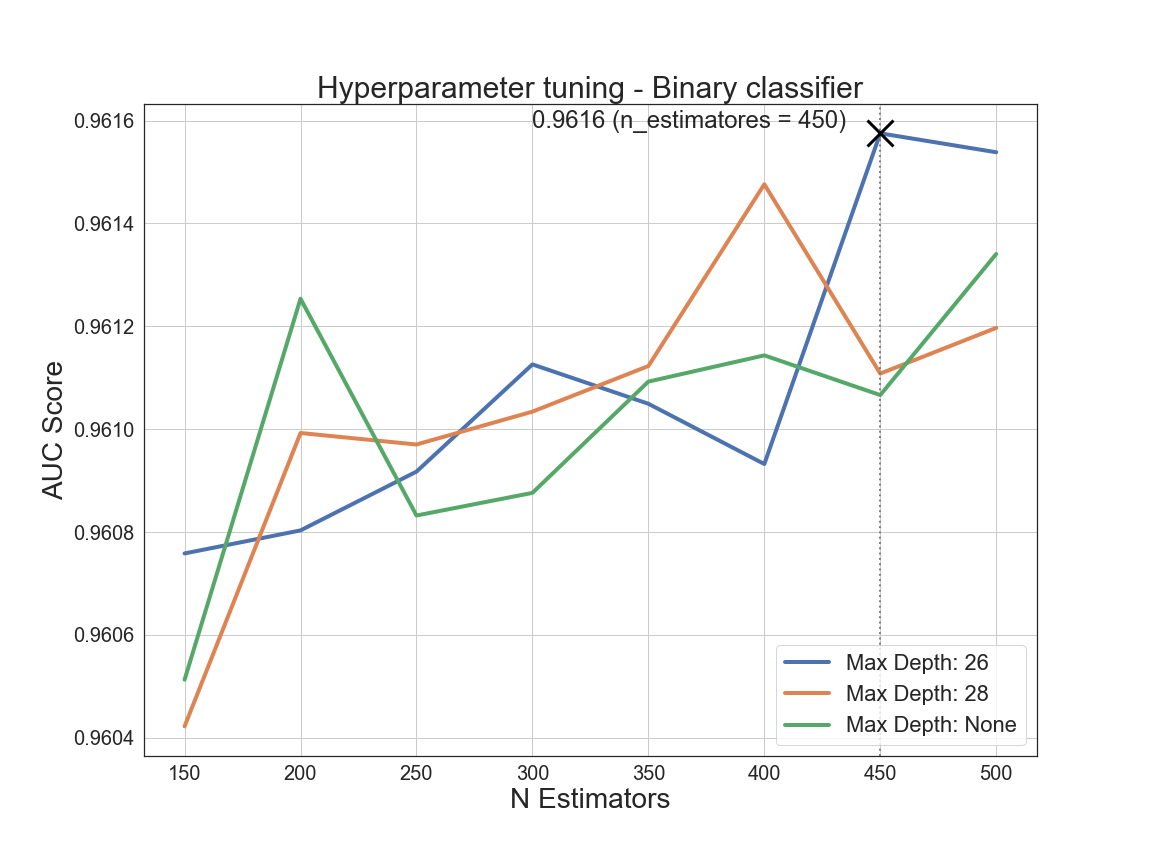
\includegraphics[width=\columnwidth]{chapter5/figure/bon_tuning.png}
	\caption{Grid search results}
	\label{fig:grid_search}
\end{figure}
\begin{figure}[htp!]
	\centering
	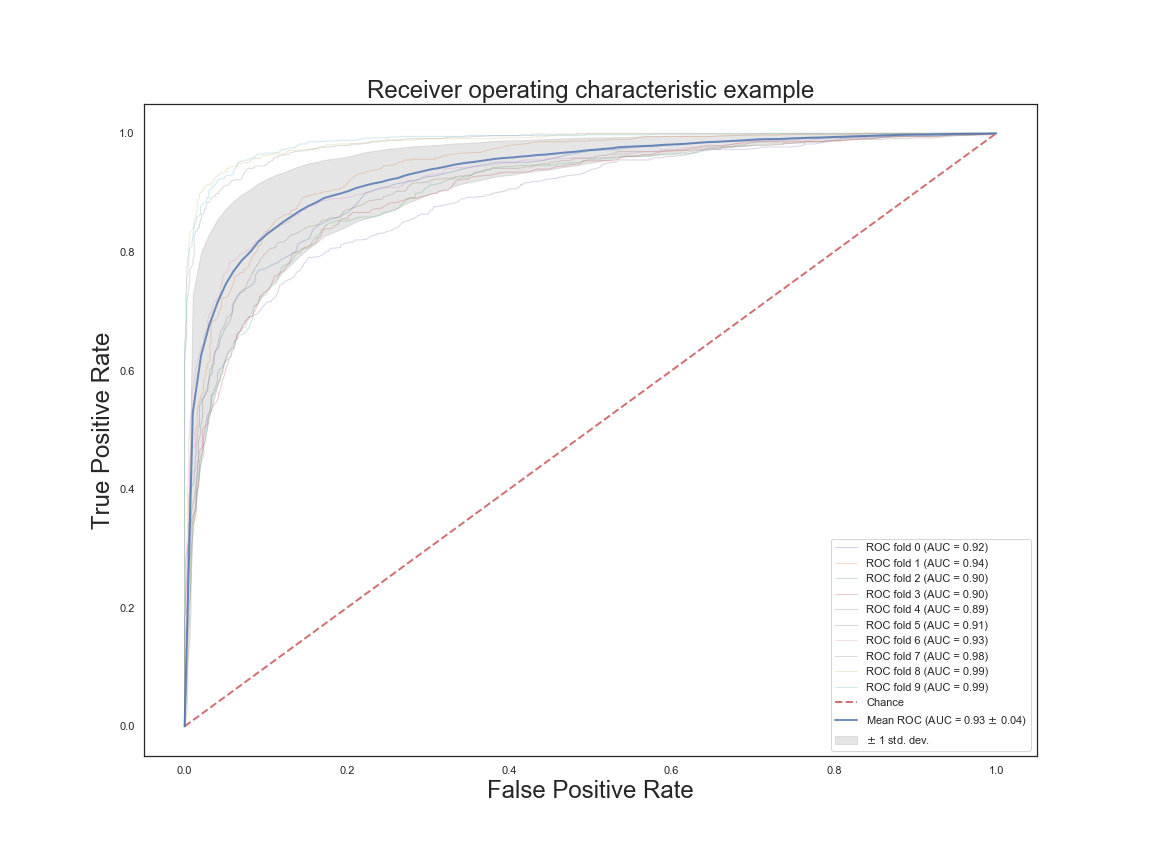
\includegraphics[width=\columnwidth]{chapter5/figure/auc.png}
	\caption{ROC curve}
	\label{fig:auc}
\end{figure}
As we can see in Figure \ref{fig:grid_search}, the AUC is increasing with the number of the estimators in the forest. We decided t stop at 450, which corresponds to the highest AUC score, since this phase was aimed to find a comparison term with Botometer, but it didn't represent the final model.
In their paper \cite{Varol}, the Botometer group claims to reach 0.95 in AUC score.

The AUC obtained with our arrangement is equal to 0.96, as shown in Figure \ref{fig:auc}, which is a positive accomplishment, considering that it will be used only as support for the identification of humans among bots, but we didn't crafted specific features as the ones involved in the Botometer project and we didn't have the same amount of data neither.

The model has then been fitted with the hole data, with this settings: \textit{ n\_estimators} = 450, \textit{max\_depth} = 26 and \textit{criterion} = 'entropy'.

\subsection{Validation}

We had an interesting amount of data that were not involved in this task, because of the comparison with the same Botometer's dataset. Since this unseen data had a further discrimination among bots, it was easy to sample some records randomly, replacing their multi-class targets with binary values.
We performed this job to validate the newborn model on unseen and fresher data.
We were interested in testing a model that were trained over ``old`` accounts, with consequent different attributes values and different behaviours on the platform, with younger accounts.

This validations would had given us a preview of the real performance of the model, once it would had been deployed on the internet. The account that a user would test with our application could be younger than the ones included in the Caverlee's list.

We sampled 6,000 accounts, divided in 3,000 genuine and 3,000 bot ids, randomly picked by our multi-class dataset.

The binary model were fitted with its data and it was ready to perform new predictions.

Looking at the most relevant features for the classifier, as shown in Figure \ref{fig:bon_importances}, we could find the \textbf{age} field at the top position.

\begin{figure}[htp!]
	\centering
	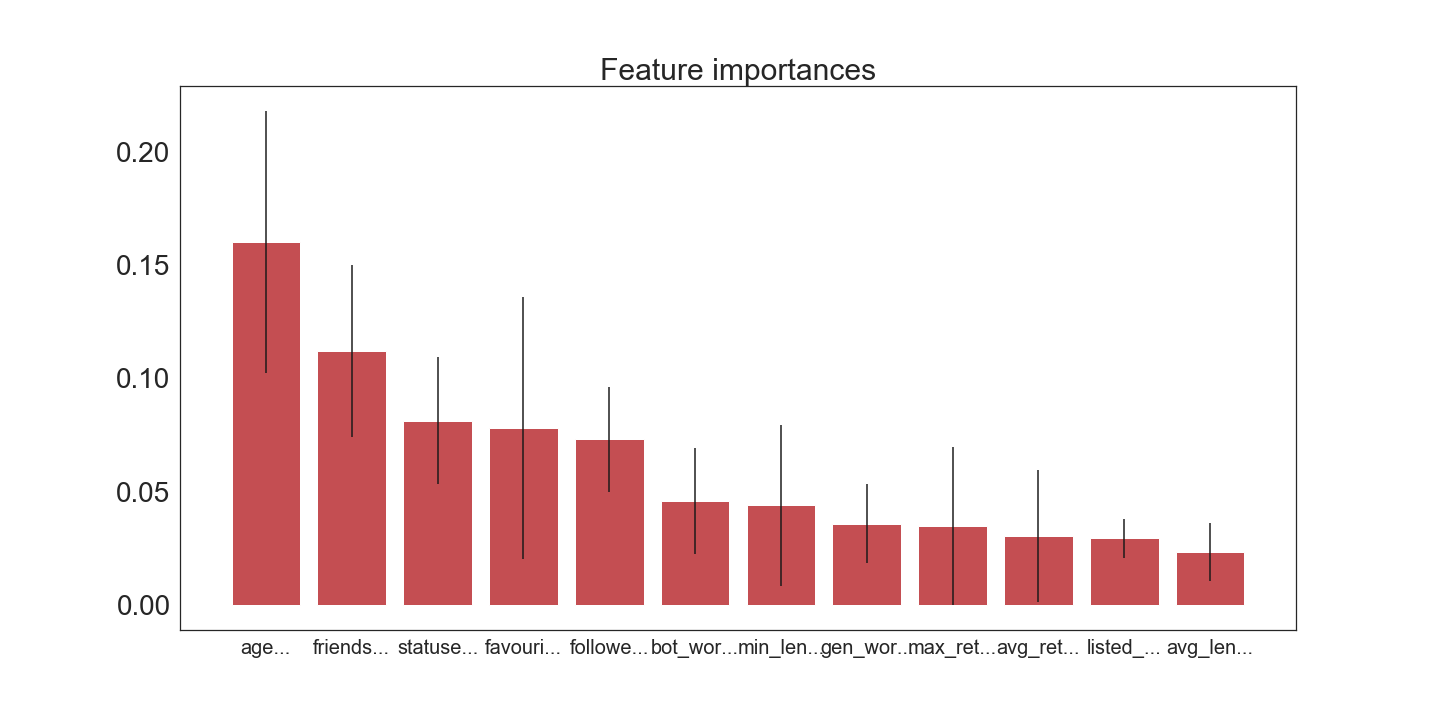
\includegraphics[width=\columnwidth]{chapter5/figure/bon_importances.png}
	\caption{Binary Random Forest features ranking}
	\label{fig:bon_importances}
\end{figure}

This was the first warning of a validation performance worsening.
A said before, the age of the accounts in the Caverlee's dataset were higher than the ones in our dataset. In particular, we examined the \textit{age} field of the training set, and the one coming from our validation samples, picked from the mutliclass dataset.
\begin{table}[!htb]
	\caption{Age field comparison among bot accounts}
	\begin{center}
		\begin{tabular}{@{}lr@{}}
			\multicolumn{2}{c}{\textbf{Training Bots}}\\
			\hline\hline
			\multicolumn{2}{c}{\textit{age}}\\
			\hline
			\multicolumn{1}{l}{mean}& \multicolumn{1}{r}{8}\\
			\multicolumn{1}{l}{std}& \multicolumn{1}{r}{0.66}\\
			\multicolumn{1}{l}{min}& \multicolumn{1}{r}{4}\\
			\multicolumn{1}{l}{max}& \multicolumn{1}{r}{12}\\
			\multicolumn{1}{l}{25\%}& \multicolumn{1}{r}{8}\\
			\multicolumn{1}{l}{50\%}& \multicolumn{1}{r}{9}\\
			\multicolumn{1}{l}{75\%}& \multicolumn{1}{r}{9}\\
			\hline\hline
		\end{tabular}
		\begin{tabular}{@{}lr@{}}
			\multicolumn{2}{c}{\textbf{Validation Bots}}\\
			\hline\hline
			\multicolumn{2}{c}{\textit{age}}\\
			\hline
			\multicolumn{1}{l}{mean}& \multicolumn{1}{r}{4.50}\\
			\multicolumn{1}{l}{std}& \multicolumn{1}{r}{2.69}\\
			\multicolumn{1}{l}{min}& \multicolumn{1}{r}{0}\\
			\multicolumn{1}{l}{max}& \multicolumn{1}{r}{11}\\
			\multicolumn{1}{l}{25\%}& \multicolumn{1}{r}{3}\\
			\multicolumn{1}{l}{50\%}& \multicolumn{1}{r}{4}\\
			\multicolumn{1}{l}{75\%}& \multicolumn{1}{r}{6}\\
			\hline\hline
		\end{tabular}
	\end{center}
	\label{table:bots}
\end{table}


\begin{table}[!htb]
	\caption{Age field comparison among genuine accounts}
	\begin{center}
		\begin{tabular}{@{}lr@{}}
			\multicolumn{2}{c}{\textbf{Training Genuine}}\\
			\hline\hline
			\multicolumn{2}{c}{\textit{age}}\\
			\hline
			\multicolumn{1}{l}{mean}& \multicolumn{1}{r}{9.22}\\
			\multicolumn{1}{l}{std}& \multicolumn{1}{r}{0.54}\\
			\multicolumn{1}{l}{min}& \multicolumn{1}{r}{4}\\
			\multicolumn{1}{l}{max}& \multicolumn{1}{r}{12}\\
			\multicolumn{1}{l}{25\%}& \multicolumn{1}{r}{9}\\
			\multicolumn{1}{l}{50\%}& \multicolumn{1}{r}{9}\\
			\multicolumn{1}{l}{75\%}& \multicolumn{1}{r}{9}\\
			\hline\hline
		\end{tabular}
		\begin{tabular}{@{}lr@{}}
			\multicolumn{2}{c}{\textbf{Validation Genuine}}\\
			\hline\hline
			\multicolumn{2}{c}{\textit{age}}\\
			\hline
			\multicolumn{1}{l}{mean}& \multicolumn{1}{r}{6.40}\\
			\multicolumn{1}{l}{std}& \multicolumn{1}{r}{1.94}\\
			\multicolumn{1}{l}{min}& \multicolumn{1}{r}{3}\\
			\multicolumn{1}{l}{max}& \multicolumn{1}{r}{11}\\
			\multicolumn{1}{l}{25\%}& \multicolumn{1}{r}{5}\\
			\multicolumn{1}{l}{50\%}& \multicolumn{1}{r}{6}\\
			\multicolumn{1}{l}{75\%}& \multicolumn{1}{r}{8}\\
			\hline\hline
		\end{tabular}
	\end{center}
	\label{table:genuine}
\end{table}

Like Tables \ref{table:bots} and \ref{table:genuine} show, there is a clear differences in the age attribute, between training and validation set.

We went forward to check if this diversity would had led us to a bad validation performance, or if the model would had handled the predictions in other ways.

The 10-fold crossvalidation on the validation set produced the following confusion matrix, with the correlated AUC score:\\

{
	\centering
	\begin{tabular}{@{}cc|cc@{}}
		\multicolumn{1}{c}{} &\multicolumn{1}{c}{} &\multicolumn{2}{c}{Predicted class} \\ 
		\multicolumn{1}{c}{} & 
		\multicolumn{1}{c|}{} & 
		\multicolumn{1}{c}{BOT} & 
		\multicolumn{1}{c}{GEN}  \\
		\cline{2-4}
		\multirow[c]{2}{*}{Actual class}
		& BOT  & 558 & 2442\\
		& GEN  & 158 & 2842\\
		\cline{2-4}
		\multicolumn{2}{r|}{AUC} & 
		\multicolumn{2}{l}{0.566}\\
		\multicolumn{4}{c}{}\\
	\end{tabular}\\
}
The worsening were real, and it highlighted the short-sighted training phase we performed, trying to top the Botometer performance.

We tried to mitigate this performance loss, by excluding the main suspect from the features set.
Here is the validation performance, without considering the accounts' ages.

{
\centering
\begin{tabular}{@{}cc|cc@{}}
	\multicolumn{1}{c}{} &\multicolumn{1}{c}{} &\multicolumn{2}{c}{Predicted class} \\ 
	\multicolumn{1}{c}{} & 
	\multicolumn{1}{c|}{} & 
	\multicolumn{1}{c}{BOT} & 
	\multicolumn{1}{c}{GEN}  \\
	\cline{2-4}
	\multirow[c]{2}{*}{Actual class}
	& BOT  & 2920 & 20\\
	& GEN  & 1589 & 1411\\
	\cline{2-4}
	\multicolumn{2}{r|}{AUC} & 
	\multicolumn{2}{l}{0.721}\\
	\multicolumn{4}{c}{}\\
\end{tabular}\\
}

The improvement was encouraging, but still not enough to rely on this basic solution.
Considering the bot target as the positive class, we still had too many False Positive in our confusion Matrix. The binary classifier used to tend to identify an user as a bot, with too much confidence. We had to reduce that number, in order to provide a reliable filter in the final prediction pipeline system.

\subsection{Data extension}
The idea we had was to use some data from our multi-class dataset to enrich the binary training set, in order to make the algorithm handle younger and different types of samples from the Twitter population.

In order to perform the extension, we sampled 3,000 genuine accounts and 8,000 bots (2,000 content polluters for each class), all coming from our dataset, and added them to the Caverlee's dataset.
The new training set was composed by 42,212 samples.

We performed a 10-fold-crossvalidation to see the effect of this data refill, sticking to the same hyperparameters found by the last Grid Search. The AUC score measured with these data was 0.963. We could see a slight improvement of the performances, with this data extension. However, we wanted to take a look inside the inner ranking performed by the algorithm, to check if the age field represented an important splitting point.
Figure \ref{fig:bon_importances_ext} shows that the age attribute was still the most considered when the trees had to perform the first splits.

We couldn't blindly follow the AUC score through Grid Searches, without making considerations about what will happen when we will allow people to classify data coming from outside our collected samples.
The age feature would have driven the Random Forest to misclassification over accounts with low \textit{age} values.
Even if the exclusion of that attribute would had made the overall AUC score worse, we had to strip it from the features vector, in order to better generalize on real test cases.

\begin{figure}[htp!]
	\centering
	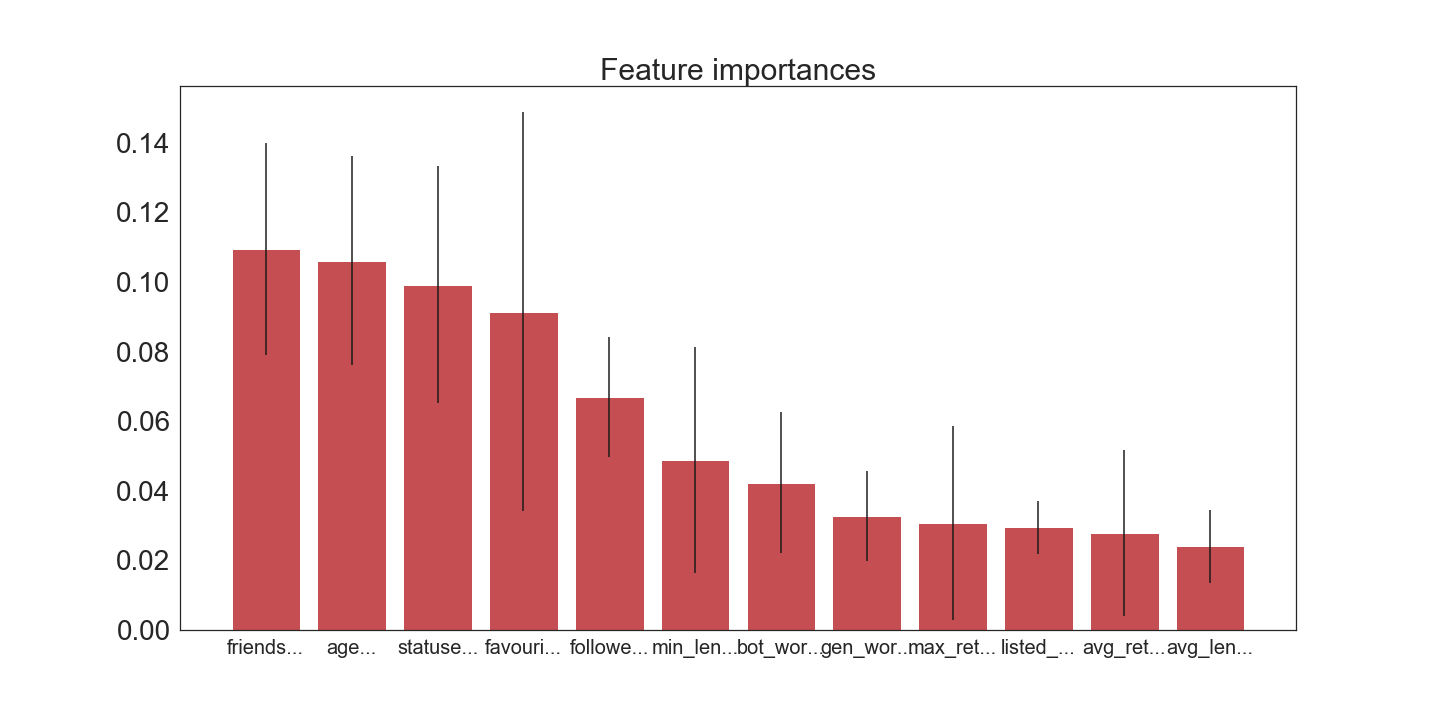
\includegraphics[width=\columnwidth]{chapter5/figure/bon_importances_extensions.png}
	\caption{Features ranking with augmented data - Top 12 }
	\label{fig:bon_importances_ext}
\end{figure}

While cross-validating the model, we tested the complete features vector (with and without the extension from our dataset) and the one stripped by the age values. The crossvalidation was performed with the same hyperparameters settings of the model fitted with the Caverlee's dataset only.

{
	\centering
	\begin{tabular}{@{}cccc@{}}
		\multicolumn{1}{c}{} & 
		\multicolumn{3}{c}{Fitted data} \\ 
		\cline{2-4}
		\multicolumn{1}{c|}{} & 
		\multicolumn{1}{c|}{original - with \textit{age} } & 
		\multicolumn{1}{c|}{extended - with \textit{age} } & 
		\multicolumn{1}{c|}{extended - without \textit{age}} \\
		\cline{1-4}
		\multicolumn{1}{|c|}{AUC} & 
		\multicolumn{1}{c|}{\textbf{0.961}} & 
		\multicolumn{1}{c|}{\textbf{0.963}} & 
		\multicolumn{1}{c|}{\textbf{0.948}} \\
		\cline{1-4}\\
	\end{tabular}\\
}

The age filed removing made thing worse, but we decided to perform it anyway, because of the good score reached without it, and the flexibility we were giving to the Random Forest. The slight worsening could be also imputed to the biased extrinsic features of that data: those samples came from the multi-class dataset and they originally had the extrinsic features based on the four bot categories' dictionaries.
In order to refill the binary dataset with these new samples, we had to recompute the extrinsic features, applying the analogous method used for the binary purpose.
We didn't recompute the entire dictionaries, we just assigned the scores to the new samples we were introducing, basing the calculations on the already listed words. Those had been exposed in chapter \ref{capitolo4}. This approach aimed to force the algorithm to identify bots and humans, basing its comparisons on the online computations of those features, like in a real-case generalization.

This last configuration was used to performed a further tuning of the parameters.
A new Grid Search brought us the configuration for the hyperparameters shown in Figure \ref{fig:bon_tuning_refil}, leading to the new AUC score, exposed in Figure \ref{fig:bon_refil_auc}.
\begin{figure}[htp!]
	\centering
	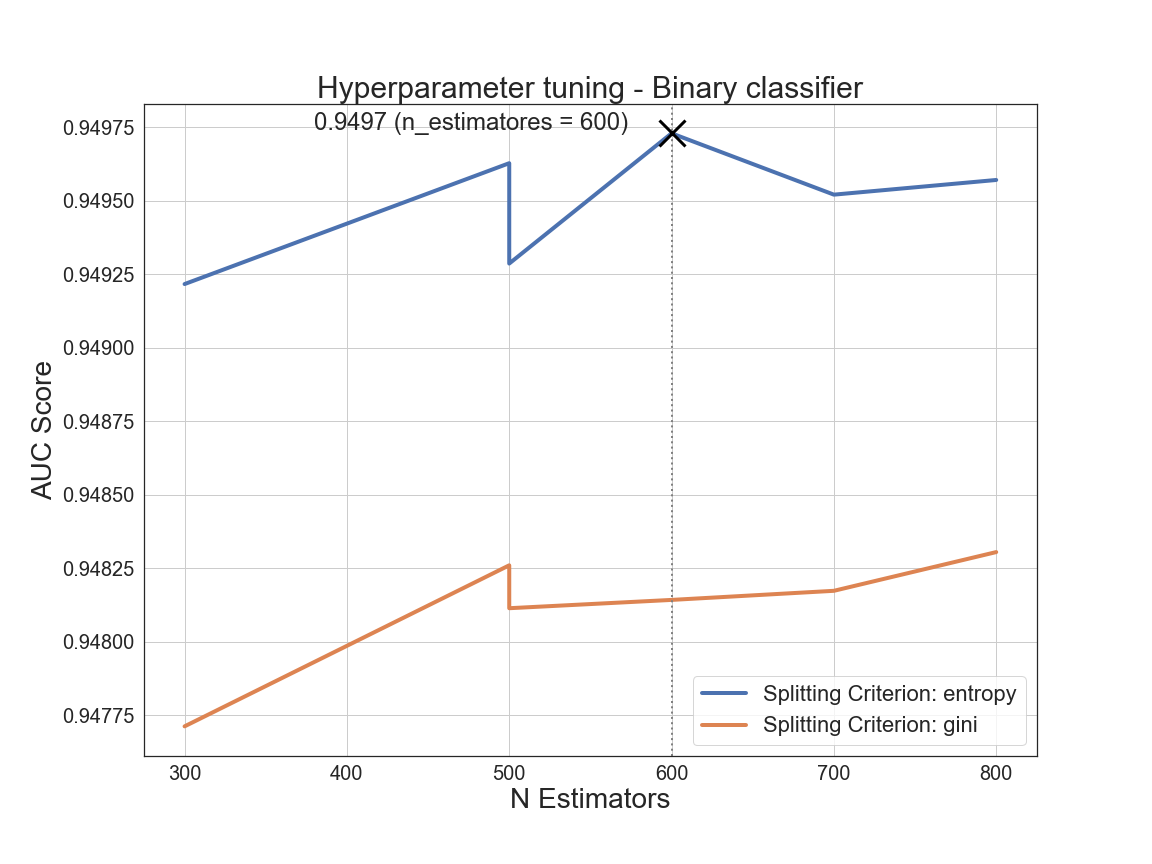
\includegraphics[width=\columnwidth]{chapter5/figure/bon_tuning_refill.png}
	\caption{Grid Search with extended data}
	\label{fig:bon_tuning_refil}
\end{figure}
\begin{figure}[htp!]
	\centering
	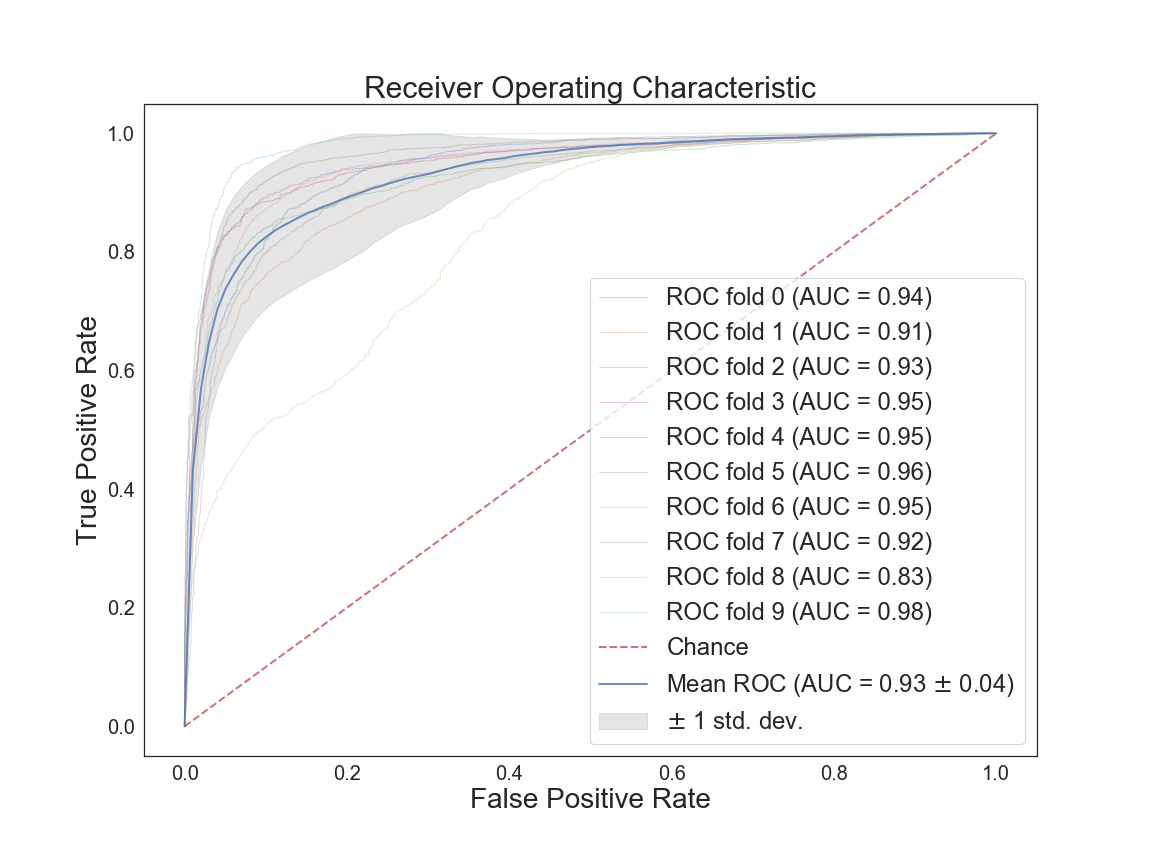
\includegraphics[width=\columnwidth]{chapter5/figure/refill_auc.png}
	\caption{AUC score with extended data}
	\label{fig:bon_refil_auc}
\end{figure}
The binary classifier has then been fitted with 42,212 samples with 34 features, 600 estimators, entropy splitting criterion and 26 levels of maximum depth.

\section{Multi-class ensemble classifier}
It somehow represents the core of our thesis, it models the starting idea: go deep inside bot identification and search and classify similar behaviours among them.

In this section we will expose the model involved in the multi-class ensemble. In this process, we used a Random Forest algorithm, working on all the crafted features; a KNN model, operating on the user attributes only; a final text-based Naive Bayes classifier, which reads the tweets' texts and classifies them.

At first, this ensemble of these three models should have been blended with the prediction of the binary classifier. That means that the genuine class was part of the labels we were trying to classify, even in the multi-class models. Then, we found an issue in this approach: the binary classifier itself wasn't enough, even including it into the ensemble, to give the right importance to the genuine accounts. This problem emerged because of the others classifiers, as they were trying to classify the genuine class too. They lacked in data with that target, so, basically, they used to treat that category as one other of the bot types.

Even if the results on our validation sets were still good (we accomplished a F1 measure of 0.973), for the final ensemble method, we knew that this method would had yielded to a poor bot vs genuine detection tool. We couldn't accept that situation, because, in order to go deeper than other works, in bot behaviour classifications, we had to provide a solid previous discrimination between humans and automated accounts.

The ensemble method with all the classifiers blended together were replaced with a pipeline, and the multi-class models were trained on bot categories only.
These last classifiers had been put together inside a  ensemble, which returns the final mutliclass probability prediction, based on the opinions of those models, as shown in Figure \ref{fig:stacking_schema}

The different nature of the classifiers, and the feature subsets as well, is one of the strengths of the stacking approach: it combines different opinions about the samples, driven by different classifiers, considering different parameters and attributes; basing on those unlike classifications, it builds its own.

It differs from other ensemble methods as bagging and boosting, because of this miscellaneous schema, and it can be a robust method to exploit the different characteristics of the classifiers stacked together.

\begin{figure}[htp!]
	\centering
	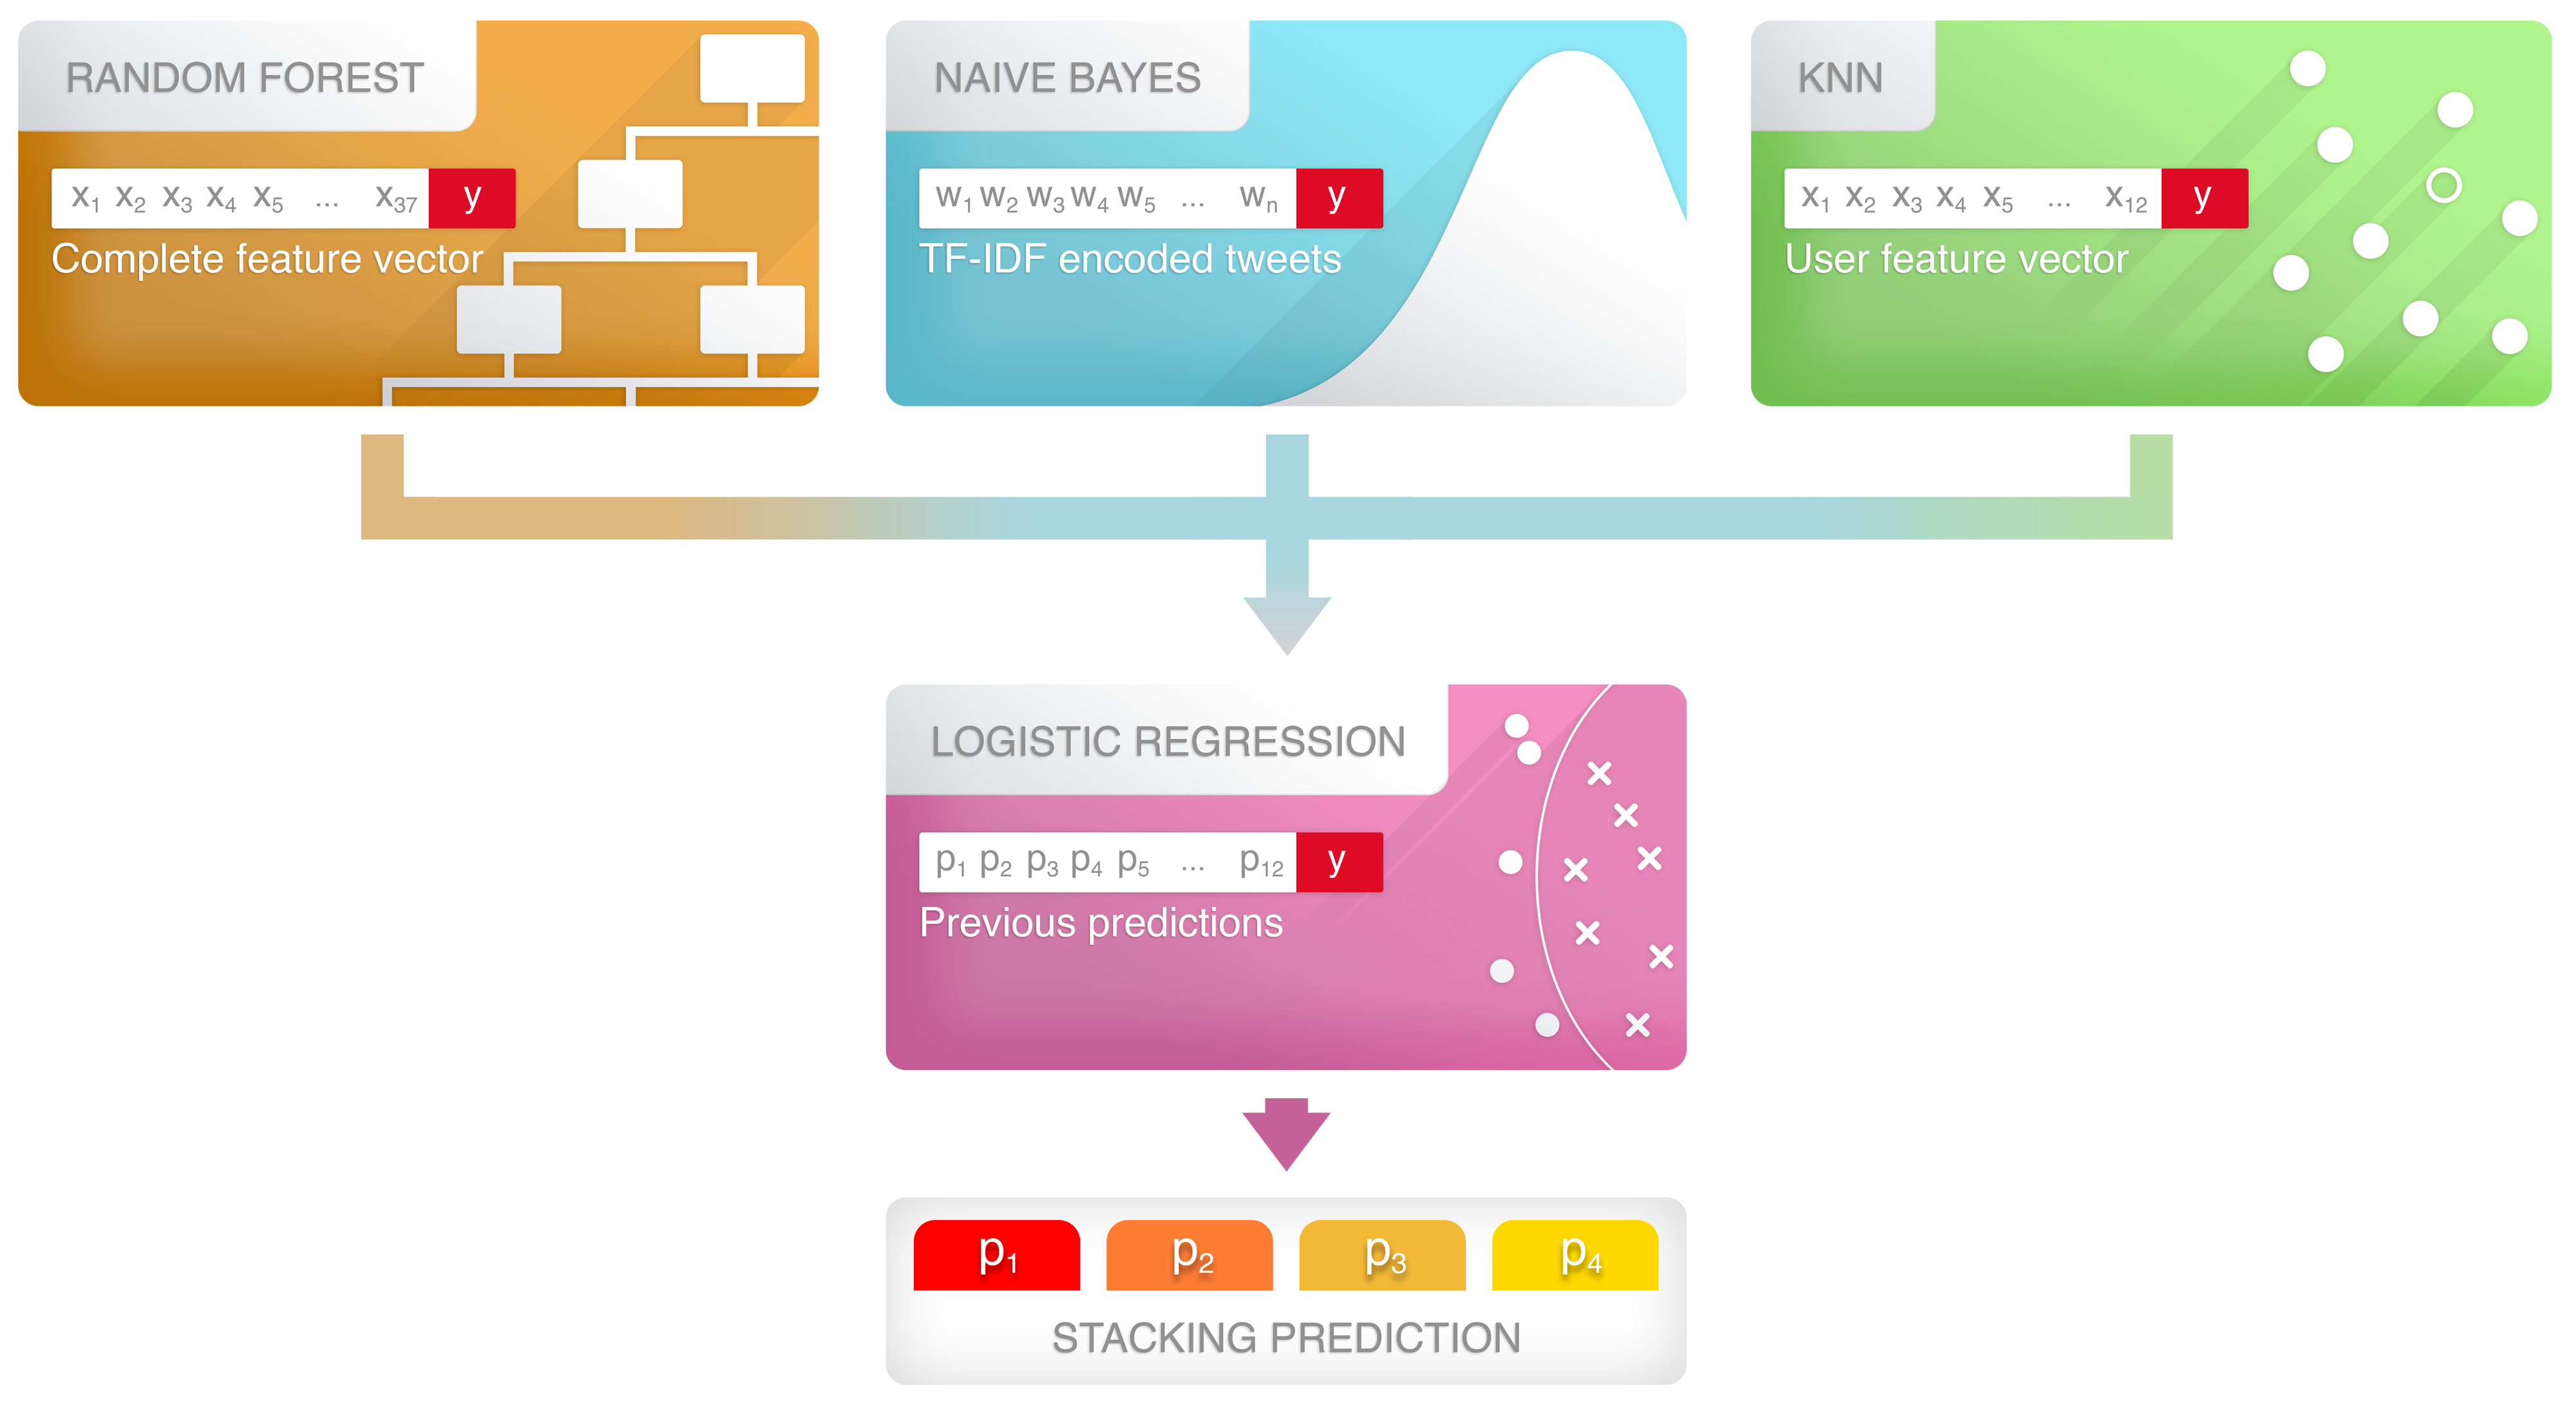
\includegraphics[width=\columnwidth]{chapter5/figure/stacking.png}
	\caption{Multi-class ensemble schema}
	\label{fig:stacking_schema}
\end{figure}
In the following subsections there are the detailed explanations of the three classifier announced before.

\subsection{All-features-based Random Forest classifier}
\subsubsection{Dataset}
During this phase, we used the previously described dataset \ref{sec:dataset} with its four different labels.
The algorithm was fed with 21,445 samples and 37 features. the amount of records were light enough to consider K-fold crossvalidation, without slow the validation down too much.
\subsubsection{Model}
We found ourselves in the situation in which we had some brand new features and we didn't know how useful they were. Obviously, we could appeal to heat-maps or other tools, to highlight the correlations among variables and targets.
However, the model we wanted to develop was the Random Forest, which proved to perform well with F1 score. Since this kind of model exploits its criteria to employ the features, we needed to prove them with a direct approach.

\subsubsection{Features selection}
A useful advantage of the Random Forest algorithm is the ability to provide a feature ranking, according to its splitting criterion.
We retrieved this standing, in order to see if we would have found some of the ones coming out from feature engineering at the top positions.
The algorithm ranking ranked the features this way: 1. \textit{favourites\_count} (0.179), 2. \textit{nsfw\_profile} (0.068), 3. \textit{freq} (0.061), 4. \textit{tweet\_intradistance} (0.060), 5. \textit{news\_spreaders\_words\_score} (0.058), 6. \textit{statuses\_count} (0.053), 7. \textit{avg\_len} (0.051), 8. \textit{followers\_count} (0.051), 9. \textit{NSFW\_words\_score} (0.043), 10. \textit{ret\_perc} (0.041), 11. \textit{min\_len} (0.038), 12. \textit{spam\_bots\_words\_score} (0.035), ...  37. \textit{min\_fav} (0.0001).

\begin{figure}[htp!]
	\centering
	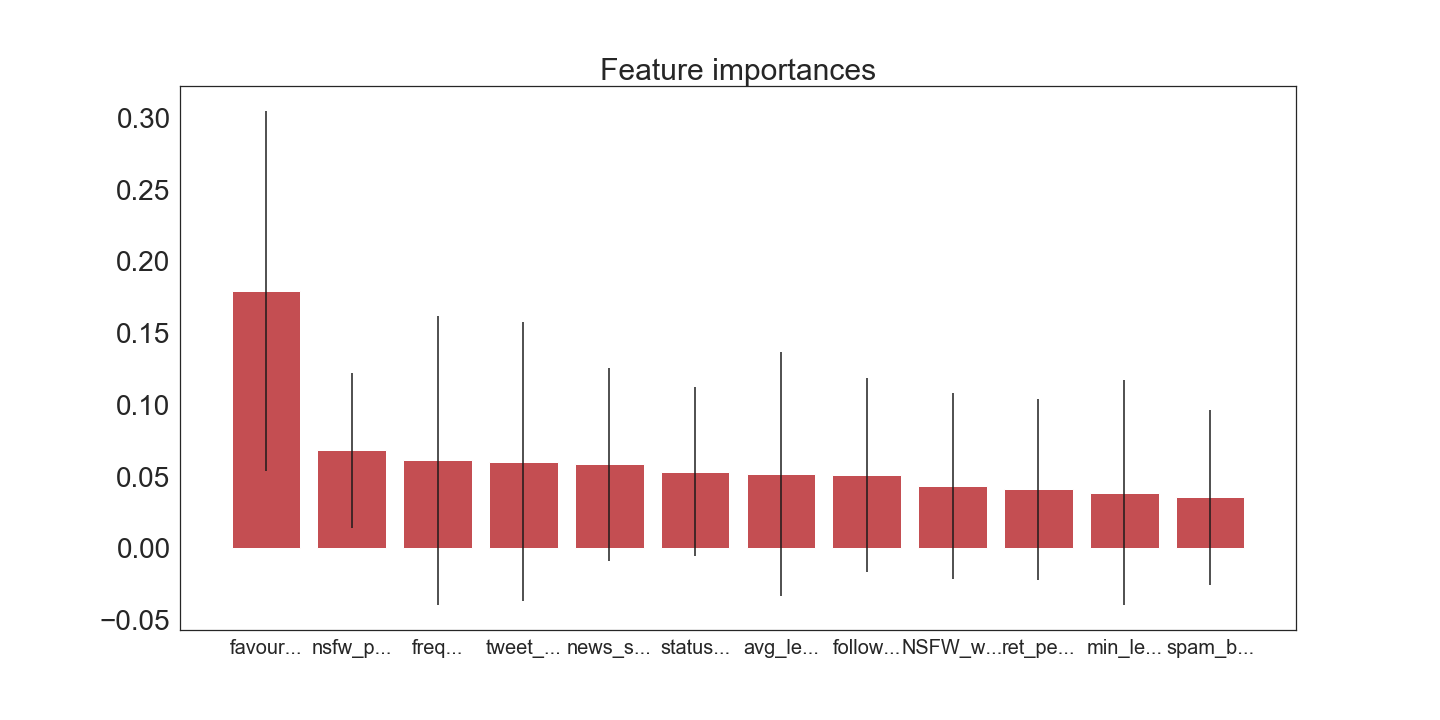
\includegraphics[width=\columnwidth]{chapter5/figure/top_12_features_importances.png}
	\caption{Random Forest top-12 feature ranking}
	\label{fig:feature_rank}
\end{figure}

As Figure \ref{fig:feature_rank} shows, we could find some of our crafted features inside this list: lots of tweets descriptive features (\textit{avg\_len, freq, ret\_perc}, etc...), as well as the \textit{tweet\_intradistance} attribute and three of the four extrinsic features, like \textit{news\_spreaders\_words\_score}, \textit{NSFW\_words\_score} and the \textit{spam\_bots\_words\_score}.
This picture confirmed us that the idea behind those features was useful.

Since those attributes were thought to belong to different clusters, we decided to try several combinations of those feature clusters, validating the model on them with a crossvalidation. The purpose of this stage was to see if some groups of features were enough to describe the real problem, or if some group would shown up as irrelevant.
To face this evaluation, we performed a light-weighted Grid Search, which is a method that takes desired ranges of hyperparameters and tries all the possible permutations of them, looking for the best combination, in terms of a certain metric.

We are talking about a light-weight version of this tool, because we just went through different numbers of tree estimators in the forest. The different feature groups are not considered as hyperparameters and are not handled by the Scikit-learn implementation of the Grid Search.
We had to manage the different training by our own, looking how the test score would have changed along with the increasing number of estimators and the different set of features.

Grid Search uses crossvalidation to find the better estimators for the models, and this approach was right for our situation.
Due to the multi-class nature and some imbalances with the labels, we decided to follow the F1 score metric to asses the value of our model.

The features were organized in clusters, as described in Chapter \ref{capitolo4}.
We had the user features, the descriptive features, the intrinsic features, the extrinsic and the image features. Then we tried the model with the entire set of 38 attributes.
As shown in Figure \ref{fig:feature_clusters}, the best configuration seems to involve the whole set of features, as it reaches these scores, with 100 estimators: \textit{Precision} = 0.978, \textit{Recall} = 0.976, \textbf{\textit{F1}}= 0.977.

\begin{figure}[htp!]
	\centering
	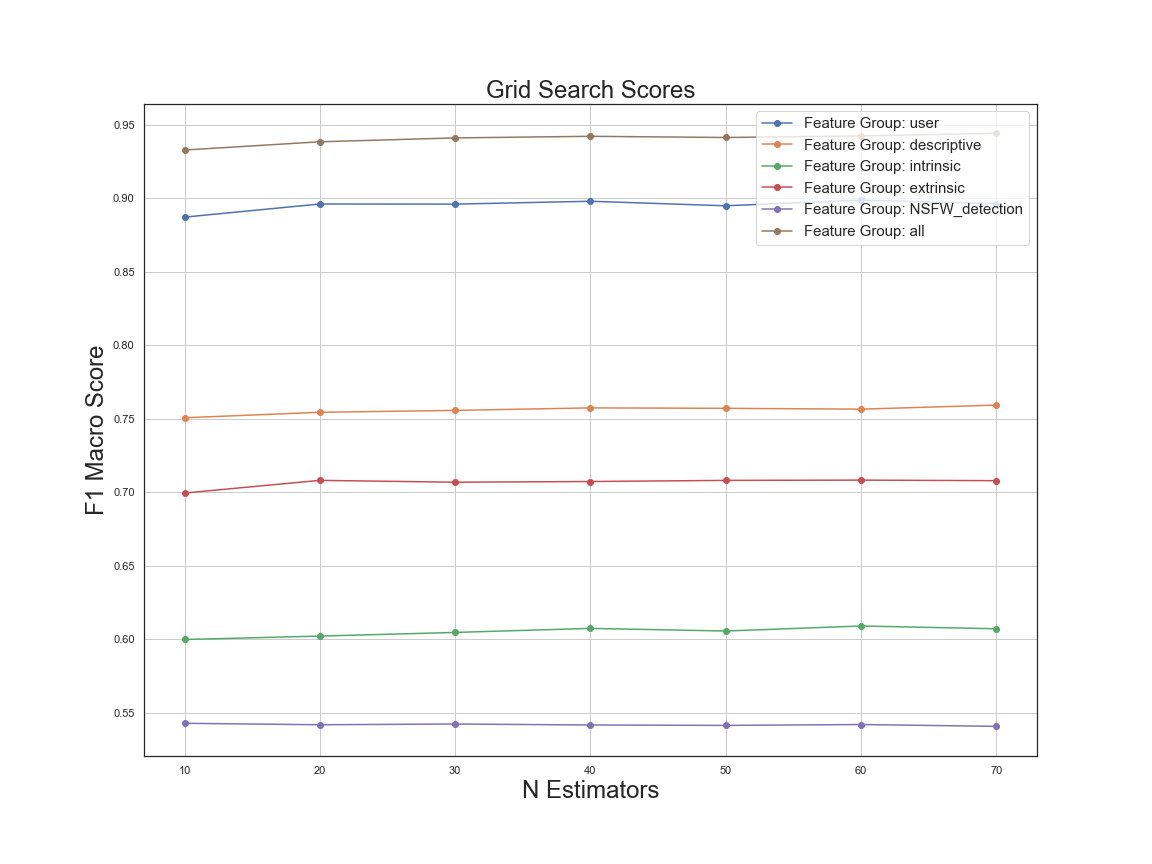
\includegraphics[width=\columnwidth]{chapter5/figure/feature_cluster_f1.png}
	\caption{Performance over different feature clusters}
	\label{fig:feature_clusters}
\end{figure}

The model has been tested with the default value for the maximum depth in the trees, which is set to 'None'. It means that the trees are expanded until every leaf is pure, or all leaves contain one sample.

In order to try all the alternatives, we setted a test involving the performance of the model, when it was working on an increasing number of features.
We had the ranking provided by the forest itself, so we started by testing only the most important attribute, adding one feature at time, until the least important was included.
We were looking for some changing in the scores, that would have pointed to a lighter model, with the exclusion of some features.
Figures \ref{fig:feat_prec}, \ref{fig:feat_rec}, \ref{fig:feat_f1} show the trends of the Precision, the Recall and the F1, respectively, along with the number of features tested.
 \begin{figure}[htp!]
 	\centering
 	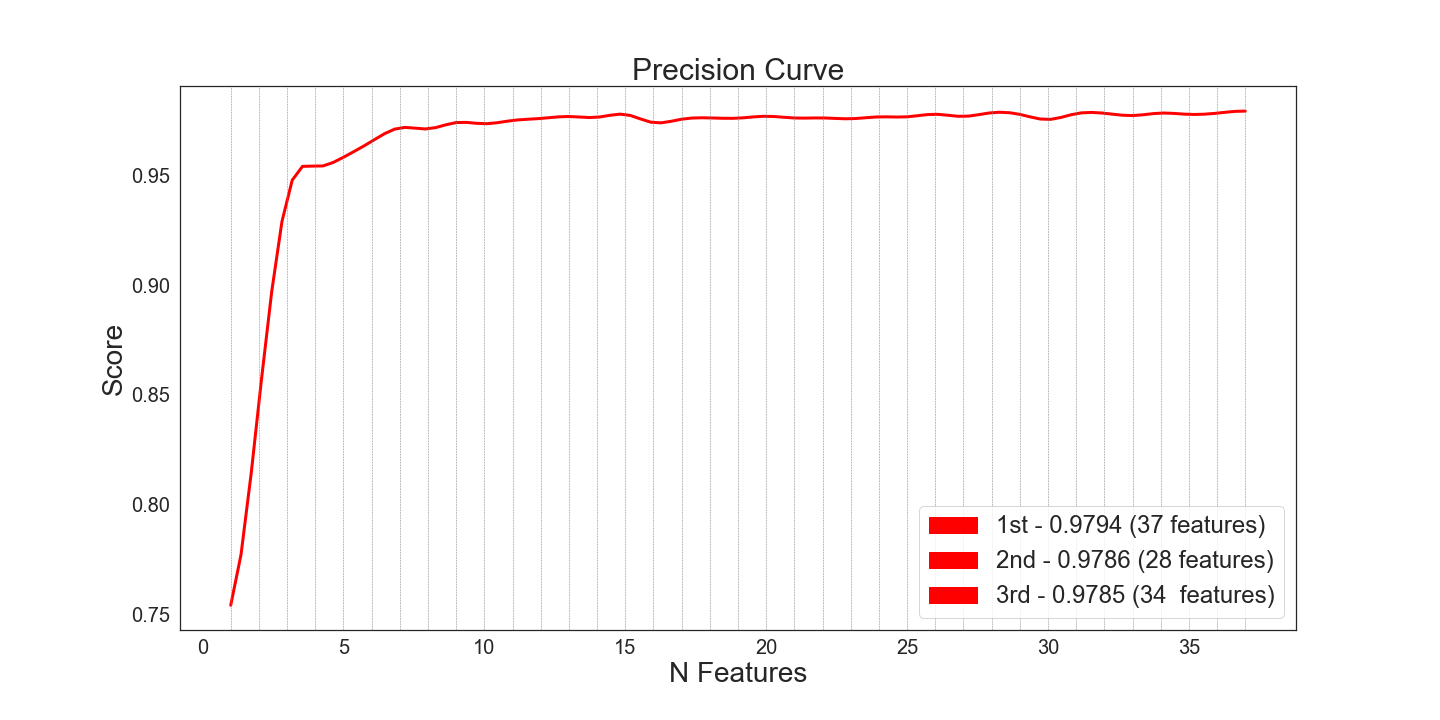
\includegraphics[width=\columnwidth]{chapter5/figure/precision_along_features.png}
 	\caption{Precision trend along with number of features tested}
 	\label{fig:feat_prec}
 \end{figure}
\begin{figure}[htp!]
	\centering
	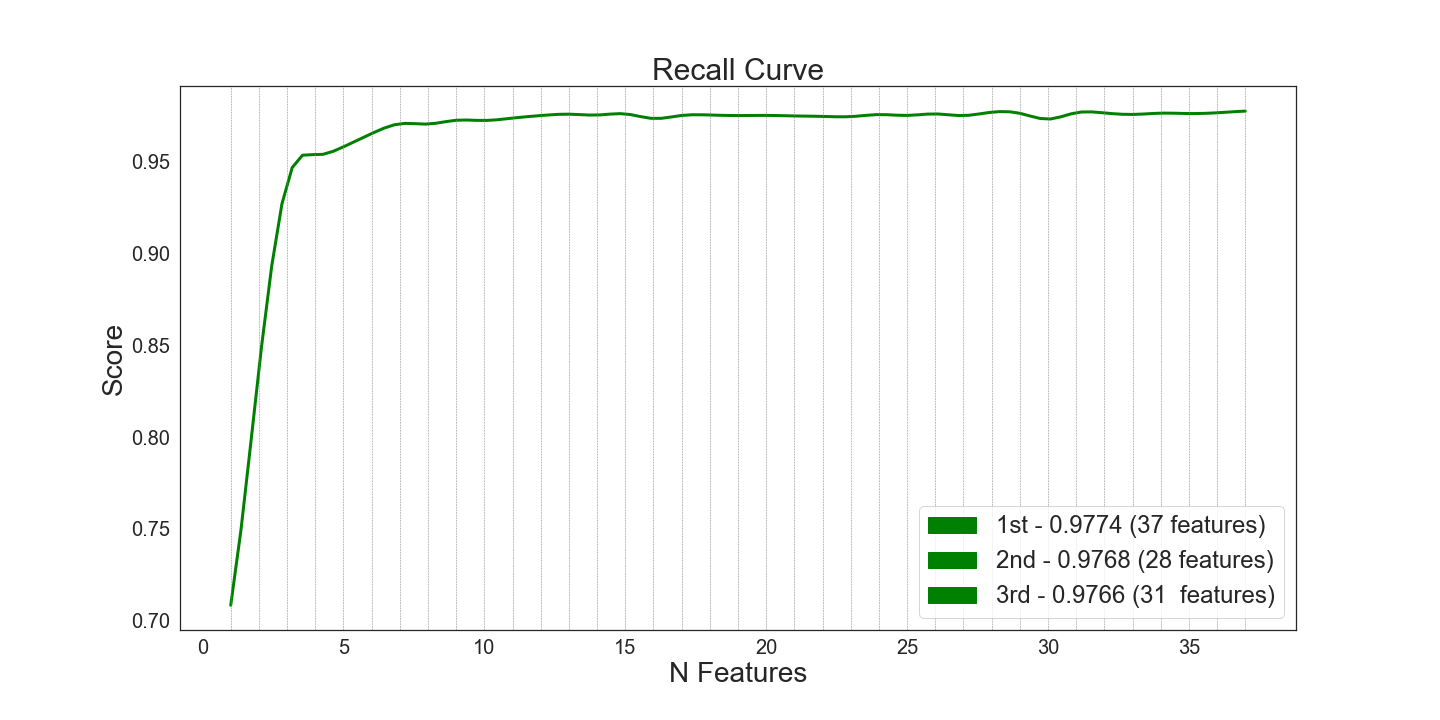
\includegraphics[width=\columnwidth]{chapter5/figure/recall_along_features.png}
	\caption{Recall trend along with number of features tested}
	\label{fig:feat_rec}
\end{figure}
\begin{figure}[htp!]
	\centering
	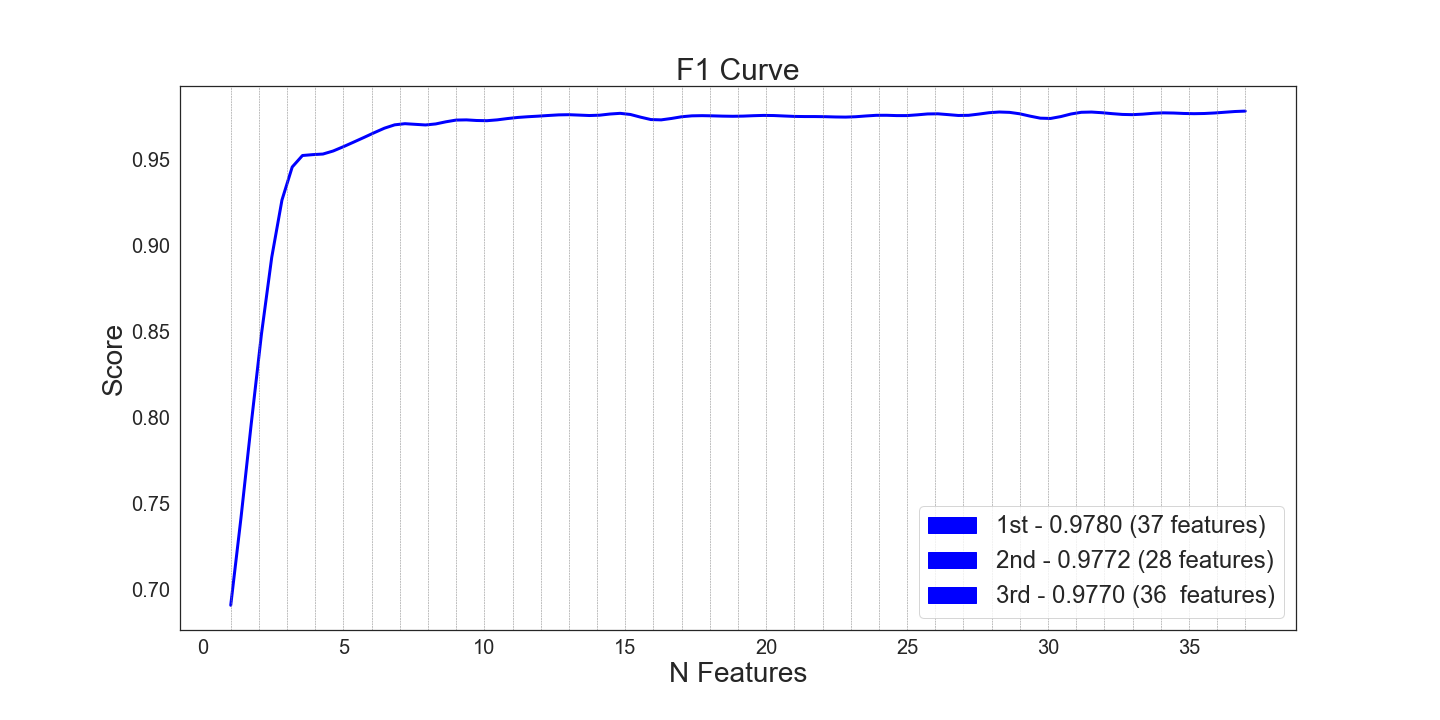
\includegraphics[width=\columnwidth]{chapter5/figure/f1_along_features.png}
	\caption{F1 trend along with number of features tested}
	\label{fig:feat_f1}
\end{figure}

As all the Figures show, the best solution possible, looking at both the three metrics, is the one involving all the 37 components of the feature vector.
There was the possibility to choose the second result, which wanted only the first 28 features, in terms of importance for the Random Forest. However, we weren't struggling with heavy models or long prediction times and the Random Forest algorithm handles the overfitting problem properly, even with complex models.
Thus, we moved on with the entire feature vector as support for the classification goal.

We then continued with a proper Grid Search over the whole number of features.
\subsubsection{Hyperparameters Tuning}
The algorithms rely on parameters in order to fit a problem.
Once the number of featured was picked, as well as the model, we needed to consider the possible hyperparameter ranges. 
The Grid Search method from Scikit-learn helped us, once again, during this exploration.
Since we were testing a Random Forest, we wanted to play with the number of estimators (tree) to include in the pool, as well as the maximum depth of each tree and the splitting criterion.

\begin{figure}[htp!]
	\centering
	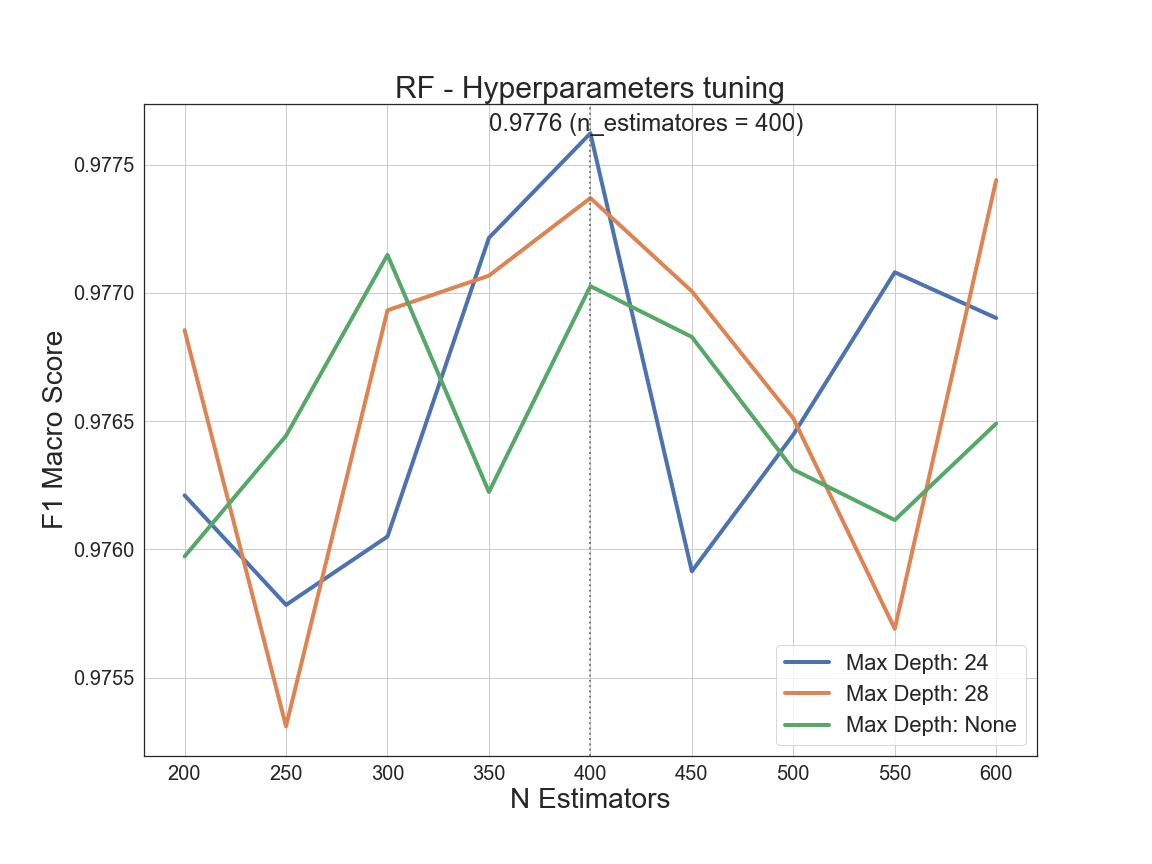
\includegraphics[width=\columnwidth]{chapter5/figure/multiclass_rf_tuning_gini.png}
	\caption{F1 scores with ``Gini`` criterion - close-up view}
	\label{fig:rf_tuning_gini}
\end{figure}
\begin{figure}[htp!]
	\centering
	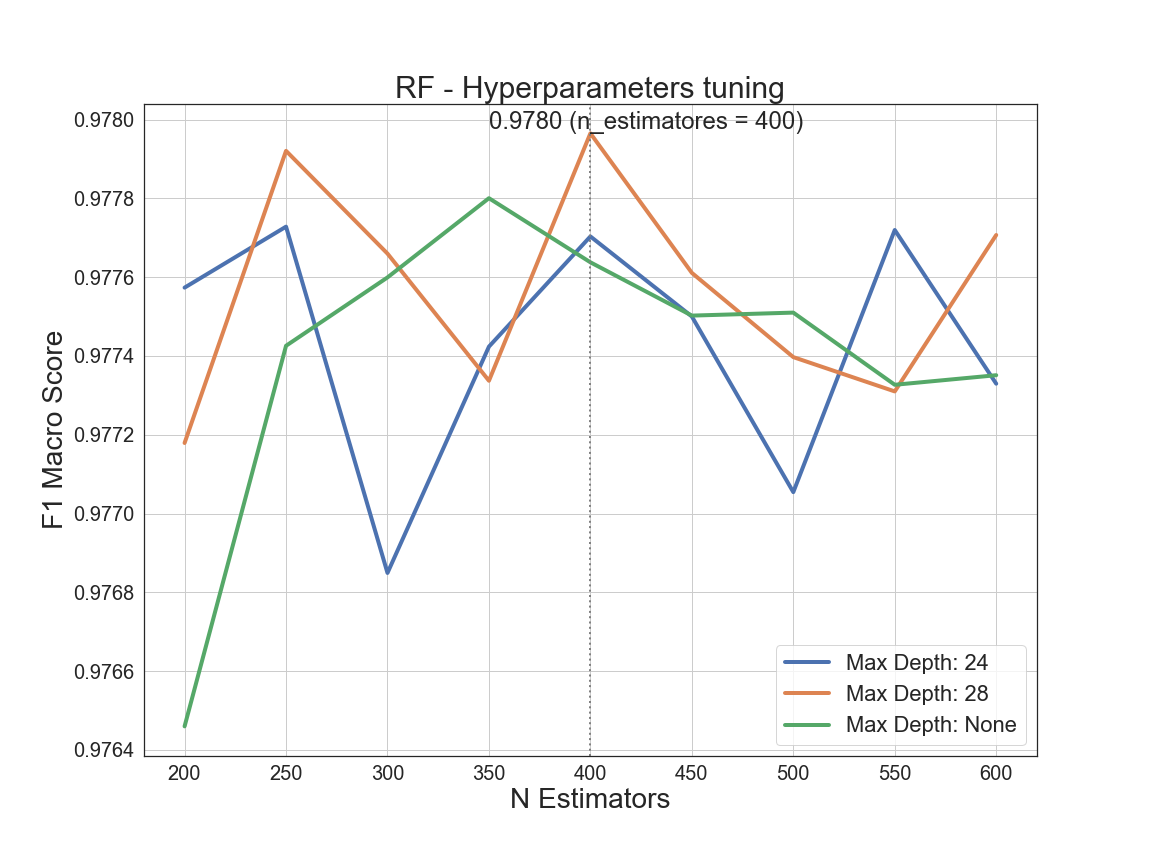
\includegraphics[width=\columnwidth]{chapter5/figure/multiclass_rf_tuning.png}
	\caption{F1 scores with ``Entropy`` criterion - close-up view}
	\label{fig:rf_tuning_entropy}
\end{figure}

The Figures \ref{fig:rf_tuning_gini}, \ref{fig:rf_tuning_entropy} show how the average F1 score, measured on 10-fold crossvalidation, changes with the increasing of the number of estimators in the forest.
The different coloured lines represent the \textit{max\_depth} hyperparameter.
The first Figure (\ref{fig:rf_tuning_gini}) shows the Grid Search results, with the \textit{gini} splitting criterion.
The second one (\ref{fig:rf_tuning_entropy}) represent the situation having \textit{entropy} as a splitting choice.
We combined nine numbers of estimators (200, 250, 300, 350, 400, 450, 500, 550, 600), together with three different maximum depths for the trees (26, 28, None) and the two above-mentioned splitting criteria.

We could observe a peak, for both criteria, in correspondence with 400 estimators.
Although the Gini-based forest's score didn't seem a bad point, we went with the Information Gain splitting criterion, which si also the same we used to rank the features of our data.

The final configuration involves 400 trees, the Information Gain criterion and the maximum reachable depth (for each of the 400 estimators) equal to 28 levels, yielding the following scores in 10-fold-crossvalidation:
\begin{itemize}
	\item[\PencilRight] \textit{Precision}: \textbf{0.979}
	\item[\PencilRight] \textit{Recall}: \textbf{0.977}
	\item[\PencilRight] \textit{F1 score}: \textbf{0.978}
\end{itemize}

Figure (\ref{fig:tree}) shows an example of one of the estimators of the final model, plotted with Matplotlib library for Python. It has been represented with the first two levels of depth, for visualizations reasons.

\begin{figure}[htp!]
	\centering
	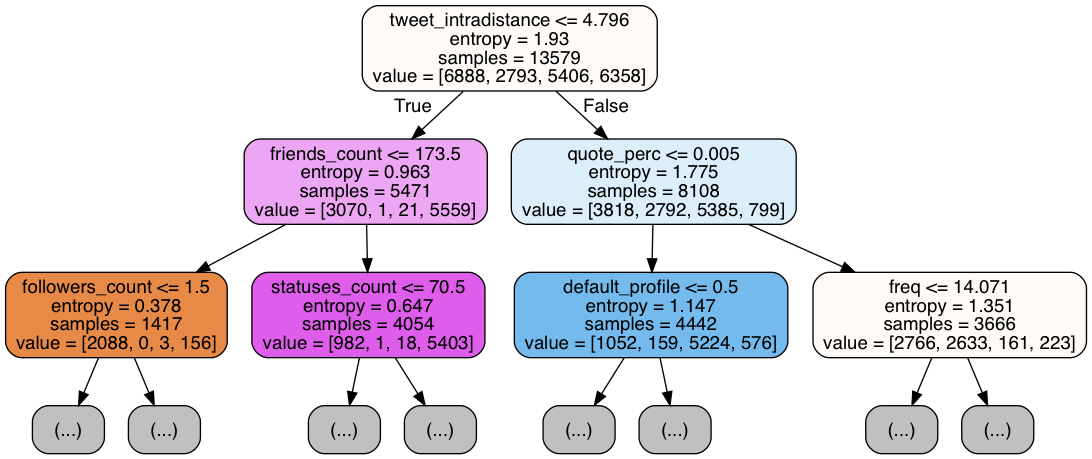
\includegraphics[width=\columnwidth]{chapter5/figure/tree.png}
	\caption{Tree estimator of the Random Forest model}
	\label{fig:tree}
\end{figure}

As the picture shows, this tree used the \textit{tweet\_intradistance} feature as root, in order to perform its first split on that attribute.

The first algorithm of the multi-class ensemble was completed and ready to be combined with the following models.

\subsection{User-based KNN classifier}
The Random Forest model represents somehow the core of the ensemble, as it was trained on the entire feature vector, with all the data we had for the purpose. A massive attention for parameters and features were given for that classifier. 
However, we wanted to put it into an ensemble, not to improve its already strong stability over outliers, but to support it with different perspectives.

We noticed, as shown in the previous Figure \ref{fig:feature_clusters}, that the user features were a good group to build a classifier on. Thus, we started thinking how to implement such support, and we basically looked at our baselines.

The model that had the best performance, not considering the Random Forest, was the K-Nearest Neighbors algorithm.

We didn't want this model to work the entire feature vector, because we knew that it would had been overlooked by the Random Forest. Instead, we wanted it to concentrate on the features that describe the users, without the information driven by their tweets. Therefore, we relied on the user features, with the extension of the image feature that assesses the NSFW score to the profile picture. This extension wa due to the fact that such feature doesn't need the user's tweets to be computed; it can be seen as one of the user features as the others of that group.

We hoped that treating the data before, or during, the training phase, would had brought to a good sustain for the first multi-class model, where needed.

\subsubsection{Dataset}
The dataset is composed of the same number (21,445) of samples of the first multitarget Random Forest, but preserving only the twelve features belonging to the user group, plus the NSFW\_profile attribute coming from the image features group.

\small
\begin{center}
	\begin{tabular}{ll}
		\\Feature vector\\
		\hline\hline
		default\_profile, favourites\_count, followers\_count\\
		friends\_count, listed\_count, screen\_name\_len\\
		statuses\_count, url, description\_len, NSFW\_profile\\
		name\_len, profile\_use\_background\_image, age\\\hline\\
	\end{tabular}
\end{center}
\normalsize

\subsubsection{Model}

This model is quite simple and doesn't require much effort in interpolating several hyperparameters. But this doesn't mean that it is a closed box algorithm. It can be improved by paying attentions to some details. In particular there had been done three considerations, and they were regarding

\begin{itemize}
	\item[\PencilRight]\textbf{Hyperparameters}\\
	The main hyperparameters that can be combined together are the number \textit{k} of neighbours ti consider, when performing a prediction, and the distance metric used by the calculations of the distances.
	The Scikit-learn implementation of the algorithm uses the \textit{Minkowski} metric, which describes the \textbf{L}\textsubscript{p} norm: 
	\[ \mathit{L_{p}} = (\sum\limits_{i = 1}^{n}|x_{i} - y_{i}|^{p})^{1/p} \]
	This metric is a generalization of the \textbf{L}\textsubscript{2} norm, also known as the Euclidean distance.
	The library we used allowed us to tune the \textit{p} hyperparameter, which indicates the metric used: \textit{p} = 1 means L\textsubscript{1} norm, the Manhattan Distance, when \textit{p} = 2 stands for the Euclidean.
	Higher values of \textit{p} are available, with other metric involved.
	
	We tried several values for both \textit{p} and \textit{k}, obtaining different results.
	However, the overall decision had to take in consideration also other two factors, the features weighting and the kernel function.
	
	\item[\PencilRight]\textbf{Features Weighting}\\
	The KNN algorithm aims to map the samples into a space and then it looks for the distances among them. In order to have best mapped space, it is reasonable to perform a weighting over the data. With this approach, the mapping would change and some points could result both as closer or more distant from each others.
	
	We performed some tests on four configurations. The first one didn't involve a weighting vector, while the second one was a standard normalization of the features.
	This last option provided weak results, with the same configurations of parameters, and thus were discarded from further analysis.

	The third option, which was the most interesting, was built by computing the Information Gain for each feature, using the inner ability of the Random Forest classifier, and then by applying the weights on the attributes, basing the coefficients on the scores provided by the ranking.
	This method emerged as the most effective, in the overall score.
	
	The last one was implemented as a Gaussian Kernel, which exploits the above-explained Radial Basis Function \ref{rbf}.
	This attempt fell shorter then the standard normalization, and it could be imputable to an overestimation of the ability to approximate the probability density of our data.
	It seemed that the Gaussian-based weighting wasn't a good fit for the problem.
\end{itemize}

We ran a Grid Search session over an increasing number of neighbours and the first four coefficients of the Minkowski distance.
All the combinations were tested with both the non-weighted data and the Entropy-based weighted data.
The results obtained are highlighted in Figure \ref{fig:knn_tuning}

\begin{figure}
	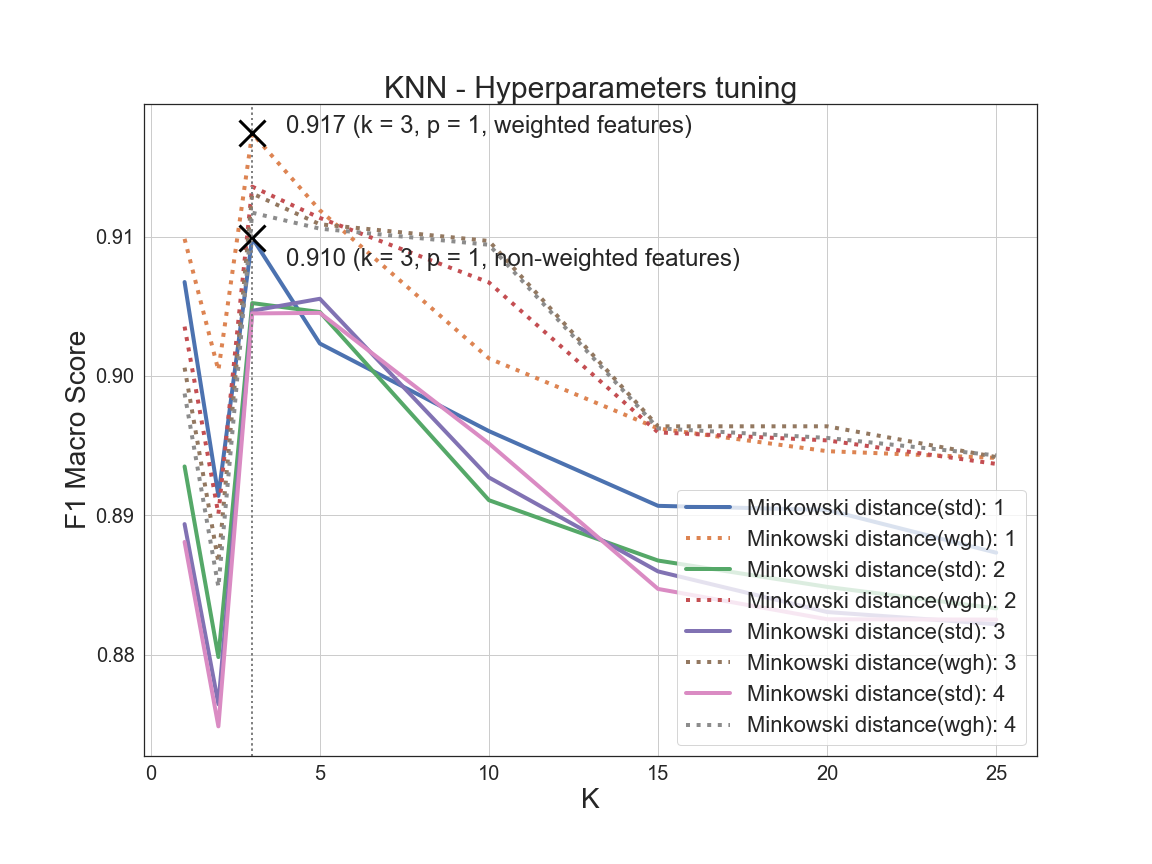
\includegraphics[width=\columnwidth]{chapter5/figure/knn_tuning.png}
	\caption{Hyperparameters p, k tuning, with different weightings}
	\label{fig:knn_tuning}
\end{figure}
The different colours represent the Minkowski distances tested, as well as the different line styles, dotted and continue, represent the weighted and the non-weighted solutions, respectively.

As visible in the picture, the best score, in the usual 10-fold crossvalidation, has been obtained with 5 neighbours, the Manhattan distance, and the weighted solution, which is averagely better than the other one.

The final model has been created with the following call: \textit{KNeighborsClassifier(p=1, n\_neighbors=5)} and it has been fitted with the weighted data, obtaining the following scores in 10-fold-crossvalidation:

\begin{itemize}
	\item[\PencilRight] \textit{Precision}: \textbf{0.924}
	\item[\PencilRight] \textit{Recall}: \textbf{0.917}
	\item[\PencilRight] \textit{F1 score}: \textbf{0.918}
\end{itemize}


\subsection{Text-based Naive Bayes classifier}
In chapter \ref{capitolo4} we created some useful features that helped the above-mentioned classifiers . Anyway we didn't consider enough the tweet texts. A first idea consisted in add a feature that describe the context of the tweets. This task was easily viable using \textit{Google Cloud Natural Language}. Unfortunately, this service only provides a few free calls, and we would not be able to tag all the tweets in our dataset. Moreover, the Context Classification is very specific, and we would have risked to have a too large domain of values. We tried to classify some tweets and we noticed that it was not possible with many of them, since they were just exclamations or contextless sentences. We therefore decided to train a proprietary text classifier. This allowed us to classify texts according to our targets, and our final classifier would have been self-sufficient, without external services.
\subsubsection{Dataset}
Since we wanted to classify texts instead of users, we needed to create a specific dataset.
It had to contain a list of tweets and all the related target. We composed it by binding the target of each tweet to the label of its author. This produced some noise; often bots tweet something different from their goal, to seem more humans. We could accept this problem, since most of the tweets are aimed to a goal.
The shape of the dataset is the following:

\begin{center}
	\begin{tabular}{lr}
		category&\# tweets\\
		\hline\hline
		NSFW&196712\\
		news\_spreaders&280300\\
		spam&453719\\
		fake\_followers&41316\\
		genuine&261233\\
		\hline\\\\
	\end{tabular}
\end{center}

It seems unbalanced, anyway it is appropriate to keep all the data. Some spambot's tweets just contain links and they will be removed in the next steps. Differently, Fake-followers usually don't tweet, or they never tweeted.

\subsubsection{Model}
In order to classify texts, we decided to use a Naive Bayes approach. This algorithm consists in a probabilistic classifier based on the Bayes' theorem. ``Numerous researchers proved that it is effective enough to classify the text in many domains \cite{svm}. Naive Bayes models allow each attribute to contribute towards the final decision equally and independently from other attributes`` \cite{nb}.

Tweets can't be processed as they are. Since this model aims to classify texts basing on its words, we had to clean the dataset from all those parts of the text that are not real or useful words. For example articles, smiles, punctuation should not be taken into consideration. Moreover it is fundamental to reduce inflected words to their word stem. Finally, we need to clean all those noisy parts of the tweets, which is important to allow the final text classifier to consider only real words, in order to identify the context.

Tweets without this pre-processing step look like this:\\

\framebox[\textwidth][l]{\parbox{\textwidth}{\textit{'RT @SteveSchmidtSES: TRUMP disgraced the Presidency and the\\United States at the G-7 summit. From his slovenly appearance to his\\unprepared... https://t.co/KiT29FvJw5'}}}\\

In order to perform this tasks, we used a \textit{sklearn Pipeline}. It is a method that allows to build a custom predictive algorithm. In our case, it contains intermediate steps of data transformation and finally the machine learning algorithm. It works like a generic model, but it perform all the included transformations before processing a data, both in training and prediction steps.

We added to the pipeline the following operations:

\begin{itemize}
	\item[\PencilRight] \textbf{Remove retweet information:}\\
	Delete the texual pattern which indicates that the current status is a retweet. It consists in a "RT @original\_author:". 
	\item[\PencilRight] \textbf{Remove punctuation:}\\
	With regular expressions we removed everythink different from characters and numbers. In this step also smiles and other symbols are removed.
	\item[\PencilRight] \textbf{Remove stopwords:}\\
	stopwords are the most common words that are always used in a language and that can not help to classify a context. Some example of words belonging to this category are articles or prepositions.
	We removed them, by using a stopwords dictionary of \textit{NLTK} libraries.
	\item[\PencilRight] \textbf{Transform uppercase characters into lowercase:}\\
	Before tokenize words, we transformed every character into lowercase, in order to be sure that every word is considered only in one form.
	\item[\PencilRight] \textbf{Apply stemming:}\\
	This is the step where words are reduce to their word stem. Since the text classifier is based on the occurrences of words in the texts, we don't need a correct grammar in our tweets. Instead, words at their basic form are more useful for the target.
	In order to perform this transformation we used \textit{SnowballStemmer} from \textit{NLTK} libraries.
	\item[\PencilRight] \textbf{Apply TF-IDF encoding:}\\
	Finally we applied to each word a TF-IDF encoding. Since we had a huge amount of tweets, without this step we would have risked to give too much importance to the overused wordsand almost nothing importance to the others. Moreover, without using TF-IDF we had a worse performance.
	\item[\PencilRight] \textbf{MultinomialNB:}\\
	This is the final classification algorithm. Thanks to the pipeline it always receives cleaned data, performing a better training and predictions.
	We selected a Naive Bayes classifier for multinomial models since we are dealing with a multi-class problem.
\end{itemize}

\subsubsection{Holdout evaluation}
The final text classifier has the following performance:
\begin{itemize}
	\item[\PencilRight] \textit{F1 score:} \textbf{0.71} with TF-IDF
	\item[\PencilRight] \textit{F1 score:} \textbf{0.64} without TF-IDF
\end{itemize}

Since the other models classify users and not single tweets, we could not use a classifier for texts only.
In order to get a prediction on users, based only on their tweets, the final classification script compute the resulted probabilities for each tweet. Then, for each user, the final prediction consists in the mean of the predictions over his tweets.
% !TEX root = ../thesis.tex
\chapter{Bot classifiers}
\label{capitolo5}
\thispagestyle{empty}

In this chapter we will show the choices and stages behind the final model.
Starting from baseline models, we enhanced the chosen classifiers with handcrafted features coming from the last chapter.\\
We saw and studied the performance improvements with validation approaches, and this phase led us to our current solution.

The result involves three models:
\begin{itemize}
	\item[\PencilRight] a first Random Forest classifier that has been used to provide an early filter on the separation between genuine accounts and bots
	\item[\PencilRight] a second Random Forest that gives a classification among the four studied categories of bots only
	\item[\PencilRight] a Naive Bayes classifier, used over the same classes of the second Random Forest, but which reads and labels the users, according on their tweets only
	\item[\PencilRight] a K-Nearest Neighbours classifier, used over the four bot classes, based on the user features only
\end{itemize}
The algorithms were used together into a pipeline work-flow, whose first step is the detection of bots from humans, thanks to the first binary Random Forest.
Then, the percentage of membership in the bot category is further split into four sub-percentages, which represent the prediction over the inner bot categories.
This last partition is performed by a stacking ensemble, whose goal is to combine the predictions of the three multi-class models.


\section{Baselines}
The choices explained in this section were made at the same time of the ones listed in the Baseline section of the last chapter.

This is, basically, the same stage of the above-mentioned, but in a model-driven perspective.
The features involved are the ones described in section \ref{baseline}, but we started from that base, to try different classifiers over it.
We chose to evaluate the performances of raw classifiers, for both the binary and the multi-class problem.
Each type of classifiers has been tested with the respective dataset, but considering only the baseline features of those data.

Furthermore, no parameters tuning has been applied, in order to minimize the results of our baselines classifier, with their standard settings.
\subsection{Random Forest}
Random forest is an ensemble learning method used in classification tasks and prediction ones as well.

The algorithm builds several \textit{decision trees} and the resulting output is provided by the mode of the predictions coming from the estimators in the forest.

Each decision tree is trained on a subset of the original data, formed by sampling with replacements the whole training set. They share the same splitting criterion, in order to build subtrees, which is the entropy:\\
Every tree computes the Information Gain of each feature, which is the difference, in terms of entropy, between the information gained on the data \textit{D}, before splitting on the attribute \textit{X}, and the one gained after the split, which provides \textit{n} subsets of \textit{D}.
\[{ \mathit{InformationGain(X)} = \mathit{Information(D)} - \mathit{Information_{X}(D)}}\]
where
\[{ \mathit{Information(D)} = - p_{1}\log p_{1} - ... - p_{n} \log p_{n}}\]
and
\[{ \mathit{Information_{X}(D)} = \frac{|D_{1}|}{|D|}Information(D_{1}) + ... + \frac{|D_{n}|}{|D|}Information(D_{n}) }\]
The attribute providing the highest InformationGain, against the others at the same level of the tree, is chosen to perform a split.

The feature set considered by each tree is a random subset of the original pool.

Due to its ability to face overfitting and to the feature importance ranking that it can provide, this tool is often preferred over other models belonging to the same category.

The advantage of preventing overfitting usually comes with a slower prediction time, because it needs enough estimators for this task.
But, for our purpose, there were enough estimators to face the variance problem without affecting the generalization speed.
\subsection{Logistic Regression}
Logistic regression is a common statistical model, that uses a sigmoid function to map the output of a linear regression on a normalized score, giving the probability, for each sample, to belong to the positive class, given its features and a weighting vector:
\[{\displaystyle P(\hat{y}_{i} = +1 | \vec{x}_{i}, \vec{w})={\frac {1}{1+e^{-\vec{w}h(\vec{x}_{i})}}}}\]

Where $ \hat{y}_{i} $ is the predicted target, over the  \textit{$i_{th}$} sample, \textit{$ \vec{x}_{i} $} is the feature vector of that sample, \textit{$ \vec{w} $} represents the weighting vector that has to be learned and \textit{h} is the activation function of the linear regression.

Logistic Regression searches for the weighting vector that matches the highest likelihood and, in order to do that, it minimizes a cross-entropy
error function, provided by the negative log of the likelihood:
\[{ \mathbf{L}(\vec{w}) = -\ln \prod\limits_{i=1}^{n} P(\hat{y}_{i} = +1 | \vec{x}_{i}, \vec{w})}\]

In multi-classes tasks, there are two possible approaches to face the problem:
\begin{itemize}
	\item[\PencilRight] a more general \textit{softmax} function to replace the logistic sigmoid, which assigns the probability, for the  \textit{$i_{th}$} sample, to belong to the class \textit{C}:
	\[{\displaystyle P(\mathbf{C}_{i} | \vec{x}_{i}, \vec{w})={\frac {e^{-\vec{w}h(\vec{x}_{i})}}{\sum\limits_{j = 1}^{n}e^{-\vec{w}h(\vec{x}_{j})}}}}\]
	\item[\PencilRight] ``One-vs-Rest`` method, which for each class builds a model that predicts the target class against all the others.
\end{itemize}
We decided to stick with the default settings of the libraries involved, so OvR was the approach used for the baseline.

\subsection{K-Nearest Neighbors}
K-Nearest Neighbors is an instance-based model used for classification, regression and pattern recognition. It is considered as a lazy learning algorithm, because all the computation is deferred until the prediction phase.
When it performs a classification over a new point, it looks for the \textit{K} nearest samples in the training set, according to a chosen metric, and it assigns, to the unseen sample, the mode of the targets of the retrieved neighbors.

The choices to make are the ones regarding the number \textit{K} of neighbors to consider, the weights to assign to them and the metric to calculate the distance with.
We used the default settings for the metric (\textit{Euclidean distance}) and for the weighting technique (\textit{uniform}), but we chose to consider 10 neighbors, because the automatic setting was \textit{K} = 5, which is the number of our possible targets.
We chose a \textit{K} that is large enough to make the model not too sensible to outliers, and restricted enough to sharpen the classes boundaries.

We first normalized the training data and then we fitted the algorithm on them, in order to simplify the distance computations.

\subsection{Support Vector Machine}
Support Vector Machine is a smart way to do instance-based learning. It can be seen as a generalization of the weighted KNN algorithm, with an arbitrary and feasible \textit{kernel function}, instead of the more generic dot product.

It can be summarised with a support vector $ \mathbf{\vec{x}} $ (a subset of the training set), a weighting vector $ \mathbf{\vec{w}} $ for them and a \textbf{kernel} \textit{K(x, x')} (a similarity function).

In order to make it work properly, three choices must be made:
\begin{itemize}
	\item[\PencilRight] a proper kernel, which is often selected according to experience and domain knowledge of the problem. We wanted to make things simple in this stage, so we used the default kernel function, which is the Radial Basis Function:\label{rbf}
	\[ K(x, x') = exp(- \frac{||x-x'||^{2}}{2\sigma^{2}}) \]
	with $ \sigma $ as a free parameter
	\item[\PencilRight] the weights $ \vec{w} $, which are obtained by maximizing the margin that splits the records belonging to different classes. Each samples are mapped into a space, thanks to what is known as the \textit{kernel trick}. The ``trick`` helps a linear classifier to work on a non-linear problem, applying the kernel function in the prediction phase.\\This process highlights the boundary that separates the points belonging to different classes.
	SVM aims to draw the boundary for the classes, in order to maximize the ``margin`` formed between the closest points that have different targets
	\item[\PencilRight] the support vector $ \vec{x} $, which comes as a consequence of choosing weights
\end{itemize}
Since we were still facing a multitarget problem, the binary nature of SVM must had been adapted to our needs. We decided, once again, to stick with the default setting for non-binary classifications, in order to have only raw baselines to compare.

The multi-target classification is handled with ``One-vs-One`` approach.
It considers all possible pairwise binary classifiers and so it leads to $\frac{N(N-1)}{2}$ individual binary classifiers, where N is the number of the classes in the problem.

In comparison with "One-vs-Rest" approach, ``One-vs-One`` is less sensitive to an imbalanced dataset, but it's more computationally expensive then the the other, which only builds N binary classifiers.
Despite our choices over methods and parameters weren't accurate in this stage as they were in the other ones, we decided to stick with this setting for SVM, because otherwise it would have led us to an irrelevant algorithm, in comparison with the above-mentioned.

\subsection{Comparison and baseline selection}
Different tasks imply different evaluation metrics. Every classifier was validated and selected according to certain indices of goodness. In particular, we followed a triple of metrics that involves Precision, Recall and F1, for the multi-class problem and we aimed to maximize AUC score for the binary case.
\subsubsection{Multi-class metric}
The selected baseline models were tested with a holdout approach at first, then with a crossvalidation method.
We built a Confusion Matrix for each model, in order to bring out goodness indices for each class, such as \textit{True Positive} (TP), \textit{False Positive} (FP) and \textit{False Negative} (FN).
The evaluation metrics considered are \textit{Precision}, \textit{Recall} and \textit{F1 score} and they work on the mentioned indices.
\begin{itemize}
	\item[\PencilRight] $ Precision = \frac{TP}{TP+FP} $\\
	It measures the proportion of positive identifications, for a given target, that was actually correct.
	\item[\PencilRight] $ Recall = \frac{TP}{TP+FN} $\\
	It measures the proportion of actual positive classifications that was identified correctly.
	\item[\PencilRight] $ F1 score = \frac{2(Precision \times Recall )}{Precision+Recall} $\\
	It calculates the harmonic mean of the previous metrics.
\end{itemize}
Every metric is adapted to fit a multi-class problem. For each class, it has been computed this set of measures, and then they were averaged without weights (macro average), in order to not take label imbalance into account.

\subsubsection{Binary metric}
Since this classifier was built for a different purpose, with respect to the multi-class models, the \textit{Area Under the Curve} score (AUC) is the metric we followed, both for baselines and the final model evaluation.
Area Under the Curve represents the goodness of a classifier, in terms of the integral of the \textit{Receiver Operating Characteristic} (ROC curve), defined over the variation of a decision treshold.

The ROC curve lies in a bi-dimensional space, which has the \textit{True Positive Ratio} ($ TPR =  \frac{TP}{TP+FN}$) on the Y-axis, and the False Positive Ratio ($ FPR =  \frac{FP}{FP+TN}$ ) on the X-axis.
In general, a classifier should accomplish more than 0.5 in AUC score, because that threshold represents a random guesser, which has the 50\% of probabilities to detect the actual class.
The more the AUC score tends to 1, the better is the ability of the classifier to distinguish among classes.

The motivation behind the adding of this new metric is that we had a balanced binary dataset, and this metric is a good fit for this kind of problem. Moreover, Botometer claims to have accomplished an AUC of 0.95, on a 10-fold crossvalidation test.
We wanted to get close to that score, using our crafted features.


\subsection{Holdout evaluation}
The holdout evaluation is performed separating the samples in the dataset into training and test subsets. The splitting process is randomized and it requires a bigger portion of the original dataset to be inserted in the training data, comparing to the amount of samples that will form the test set. A common choice is to use a third of the data to evaluate the model.

\subsection{Multi-class}
In this case, we decided to use 75\% of the data for the training set and 25\% for the test set. This choice is a little bit different from the most common one, which builds the training set with 2/3 of the whole data, because we didn't dispose of a huge amount of records, so we preferred this ratio and then trying an other validation method for comparison.
Here we list the algorithms and their parameters, as they were written according to the Scikit-learn library for Python, their confusion matrix and their scores:
\begin{itemize}
	\item[\PencilRight] \textit{RandomForestClassifier(n\_estimators = 10, criterion = 'entropy')}\\
	Confusion matrix:
	
	{
		\centering
		\begin{tabular}{@{}cc|cccc@{}}
			\multicolumn{1}{c}{} &\multicolumn{1}{c}{} &\multicolumn{4}{c}{Predicted class} \\ 
			\multicolumn{1}{c}{} & 
			\multicolumn{1}{c|}{} & 
			\multicolumn{1}{c}{NSFW} & 
			\multicolumn{1}{c}{NS} &
			\multicolumn{1}{c}{SB} & 
			\multicolumn{1}{c}{FF} \\
			\cline{2-6}
			\multirow[c]{4}{*}{\rotatebox[origin=tr]{90}{Actual class}}
			& NSFW  & 1690 & 27 & 12 & 6\\
			& NS  & 27  & 785 & 30 &  0\\
			& SB  & 14  & 39 & 1280 & 5\\
			& FF  & 12 &  7 &  18 & 1215\\
			\cline{2-6}\\
		\end{tabular}\\
	}
	
	Precision: 0.957\\
	Recall: 0.958\\
	F1 score: 0.957

	\item[\PencilRight] \textit{LogisticRegression(fit\_intercept=True, max\_iter=100, penalty='l2')}\\
	Confusion matrix:
	
	{
		\centering
		\begin{tabular}{@{}cc|cccc@{}}
			\multicolumn{1}{c}{} &\multicolumn{1}{c}{} &\multicolumn{4}{c}{Predicted class} \\ 
			\multicolumn{1}{c}{} & 
			\multicolumn{1}{c|}{} & 
			\multicolumn{1}{c}{NSFW} & 
			\multicolumn{1}{c}{NS} &
			\multicolumn{1}{c}{SB} & 
			\multicolumn{1}{c}{FF} \\
			\cline{2-6}
			\multirow[c]{4}{*}{\rotatebox[origin=tr]{90}{Actual class}}
			& NSFW  & 1274 & 213 & 197 & 51\\
			& NS  & 24 & 740 & 75 & 3\\
			& SB  & 29 & 87 & 1144 & 78\\
			& FF  & 204 &  49 &  46 & 953\\
			\cline{2-6}\\
		\end{tabular}\\
	}
	
	Precision: 0.793\\
	Recall: 0.807\\
	F1 score: 0.794
	
	\item[\PencilRight] \textit{KNeighborsClassifier(n\_neighbors=10)}\\
	Confusion matrix:
	
	{
		\centering
		\begin{tabular}{@{}cc|cccc@{}}
			\multicolumn{1}{c}{} &\multicolumn{1}{c}{} &\multicolumn{4}{c}{Predicted class} \\ 
			\multicolumn{1}{c}{} & 
			\multicolumn{1}{c|}{} & 
			\multicolumn{1}{c}{NSFW} & 
			\multicolumn{1}{c}{NS} &
			\multicolumn{1}{c}{SB} & 
			\multicolumn{1}{c}{FF} \\
			\cline{2-6}
			\multirow[c]{4}{*}{\rotatebox[origin=tr]{90}{Actual class}}
			& NSFW  & 1578 & 36 & 60 & 61\\
			& NS  & 81 & 685 & 63 & 13\\
			& SB  & 81 & 32 & 1187 & 38\\
			& FF  & 104 & 6 & 55 & 1087\\
			\cline{2-6}\\
		\end{tabular}\\
	}
	
	Precision: 0.883\\
	Recall: 0.869\\
	F1 score: 0.875
	
	\item[\PencilRight] \textit{SVC(kernel='rbf', decision\_function\_shape='ovo')}\\
	Confusion matrix:
	
	{
		\centering
		\begin{tabular}{@{}cc|ccc@{}}
			\multicolumn{1}{c}{} &\multicolumn{1}{c}{} &\multicolumn{3}{c}{Predicted class} \\ 
			\multicolumn{1}{c}{} & 
			\multicolumn{1}{c|}{} & 
			\multicolumn{1}{c}{NSFW} & 
			\multicolumn{1}{c}{SB} & 
			\multicolumn{1}{c}{FF} \\
			\cline{2-5}
			\multirow[c]{3}{*}{\rotatebox[origin=tr]{90}{Actual class}}
			& NSFW  & 1735 & 0 & 0\\
			& NS  & 842 & 0 & 0\\
			& SB  & 1114 & 223 & 1\\
			& FF  & 483 & 0 & 769\\
			\cline{2-5}\\
		\end{tabular}\\
	}
	
	Precision: 0.603\\
	Recall: 0.445\\
	F1 score: 0.408
	
\end{itemize}

From these evaluations it is possible to see how the Random Forest algorithm outperforms Logistic Regression and Support Vector Machine. This difference colud be driven by the multi-class task. Logistic Regression and SVM need to be adapted to this purpose. Another factor that can discriminate the performances is the choices of the features and their magnitude. Random Forest doesn't require attribute normalization to top its scores, additionally, every feature has been ranked and tested with the inner feature ranking provided by the algorithm. It is possible that some of these attributes need further processing to better support the other models tested.


\subsubsection{Binary}
This evaluation was made with the common splitting ration between train and test set. Since we had 31,212 samples available, well balanced, we used two thirds (20,808) for the training set and the remaining (10,404) for the test set.
We wanted a first term of comparison, so, in the beginning, we evaluated the AUC metric with the holdout technique.
\begin{itemize}
	\item[\PencilRight] \textit{RandomForestClassifier(n\_estimators = 10, criterion = 'entropy')}\\
	Confusion matrix:
	
	{
		\centering
		\begin{tabular}{@{}cc|cc@{}}
			\multicolumn{1}{c}{} &\multicolumn{1}{c}{} &\multicolumn{2}{c}{Predicted class} \\ 
			\multicolumn{1}{c}{} & 
			\multicolumn{1}{c|}{} & 
			\multicolumn{1}{c}{BOT} & 
			\multicolumn{1}{c}{GEN}  \\
			\cline{2-4}
			\multirow[c]{2}{*}{Actual class}
			& BOT  & 4314 & 336\\
			& GEN  & 554 & 4160\\
			\cline{2-4}
			\multicolumn{2}{r|}{AUC} & 
			\multicolumn{2}{l}{0.905}\\
		\end{tabular}\\
	}

	\item[\PencilRight] \textit{LogisticRegression(fit\_intercept=True, max\_iter=100, penalty='l2')}\\
	Confusion matrix:
	
	{
		\centering
		\begin{tabular}{@{}cc|cc@{}}
			\multicolumn{1}{c}{} &\multicolumn{1}{c}{} &\multicolumn{2}{c}{Predicted class} \\ 
			\multicolumn{1}{c}{} & 
			\multicolumn{1}{c|}{} & 
			\multicolumn{1}{c}{BOT} & 
			\multicolumn{1}{c}{GEN}  \\
			\cline{2-4}
			\multirow[c]{2}{*}{Actual class}
			& BOT  & 3124 & 1526\\
			& GEN  & 558 & 4156\\
			\cline{2-4}
			\multicolumn{2}{r|}{AUC} & 
			\multicolumn{2}{l}{0.776}\\
		\end{tabular}\\
	}

	
	\item[\PencilRight] \textit{KNeighborsClassifier(n\_neighbors=10)}\\
	Confusion matrix:
	
	{
		\centering
		\begin{tabular}{@{}cc|cc@{}}
			\multicolumn{1}{c}{} &\multicolumn{1}{c}{} &\multicolumn{2}{c}{Predicted class} \\ 
			\multicolumn{1}{c}{} & 
			\multicolumn{1}{c|}{} & 
			\multicolumn{1}{c}{BOT} & 
			\multicolumn{1}{c}{GEN}  \\
			\cline{2-4}
			\multirow[c]{2}{*}{Actual class}
			& BOT  & 3698 &  952\\
			& GEN  & 1129 & 3585\\
			\cline{2-4}
			\multicolumn{2}{r|}{AUC} & 
			\multicolumn{2}{l}{0.777}\\
		\end{tabular}\\
	}

	
	\item[\PencilRight] \textit{SVC(kernel='rbf')}\\
	Confusion matrix:
	
	{
		\centering
		\begin{tabular}{@{}cc|cc@{}}
			\multicolumn{1}{c}{} &\multicolumn{1}{c}{} &\multicolumn{2}{c}{Predicted class} \\ 
			\multicolumn{1}{c}{} & 
			\multicolumn{1}{c|}{} & 
			\multicolumn{1}{c}{BOT} & 
			\multicolumn{1}{c}{GEN}  \\
			\cline{2-4}
			\multirow[c]{2}{*}{Actual class}
			& BOT  & 4625 & 25\\
			& GEN  & 4676 & 38\\
			\cline{2-4}
			\multicolumn{2}{r|}{AUC} & 
			\multicolumn{2}{l}{0.501}\\
		\end{tabular}\\
	}

\end{itemize}

Once again, Random Forest has the best scores, even in the binary problem. Although, e can see a worsening in the KNN performances in this test. It can be imputable to an ``unlucky`` holdout set or to the fixed parameters tested.

\subsection{Crossvalidation}
This approach is based on repeated holdouts. It is performed by splitting the whole data in \textit{K} non-overlapping folds, leading to \textit{K} different holdout evaluations. The results for each step are stored and the final evaluation is given by the mean of the \textit{K} evaluations. For each evaluation, one fold is used for testing, the other ones for training the models. A common practice is to set \textit{K = 10} and thus averaging 10 different evaluations.
This method is also known as \textit{K-fold crossvalidation}. We used a stratified approach, which takes care about keeping the labels balanced on each fold.

Due the need of performing ten steps, it is computationally more expensive then a simple holdout validation. In our case, it was feasible, in term of speed, because of the models complexity and the data amount. This situation held for both the binary and the mutliclass tasks.

The obtained scores are also more meaningful, with regards to holdout, because they are less sensitive to ``lucky`` or ``unlucky`` splits.

Here is the results for every baseline model:
\subsubsection{Multi-class}
\begin{itemize}
	\item[\PencilRight] \textit{RandomForestClassifier(n\_estimators = 10, criterion = 'entropy')}\\
	Mean precision: 0.947\\
	Mean recall: 0.945\\
	Mean f1 score: 0.943
	\item[\PencilRight]\textit{LogisticRegression(fit\_intercept=True, max\_iter=100, penalty='l2')}\\
	Mean precision: 0.827\\
	Mean recall: 0.815\\
	Mean f1 score: 0.815
	\item[\PencilRight]\textit{KNeighborsClassifier(n\_neighbors=10)}\\
	Mean precision: 0.878\\
	Mean recall: 0.858\\
	Mean f1 score: 0.862
	\item[\PencilRight]\textit{SVC(kernel='rbf', decision\_function\_shape='ovo')}\\
	Mean precision: 0.573\\
	Mean recall: 0.456\\
	Mean f1 score: 0.413
\end{itemize}

As the results show, the Random Forest algorithm is the one that achieves the best performances, even with default settings, on both holdout and 10-fold crossvalidation. We thus decided to consider it as the main tool to build our bot categories classifier. 
\subsubsection{Binary}
\begin{itemize}
	\item[\PencilRight] \textit{RandomForestClassifier(n\_estimators = 10, criterion = 'entropy')}\\
	Mean AUC: 0.916\\
	\item[\PencilRight]\textit{LogisticRegression(fit\_intercept=True, max\_iter=100, penalty='l2')}\\
	Mean AUC: 0.792\\
	\item[\PencilRight]\textit{KNeighborsClassifier(n\_neighbors=10)}\\
	Mean AUC: 0.835\\
	Mean precision: 0.779\\
	\item[\PencilRight]\textit{SVC(kernel='rbf')}\\
	Mean AUC: 0.583\\
\end{itemize}
Even in the binary cases, the Random Forest had the best performance, and it could be imputed to the similar features involved in both problems. Moreover, we could see that the Support Vector Machine emerged as a lightly improved random guesser.


\section{Binary Classifier}
Since our dataset was pretty balanced and we couldn't retrieve many more genuine accounts, we didn't want our instrument to treat this category of users just as one the other bot kinds. It was important to perform a previous filter that was able to give importance to the separation between bots and genuine accounts.

We were inspired by the work made with Botometer \cite{Botometer}, which involved a binary labelled dataset, with bot and genuine accounts.
The researchers built their features, grouped them in six main categories, then they ran a Random Forest algorithm per group.

We already had our feature engineering done, so we decided to test it on this new task.

In order to not to build a poorer version of our multi-class model, we didn't want to use a reduced copy of our dataset, stratifying it by stripping random bots from it. We needed a balanced dataset, with about the same amount of genuines and bots. So, we started from the same dataset used by the Botometer project, in order to have a baseline comparison.
\subsection{Dataset}
The dataset we used for this classification was composed of part of our collected records and of some entries from the Caverlee-2011 dataset, which contains 22,223 content polluters and 19,276 legitimate users, both collected through a social honeypot, as described in their paper \cite{Lee11sevenmonths}.

We used the APIs to retrieve the ids for both genuines and bots, from the Caverlee list. The process provided us 15,687 legitimate user ids, and 15,525 general bot ids (without inner classifications), for a total number of 31,212 samples.
The difference from the original number of entries is due to the age of the dataset. Since 2011, the year of the creation of the list, a lot of accounts have been deleted or suspended.

The feature vector we used is the same that came out from the feature engineering process, except for the specific characterizing features, that weren't considered, because crafted for the inner separation among bots. We excluded the \textit{NSFW\_avg}) image feature, as we noticed it didn't bring much performance boosting with the multi-class models.
The extrinsic features must had been adjusted with new dictionaries, so we had two features: (\textit{bots\_words\_score} and  \textit{genuine\_words\_score}.
Both the features have been computed as for the multi-class case, with up to 1000 non overlapping words in each dictionary.

\subsection{Model}
The model chosen for the purpose was the best performer of the tested baselines: the Random Forest binary classifier.
The algorithm has had its parameters tuned during the validation phase.
We decided to stick with 10-fold crossvalidation, as it was done for the baselines.

After several Grid Search runs, the last round computed had this hyperparameters to combine together:
\begin{itemize}
	\item[\PencilRight] \textit{n\_estimators} = [150, 200, 250, 300, 350, 400, 450, 500]
	\item[\PencilRight]\textit{max\_depth} = [None, 26, 28]
	\item[\PencilRight]\textit{criterion} = 'entropy'
\end{itemize}
\begin{figure}[htp!]
	\centering
	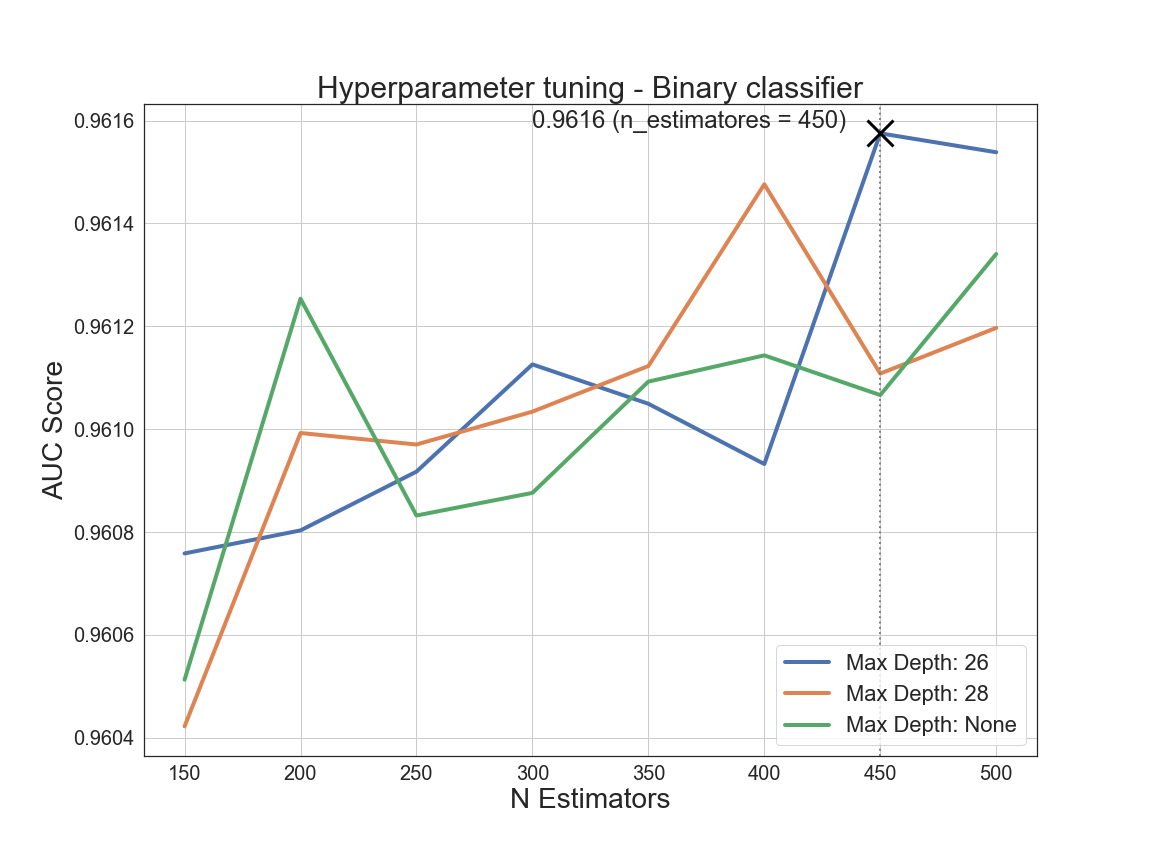
\includegraphics[width=\columnwidth]{chapter5/figure/bon_tuning.png}
	\caption{Grid search results}
	\label{fig:grid_search}
\end{figure}
\begin{figure}[htp!]
	\centering
	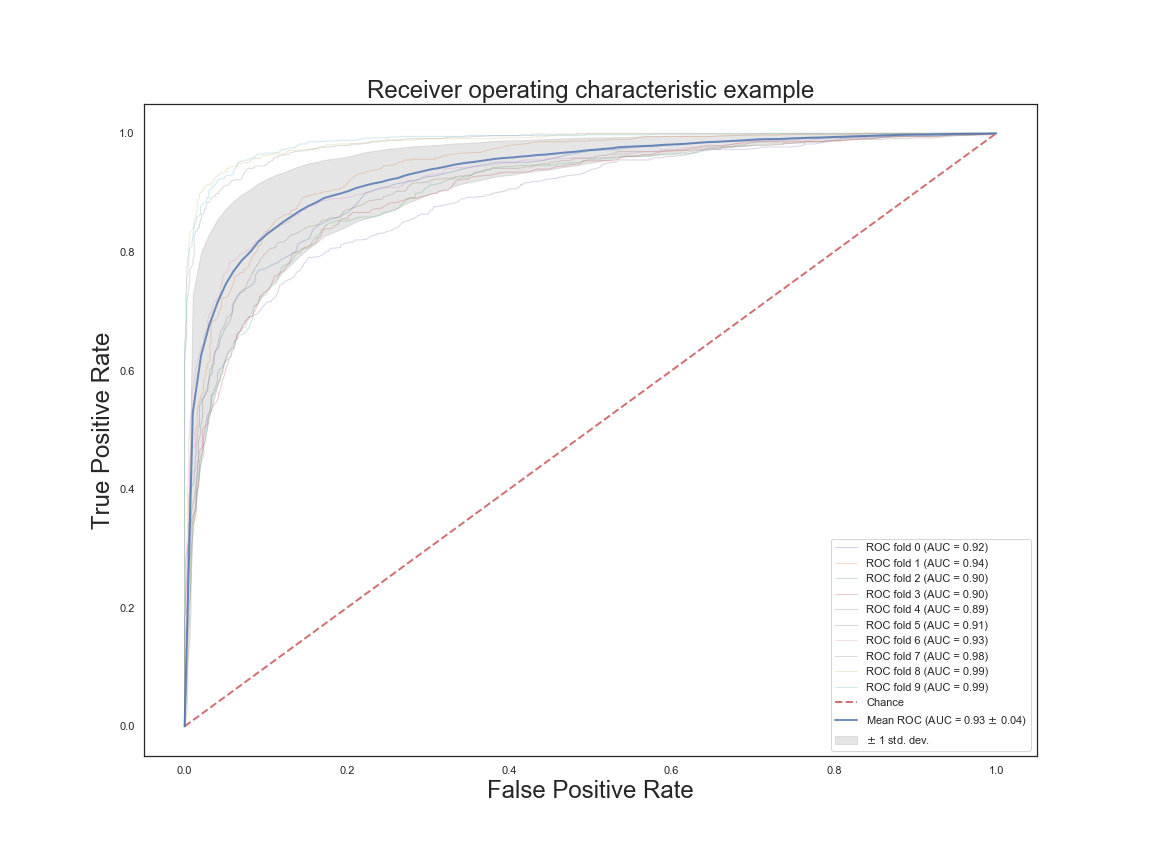
\includegraphics[width=\columnwidth]{chapter5/figure/auc.png}
	\caption{ROC curve}
	\label{fig:auc}
\end{figure}
As we can see in Figure \ref{fig:grid_search}, the AUC is increasing with the number of the estimators in the forest. We decided t stop at 450, which corresponds to the highest AUC score, since this phase was aimed to find a comparison term with Botometer, but it didn't represent the final model.
In their paper \cite{Varol}, the Botometer group claims to reach 0.95 in AUC score.

The AUC obtained with our arrangement is equal to 0.96, as shown in Figure \ref{fig:auc}, which is a positive accomplishment, considering that it will be used only as support for the identification of humans among bots, but we didn't crafted specific features as the ones involved in the Botometer project and we didn't have the same amount of data neither.

The model has then been fitted with the hole data, with this settings: \textit{ n\_estimators} = 450, \textit{max\_depth} = 26 and \textit{criterion} = 'entropy'.

\subsection{Validation}

We had an interesting amount of data that were not involved in this task, because of the comparison with the same Botometer's dataset. Since this unseen data had a further discrimination among bots, it was easy to sample some records randomly, replacing their multi-class targets with binary values.
We performed this job to validate the newborn model on unseen and fresher data.
We were interested in testing a model that were trained over ``old`` accounts, with consequent different attributes values and different behaviours on the platform, with younger accounts.

This validations would had given us a preview of the real performance of the model, once it would had been deployed on the internet. The account that a user would test with our application could be younger than the ones included in the Caverlee's list.

We sampled 6,000 accounts, divided in 3,000 genuine and 3,000 bot ids, randomly picked by our multi-class dataset.

The binary model were fitted with its data and it was ready to perform new predictions.

Looking at the most relevant features for the classifier, as shown in Figure \ref{fig:bon_importances}, we could find the \textbf{age} field at the top position.

\begin{figure}[htp!]
	\centering
	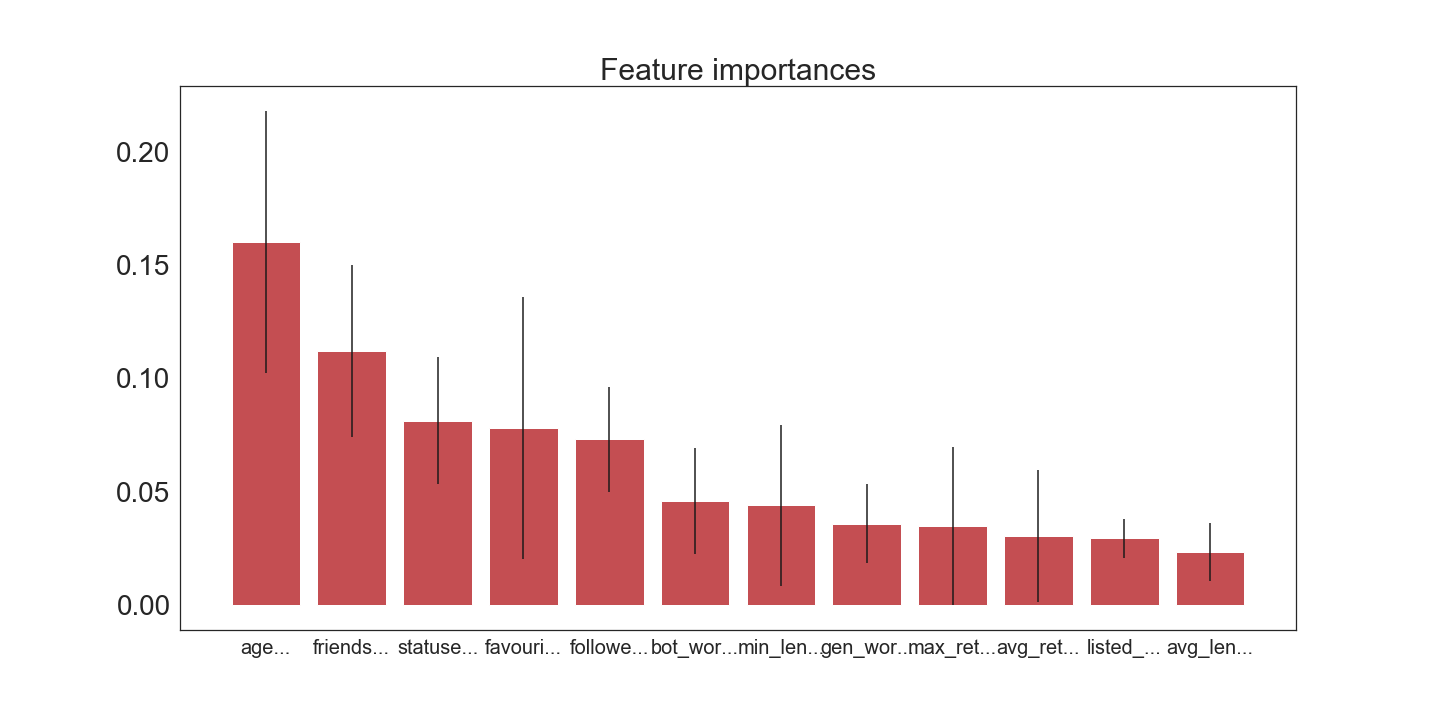
\includegraphics[width=\columnwidth]{chapter5/figure/bon_importances.png}
	\caption{Binary Random Forest features ranking}
	\label{fig:bon_importances}
\end{figure}

This was the first warning of a validation performance worsening.
A said before, the age of the accounts in the Caverlee's dataset were higher than the ones in our dataset. In particular, we examined the \textit{age} field of the training set, and the one coming from our validation samples, picked from the mutliclass dataset.
\begin{table}[!htb]
	\caption{Age field comparison among bot accounts}
	\begin{center}
		\begin{tabular}{@{}lr@{}}
			\multicolumn{2}{c}{\textbf{Training Bots}}\\
			\hline\hline
			\multicolumn{2}{c}{\textit{age}}\\
			\hline
			\multicolumn{1}{l}{mean}& \multicolumn{1}{r}{8}\\
			\multicolumn{1}{l}{std}& \multicolumn{1}{r}{0.66}\\
			\multicolumn{1}{l}{min}& \multicolumn{1}{r}{4}\\
			\multicolumn{1}{l}{max}& \multicolumn{1}{r}{12}\\
			\multicolumn{1}{l}{25\%}& \multicolumn{1}{r}{8}\\
			\multicolumn{1}{l}{50\%}& \multicolumn{1}{r}{9}\\
			\multicolumn{1}{l}{75\%}& \multicolumn{1}{r}{9}\\
			\hline\hline
		\end{tabular}
		\begin{tabular}{@{}lr@{}}
			\multicolumn{2}{c}{\textbf{Validation Bots}}\\
			\hline\hline
			\multicolumn{2}{c}{\textit{age}}\\
			\hline
			\multicolumn{1}{l}{mean}& \multicolumn{1}{r}{4.50}\\
			\multicolumn{1}{l}{std}& \multicolumn{1}{r}{2.69}\\
			\multicolumn{1}{l}{min}& \multicolumn{1}{r}{0}\\
			\multicolumn{1}{l}{max}& \multicolumn{1}{r}{11}\\
			\multicolumn{1}{l}{25\%}& \multicolumn{1}{r}{3}\\
			\multicolumn{1}{l}{50\%}& \multicolumn{1}{r}{4}\\
			\multicolumn{1}{l}{75\%}& \multicolumn{1}{r}{6}\\
			\hline\hline
		\end{tabular}
	\end{center}
	\label{table:bots}
\end{table}


\begin{table}[!htb]
	\caption{Age field comparison among genuine accounts}
	\begin{center}
		\begin{tabular}{@{}lr@{}}
			\multicolumn{2}{c}{\textbf{Training Genuine}}\\
			\hline\hline
			\multicolumn{2}{c}{\textit{age}}\\
			\hline
			\multicolumn{1}{l}{mean}& \multicolumn{1}{r}{9.22}\\
			\multicolumn{1}{l}{std}& \multicolumn{1}{r}{0.54}\\
			\multicolumn{1}{l}{min}& \multicolumn{1}{r}{4}\\
			\multicolumn{1}{l}{max}& \multicolumn{1}{r}{12}\\
			\multicolumn{1}{l}{25\%}& \multicolumn{1}{r}{9}\\
			\multicolumn{1}{l}{50\%}& \multicolumn{1}{r}{9}\\
			\multicolumn{1}{l}{75\%}& \multicolumn{1}{r}{9}\\
			\hline\hline
		\end{tabular}
		\begin{tabular}{@{}lr@{}}
			\multicolumn{2}{c}{\textbf{Validation Genuine}}\\
			\hline\hline
			\multicolumn{2}{c}{\textit{age}}\\
			\hline
			\multicolumn{1}{l}{mean}& \multicolumn{1}{r}{6.40}\\
			\multicolumn{1}{l}{std}& \multicolumn{1}{r}{1.94}\\
			\multicolumn{1}{l}{min}& \multicolumn{1}{r}{3}\\
			\multicolumn{1}{l}{max}& \multicolumn{1}{r}{11}\\
			\multicolumn{1}{l}{25\%}& \multicolumn{1}{r}{5}\\
			\multicolumn{1}{l}{50\%}& \multicolumn{1}{r}{6}\\
			\multicolumn{1}{l}{75\%}& \multicolumn{1}{r}{8}\\
			\hline\hline
		\end{tabular}
	\end{center}
	\label{table:genuine}
\end{table}

Like Tables \ref{table:bots} and \ref{table:genuine} show, there is a clear differences in the age attribute, between training and validation set.

We went forward to check if this diversity would had led us to a bad validation performance, or if the model would had handled the predictions in other ways.

The 10-fold crossvalidation on the validation set produced the following confusion matrix, with the correlated AUC score:\\

{
	\centering
	\begin{tabular}{@{}cc|cc@{}}
		\multicolumn{1}{c}{} &\multicolumn{1}{c}{} &\multicolumn{2}{c}{Predicted class} \\ 
		\multicolumn{1}{c}{} & 
		\multicolumn{1}{c|}{} & 
		\multicolumn{1}{c}{BOT} & 
		\multicolumn{1}{c}{GEN}  \\
		\cline{2-4}
		\multirow[c]{2}{*}{Actual class}
		& BOT  & 558 & 2442\\
		& GEN  & 158 & 2842\\
		\cline{2-4}
		\multicolumn{2}{r|}{AUC} & 
		\multicolumn{2}{l}{0.566}\\
		\multicolumn{4}{c}{}\\
	\end{tabular}\\
}
The worsening were real, and it highlighted the short-sighted training phase we performed, trying to top the Botometer performance.

We tried to mitigate this performance loss, by excluding the main suspect from the features set.
Here is the validation performance, without considering the accounts' ages.

{
\centering
\begin{tabular}{@{}cc|cc@{}}
	\multicolumn{1}{c}{} &\multicolumn{1}{c}{} &\multicolumn{2}{c}{Predicted class} \\ 
	\multicolumn{1}{c}{} & 
	\multicolumn{1}{c|}{} & 
	\multicolumn{1}{c}{BOT} & 
	\multicolumn{1}{c}{GEN}  \\
	\cline{2-4}
	\multirow[c]{2}{*}{Actual class}
	& BOT  & 2920 & 20\\
	& GEN  & 1589 & 1411\\
	\cline{2-4}
	\multicolumn{2}{r|}{AUC} & 
	\multicolumn{2}{l}{0.721}\\
	\multicolumn{4}{c}{}\\
\end{tabular}\\
}

The improvement was encouraging, but still not enough to rely on this basic solution.
Considering the bot target as the positive class, we still had too many False Positive in our confusion Matrix. The binary classifier used to tend to identify an user as a bot, with too much confidence. We had to reduce that number, in order to provide a reliable filter in the final prediction pipeline system.

\subsection{Data extension}
The idea we had was to use some data from our multi-class dataset to enrich the binary training set, in order to make the algorithm handle younger and different types of samples from the Twitter population.

In order to perform the extension, we sampled 3,000 genuine accounts and 8,000 bots (2,000 content polluters for each class), all coming from our dataset, and added them to the Caverlee's dataset.
The new training set was composed by 42,212 samples.

We performed a 10-fold-crossvalidation to see the effect of this data refill, sticking to the same hyperparameters found by the last Grid Search. The AUC score measured with these data was 0.963. We could see a slight improvement of the performances, with this data extension. However, we wanted to take a look inside the inner ranking performed by the algorithm, to check if the age field represented an important splitting point.
Figure \ref{fig:bon_importances_ext} shows that the age attribute was still the most considered when the trees had to perform the first splits.

We couldn't blindly follow the AUC score through Grid Searches, without making considerations about what will happen when we will allow people to classify data coming from outside our collected samples.
The age feature would have driven the Random Forest to misclassification over accounts with low \textit{age} values.
Even if the exclusion of that attribute would had made the overall AUC score worse, we had to strip it from the features vector, in order to better generalize on real test cases.

\begin{figure}[htp!]
	\centering
	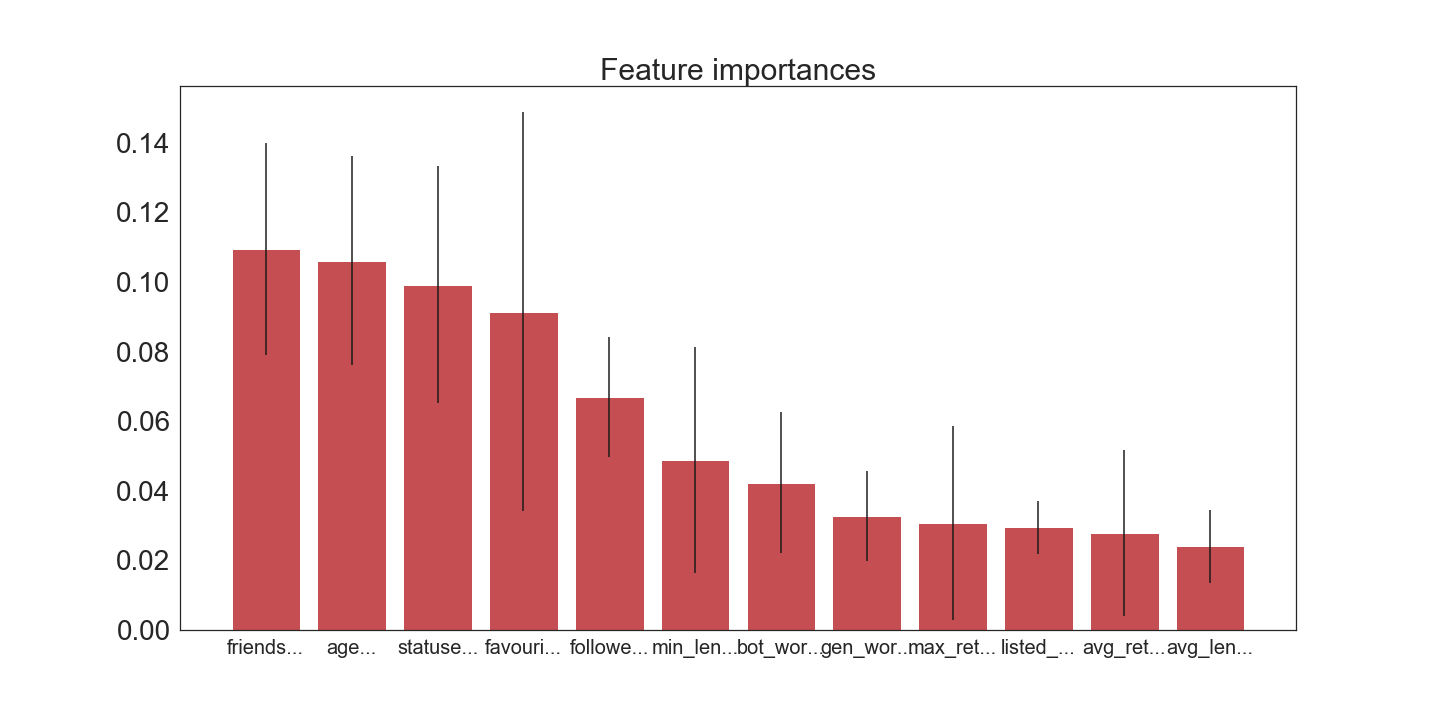
\includegraphics[width=\columnwidth]{chapter5/figure/bon_importances_extensions.png}
	\caption{Features ranking with augmented data - Top 12 }
	\label{fig:bon_importances_ext}
\end{figure}

While cross-validating the model, we tested the complete features vector (with and without the extension from our dataset) and the one stripped by the age values. The crossvalidation was performed with the same hyperparameters settings of the model fitted with the Caverlee's dataset only.

{
	\centering
	\begin{tabular}{@{}cccc@{}}
		\multicolumn{1}{c}{} & 
		\multicolumn{3}{c}{Fitted data} \\ 
		\cline{2-4}
		\multicolumn{1}{c|}{} & 
		\multicolumn{1}{c|}{original - with \textit{age} } & 
		\multicolumn{1}{c|}{extended - with \textit{age} } & 
		\multicolumn{1}{c|}{extended - without \textit{age}} \\
		\cline{1-4}
		\multicolumn{1}{|c|}{AUC} & 
		\multicolumn{1}{c|}{\textbf{0.961}} & 
		\multicolumn{1}{c|}{\textbf{0.963}} & 
		\multicolumn{1}{c|}{\textbf{0.948}} \\
		\cline{1-4}\\
	\end{tabular}\\
}

The age filed removing made thing worse, but we decided to perform it anyway, because of the good score reached without it, and the flexibility we were giving to the Random Forest. The slight worsening could be also imputed to the biased extrinsic features of that data: those samples came from the multi-class dataset and they originally had the extrinsic features based on the four bot categories' dictionaries.
In order to refill the binary dataset with these new samples, we had to recompute the extrinsic features, applying the analogous method used for the binary purpose.
We didn't recompute the entire dictionaries, we just assigned the scores to the new samples we were introducing, basing the calculations on the already listed words. Those had been exposed in chapter \ref{capitolo4}. This approach aimed to force the algorithm to identify bots and humans, basing its comparisons on the online computations of those features, like in a real-case generalization.

This last configuration was used to performed a further tuning of the parameters.
A new Grid Search brought us the configuration for the hyperparameters shown in Figure \ref{fig:bon_tuning_refil}, leading to the new AUC score, exposed in Figure \ref{fig:bon_refil_auc}.
\begin{figure}[htp!]
	\centering
	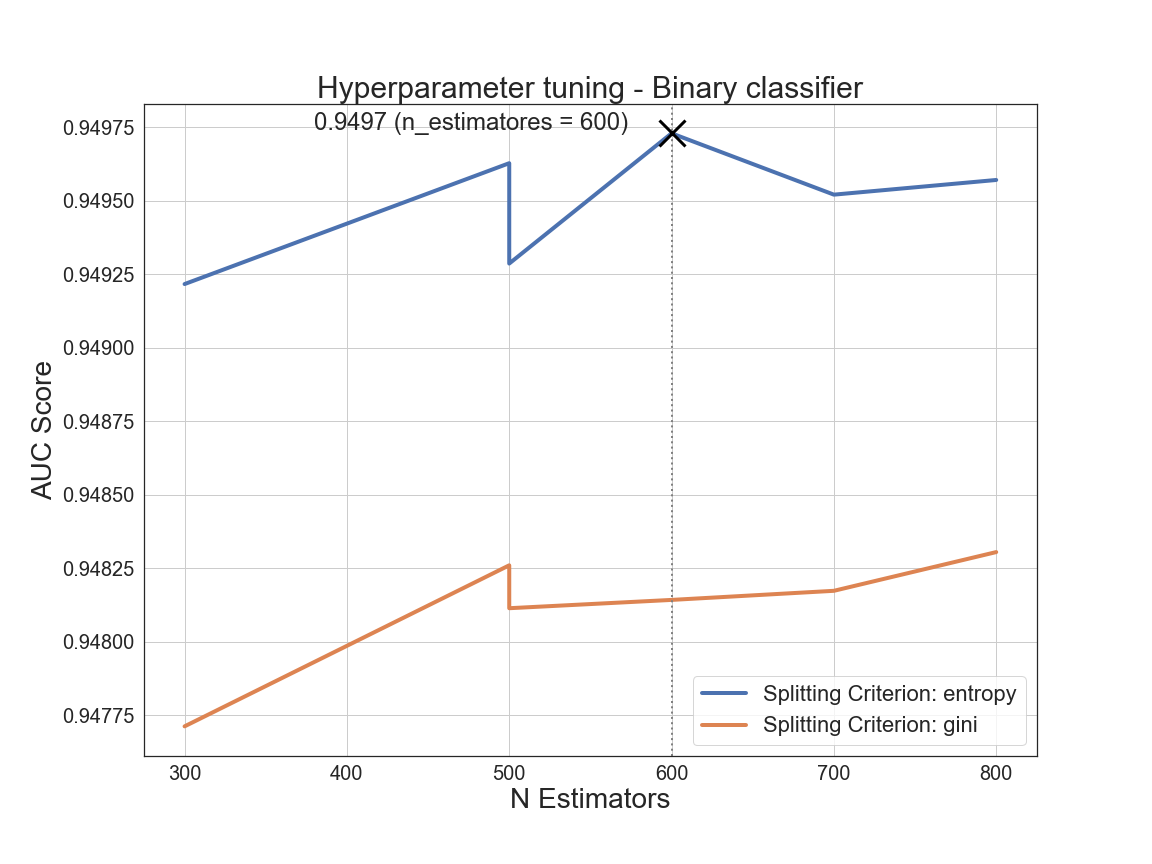
\includegraphics[width=\columnwidth]{chapter5/figure/bon_tuning_refill.png}
	\caption{Grid Search with extended data}
	\label{fig:bon_tuning_refil}
\end{figure}
\begin{figure}[htp!]
	\centering
	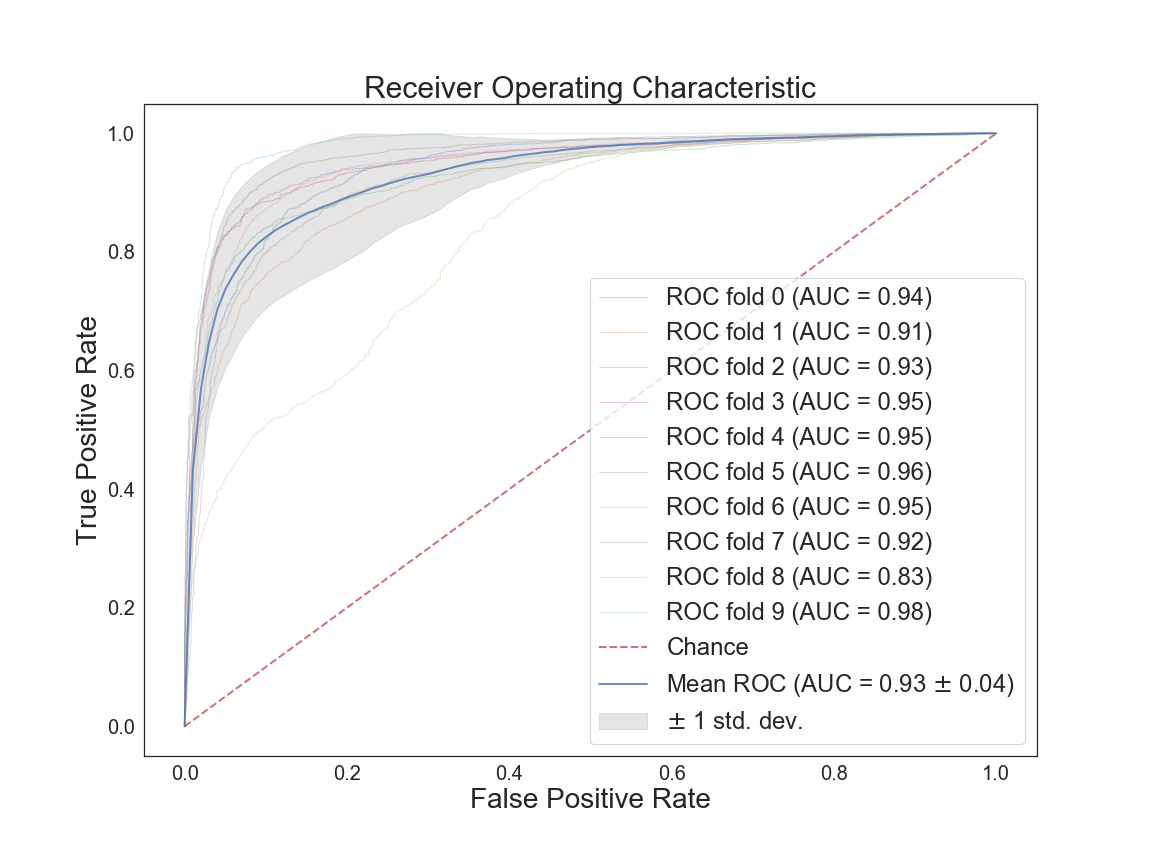
\includegraphics[width=\columnwidth]{chapter5/figure/refill_auc.png}
	\caption{AUC score with extended data}
	\label{fig:bon_refil_auc}
\end{figure}
The binary classifier has then been fitted with 42,212 samples with 34 features, 600 estimators, entropy splitting criterion and 26 levels of maximum depth.

\section{Multi-class ensemble classifier}
It somehow represents the core of our thesis, it models the starting idea: go deep inside bot identification and search and classify similar behaviours among them.

In this section we will expose the model involved in the multi-class ensemble. In this process, we used a Random Forest algorithm, working on all the crafted features; a KNN model, operating on the user attributes only; a final text-based Naive Bayes classifier, which reads the tweets' texts and classifies them.

At first, this ensemble of these three models should have been blended with the prediction of the binary classifier. That means that the genuine class was part of the labels we were trying to classify, even in the multi-class models. Then, we found an issue in this approach: the binary classifier itself wasn't enough, even including it into the ensemble, to give the right importance to the genuine accounts. This problem emerged because of the others classifiers, as they were trying to classify the genuine class too. They lacked in data with that target, so, basically, they used to treat that category as one other of the bot types.

Even if the results on our validation sets were still good (we accomplished a F1 measure of 0.973), for the final ensemble method, we knew that this method would had yielded to a poor bot vs genuine detection tool. We couldn't accept that situation, because, in order to go deeper than other works, in bot behaviour classifications, we had to provide a solid previous discrimination between humans and automated accounts.

The ensemble method with all the classifiers blended together were replaced with a pipeline, and the multi-class models were trained on bot categories only.
These last classifiers had been put together inside a  ensemble, which returns the final mutliclass probability prediction, based on the opinions of those models, as shown in Figure \ref{fig:stacking_schema}

The different nature of the classifiers, and the feature subsets as well, is one of the strengths of the stacking approach: it combines different opinions about the samples, driven by different classifiers, considering different parameters and attributes; basing on those unlike classifications, it builds its own.

It differs from other ensemble methods as bagging and boosting, because of this miscellaneous schema, and it can be a robust method to exploit the different characteristics of the classifiers stacked together.

\begin{figure}[htp!]
	\centering
	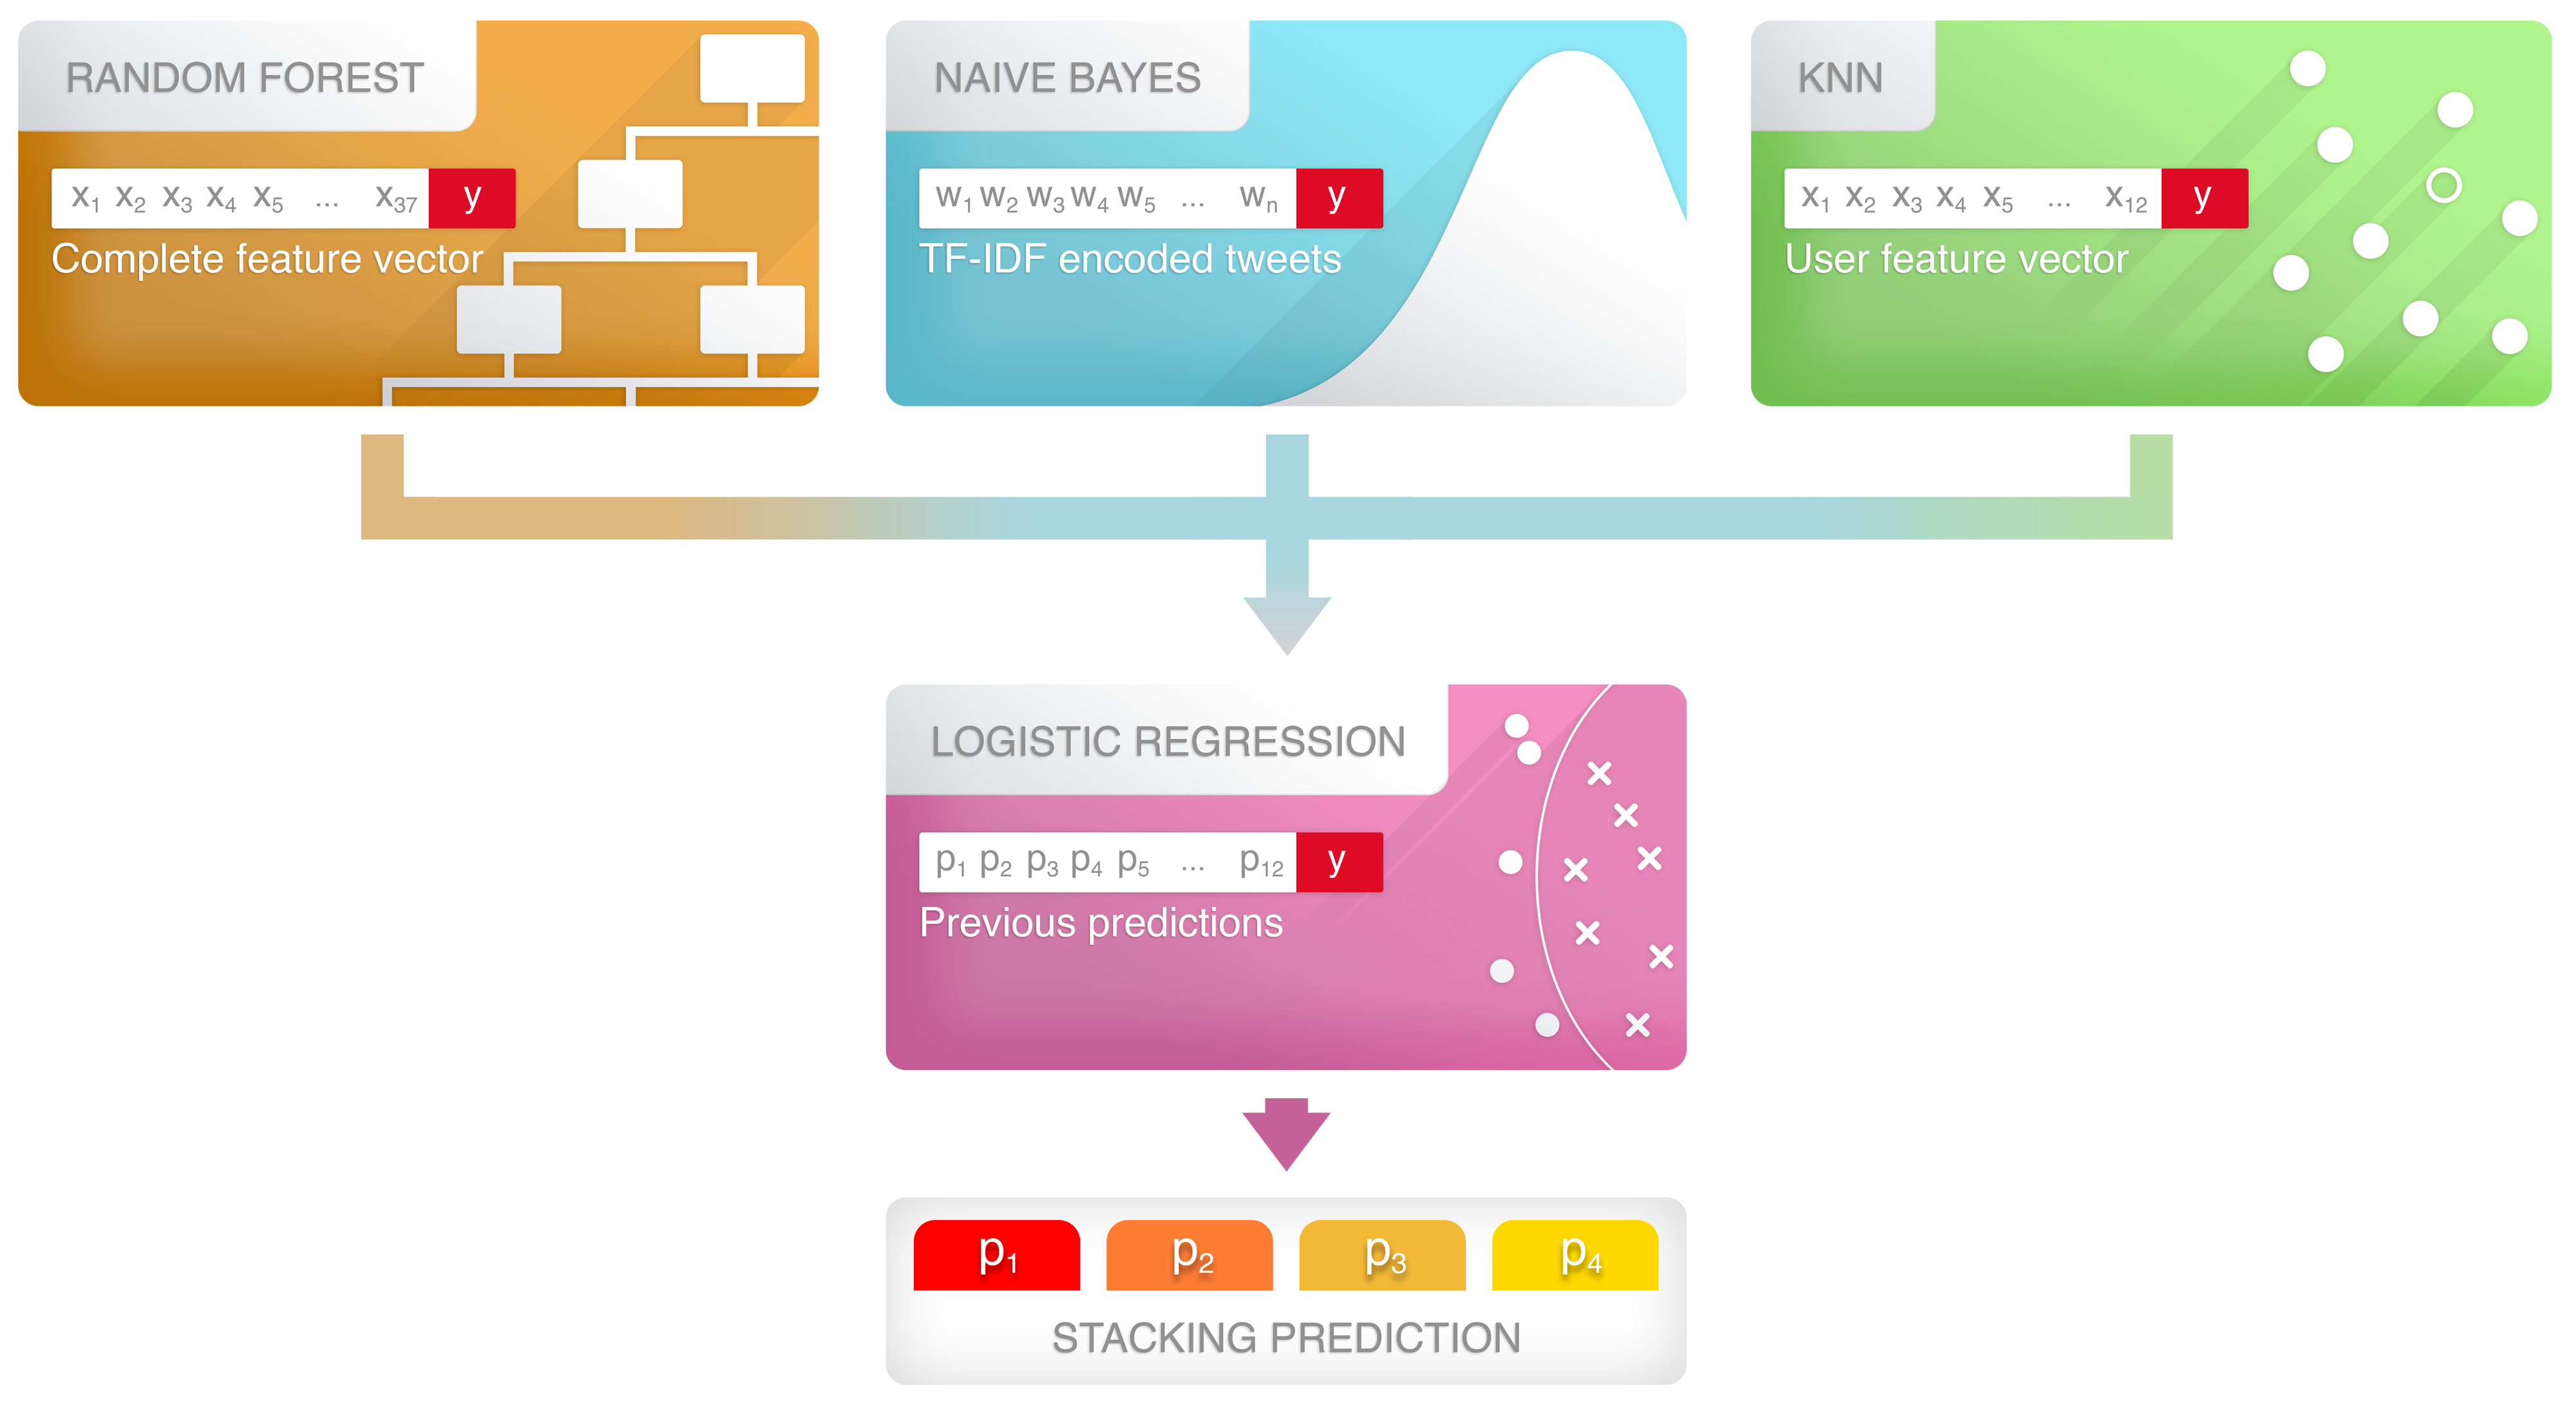
\includegraphics[width=\columnwidth]{chapter5/figure/stacking.png}
	\caption{Multi-class ensemble schema}
	\label{fig:stacking_schema}
\end{figure}
In the following subsections there are the detailed explanations of the three classifier announced before.

\subsection{All-features-based Random Forest classifier}
\subsubsection{Dataset}
During this phase, we used the previously described dataset \ref{sec:dataset} with its four different labels.
The algorithm was fed with 21,445 samples and 37 features. the amount of records were light enough to consider K-fold crossvalidation, without slow the validation down too much.
\subsubsection{Model}
We found ourselves in the situation in which we had some brand new features and we didn't know how useful they were. Obviously, we could appeal to heat-maps or other tools, to highlight the correlations among variables and targets.
However, the model we wanted to develop was the Random Forest, which proved to perform well with F1 score. Since this kind of model exploits its criteria to employ the features, we needed to prove them with a direct approach.

\subsubsection{Features selection}
A useful advantage of the Random Forest algorithm is the ability to provide a feature ranking, according to its splitting criterion.
We retrieved this standing, in order to see if we would have found some of the ones coming out from feature engineering at the top positions.
The algorithm ranking ranked the features this way: 1. \textit{favourites\_count} (0.179), 2. \textit{nsfw\_profile} (0.068), 3. \textit{freq} (0.061), 4. \textit{tweet\_intradistance} (0.060), 5. \textit{news\_spreaders\_words\_score} (0.058), 6. \textit{statuses\_count} (0.053), 7. \textit{avg\_len} (0.051), 8. \textit{followers\_count} (0.051), 9. \textit{NSFW\_words\_score} (0.043), 10. \textit{ret\_perc} (0.041), 11. \textit{min\_len} (0.038), 12. \textit{spam\_bots\_words\_score} (0.035), ...  37. \textit{min\_fav} (0.0001).

\begin{figure}[htp!]
	\centering
	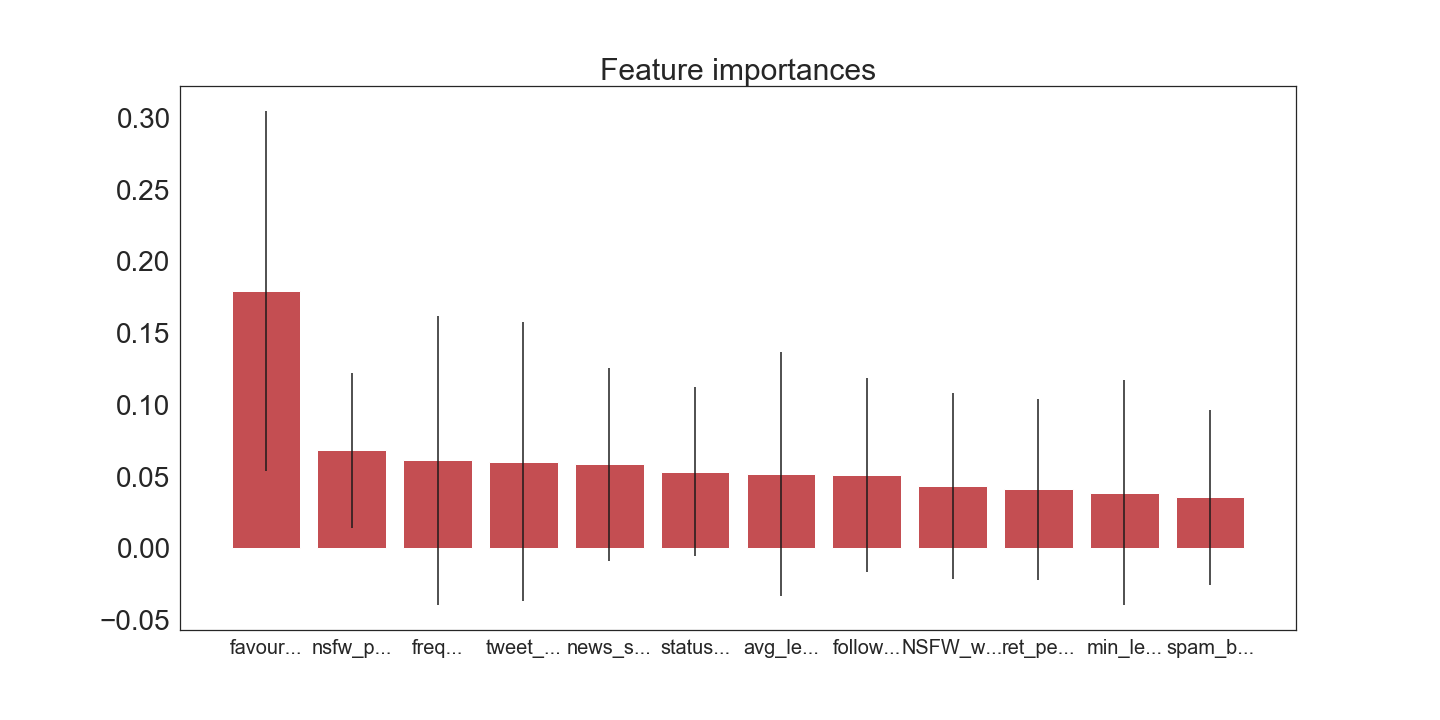
\includegraphics[width=\columnwidth]{chapter5/figure/top_12_features_importances.png}
	\caption{Random Forest top-12 feature ranking}
	\label{fig:feature_rank}
\end{figure}

As Figure \ref{fig:feature_rank} shows, we could find some of our crafted features inside this list: lots of tweets descriptive features (\textit{avg\_len, freq, ret\_perc}, etc...), as well as the \textit{tweet\_intradistance} attribute and three of the four extrinsic features, like \textit{news\_spreaders\_words\_score}, \textit{NSFW\_words\_score} and the \textit{spam\_bots\_words\_score}.
This picture confirmed us that the idea behind those features was useful.

Since those attributes were thought to belong to different clusters, we decided to try several combinations of those feature clusters, validating the model on them with a crossvalidation. The purpose of this stage was to see if some groups of features were enough to describe the real problem, or if some group would shown up as irrelevant.
To face this evaluation, we performed a light-weighted Grid Search, which is a method that takes desired ranges of hyperparameters and tries all the possible permutations of them, looking for the best combination, in terms of a certain metric.

We are talking about a light-weight version of this tool, because we just went through different numbers of tree estimators in the forest. The different feature groups are not considered as hyperparameters and are not handled by the Scikit-learn implementation of the Grid Search.
We had to manage the different training by our own, looking how the test score would have changed along with the increasing number of estimators and the different set of features.

Grid Search uses crossvalidation to find the better estimators for the models, and this approach was right for our situation.
Due to the multi-class nature and some imbalances with the labels, we decided to follow the F1 score metric to asses the value of our model.

The features were organized in clusters, as described in Chapter \ref{capitolo4}.
We had the user features, the descriptive features, the intrinsic features, the extrinsic and the image features. Then we tried the model with the entire set of 38 attributes.
As shown in Figure \ref{fig:feature_clusters}, the best configuration seems to involve the whole set of features, as it reaches these scores, with 100 estimators: \textit{Precision} = 0.978, \textit{Recall} = 0.976, \textbf{\textit{F1}}= 0.977.

\begin{figure}[htp!]
	\centering
	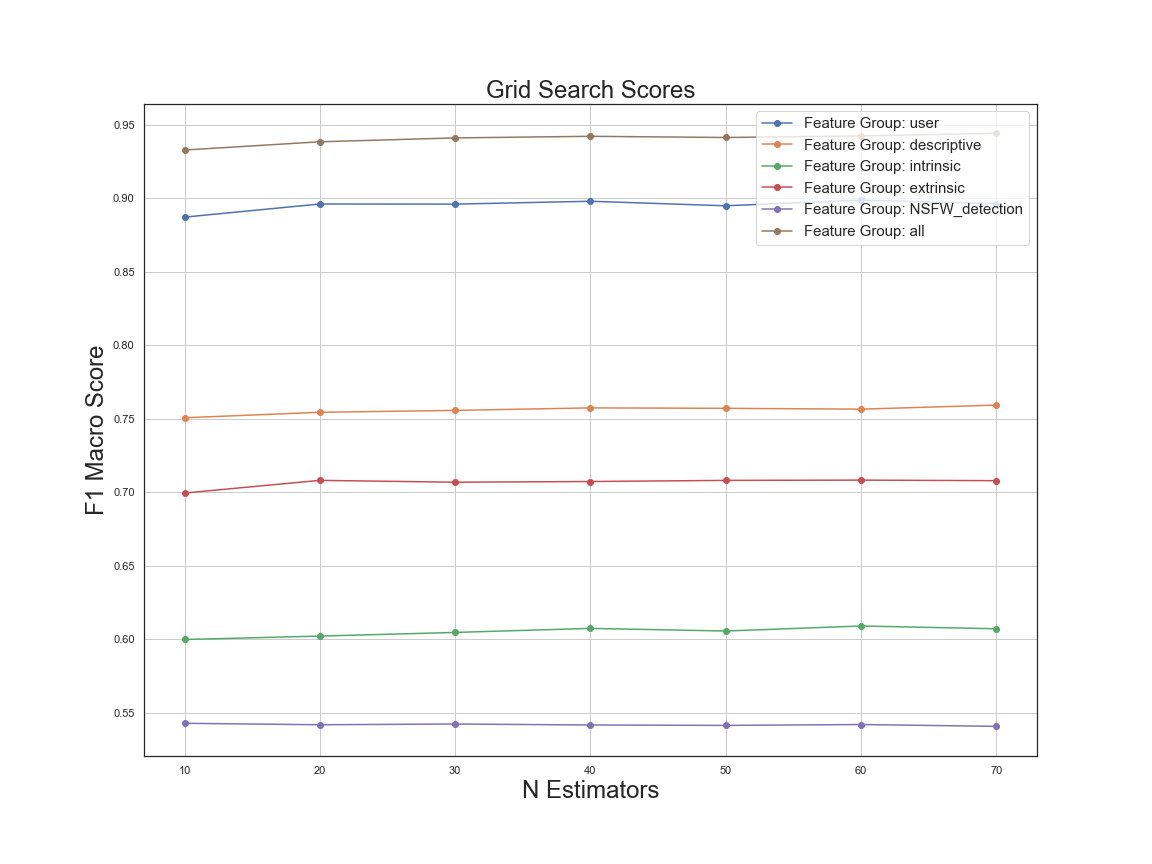
\includegraphics[width=\columnwidth]{chapter5/figure/feature_cluster_f1.png}
	\caption{Performance over different feature clusters}
	\label{fig:feature_clusters}
\end{figure}

The model has been tested with the default value for the maximum depth in the trees, which is set to 'None'. It means that the trees are expanded until every leaf is pure, or all leaves contain one sample.

In order to try all the alternatives, we setted a test involving the performance of the model, when it was working on an increasing number of features.
We had the ranking provided by the forest itself, so we started by testing only the most important attribute, adding one feature at time, until the least important was included.
We were looking for some changing in the scores, that would have pointed to a lighter model, with the exclusion of some features.
Figures \ref{fig:feat_prec}, \ref{fig:feat_rec}, \ref{fig:feat_f1} show the trends of the Precision, the Recall and the F1, respectively, along with the number of features tested.
 \begin{figure}[htp!]
 	\centering
 	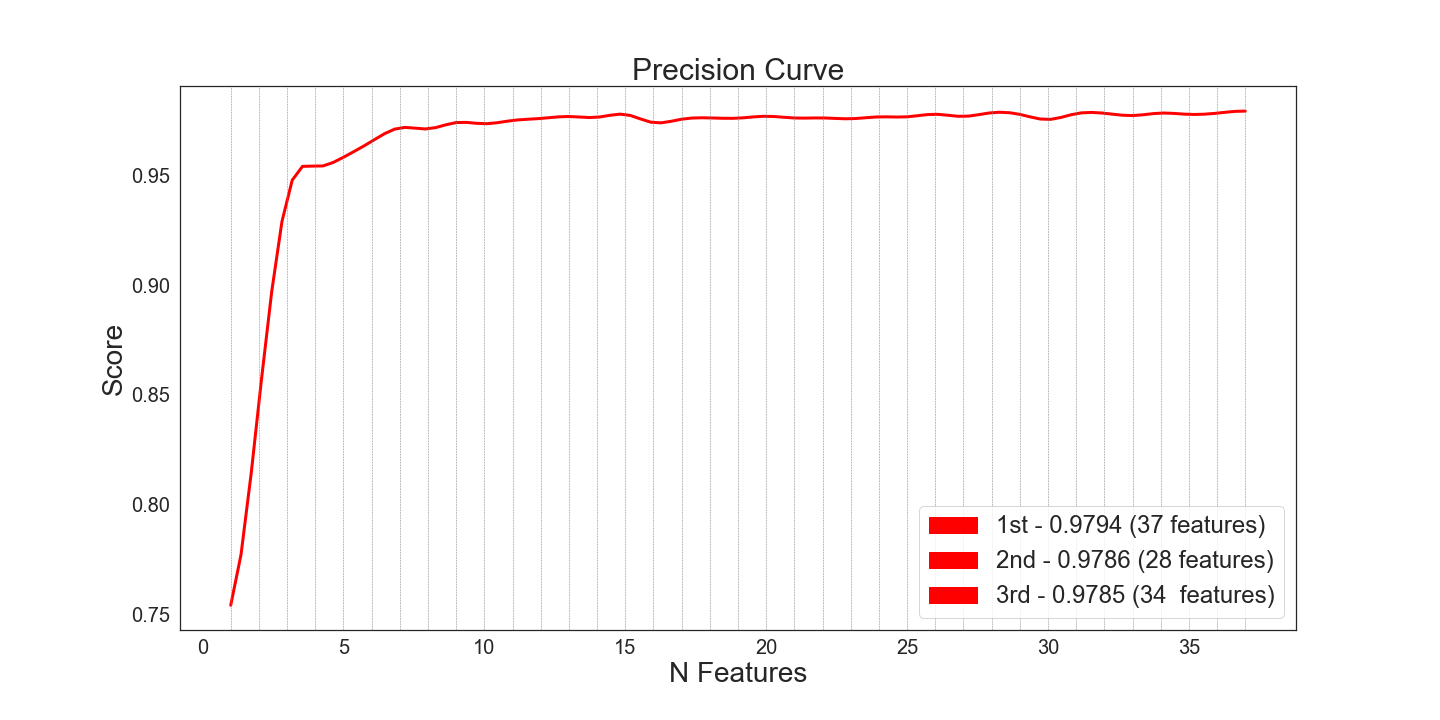
\includegraphics[width=\columnwidth]{chapter5/figure/precision_along_features.png}
 	\caption{Precision trend along with number of features tested}
 	\label{fig:feat_prec}
 \end{figure}
\begin{figure}[htp!]
	\centering
	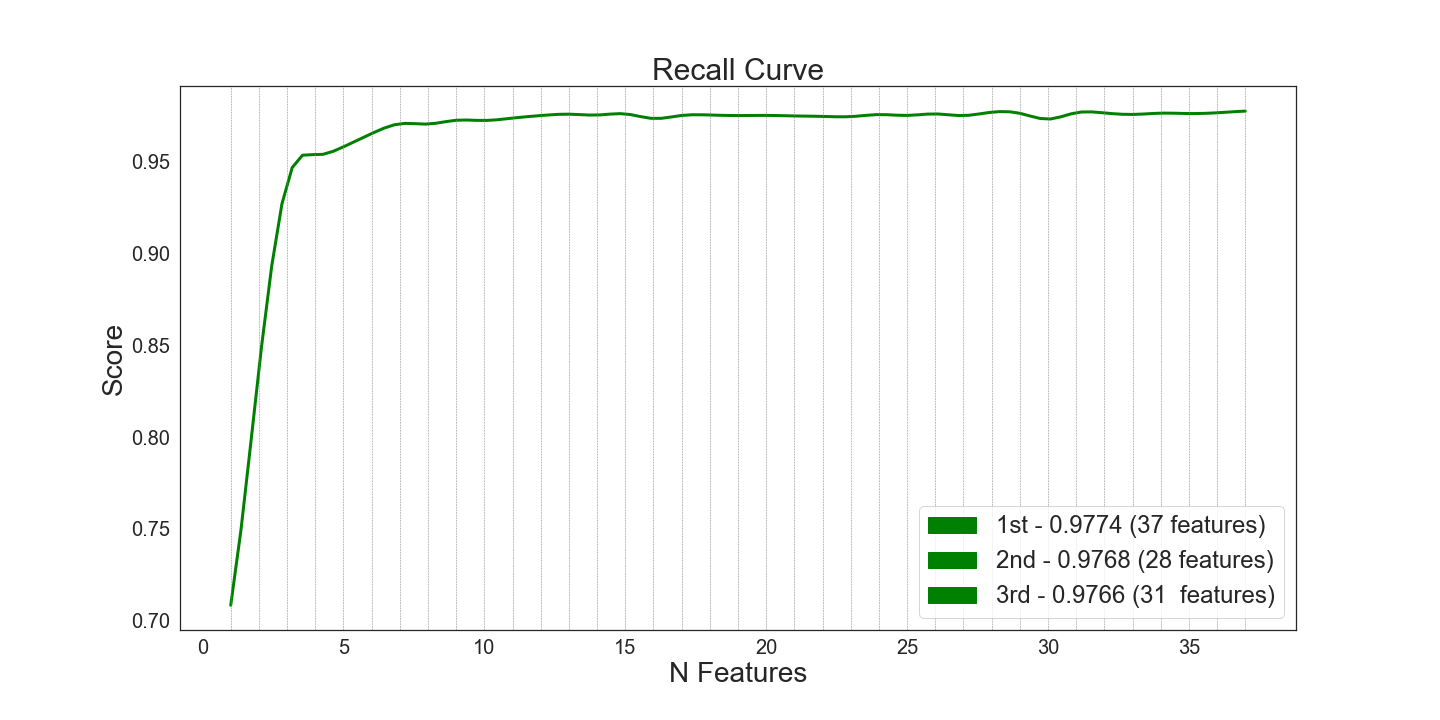
\includegraphics[width=\columnwidth]{chapter5/figure/recall_along_features.png}
	\caption{Recall trend along with number of features tested}
	\label{fig:feat_rec}
\end{figure}
\begin{figure}[htp!]
	\centering
	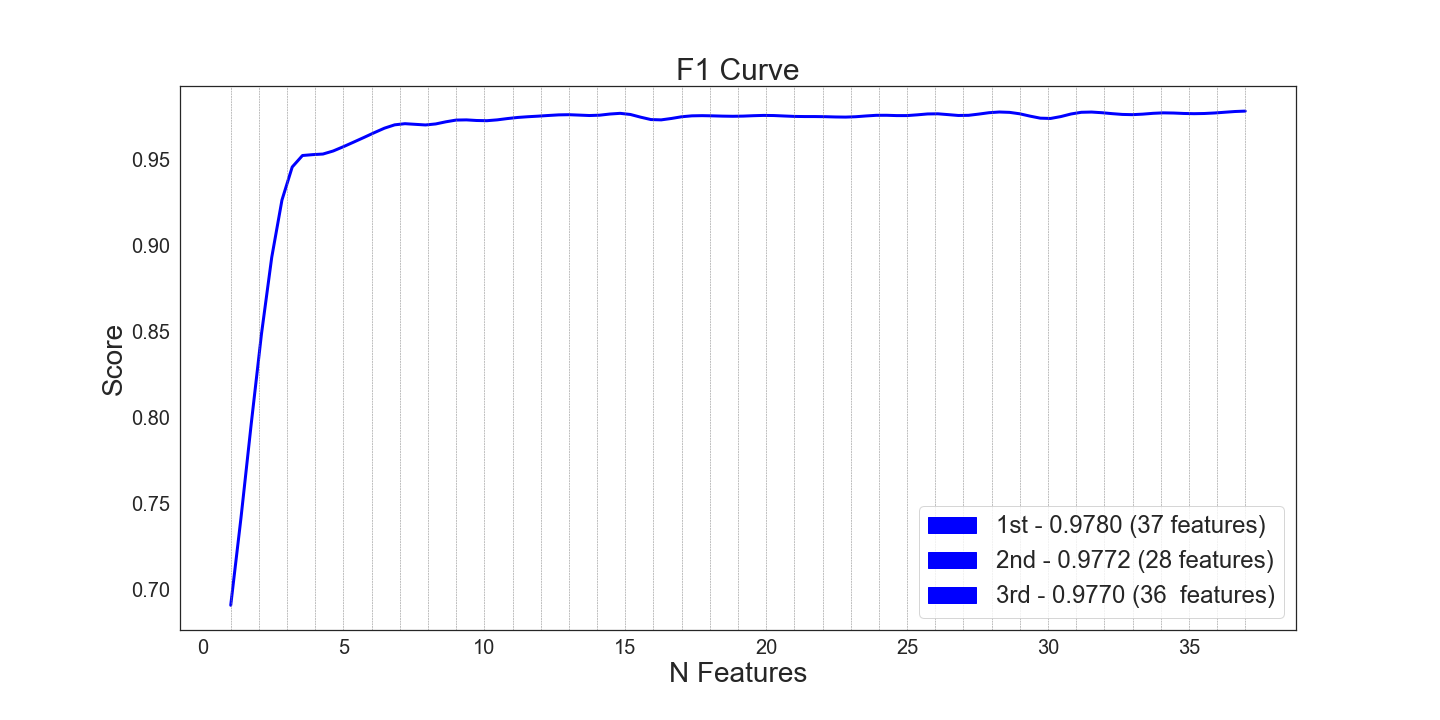
\includegraphics[width=\columnwidth]{chapter5/figure/f1_along_features.png}
	\caption{F1 trend along with number of features tested}
	\label{fig:feat_f1}
\end{figure}

As all the Figures show, the best solution possible, looking at both the three metrics, is the one involving all the 37 components of the feature vector.
There was the possibility to choose the second result, which wanted only the first 28 features, in terms of importance for the Random Forest. However, we weren't struggling with heavy models or long prediction times and the Random Forest algorithm handles the overfitting problem properly, even with complex models.
Thus, we moved on with the entire feature vector as support for the classification goal.

We then continued with a proper Grid Search over the whole number of features.
\subsubsection{Hyperparameters Tuning}
The algorithms rely on parameters in order to fit a problem.
Once the number of featured was picked, as well as the model, we needed to consider the possible hyperparameter ranges. 
The Grid Search method from Scikit-learn helped us, once again, during this exploration.
Since we were testing a Random Forest, we wanted to play with the number of estimators (tree) to include in the pool, as well as the maximum depth of each tree and the splitting criterion.

\begin{figure}[htp!]
	\centering
	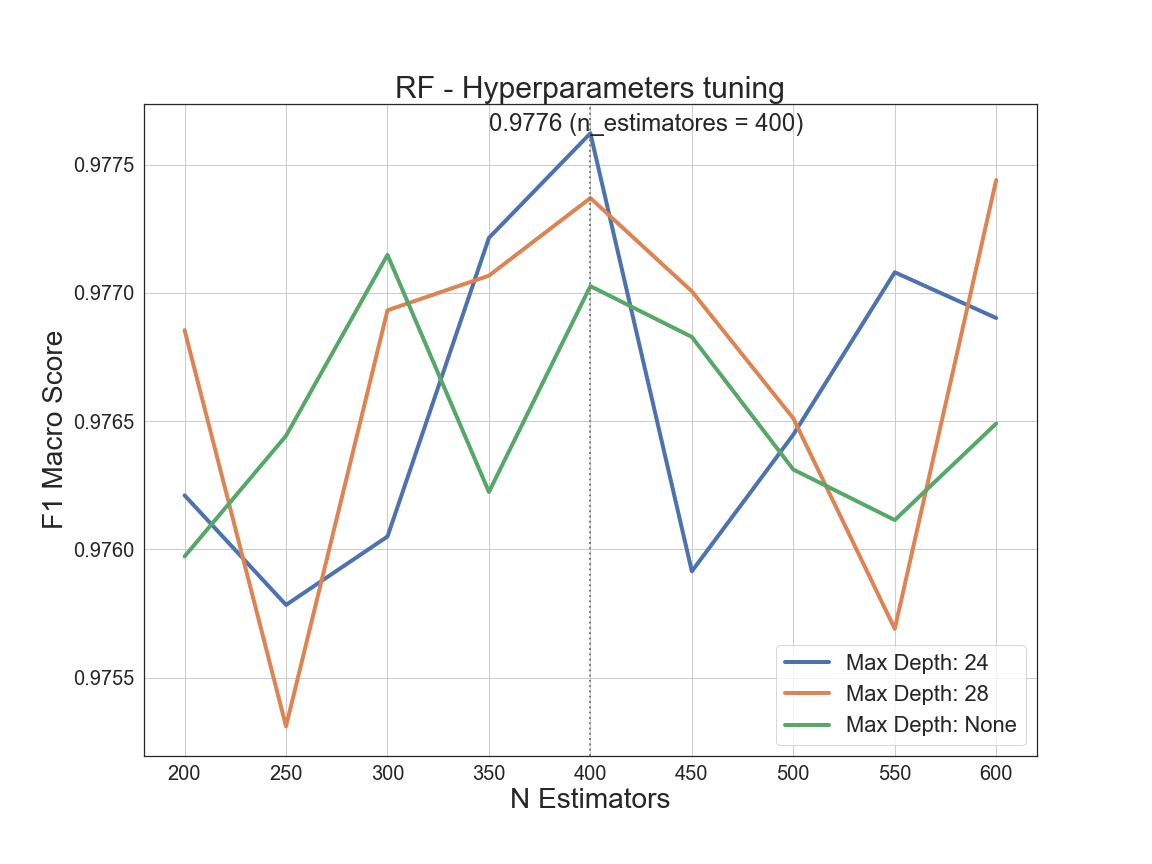
\includegraphics[width=\columnwidth]{chapter5/figure/multiclass_rf_tuning_gini.png}
	\caption{F1 scores with ``Gini`` criterion - close-up view}
	\label{fig:rf_tuning_gini}
\end{figure}
\begin{figure}[htp!]
	\centering
	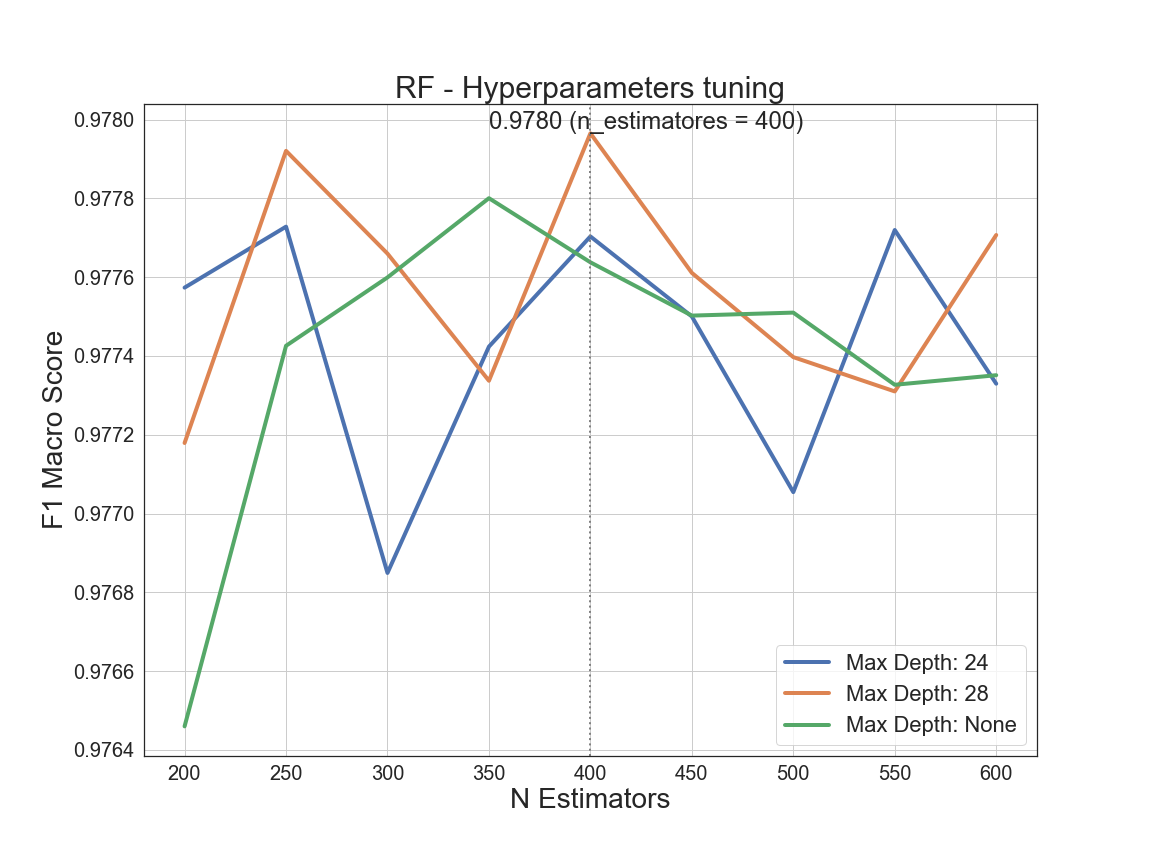
\includegraphics[width=\columnwidth]{chapter5/figure/multiclass_rf_tuning.png}
	\caption{F1 scores with ``Entropy`` criterion - close-up view}
	\label{fig:rf_tuning_entropy}
\end{figure}

The Figures \ref{fig:rf_tuning_gini}, \ref{fig:rf_tuning_entropy} show how the average F1 score, measured on 10-fold crossvalidation, changes with the increasing of the number of estimators in the forest.
The different coloured lines represent the \textit{max\_depth} hyperparameter.
The first Figure (\ref{fig:rf_tuning_gini}) shows the Grid Search results, with the \textit{gini} splitting criterion.
The second one (\ref{fig:rf_tuning_entropy}) represent the situation having \textit{entropy} as a splitting choice.
We combined nine numbers of estimators (200, 250, 300, 350, 400, 450, 500, 550, 600), together with three different maximum depths for the trees (26, 28, None) and the two above-mentioned splitting criteria.

We could observe a peak, for both criteria, in correspondence with 400 estimators.
Although the Gini-based forest's score didn't seem a bad point, we went with the Information Gain splitting criterion, which si also the same we used to rank the features of our data.

The final configuration involves 400 trees, the Information Gain criterion and the maximum reachable depth (for each of the 400 estimators) equal to 28 levels, yielding the following scores in 10-fold-crossvalidation:
\begin{itemize}
	\item[\PencilRight] \textit{Precision}: \textbf{0.979}
	\item[\PencilRight] \textit{Recall}: \textbf{0.977}
	\item[\PencilRight] \textit{F1 score}: \textbf{0.978}
\end{itemize}

Figure (\ref{fig:tree}) shows an example of one of the estimators of the final model, plotted with Matplotlib library for Python. It has been represented with the first two levels of depth, for visualizations reasons.

\begin{figure}[htp!]
	\centering
	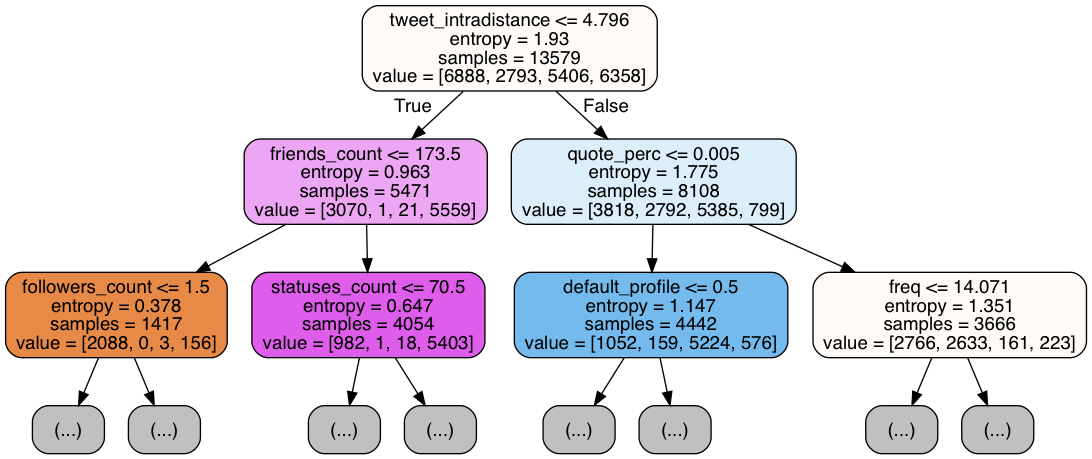
\includegraphics[width=\columnwidth]{chapter5/figure/tree.png}
	\caption{Tree estimator of the Random Forest model}
	\label{fig:tree}
\end{figure}

As the picture shows, this tree used the \textit{tweet\_intradistance} feature as root, in order to perform its first split on that attribute.

The first algorithm of the multi-class ensemble was completed and ready to be combined with the following models.

\subsection{User-based KNN classifier}
The Random Forest model represents somehow the core of the ensemble, as it was trained on the entire feature vector, with all the data we had for the purpose. A massive attention for parameters and features were given for that classifier. 
However, we wanted to put it into an ensemble, not to improve its already strong stability over outliers, but to support it with different perspectives.

We noticed, as shown in the previous Figure \ref{fig:feature_clusters}, that the user features were a good group to build a classifier on. Thus, we started thinking how to implement such support, and we basically looked at our baselines.

The model that had the best performance, not considering the Random Forest, was the K-Nearest Neighbors algorithm.

We didn't want this model to work the entire feature vector, because we knew that it would had been overlooked by the Random Forest. Instead, we wanted it to concentrate on the features that describe the users, without the information driven by their tweets. Therefore, we relied on the user features, with the extension of the image feature that assesses the NSFW score to the profile picture. This extension wa due to the fact that such feature doesn't need the user's tweets to be computed; it can be seen as one of the user features as the others of that group.

We hoped that treating the data before, or during, the training phase, would had brought to a good sustain for the first multi-class model, where needed.

\subsubsection{Dataset}
The dataset is composed of the same number (21,445) of samples of the first multitarget Random Forest, but preserving only the twelve features belonging to the user group, plus the NSFW\_profile attribute coming from the image features group.

\small
\begin{center}
	\begin{tabular}{ll}
		\\Feature vector\\
		\hline\hline
		default\_profile, favourites\_count, followers\_count\\
		friends\_count, listed\_count, screen\_name\_len\\
		statuses\_count, url, description\_len, NSFW\_profile\\
		name\_len, profile\_use\_background\_image, age\\\hline\\
	\end{tabular}
\end{center}
\normalsize

\subsubsection{Model}

This model is quite simple and doesn't require much effort in interpolating several hyperparameters. But this doesn't mean that it is a closed box algorithm. It can be improved by paying attentions to some details. In particular there had been done three considerations, and they were regarding

\begin{itemize}
	\item[\PencilRight]\textbf{Hyperparameters}\\
	The main hyperparameters that can be combined together are the number \textit{k} of neighbours ti consider, when performing a prediction, and the distance metric used by the calculations of the distances.
	The Scikit-learn implementation of the algorithm uses the \textit{Minkowski} metric, which describes the \textbf{L}\textsubscript{p} norm: 
	\[ \mathit{L_{p}} = (\sum\limits_{i = 1}^{n}|x_{i} - y_{i}|^{p})^{1/p} \]
	This metric is a generalization of the \textbf{L}\textsubscript{2} norm, also known as the Euclidean distance.
	The library we used allowed us to tune the \textit{p} hyperparameter, which indicates the metric used: \textit{p} = 1 means L\textsubscript{1} norm, the Manhattan Distance, when \textit{p} = 2 stands for the Euclidean.
	Higher values of \textit{p} are available, with other metric involved.
	
	We tried several values for both \textit{p} and \textit{k}, obtaining different results.
	However, the overall decision had to take in consideration also other two factors, the features weighting and the kernel function.
	
	\item[\PencilRight]\textbf{Features Weighting}\\
	The KNN algorithm aims to map the samples into a space and then it looks for the distances among them. In order to have best mapped space, it is reasonable to perform a weighting over the data. With this approach, the mapping would change and some points could result both as closer or more distant from each others.
	
	We performed some tests on four configurations. The first one didn't involve a weighting vector, while the second one was a standard normalization of the features.
	This last option provided weak results, with the same configurations of parameters, and thus were discarded from further analysis.

	The third option, which was the most interesting, was built by computing the Information Gain for each feature, using the inner ability of the Random Forest classifier, and then by applying the weights on the attributes, basing the coefficients on the scores provided by the ranking.
	This method emerged as the most effective, in the overall score.
	
	The last one was implemented as a Gaussian Kernel, which exploits the above-explained Radial Basis Function \ref{rbf}.
	This attempt fell shorter then the standard normalization, and it could be imputable to an overestimation of the ability to approximate the probability density of our data.
	It seemed that the Gaussian-based weighting wasn't a good fit for the problem.
\end{itemize}

We ran a Grid Search session over an increasing number of neighbours and the first four coefficients of the Minkowski distance.
All the combinations were tested with both the non-weighted data and the Entropy-based weighted data.
The results obtained are highlighted in Figure \ref{fig:knn_tuning}

\begin{figure}
	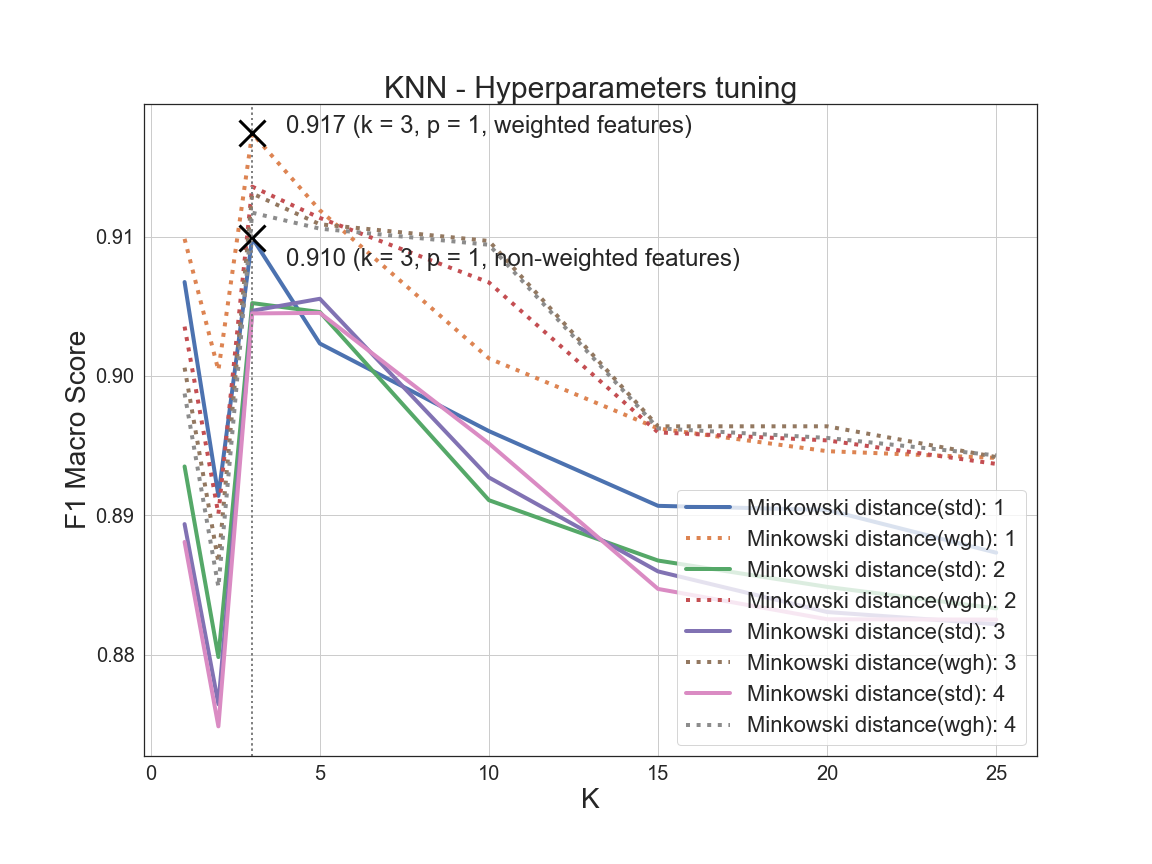
\includegraphics[width=\columnwidth]{chapter5/figure/knn_tuning.png}
	\caption{Hyperparameters p, k tuning, with different weightings}
	\label{fig:knn_tuning}
\end{figure}
The different colours represent the Minkowski distances tested, as well as the different line styles, dotted and continue, represent the weighted and the non-weighted solutions, respectively.

As visible in the picture, the best score, in the usual 10-fold crossvalidation, has been obtained with 5 neighbours, the Manhattan distance, and the weighted solution, which is averagely better than the other one.

The final model has been created with the following call: \textit{KNeighborsClassifier(p=1, n\_neighbors=5)} and it has been fitted with the weighted data, obtaining the following scores in 10-fold-crossvalidation:

\begin{itemize}
	\item[\PencilRight] \textit{Precision}: \textbf{0.924}
	\item[\PencilRight] \textit{Recall}: \textbf{0.917}
	\item[\PencilRight] \textit{F1 score}: \textbf{0.918}
\end{itemize}


\subsection{Text-based Naive Bayes classifier}
In chapter \ref{capitolo4} we created some useful features that helped the above-mentioned classifiers . Anyway we didn't consider enough the tweet texts. A first idea consisted in add a feature that describe the context of the tweets. This task was easily viable using \textit{Google Cloud Natural Language}. Unfortunately, this service only provides a few free calls, and we would not be able to tag all the tweets in our dataset. Moreover, the Context Classification is very specific, and we would have risked to have a too large domain of values. We tried to classify some tweets and we noticed that it was not possible with many of them, since they were just exclamations or contextless sentences. We therefore decided to train a proprietary text classifier. This allowed us to classify texts according to our targets, and our final classifier would have been self-sufficient, without external services.
\subsubsection{Dataset}
Since we wanted to classify texts instead of users, we needed to create a specific dataset.
It had to contain a list of tweets and all the related target. We composed it by binding the target of each tweet to the label of its author. This produced some noise; often bots tweet something different from their goal, to seem more humans. We could accept this problem, since most of the tweets are aimed to a goal.
The shape of the dataset is the following:

\begin{center}
	\begin{tabular}{lr}
		category&\# tweets\\
		\hline\hline
		NSFW&196712\\
		news\_spreaders&280300\\
		spam&453719\\
		fake\_followers&41316\\
		genuine&261233\\
		\hline\\\\
	\end{tabular}
\end{center}

It seems unbalanced, anyway it is appropriate to keep all the data. Some spambot's tweets just contain links and they will be removed in the next steps. Differently, Fake-followers usually don't tweet, or they never tweeted.

\subsubsection{Model}
In order to classify texts, we decided to use a Naive Bayes approach. This algorithm consists in a probabilistic classifier based on the Bayes' theorem. ``Numerous researchers proved that it is effective enough to classify the text in many domains \cite{svm}. Naive Bayes models allow each attribute to contribute towards the final decision equally and independently from other attributes`` \cite{nb}.

Tweets can't be processed as they are. Since this model aims to classify texts basing on its words, we had to clean the dataset from all those parts of the text that are not real or useful words. For example articles, smiles, punctuation should not be taken into consideration. Moreover it is fundamental to reduce inflected words to their word stem. Finally, we need to clean all those noisy parts of the tweets, which is important to allow the final text classifier to consider only real words, in order to identify the context.

Tweets without this pre-processing step look like this:\\

\framebox[\textwidth][l]{\parbox{\textwidth}{\textit{'RT @SteveSchmidtSES: TRUMP disgraced the Presidency and the\\United States at the G-7 summit. From his slovenly appearance to his\\unprepared... https://t.co/KiT29FvJw5'}}}\\

In order to perform this tasks, we used a \textit{sklearn Pipeline}. It is a method that allows to build a custom predictive algorithm. In our case, it contains intermediate steps of data transformation and finally the machine learning algorithm. It works like a generic model, but it perform all the included transformations before processing a data, both in training and prediction steps.

We added to the pipeline the following operations:

\begin{itemize}
	\item[\PencilRight] \textbf{Remove retweet information:}\\
	Delete the texual pattern which indicates that the current status is a retweet. It consists in a "RT @original\_author:". 
	\item[\PencilRight] \textbf{Remove punctuation:}\\
	With regular expressions we removed everythink different from characters and numbers. In this step also smiles and other symbols are removed.
	\item[\PencilRight] \textbf{Remove stopwords:}\\
	stopwords are the most common words that are always used in a language and that can not help to classify a context. Some example of words belonging to this category are articles or prepositions.
	We removed them, by using a stopwords dictionary of \textit{NLTK} libraries.
	\item[\PencilRight] \textbf{Transform uppercase characters into lowercase:}\\
	Before tokenize words, we transformed every character into lowercase, in order to be sure that every word is considered only in one form.
	\item[\PencilRight] \textbf{Apply stemming:}\\
	This is the step where words are reduce to their word stem. Since the text classifier is based on the occurrences of words in the texts, we don't need a correct grammar in our tweets. Instead, words at their basic form are more useful for the target.
	In order to perform this transformation we used \textit{SnowballStemmer} from \textit{NLTK} libraries.
	\item[\PencilRight] \textbf{Apply TF-IDF encoding:}\\
	Finally we applied to each word a TF-IDF encoding. Since we had a huge amount of tweets, without this step we would have risked to give too much importance to the overused wordsand almost nothing importance to the others. Moreover, without using TF-IDF we had a worse performance.
	\item[\PencilRight] \textbf{MultinomialNB:}\\
	This is the final classification algorithm. Thanks to the pipeline it always receives cleaned data, performing a better training and predictions.
	We selected a Naive Bayes classifier for multinomial models since we are dealing with a multi-class problem.
\end{itemize}

\subsubsection{Holdout evaluation}
The final text classifier has the following performance:
\begin{itemize}
	\item[\PencilRight] \textit{F1 score:} \textbf{0.71} with TF-IDF
	\item[\PencilRight] \textit{F1 score:} \textbf{0.64} without TF-IDF
\end{itemize}

Since the other models classify users and not single tweets, we could not use a classifier for texts only.
In order to get a prediction on users, based only on their tweets, the final classification script compute the resulted probabilities for each tweet. Then, for each user, the final prediction consists in the mean of the predictions over his tweets.
% !TEX root = ../thesis.tex
\chapter{Bot classifiers}
\label{capitolo5}
\thispagestyle{empty}

In this chapter we will show the choices and stages behind the final model.
Starting from baseline models, we enhanced the chosen classifiers with handcrafted features coming from the last chapter.\\
We saw and studied the performance improvements with validation approaches, and this phase led us to our current solution.

The result involves three models:
\begin{itemize}
	\item[\PencilRight] a first Random Forest classifier that has been used to provide an early filter on the separation between genuine accounts and bots
	\item[\PencilRight] a second Random Forest that gives a classification among the four studied categories of bots only
	\item[\PencilRight] a Naive Bayes classifier, used over the same classes of the second Random Forest, but which reads and labels the users, according on their tweets only
	\item[\PencilRight] a K-Nearest Neighbours classifier, used over the four bot classes, based on the user features only
\end{itemize}
The algorithms were used together into a pipeline work-flow, whose first step is the detection of bots from humans, thanks to the first binary Random Forest.
Then, the percentage of membership in the bot category is further split into four sub-percentages, which represent the prediction over the inner bot categories.
This last partition is performed by a stacking ensemble, whose goal is to combine the predictions of the three multi-class models.


\section{Baselines}
The choices explained in this section were made at the same time of the ones listed in the Baseline section of the last chapter.

This is, basically, the same stage of the above-mentioned, but in a model-driven perspective.
The features involved are the ones described in section \ref{baseline}, but we started from that base, to try different classifiers over it.
We chose to evaluate the performances of raw classifiers, for both the binary and the multi-class problem.
Each type of classifiers has been tested with the respective dataset, but considering only the baseline features of those data.

Furthermore, no parameters tuning has been applied, in order to minimize the results of our baselines classifier, with their standard settings.
\subsection{Random Forest}
Random forest is an ensemble learning method used in classification tasks and prediction ones as well.

The algorithm builds several \textit{decision trees} and the resulting output is provided by the mode of the predictions coming from the estimators in the forest.

Each decision tree is trained on a subset of the original data, formed by sampling with replacements the whole training set. They share the same splitting criterion, in order to build subtrees, which is the entropy:\\
Every tree computes the Information Gain of each feature, which is the difference, in terms of entropy, between the information gained on the data \textit{D}, before splitting on the attribute \textit{X}, and the one gained after the split, which provides \textit{n} subsets of \textit{D}.
\[{ \mathit{InformationGain(X)} = \mathit{Information(D)} - \mathit{Information_{X}(D)}}\]
where
\[{ \mathit{Information(D)} = - p_{1}\log p_{1} - ... - p_{n} \log p_{n}}\]
and
\[{ \mathit{Information_{X}(D)} = \frac{|D_{1}|}{|D|}Information(D_{1}) + ... + \frac{|D_{n}|}{|D|}Information(D_{n}) }\]
The attribute providing the highest InformationGain, against the others at the same level of the tree, is chosen to perform a split.

The feature set considered by each tree is a random subset of the original pool.

Due to its ability to face overfitting and to the feature importance ranking that it can provide, this tool is often preferred over other models belonging to the same category.

The advantage of preventing overfitting usually comes with a slower prediction time, because it needs enough estimators for this task.
But, for our purpose, there were enough estimators to face the variance problem without affecting the generalization speed.
\subsection{Logistic Regression}
Logistic regression is a common statistical model, that uses a sigmoid function to map the output of a linear regression on a normalized score, giving the probability, for each sample, to belong to the positive class, given its features and a weighting vector:
\[{\displaystyle P(\hat{y}_{i} = +1 | \vec{x}_{i}, \vec{w})={\frac {1}{1+e^{-\vec{w}h(\vec{x}_{i})}}}}\]

Where $ \hat{y}_{i} $ is the predicted target, over the  \textit{$i_{th}$} sample, \textit{$ \vec{x}_{i} $} is the feature vector of that sample, \textit{$ \vec{w} $} represents the weighting vector that has to be learned and \textit{h} is the activation function of the linear regression.

Logistic Regression searches for the weighting vector that matches the highest likelihood and, in order to do that, it minimizes a cross-entropy
error function, provided by the negative log of the likelihood:
\[{ \mathbf{L}(\vec{w}) = -\ln \prod\limits_{i=1}^{n} P(\hat{y}_{i} = +1 | \vec{x}_{i}, \vec{w})}\]

In multi-classes tasks, there are two possible approaches to face the problem:
\begin{itemize}
	\item[\PencilRight] a more general \textit{softmax} function to replace the logistic sigmoid, which assigns the probability, for the  \textit{$i_{th}$} sample, to belong to the class \textit{C}:
	\[{\displaystyle P(\mathbf{C}_{i} | \vec{x}_{i}, \vec{w})={\frac {e^{-\vec{w}h(\vec{x}_{i})}}{\sum\limits_{j = 1}^{n}e^{-\vec{w}h(\vec{x}_{j})}}}}\]
	\item[\PencilRight] ``One-vs-Rest`` method, which for each class builds a model that predicts the target class against all the others.
\end{itemize}
We decided to stick with the default settings of the libraries involved, so OvR was the approach used for the baseline.

\subsection{K-Nearest Neighbors}
K-Nearest Neighbors is an instance-based model used for classification, regression and pattern recognition. It is considered as a lazy learning algorithm, because all the computation is deferred until the prediction phase.
When it performs a classification over a new point, it looks for the \textit{K} nearest samples in the training set, according to a chosen metric, and it assigns, to the unseen sample, the mode of the targets of the retrieved neighbors.

The choices to make are the ones regarding the number \textit{K} of neighbors to consider, the weights to assign to them and the metric to calculate the distance with.
We used the default settings for the metric (\textit{Euclidean distance}) and for the weighting technique (\textit{uniform}), but we chose to consider 10 neighbors, because the automatic setting was \textit{K} = 5, which is the number of our possible targets.
We chose a \textit{K} that is large enough to make the model not too sensible to outliers, and restricted enough to sharpen the classes boundaries.

We first normalized the training data and then we fitted the algorithm on them, in order to simplify the distance computations.

\subsection{Support Vector Machine}
Support Vector Machine is a smart way to do instance-based learning. It can be seen as a generalization of the weighted KNN algorithm, with an arbitrary and feasible \textit{kernel function}, instead of the more generic dot product.

It can be summarised with a support vector $ \mathbf{\vec{x}} $ (a subset of the training set), a weighting vector $ \mathbf{\vec{w}} $ for them and a \textbf{kernel} \textit{K(x, x')} (a similarity function).

In order to make it work properly, three choices must be made:
\begin{itemize}
	\item[\PencilRight] a proper kernel, which is often selected according to experience and domain knowledge of the problem. We wanted to make things simple in this stage, so we used the default kernel function, which is the Radial Basis Function:\label{rbf}
	\[ K(x, x') = exp(- \frac{||x-x'||^{2}}{2\sigma^{2}}) \]
	with $ \sigma $ as a free parameter
	\item[\PencilRight] the weights $ \vec{w} $, which are obtained by maximizing the margin that splits the records belonging to different classes. Each samples are mapped into a space, thanks to what is known as the \textit{kernel trick}. The ``trick`` helps a linear classifier to work on a non-linear problem, applying the kernel function in the prediction phase.\\This process highlights the boundary that separates the points belonging to different classes.
	SVM aims to draw the boundary for the classes, in order to maximize the ``margin`` formed between the closest points that have different targets
	\item[\PencilRight] the support vector $ \vec{x} $, which comes as a consequence of choosing weights
\end{itemize}
Since we were still facing a multitarget problem, the binary nature of SVM must had been adapted to our needs. We decided, once again, to stick with the default setting for non-binary classifications, in order to have only raw baselines to compare.

The multi-target classification is handled with ``One-vs-One`` approach.
It considers all possible pairwise binary classifiers and so it leads to $\frac{N(N-1)}{2}$ individual binary classifiers, where N is the number of the classes in the problem.

In comparison with "One-vs-Rest" approach, ``One-vs-One`` is less sensitive to an imbalanced dataset, but it's more computationally expensive then the the other, which only builds N binary classifiers.
Despite our choices over methods and parameters weren't accurate in this stage as they were in the other ones, we decided to stick with this setting for SVM, because otherwise it would have led us to an irrelevant algorithm, in comparison with the above-mentioned.

\subsection{Comparison and baseline selection}
Different tasks imply different evaluation metrics. Every classifier was validated and selected according to certain indices of goodness. In particular, we followed a triple of metrics that involves Precision, Recall and F1, for the multi-class problem and we aimed to maximize AUC score for the binary case.
\subsubsection{Multi-class metric}
The selected baseline models were tested with a holdout approach at first, then with a crossvalidation method.
We built a Confusion Matrix for each model, in order to bring out goodness indices for each class, such as \textit{True Positive} (TP), \textit{False Positive} (FP) and \textit{False Negative} (FN).
The evaluation metrics considered are \textit{Precision}, \textit{Recall} and \textit{F1 score} and they work on the mentioned indices.
\begin{itemize}
	\item[\PencilRight] $ Precision = \frac{TP}{TP+FP} $\\
	It measures the proportion of positive identifications, for a given target, that was actually correct.
	\item[\PencilRight] $ Recall = \frac{TP}{TP+FN} $\\
	It measures the proportion of actual positive classifications that was identified correctly.
	\item[\PencilRight] $ F1 score = \frac{2(Precision \times Recall )}{Precision+Recall} $\\
	It calculates the harmonic mean of the previous metrics.
\end{itemize}
Every metric is adapted to fit a multi-class problem. For each class, it has been computed this set of measures, and then they were averaged without weights (macro average), in order to not take label imbalance into account.

\subsubsection{Binary metric}
Since this classifier was built for a different purpose, with respect to the multi-class models, the \textit{Area Under the Curve} score (AUC) is the metric we followed, both for baselines and the final model evaluation.
Area Under the Curve represents the goodness of a classifier, in terms of the integral of the \textit{Receiver Operating Characteristic} (ROC curve), defined over the variation of a decision treshold.

The ROC curve lies in a bi-dimensional space, which has the \textit{True Positive Ratio} ($ TPR =  \frac{TP}{TP+FN}$) on the Y-axis, and the False Positive Ratio ($ FPR =  \frac{FP}{FP+TN}$ ) on the X-axis.
In general, a classifier should accomplish more than 0.5 in AUC score, because that threshold represents a random guesser, which has the 50\% of probabilities to detect the actual class.
The more the AUC score tends to 1, the better is the ability of the classifier to distinguish among classes.

The motivation behind the adding of this new metric is that we had a balanced binary dataset, and this metric is a good fit for this kind of problem. Moreover, Botometer claims to have accomplished an AUC of 0.95, on a 10-fold crossvalidation test.
We wanted to get close to that score, using our crafted features.


\subsection{Holdout evaluation}
The holdout evaluation is performed separating the samples in the dataset into training and test subsets. The splitting process is randomized and it requires a bigger portion of the original dataset to be inserted in the training data, comparing to the amount of samples that will form the test set. A common choice is to use a third of the data to evaluate the model.

\subsection{Multi-class}
In this case, we decided to use 75\% of the data for the training set and 25\% for the test set. This choice is a little bit different from the most common one, which builds the training set with 2/3 of the whole data, because we didn't dispose of a huge amount of records, so we preferred this ratio and then trying an other validation method for comparison.
Here we list the algorithms and their parameters, as they were written according to the Scikit-learn library for Python, their confusion matrix and their scores:
\begin{itemize}
	\item[\PencilRight] \textit{RandomForestClassifier(n\_estimators = 10, criterion = 'entropy')}\\
	Confusion matrix:
	
	{
		\centering
		\begin{tabular}{@{}cc|cccc@{}}
			\multicolumn{1}{c}{} &\multicolumn{1}{c}{} &\multicolumn{4}{c}{Predicted class} \\ 
			\multicolumn{1}{c}{} & 
			\multicolumn{1}{c|}{} & 
			\multicolumn{1}{c}{NSFW} & 
			\multicolumn{1}{c}{NS} &
			\multicolumn{1}{c}{SB} & 
			\multicolumn{1}{c}{FF} \\
			\cline{2-6}
			\multirow[c]{4}{*}{\rotatebox[origin=tr]{90}{Actual class}}
			& NSFW  & 1690 & 27 & 12 & 6\\
			& NS  & 27  & 785 & 30 &  0\\
			& SB  & 14  & 39 & 1280 & 5\\
			& FF  & 12 &  7 &  18 & 1215\\
			\cline{2-6}\\
		\end{tabular}\\
	}
	
	Precision: 0.957\\
	Recall: 0.958\\
	F1 score: 0.957

	\item[\PencilRight] \textit{LogisticRegression(fit\_intercept=True, max\_iter=100, penalty='l2')}\\
	Confusion matrix:
	
	{
		\centering
		\begin{tabular}{@{}cc|cccc@{}}
			\multicolumn{1}{c}{} &\multicolumn{1}{c}{} &\multicolumn{4}{c}{Predicted class} \\ 
			\multicolumn{1}{c}{} & 
			\multicolumn{1}{c|}{} & 
			\multicolumn{1}{c}{NSFW} & 
			\multicolumn{1}{c}{NS} &
			\multicolumn{1}{c}{SB} & 
			\multicolumn{1}{c}{FF} \\
			\cline{2-6}
			\multirow[c]{4}{*}{\rotatebox[origin=tr]{90}{Actual class}}
			& NSFW  & 1274 & 213 & 197 & 51\\
			& NS  & 24 & 740 & 75 & 3\\
			& SB  & 29 & 87 & 1144 & 78\\
			& FF  & 204 &  49 &  46 & 953\\
			\cline{2-6}\\
		\end{tabular}\\
	}
	
	Precision: 0.793\\
	Recall: 0.807\\
	F1 score: 0.794
	
	\item[\PencilRight] \textit{KNeighborsClassifier(n\_neighbors=10)}\\
	Confusion matrix:
	
	{
		\centering
		\begin{tabular}{@{}cc|cccc@{}}
			\multicolumn{1}{c}{} &\multicolumn{1}{c}{} &\multicolumn{4}{c}{Predicted class} \\ 
			\multicolumn{1}{c}{} & 
			\multicolumn{1}{c|}{} & 
			\multicolumn{1}{c}{NSFW} & 
			\multicolumn{1}{c}{NS} &
			\multicolumn{1}{c}{SB} & 
			\multicolumn{1}{c}{FF} \\
			\cline{2-6}
			\multirow[c]{4}{*}{\rotatebox[origin=tr]{90}{Actual class}}
			& NSFW  & 1578 & 36 & 60 & 61\\
			& NS  & 81 & 685 & 63 & 13\\
			& SB  & 81 & 32 & 1187 & 38\\
			& FF  & 104 & 6 & 55 & 1087\\
			\cline{2-6}\\
		\end{tabular}\\
	}
	
	Precision: 0.883\\
	Recall: 0.869\\
	F1 score: 0.875
	
	\item[\PencilRight] \textit{SVC(kernel='rbf', decision\_function\_shape='ovo')}\\
	Confusion matrix:
	
	{
		\centering
		\begin{tabular}{@{}cc|ccc@{}}
			\multicolumn{1}{c}{} &\multicolumn{1}{c}{} &\multicolumn{3}{c}{Predicted class} \\ 
			\multicolumn{1}{c}{} & 
			\multicolumn{1}{c|}{} & 
			\multicolumn{1}{c}{NSFW} & 
			\multicolumn{1}{c}{SB} & 
			\multicolumn{1}{c}{FF} \\
			\cline{2-5}
			\multirow[c]{3}{*}{\rotatebox[origin=tr]{90}{Actual class}}
			& NSFW  & 1735 & 0 & 0\\
			& NS  & 842 & 0 & 0\\
			& SB  & 1114 & 223 & 1\\
			& FF  & 483 & 0 & 769\\
			\cline{2-5}\\
		\end{tabular}\\
	}
	
	Precision: 0.603\\
	Recall: 0.445\\
	F1 score: 0.408
	
\end{itemize}

From these evaluations it is possible to see how the Random Forest algorithm outperforms Logistic Regression and Support Vector Machine. This difference colud be driven by the multi-class task. Logistic Regression and SVM need to be adapted to this purpose. Another factor that can discriminate the performances is the choices of the features and their magnitude. Random Forest doesn't require attribute normalization to top its scores, additionally, every feature has been ranked and tested with the inner feature ranking provided by the algorithm. It is possible that some of these attributes need further processing to better support the other models tested.


\subsubsection{Binary}
This evaluation was made with the common splitting ration between train and test set. Since we had 31,212 samples available, well balanced, we used two thirds (20,808) for the training set and the remaining (10,404) for the test set.
We wanted a first term of comparison, so, in the beginning, we evaluated the AUC metric with the holdout technique.
\begin{itemize}
	\item[\PencilRight] \textit{RandomForestClassifier(n\_estimators = 10, criterion = 'entropy')}\\
	Confusion matrix:
	
	{
		\centering
		\begin{tabular}{@{}cc|cc@{}}
			\multicolumn{1}{c}{} &\multicolumn{1}{c}{} &\multicolumn{2}{c}{Predicted class} \\ 
			\multicolumn{1}{c}{} & 
			\multicolumn{1}{c|}{} & 
			\multicolumn{1}{c}{BOT} & 
			\multicolumn{1}{c}{GEN}  \\
			\cline{2-4}
			\multirow[c]{2}{*}{Actual class}
			& BOT  & 4314 & 336\\
			& GEN  & 554 & 4160\\
			\cline{2-4}
			\multicolumn{2}{r|}{AUC} & 
			\multicolumn{2}{l}{0.905}\\
		\end{tabular}\\
	}

	\item[\PencilRight] \textit{LogisticRegression(fit\_intercept=True, max\_iter=100, penalty='l2')}\\
	Confusion matrix:
	
	{
		\centering
		\begin{tabular}{@{}cc|cc@{}}
			\multicolumn{1}{c}{} &\multicolumn{1}{c}{} &\multicolumn{2}{c}{Predicted class} \\ 
			\multicolumn{1}{c}{} & 
			\multicolumn{1}{c|}{} & 
			\multicolumn{1}{c}{BOT} & 
			\multicolumn{1}{c}{GEN}  \\
			\cline{2-4}
			\multirow[c]{2}{*}{Actual class}
			& BOT  & 3124 & 1526\\
			& GEN  & 558 & 4156\\
			\cline{2-4}
			\multicolumn{2}{r|}{AUC} & 
			\multicolumn{2}{l}{0.776}\\
		\end{tabular}\\
	}

	
	\item[\PencilRight] \textit{KNeighborsClassifier(n\_neighbors=10)}\\
	Confusion matrix:
	
	{
		\centering
		\begin{tabular}{@{}cc|cc@{}}
			\multicolumn{1}{c}{} &\multicolumn{1}{c}{} &\multicolumn{2}{c}{Predicted class} \\ 
			\multicolumn{1}{c}{} & 
			\multicolumn{1}{c|}{} & 
			\multicolumn{1}{c}{BOT} & 
			\multicolumn{1}{c}{GEN}  \\
			\cline{2-4}
			\multirow[c]{2}{*}{Actual class}
			& BOT  & 3698 &  952\\
			& GEN  & 1129 & 3585\\
			\cline{2-4}
			\multicolumn{2}{r|}{AUC} & 
			\multicolumn{2}{l}{0.777}\\
		\end{tabular}\\
	}

	
	\item[\PencilRight] \textit{SVC(kernel='rbf')}\\
	Confusion matrix:
	
	{
		\centering
		\begin{tabular}{@{}cc|cc@{}}
			\multicolumn{1}{c}{} &\multicolumn{1}{c}{} &\multicolumn{2}{c}{Predicted class} \\ 
			\multicolumn{1}{c}{} & 
			\multicolumn{1}{c|}{} & 
			\multicolumn{1}{c}{BOT} & 
			\multicolumn{1}{c}{GEN}  \\
			\cline{2-4}
			\multirow[c]{2}{*}{Actual class}
			& BOT  & 4625 & 25\\
			& GEN  & 4676 & 38\\
			\cline{2-4}
			\multicolumn{2}{r|}{AUC} & 
			\multicolumn{2}{l}{0.501}\\
		\end{tabular}\\
	}

\end{itemize}

Once again, Random Forest has the best scores, even in the binary problem. Although, e can see a worsening in the KNN performances in this test. It can be imputable to an ``unlucky`` holdout set or to the fixed parameters tested.

\subsection{Crossvalidation}
This approach is based on repeated holdouts. It is performed by splitting the whole data in \textit{K} non-overlapping folds, leading to \textit{K} different holdout evaluations. The results for each step are stored and the final evaluation is given by the mean of the \textit{K} evaluations. For each evaluation, one fold is used for testing, the other ones for training the models. A common practice is to set \textit{K = 10} and thus averaging 10 different evaluations.
This method is also known as \textit{K-fold crossvalidation}. We used a stratified approach, which takes care about keeping the labels balanced on each fold.

Due the need of performing ten steps, it is computationally more expensive then a simple holdout validation. In our case, it was feasible, in term of speed, because of the models complexity and the data amount. This situation held for both the binary and the mutliclass tasks.

The obtained scores are also more meaningful, with regards to holdout, because they are less sensitive to ``lucky`` or ``unlucky`` splits.

Here is the results for every baseline model:
\subsubsection{Multi-class}
\begin{itemize}
	\item[\PencilRight] \textit{RandomForestClassifier(n\_estimators = 10, criterion = 'entropy')}\\
	Mean precision: 0.947\\
	Mean recall: 0.945\\
	Mean f1 score: 0.943
	\item[\PencilRight]\textit{LogisticRegression(fit\_intercept=True, max\_iter=100, penalty='l2')}\\
	Mean precision: 0.827\\
	Mean recall: 0.815\\
	Mean f1 score: 0.815
	\item[\PencilRight]\textit{KNeighborsClassifier(n\_neighbors=10)}\\
	Mean precision: 0.878\\
	Mean recall: 0.858\\
	Mean f1 score: 0.862
	\item[\PencilRight]\textit{SVC(kernel='rbf', decision\_function\_shape='ovo')}\\
	Mean precision: 0.573\\
	Mean recall: 0.456\\
	Mean f1 score: 0.413
\end{itemize}

As the results show, the Random Forest algorithm is the one that achieves the best performances, even with default settings, on both holdout and 10-fold crossvalidation. We thus decided to consider it as the main tool to build our bot categories classifier. 
\subsubsection{Binary}
\begin{itemize}
	\item[\PencilRight] \textit{RandomForestClassifier(n\_estimators = 10, criterion = 'entropy')}\\
	Mean AUC: 0.916\\
	\item[\PencilRight]\textit{LogisticRegression(fit\_intercept=True, max\_iter=100, penalty='l2')}\\
	Mean AUC: 0.792\\
	\item[\PencilRight]\textit{KNeighborsClassifier(n\_neighbors=10)}\\
	Mean AUC: 0.835\\
	Mean precision: 0.779\\
	\item[\PencilRight]\textit{SVC(kernel='rbf')}\\
	Mean AUC: 0.583\\
\end{itemize}
Even in the binary cases, the Random Forest had the best performance, and it could be imputed to the similar features involved in both problems. Moreover, we could see that the Support Vector Machine emerged as a lightly improved random guesser.


\section{Binary Classifier}
Since our dataset was pretty balanced and we couldn't retrieve many more genuine accounts, we didn't want our instrument to treat this category of users just as one the other bot kinds. It was important to perform a previous filter that was able to give importance to the separation between bots and genuine accounts.

We were inspired by the work made with Botometer \cite{Botometer}, which involved a binary labelled dataset, with bot and genuine accounts.
The researchers built their features, grouped them in six main categories, then they ran a Random Forest algorithm per group.

We already had our feature engineering done, so we decided to test it on this new task.

In order to not to build a poorer version of our multi-class model, we didn't want to use a reduced copy of our dataset, stratifying it by stripping random bots from it. We needed a balanced dataset, with about the same amount of genuines and bots. So, we started from the same dataset used by the Botometer project, in order to have a baseline comparison.
\subsection{Dataset}
The dataset we used for this classification was composed of part of our collected records and of some entries from the Caverlee-2011 dataset, which contains 22,223 content polluters and 19,276 legitimate users, both collected through a social honeypot, as described in their paper \cite{Lee11sevenmonths}.

We used the APIs to retrieve the ids for both genuines and bots, from the Caverlee list. The process provided us 15,687 legitimate user ids, and 15,525 general bot ids (without inner classifications), for a total number of 31,212 samples.
The difference from the original number of entries is due to the age of the dataset. Since 2011, the year of the creation of the list, a lot of accounts have been deleted or suspended.

The feature vector we used is the same that came out from the feature engineering process, except for the specific characterizing features, that weren't considered, because crafted for the inner separation among bots. We excluded the \textit{NSFW\_avg}) image feature, as we noticed it didn't bring much performance boosting with the multi-class models.
The extrinsic features must had been adjusted with new dictionaries, so we had two features: (\textit{bots\_words\_score} and  \textit{genuine\_words\_score}.
Both the features have been computed as for the multi-class case, with up to 1000 non overlapping words in each dictionary.

\subsection{Model}
The model chosen for the purpose was the best performer of the tested baselines: the Random Forest binary classifier.
The algorithm has had its parameters tuned during the validation phase.
We decided to stick with 10-fold crossvalidation, as it was done for the baselines.

After several Grid Search runs, the last round computed had this hyperparameters to combine together:
\begin{itemize}
	\item[\PencilRight] \textit{n\_estimators} = [150, 200, 250, 300, 350, 400, 450, 500]
	\item[\PencilRight]\textit{max\_depth} = [None, 26, 28]
	\item[\PencilRight]\textit{criterion} = 'entropy'
\end{itemize}
\begin{figure}[htp!]
	\centering
	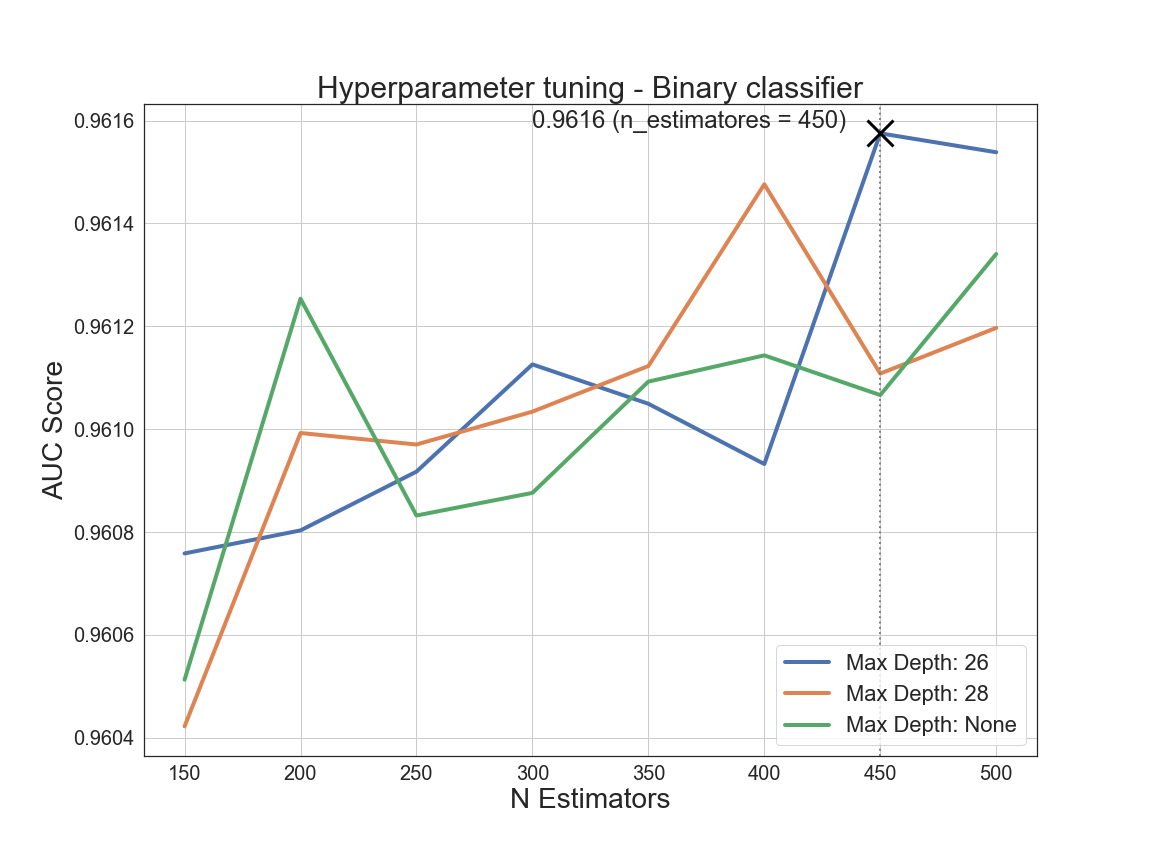
\includegraphics[width=\columnwidth]{chapter5/figure/bon_tuning.png}
	\caption{Grid search results}
	\label{fig:grid_search}
\end{figure}
\begin{figure}[htp!]
	\centering
	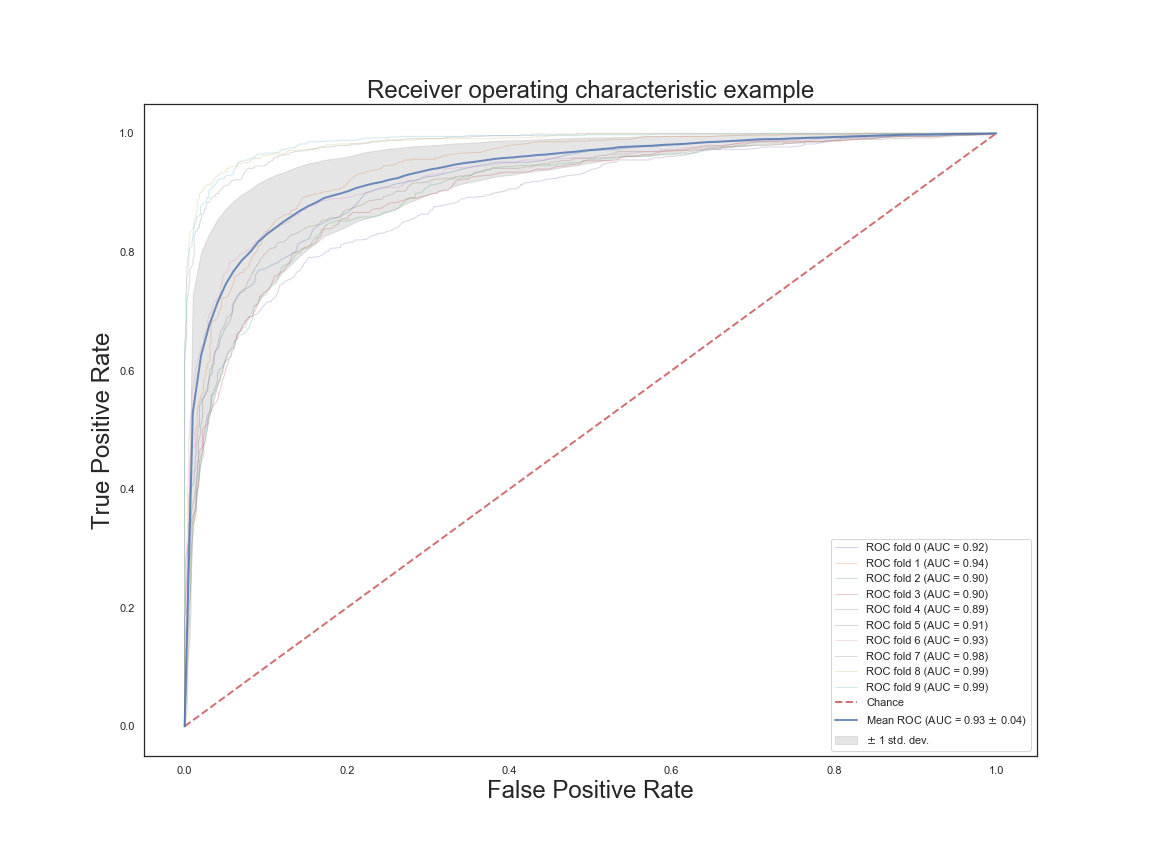
\includegraphics[width=\columnwidth]{chapter5/figure/auc.png}
	\caption{ROC curve}
	\label{fig:auc}
\end{figure}
As we can see in Figure \ref{fig:grid_search}, the AUC is increasing with the number of the estimators in the forest. We decided t stop at 450, which corresponds to the highest AUC score, since this phase was aimed to find a comparison term with Botometer, but it didn't represent the final model.
In their paper \cite{Varol}, the Botometer group claims to reach 0.95 in AUC score.

The AUC obtained with our arrangement is equal to 0.96, as shown in Figure \ref{fig:auc}, which is a positive accomplishment, considering that it will be used only as support for the identification of humans among bots, but we didn't crafted specific features as the ones involved in the Botometer project and we didn't have the same amount of data neither.

The model has then been fitted with the hole data, with this settings: \textit{ n\_estimators} = 450, \textit{max\_depth} = 26 and \textit{criterion} = 'entropy'.

\subsection{Validation}

We had an interesting amount of data that were not involved in this task, because of the comparison with the same Botometer's dataset. Since this unseen data had a further discrimination among bots, it was easy to sample some records randomly, replacing their multi-class targets with binary values.
We performed this job to validate the newborn model on unseen and fresher data.
We were interested in testing a model that were trained over ``old`` accounts, with consequent different attributes values and different behaviours on the platform, with younger accounts.

This validations would had given us a preview of the real performance of the model, once it would had been deployed on the internet. The account that a user would test with our application could be younger than the ones included in the Caverlee's list.

We sampled 6,000 accounts, divided in 3,000 genuine and 3,000 bot ids, randomly picked by our multi-class dataset.

The binary model were fitted with its data and it was ready to perform new predictions.

Looking at the most relevant features for the classifier, as shown in Figure \ref{fig:bon_importances}, we could find the \textbf{age} field at the top position.

\begin{figure}[htp!]
	\centering
	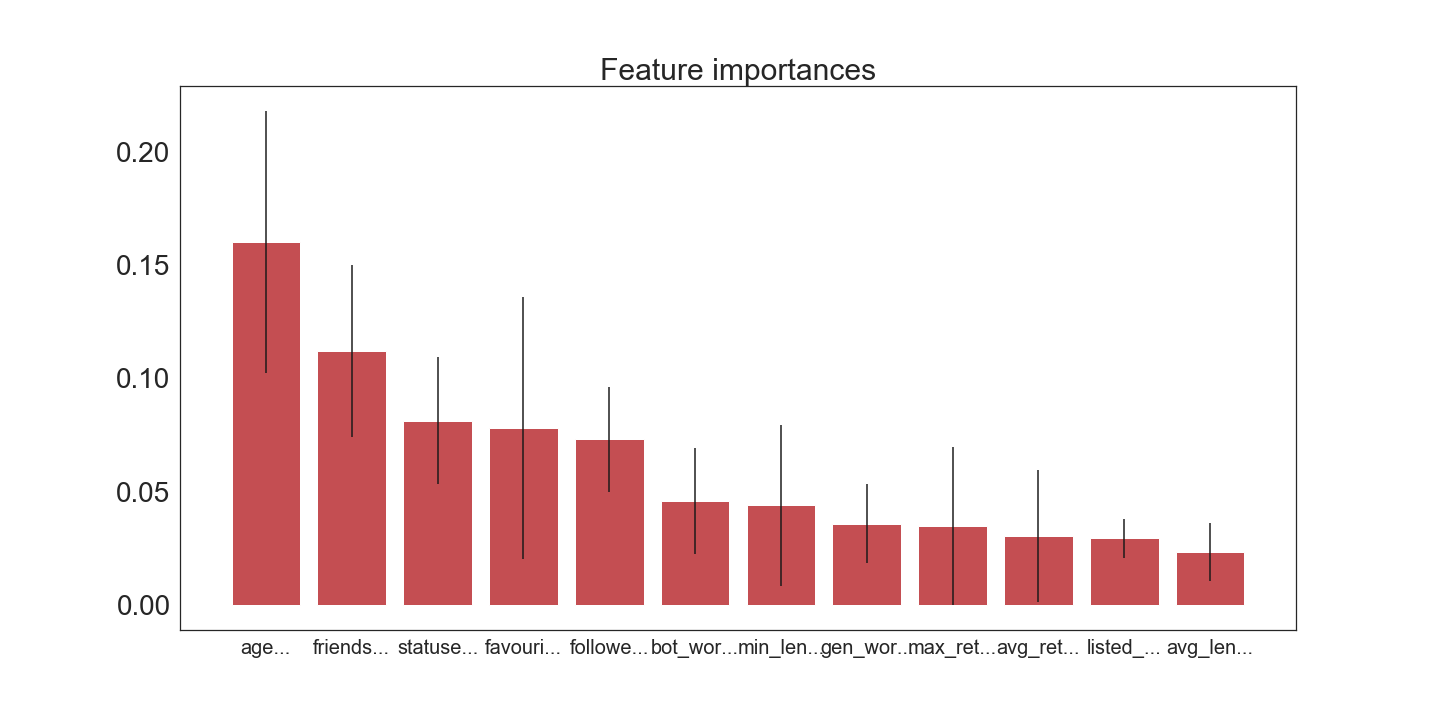
\includegraphics[width=\columnwidth]{chapter5/figure/bon_importances.png}
	\caption{Binary Random Forest features ranking}
	\label{fig:bon_importances}
\end{figure}

This was the first warning of a validation performance worsening.
A said before, the age of the accounts in the Caverlee's dataset were higher than the ones in our dataset. In particular, we examined the \textit{age} field of the training set, and the one coming from our validation samples, picked from the mutliclass dataset.
\begin{table}[!htb]
	\caption{Age field comparison among bot accounts}
	\begin{center}
		\begin{tabular}{@{}lr@{}}
			\multicolumn{2}{c}{\textbf{Training Bots}}\\
			\hline\hline
			\multicolumn{2}{c}{\textit{age}}\\
			\hline
			\multicolumn{1}{l}{mean}& \multicolumn{1}{r}{8}\\
			\multicolumn{1}{l}{std}& \multicolumn{1}{r}{0.66}\\
			\multicolumn{1}{l}{min}& \multicolumn{1}{r}{4}\\
			\multicolumn{1}{l}{max}& \multicolumn{1}{r}{12}\\
			\multicolumn{1}{l}{25\%}& \multicolumn{1}{r}{8}\\
			\multicolumn{1}{l}{50\%}& \multicolumn{1}{r}{9}\\
			\multicolumn{1}{l}{75\%}& \multicolumn{1}{r}{9}\\
			\hline\hline
		\end{tabular}
		\begin{tabular}{@{}lr@{}}
			\multicolumn{2}{c}{\textbf{Validation Bots}}\\
			\hline\hline
			\multicolumn{2}{c}{\textit{age}}\\
			\hline
			\multicolumn{1}{l}{mean}& \multicolumn{1}{r}{4.50}\\
			\multicolumn{1}{l}{std}& \multicolumn{1}{r}{2.69}\\
			\multicolumn{1}{l}{min}& \multicolumn{1}{r}{0}\\
			\multicolumn{1}{l}{max}& \multicolumn{1}{r}{11}\\
			\multicolumn{1}{l}{25\%}& \multicolumn{1}{r}{3}\\
			\multicolumn{1}{l}{50\%}& \multicolumn{1}{r}{4}\\
			\multicolumn{1}{l}{75\%}& \multicolumn{1}{r}{6}\\
			\hline\hline
		\end{tabular}
	\end{center}
	\label{table:bots}
\end{table}


\begin{table}[!htb]
	\caption{Age field comparison among genuine accounts}
	\begin{center}
		\begin{tabular}{@{}lr@{}}
			\multicolumn{2}{c}{\textbf{Training Genuine}}\\
			\hline\hline
			\multicolumn{2}{c}{\textit{age}}\\
			\hline
			\multicolumn{1}{l}{mean}& \multicolumn{1}{r}{9.22}\\
			\multicolumn{1}{l}{std}& \multicolumn{1}{r}{0.54}\\
			\multicolumn{1}{l}{min}& \multicolumn{1}{r}{4}\\
			\multicolumn{1}{l}{max}& \multicolumn{1}{r}{12}\\
			\multicolumn{1}{l}{25\%}& \multicolumn{1}{r}{9}\\
			\multicolumn{1}{l}{50\%}& \multicolumn{1}{r}{9}\\
			\multicolumn{1}{l}{75\%}& \multicolumn{1}{r}{9}\\
			\hline\hline
		\end{tabular}
		\begin{tabular}{@{}lr@{}}
			\multicolumn{2}{c}{\textbf{Validation Genuine}}\\
			\hline\hline
			\multicolumn{2}{c}{\textit{age}}\\
			\hline
			\multicolumn{1}{l}{mean}& \multicolumn{1}{r}{6.40}\\
			\multicolumn{1}{l}{std}& \multicolumn{1}{r}{1.94}\\
			\multicolumn{1}{l}{min}& \multicolumn{1}{r}{3}\\
			\multicolumn{1}{l}{max}& \multicolumn{1}{r}{11}\\
			\multicolumn{1}{l}{25\%}& \multicolumn{1}{r}{5}\\
			\multicolumn{1}{l}{50\%}& \multicolumn{1}{r}{6}\\
			\multicolumn{1}{l}{75\%}& \multicolumn{1}{r}{8}\\
			\hline\hline
		\end{tabular}
	\end{center}
	\label{table:genuine}
\end{table}

Like Tables \ref{table:bots} and \ref{table:genuine} show, there is a clear differences in the age attribute, between training and validation set.

We went forward to check if this diversity would had led us to a bad validation performance, or if the model would had handled the predictions in other ways.

The 10-fold crossvalidation on the validation set produced the following confusion matrix, with the correlated AUC score:\\

{
	\centering
	\begin{tabular}{@{}cc|cc@{}}
		\multicolumn{1}{c}{} &\multicolumn{1}{c}{} &\multicolumn{2}{c}{Predicted class} \\ 
		\multicolumn{1}{c}{} & 
		\multicolumn{1}{c|}{} & 
		\multicolumn{1}{c}{BOT} & 
		\multicolumn{1}{c}{GEN}  \\
		\cline{2-4}
		\multirow[c]{2}{*}{Actual class}
		& BOT  & 558 & 2442\\
		& GEN  & 158 & 2842\\
		\cline{2-4}
		\multicolumn{2}{r|}{AUC} & 
		\multicolumn{2}{l}{0.566}\\
		\multicolumn{4}{c}{}\\
	\end{tabular}\\
}
The worsening were real, and it highlighted the short-sighted training phase we performed, trying to top the Botometer performance.

We tried to mitigate this performance loss, by excluding the main suspect from the features set.
Here is the validation performance, without considering the accounts' ages.

{
\centering
\begin{tabular}{@{}cc|cc@{}}
	\multicolumn{1}{c}{} &\multicolumn{1}{c}{} &\multicolumn{2}{c}{Predicted class} \\ 
	\multicolumn{1}{c}{} & 
	\multicolumn{1}{c|}{} & 
	\multicolumn{1}{c}{BOT} & 
	\multicolumn{1}{c}{GEN}  \\
	\cline{2-4}
	\multirow[c]{2}{*}{Actual class}
	& BOT  & 2920 & 20\\
	& GEN  & 1589 & 1411\\
	\cline{2-4}
	\multicolumn{2}{r|}{AUC} & 
	\multicolumn{2}{l}{0.721}\\
	\multicolumn{4}{c}{}\\
\end{tabular}\\
}

The improvement was encouraging, but still not enough to rely on this basic solution.
Considering the bot target as the positive class, we still had too many False Positive in our confusion Matrix. The binary classifier used to tend to identify an user as a bot, with too much confidence. We had to reduce that number, in order to provide a reliable filter in the final prediction pipeline system.

\subsection{Data extension}
The idea we had was to use some data from our multi-class dataset to enrich the binary training set, in order to make the algorithm handle younger and different types of samples from the Twitter population.

In order to perform the extension, we sampled 3,000 genuine accounts and 8,000 bots (2,000 content polluters for each class), all coming from our dataset, and added them to the Caverlee's dataset.
The new training set was composed by 42,212 samples.

We performed a 10-fold-crossvalidation to see the effect of this data refill, sticking to the same hyperparameters found by the last Grid Search. The AUC score measured with these data was 0.963. We could see a slight improvement of the performances, with this data extension. However, we wanted to take a look inside the inner ranking performed by the algorithm, to check if the age field represented an important splitting point.
Figure \ref{fig:bon_importances_ext} shows that the age attribute was still the most considered when the trees had to perform the first splits.

We couldn't blindly follow the AUC score through Grid Searches, without making considerations about what will happen when we will allow people to classify data coming from outside our collected samples.
The age feature would have driven the Random Forest to misclassification over accounts with low \textit{age} values.
Even if the exclusion of that attribute would had made the overall AUC score worse, we had to strip it from the features vector, in order to better generalize on real test cases.

\begin{figure}[htp!]
	\centering
	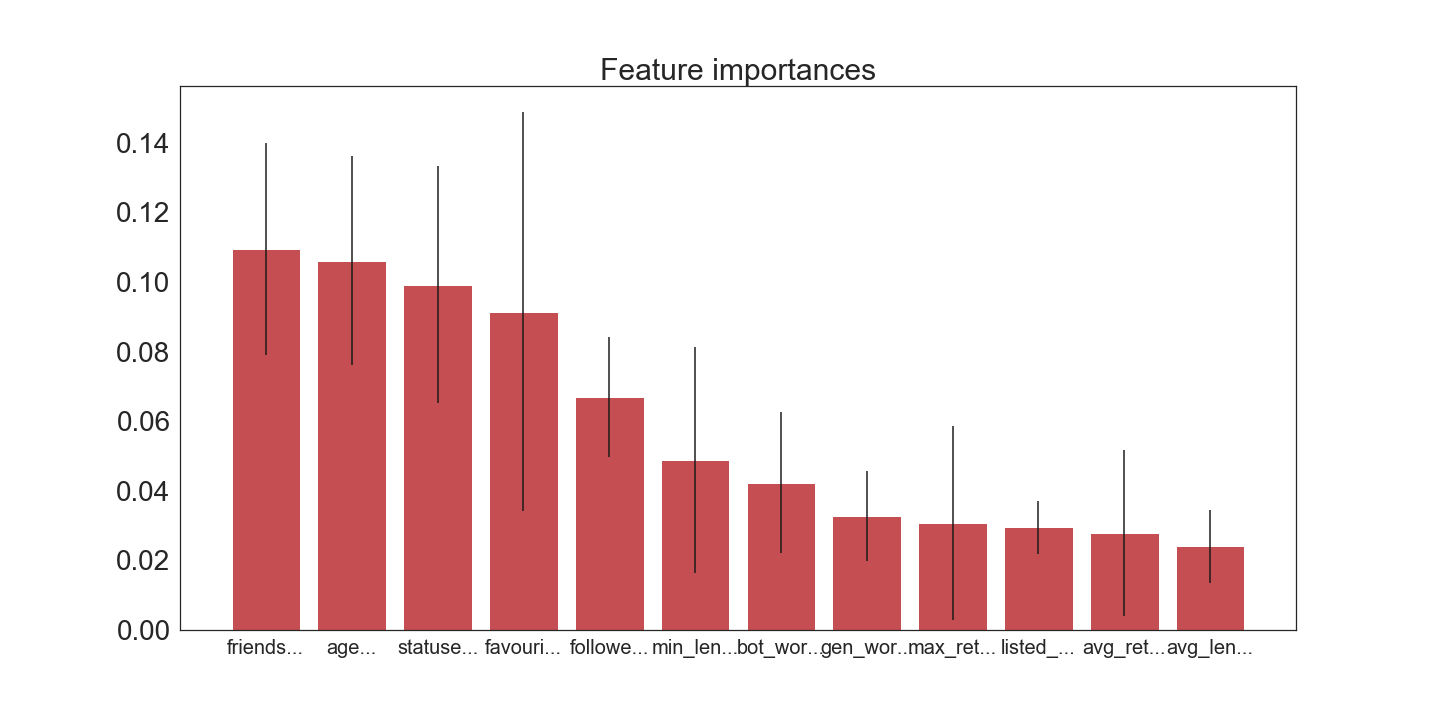
\includegraphics[width=\columnwidth]{chapter5/figure/bon_importances_extensions.png}
	\caption{Features ranking with augmented data - Top 12 }
	\label{fig:bon_importances_ext}
\end{figure}

While cross-validating the model, we tested the complete features vector (with and without the extension from our dataset) and the one stripped by the age values. The crossvalidation was performed with the same hyperparameters settings of the model fitted with the Caverlee's dataset only.

{
	\centering
	\begin{tabular}{@{}cccc@{}}
		\multicolumn{1}{c}{} & 
		\multicolumn{3}{c}{Fitted data} \\ 
		\cline{2-4}
		\multicolumn{1}{c|}{} & 
		\multicolumn{1}{c|}{original - with \textit{age} } & 
		\multicolumn{1}{c|}{extended - with \textit{age} } & 
		\multicolumn{1}{c|}{extended - without \textit{age}} \\
		\cline{1-4}
		\multicolumn{1}{|c|}{AUC} & 
		\multicolumn{1}{c|}{\textbf{0.961}} & 
		\multicolumn{1}{c|}{\textbf{0.963}} & 
		\multicolumn{1}{c|}{\textbf{0.948}} \\
		\cline{1-4}\\
	\end{tabular}\\
}

The age filed removing made thing worse, but we decided to perform it anyway, because of the good score reached without it, and the flexibility we were giving to the Random Forest. The slight worsening could be also imputed to the biased extrinsic features of that data: those samples came from the multi-class dataset and they originally had the extrinsic features based on the four bot categories' dictionaries.
In order to refill the binary dataset with these new samples, we had to recompute the extrinsic features, applying the analogous method used for the binary purpose.
We didn't recompute the entire dictionaries, we just assigned the scores to the new samples we were introducing, basing the calculations on the already listed words. Those had been exposed in chapter \ref{capitolo4}. This approach aimed to force the algorithm to identify bots and humans, basing its comparisons on the online computations of those features, like in a real-case generalization.

This last configuration was used to performed a further tuning of the parameters.
A new Grid Search brought us the configuration for the hyperparameters shown in Figure \ref{fig:bon_tuning_refil}, leading to the new AUC score, exposed in Figure \ref{fig:bon_refil_auc}.
\begin{figure}[htp!]
	\centering
	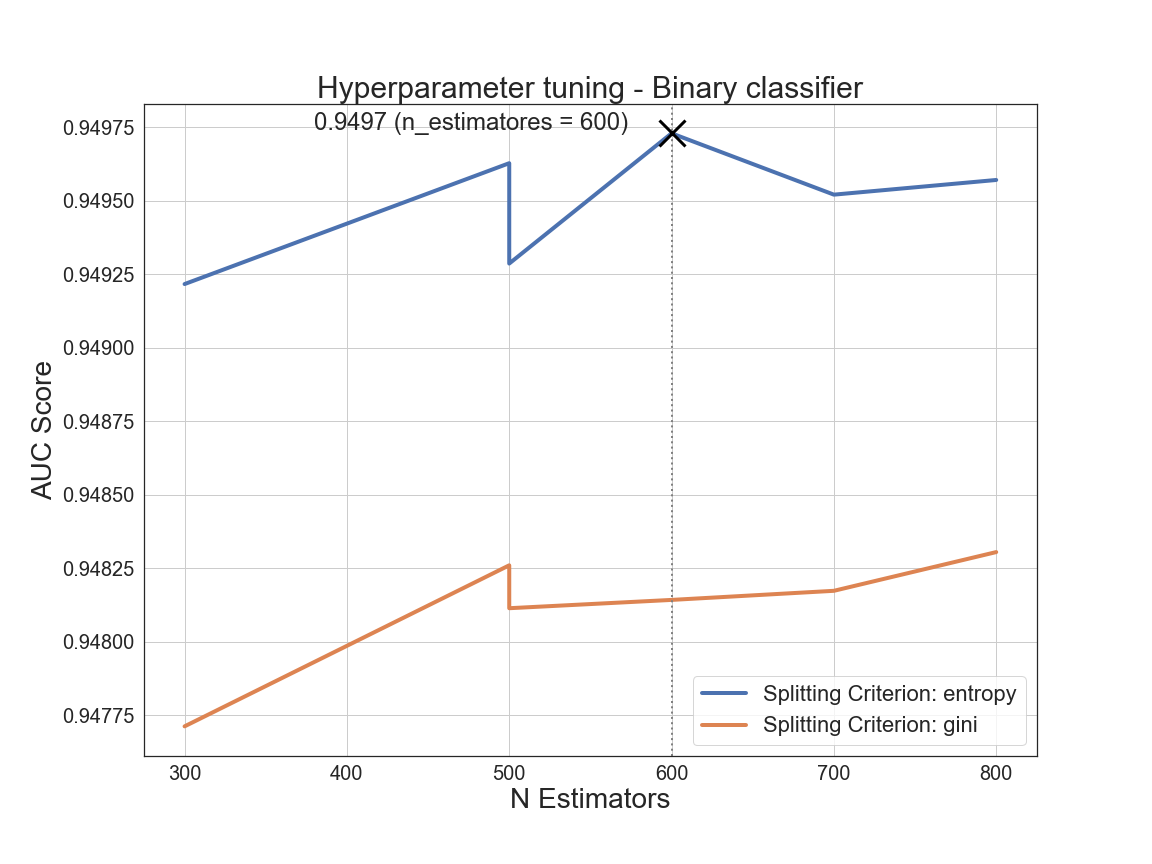
\includegraphics[width=\columnwidth]{chapter5/figure/bon_tuning_refill.png}
	\caption{Grid Search with extended data}
	\label{fig:bon_tuning_refil}
\end{figure}
\begin{figure}[htp!]
	\centering
	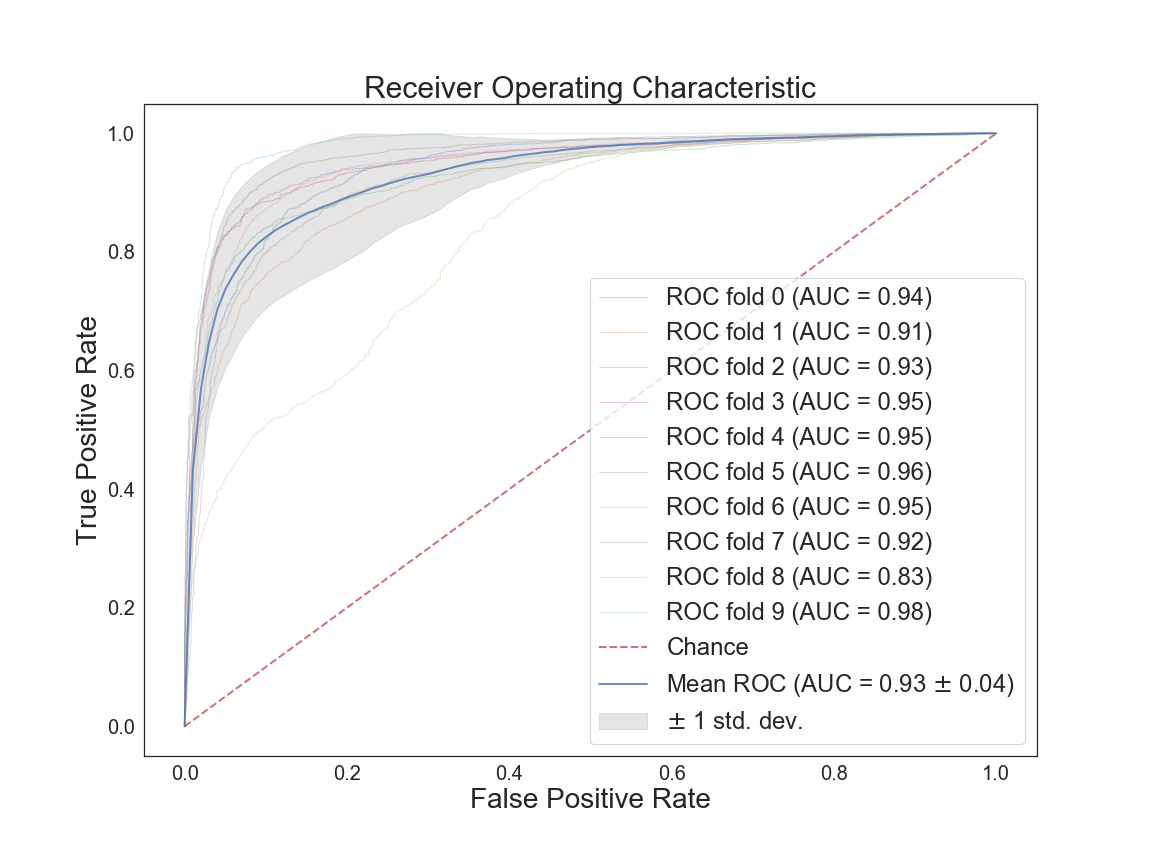
\includegraphics[width=\columnwidth]{chapter5/figure/refill_auc.png}
	\caption{AUC score with extended data}
	\label{fig:bon_refil_auc}
\end{figure}
The binary classifier has then been fitted with 42,212 samples with 34 features, 600 estimators, entropy splitting criterion and 26 levels of maximum depth.

\section{Multi-class ensemble classifier}
It somehow represents the core of our thesis, it models the starting idea: go deep inside bot identification and search and classify similar behaviours among them.

In this section we will expose the model involved in the multi-class ensemble. In this process, we used a Random Forest algorithm, working on all the crafted features; a KNN model, operating on the user attributes only; a final text-based Naive Bayes classifier, which reads the tweets' texts and classifies them.

At first, this ensemble of these three models should have been blended with the prediction of the binary classifier. That means that the genuine class was part of the labels we were trying to classify, even in the multi-class models. Then, we found an issue in this approach: the binary classifier itself wasn't enough, even including it into the ensemble, to give the right importance to the genuine accounts. This problem emerged because of the others classifiers, as they were trying to classify the genuine class too. They lacked in data with that target, so, basically, they used to treat that category as one other of the bot types.

Even if the results on our validation sets were still good (we accomplished a F1 measure of 0.973), for the final ensemble method, we knew that this method would had yielded to a poor bot vs genuine detection tool. We couldn't accept that situation, because, in order to go deeper than other works, in bot behaviour classifications, we had to provide a solid previous discrimination between humans and automated accounts.

The ensemble method with all the classifiers blended together were replaced with a pipeline, and the multi-class models were trained on bot categories only.
These last classifiers had been put together inside a  ensemble, which returns the final mutliclass probability prediction, based on the opinions of those models, as shown in Figure \ref{fig:stacking_schema}

The different nature of the classifiers, and the feature subsets as well, is one of the strengths of the stacking approach: it combines different opinions about the samples, driven by different classifiers, considering different parameters and attributes; basing on those unlike classifications, it builds its own.

It differs from other ensemble methods as bagging and boosting, because of this miscellaneous schema, and it can be a robust method to exploit the different characteristics of the classifiers stacked together.

\begin{figure}[htp!]
	\centering
	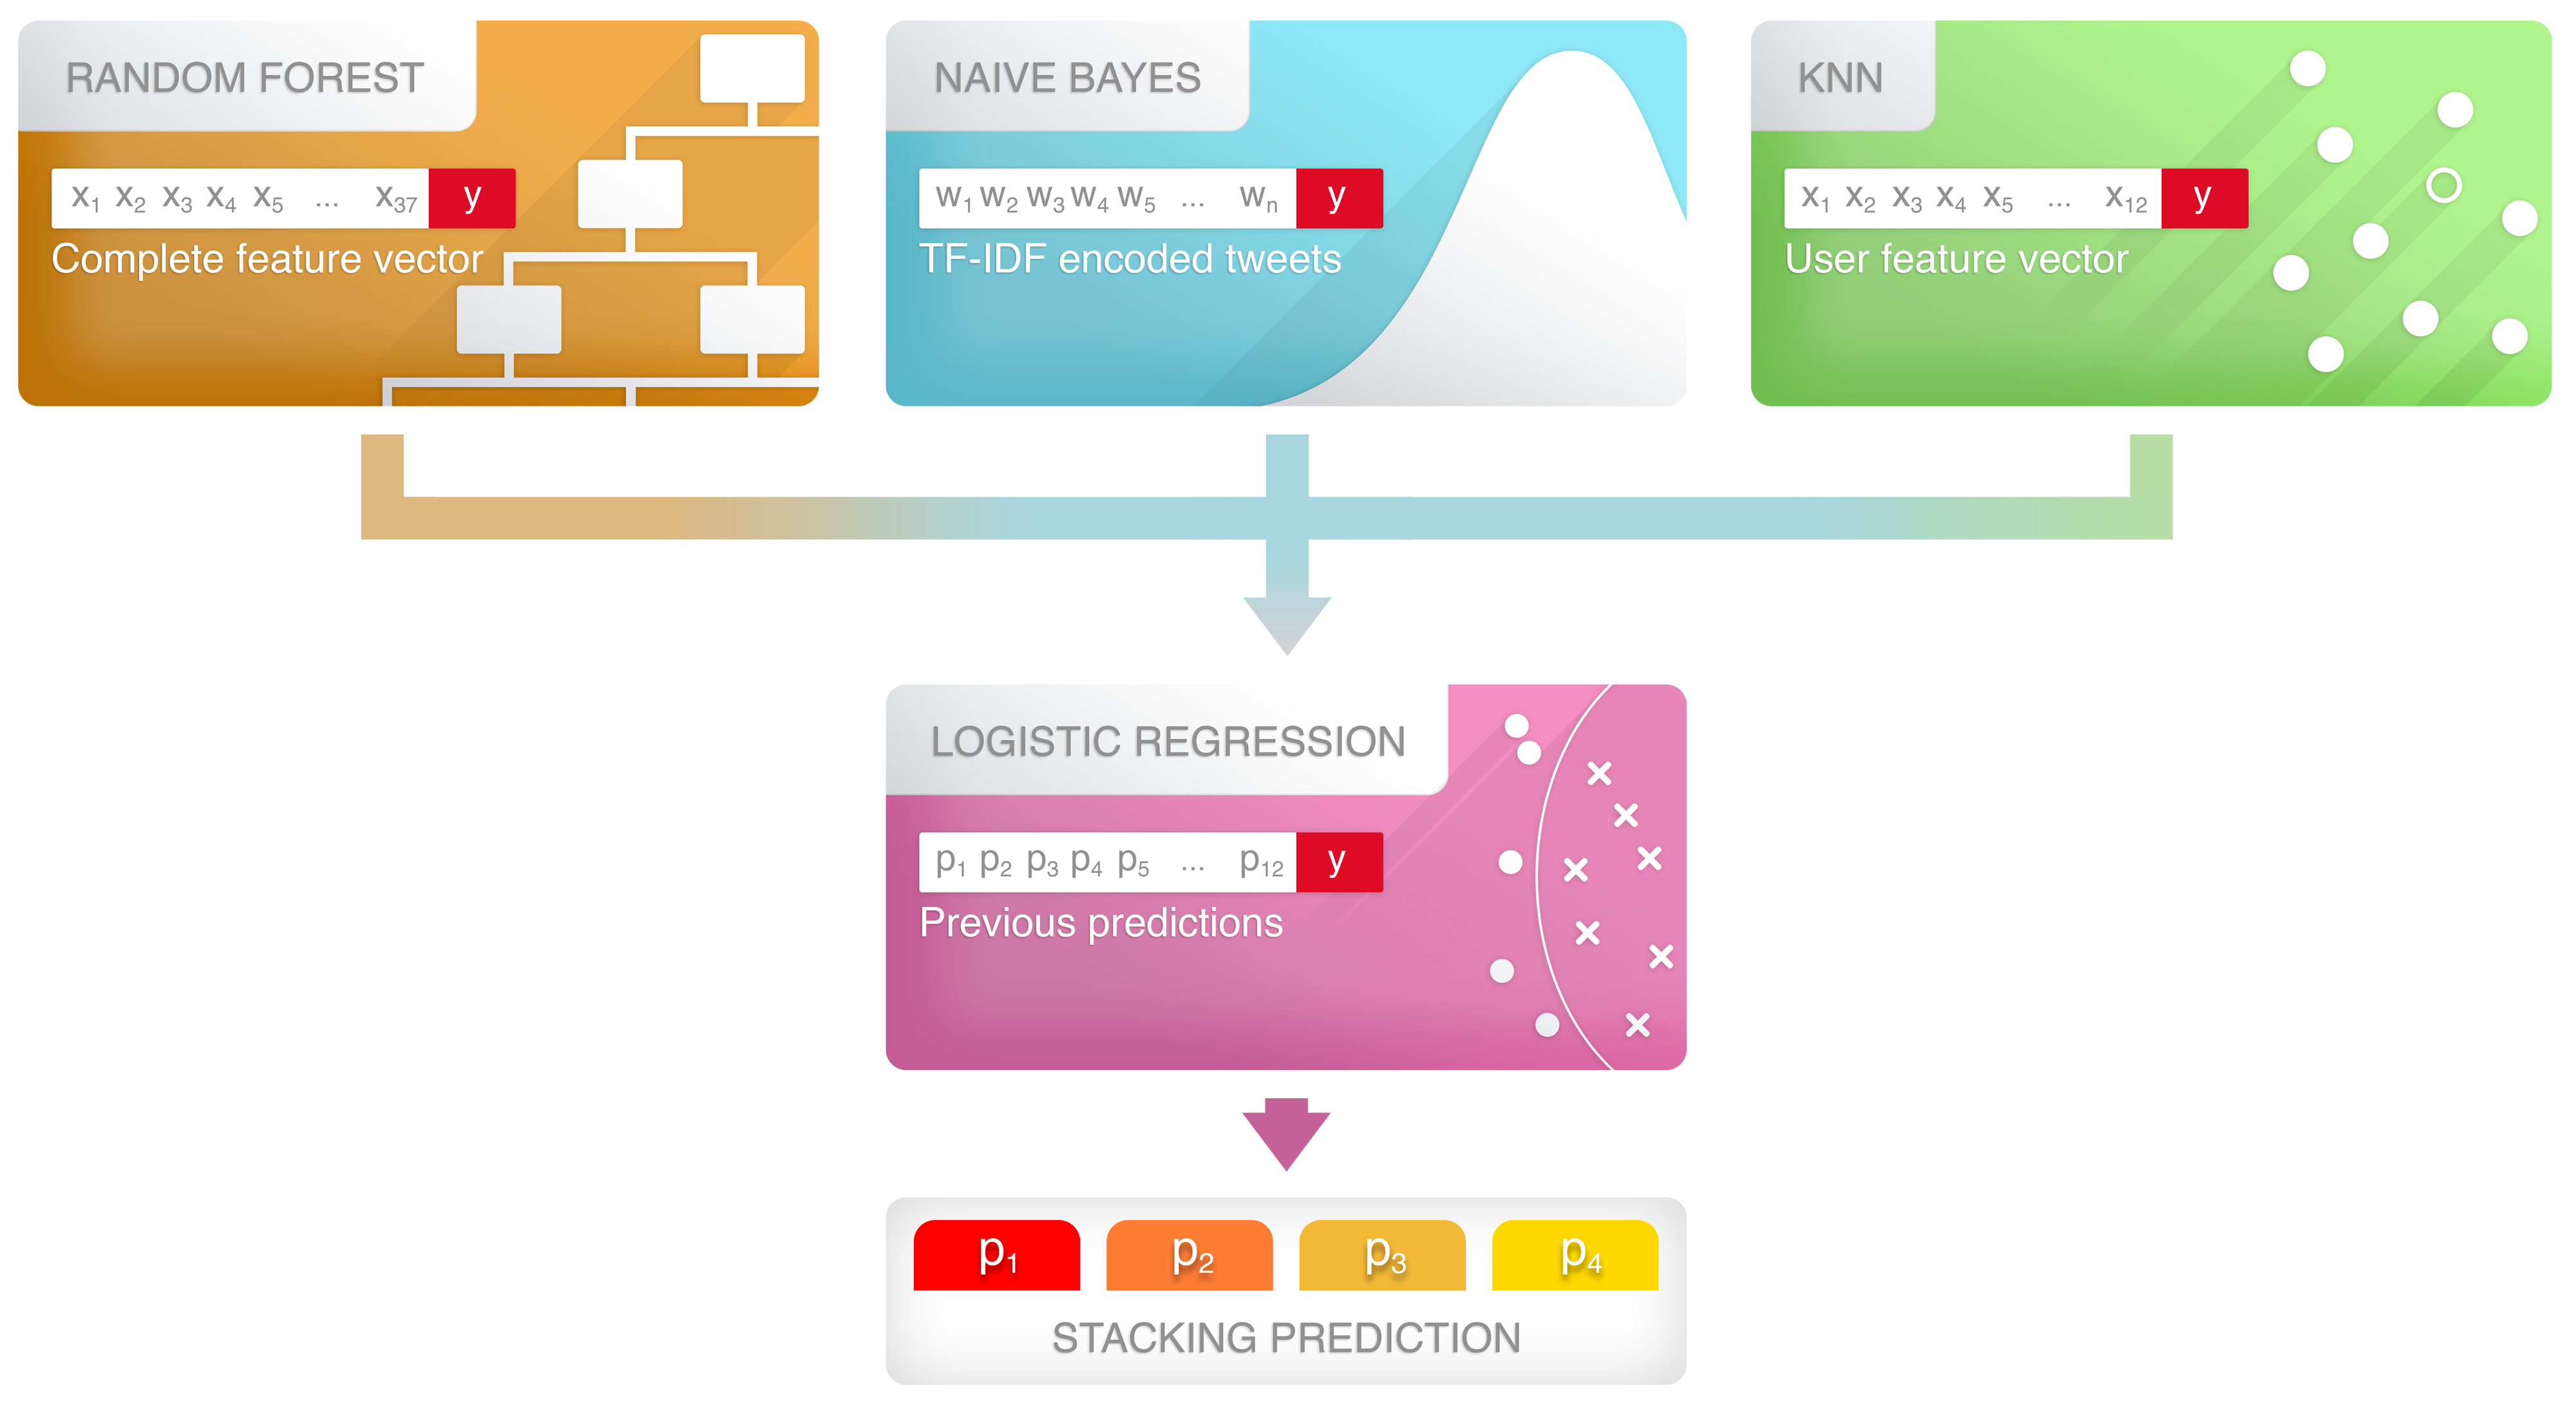
\includegraphics[width=\columnwidth]{chapter5/figure/stacking.png}
	\caption{Multi-class ensemble schema}
	\label{fig:stacking_schema}
\end{figure}
In the following subsections there are the detailed explanations of the three classifier announced before.

\subsection{All-features-based Random Forest classifier}
\subsubsection{Dataset}
During this phase, we used the previously described dataset \ref{sec:dataset} with its four different labels.
The algorithm was fed with 21,445 samples and 37 features. the amount of records were light enough to consider K-fold crossvalidation, without slow the validation down too much.
\subsubsection{Model}
We found ourselves in the situation in which we had some brand new features and we didn't know how useful they were. Obviously, we could appeal to heat-maps or other tools, to highlight the correlations among variables and targets.
However, the model we wanted to develop was the Random Forest, which proved to perform well with F1 score. Since this kind of model exploits its criteria to employ the features, we needed to prove them with a direct approach.

\subsubsection{Features selection}
A useful advantage of the Random Forest algorithm is the ability to provide a feature ranking, according to its splitting criterion.
We retrieved this standing, in order to see if we would have found some of the ones coming out from feature engineering at the top positions.
The algorithm ranking ranked the features this way: 1. \textit{favourites\_count} (0.179), 2. \textit{nsfw\_profile} (0.068), 3. \textit{freq} (0.061), 4. \textit{tweet\_intradistance} (0.060), 5. \textit{news\_spreaders\_words\_score} (0.058), 6. \textit{statuses\_count} (0.053), 7. \textit{avg\_len} (0.051), 8. \textit{followers\_count} (0.051), 9. \textit{NSFW\_words\_score} (0.043), 10. \textit{ret\_perc} (0.041), 11. \textit{min\_len} (0.038), 12. \textit{spam\_bots\_words\_score} (0.035), ...  37. \textit{min\_fav} (0.0001).

\begin{figure}[htp!]
	\centering
	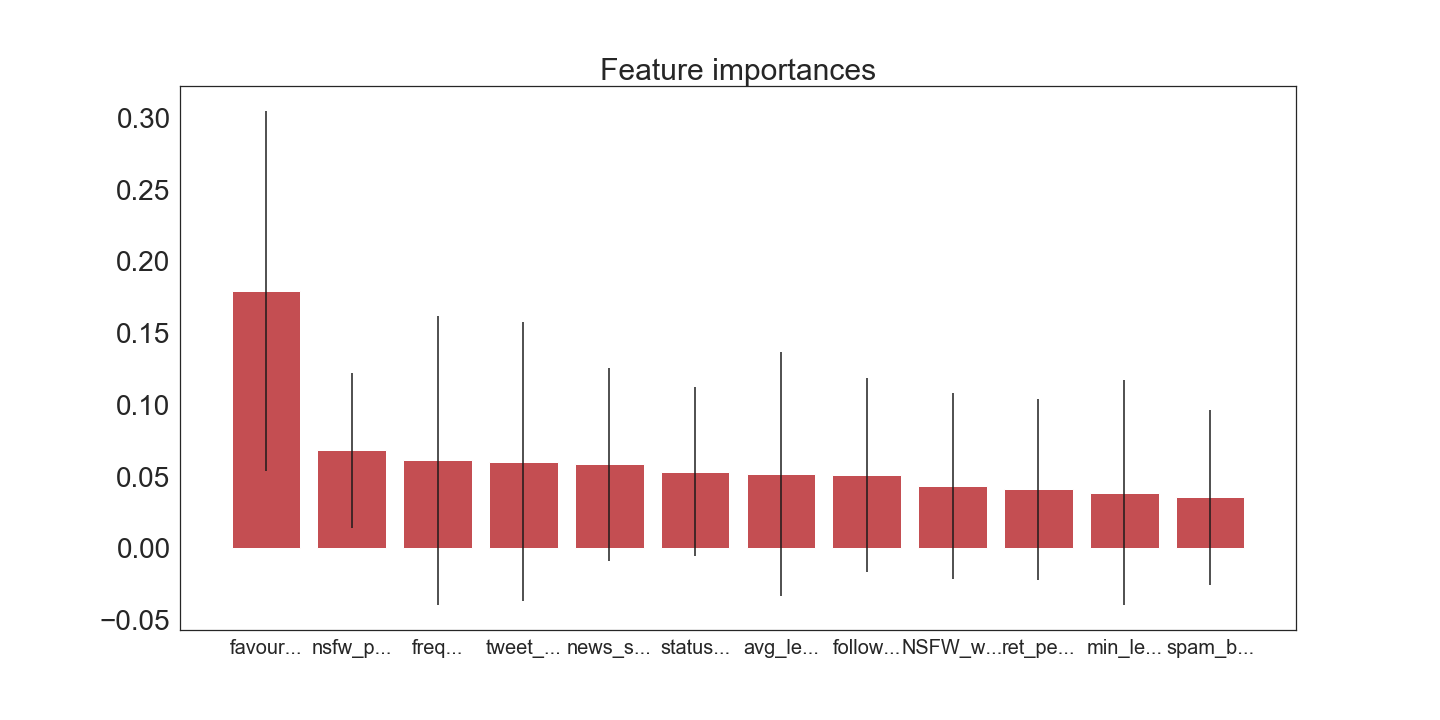
\includegraphics[width=\columnwidth]{chapter5/figure/top_12_features_importances.png}
	\caption{Random Forest top-12 feature ranking}
	\label{fig:feature_rank}
\end{figure}

As Figure \ref{fig:feature_rank} shows, we could find some of our crafted features inside this list: lots of tweets descriptive features (\textit{avg\_len, freq, ret\_perc}, etc...), as well as the \textit{tweet\_intradistance} attribute and three of the four extrinsic features, like \textit{news\_spreaders\_words\_score}, \textit{NSFW\_words\_score} and the \textit{spam\_bots\_words\_score}.
This picture confirmed us that the idea behind those features was useful.

Since those attributes were thought to belong to different clusters, we decided to try several combinations of those feature clusters, validating the model on them with a crossvalidation. The purpose of this stage was to see if some groups of features were enough to describe the real problem, or if some group would shown up as irrelevant.
To face this evaluation, we performed a light-weighted Grid Search, which is a method that takes desired ranges of hyperparameters and tries all the possible permutations of them, looking for the best combination, in terms of a certain metric.

We are talking about a light-weight version of this tool, because we just went through different numbers of tree estimators in the forest. The different feature groups are not considered as hyperparameters and are not handled by the Scikit-learn implementation of the Grid Search.
We had to manage the different training by our own, looking how the test score would have changed along with the increasing number of estimators and the different set of features.

Grid Search uses crossvalidation to find the better estimators for the models, and this approach was right for our situation.
Due to the multi-class nature and some imbalances with the labels, we decided to follow the F1 score metric to asses the value of our model.

The features were organized in clusters, as described in Chapter \ref{capitolo4}.
We had the user features, the descriptive features, the intrinsic features, the extrinsic and the image features. Then we tried the model with the entire set of 38 attributes.
As shown in Figure \ref{fig:feature_clusters}, the best configuration seems to involve the whole set of features, as it reaches these scores, with 100 estimators: \textit{Precision} = 0.978, \textit{Recall} = 0.976, \textbf{\textit{F1}}= 0.977.

\begin{figure}[htp!]
	\centering
	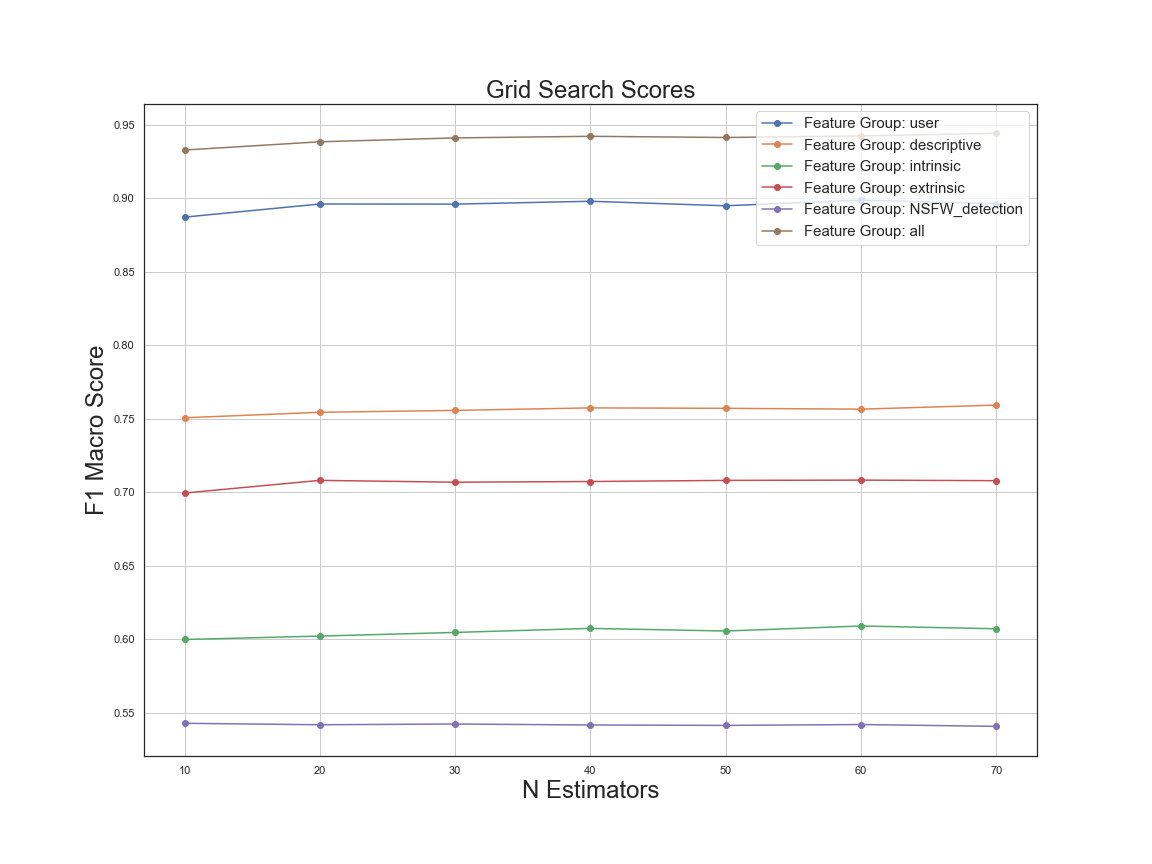
\includegraphics[width=\columnwidth]{chapter5/figure/feature_cluster_f1.png}
	\caption{Performance over different feature clusters}
	\label{fig:feature_clusters}
\end{figure}

The model has been tested with the default value for the maximum depth in the trees, which is set to 'None'. It means that the trees are expanded until every leaf is pure, or all leaves contain one sample.

In order to try all the alternatives, we setted a test involving the performance of the model, when it was working on an increasing number of features.
We had the ranking provided by the forest itself, so we started by testing only the most important attribute, adding one feature at time, until the least important was included.
We were looking for some changing in the scores, that would have pointed to a lighter model, with the exclusion of some features.
Figures \ref{fig:feat_prec}, \ref{fig:feat_rec}, \ref{fig:feat_f1} show the trends of the Precision, the Recall and the F1, respectively, along with the number of features tested.
 \begin{figure}[htp!]
 	\centering
 	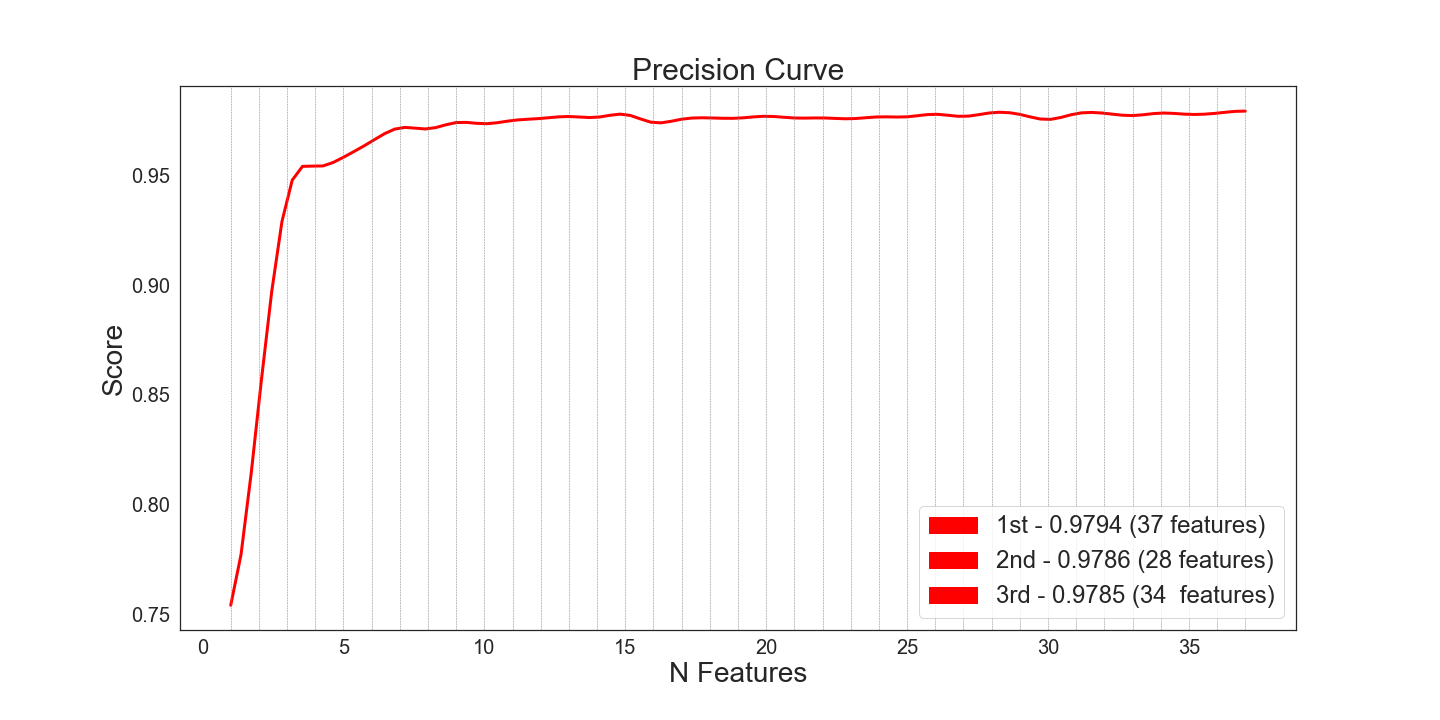
\includegraphics[width=\columnwidth]{chapter5/figure/precision_along_features.png}
 	\caption{Precision trend along with number of features tested}
 	\label{fig:feat_prec}
 \end{figure}
\begin{figure}[htp!]
	\centering
	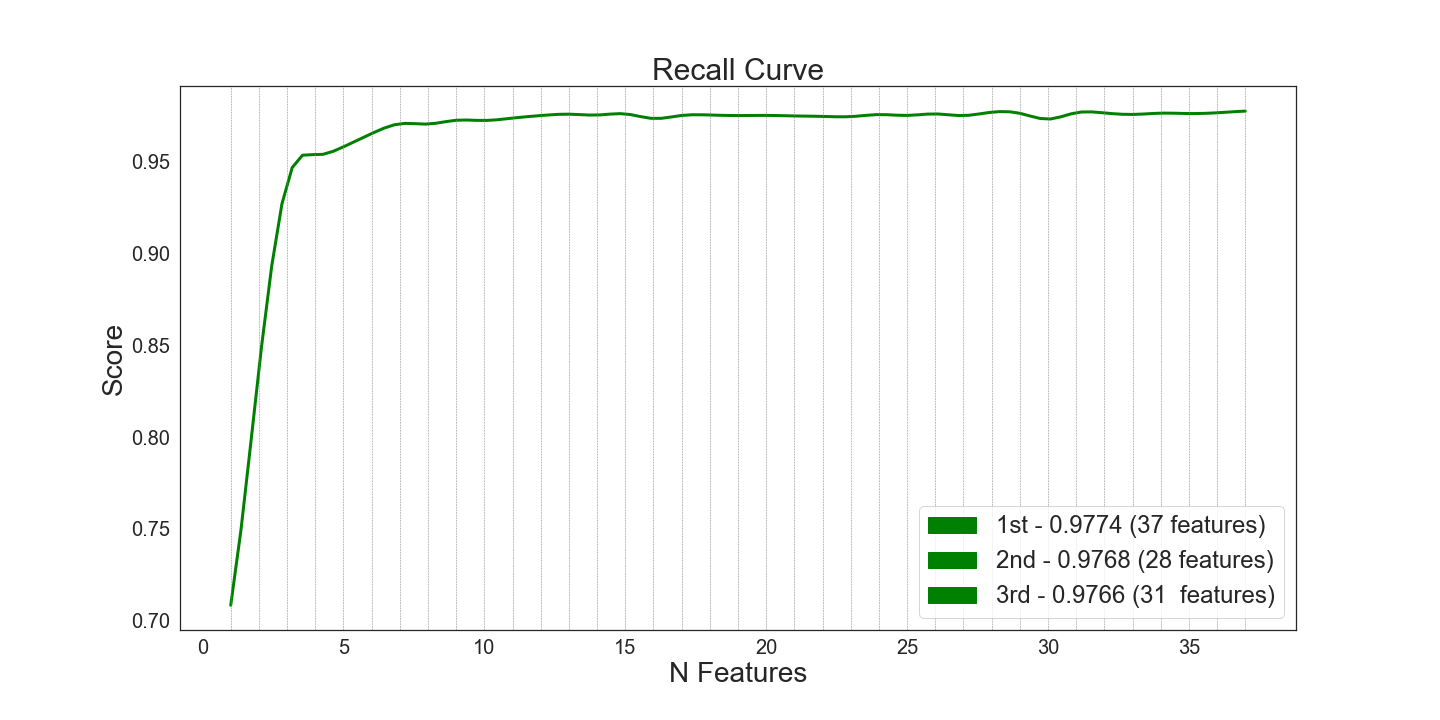
\includegraphics[width=\columnwidth]{chapter5/figure/recall_along_features.png}
	\caption{Recall trend along with number of features tested}
	\label{fig:feat_rec}
\end{figure}
\begin{figure}[htp!]
	\centering
	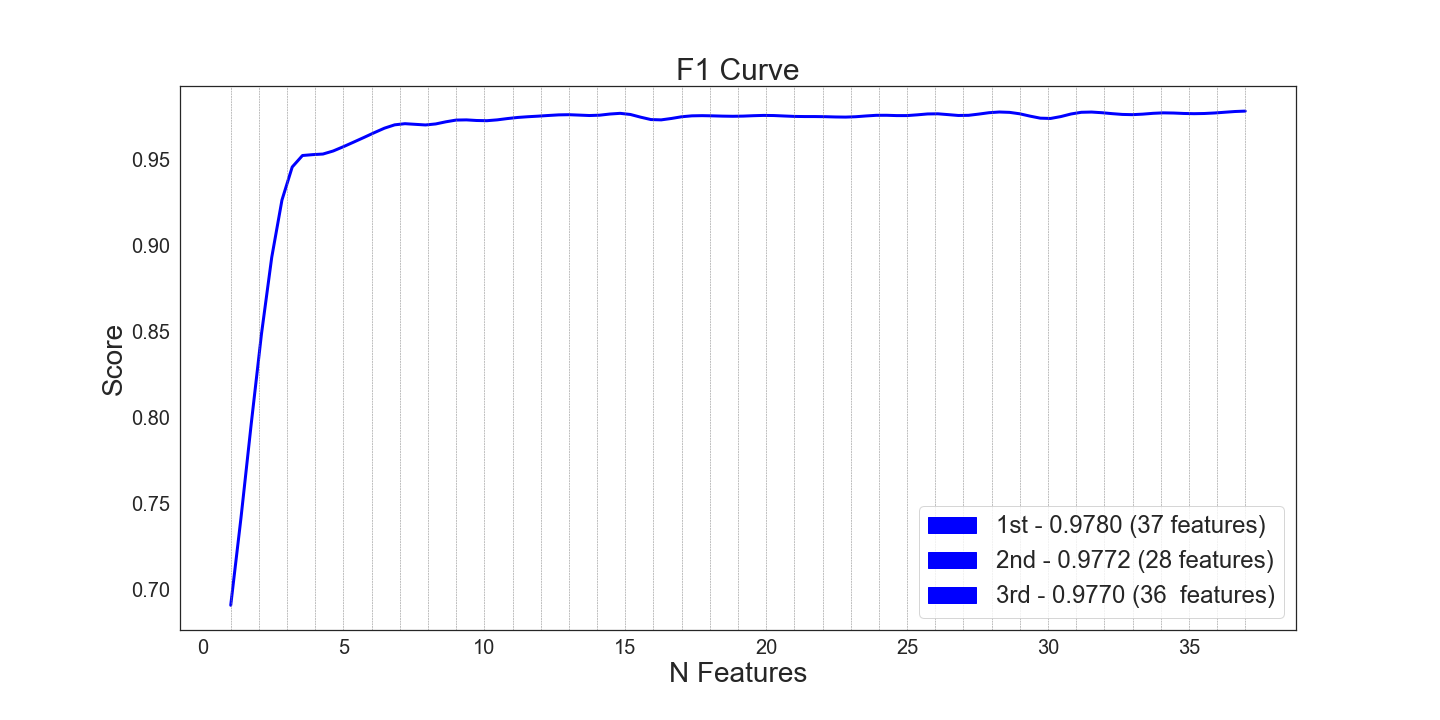
\includegraphics[width=\columnwidth]{chapter5/figure/f1_along_features.png}
	\caption{F1 trend along with number of features tested}
	\label{fig:feat_f1}
\end{figure}

As all the Figures show, the best solution possible, looking at both the three metrics, is the one involving all the 37 components of the feature vector.
There was the possibility to choose the second result, which wanted only the first 28 features, in terms of importance for the Random Forest. However, we weren't struggling with heavy models or long prediction times and the Random Forest algorithm handles the overfitting problem properly, even with complex models.
Thus, we moved on with the entire feature vector as support for the classification goal.

We then continued with a proper Grid Search over the whole number of features.
\subsubsection{Hyperparameters Tuning}
The algorithms rely on parameters in order to fit a problem.
Once the number of featured was picked, as well as the model, we needed to consider the possible hyperparameter ranges. 
The Grid Search method from Scikit-learn helped us, once again, during this exploration.
Since we were testing a Random Forest, we wanted to play with the number of estimators (tree) to include in the pool, as well as the maximum depth of each tree and the splitting criterion.

\begin{figure}[htp!]
	\centering
	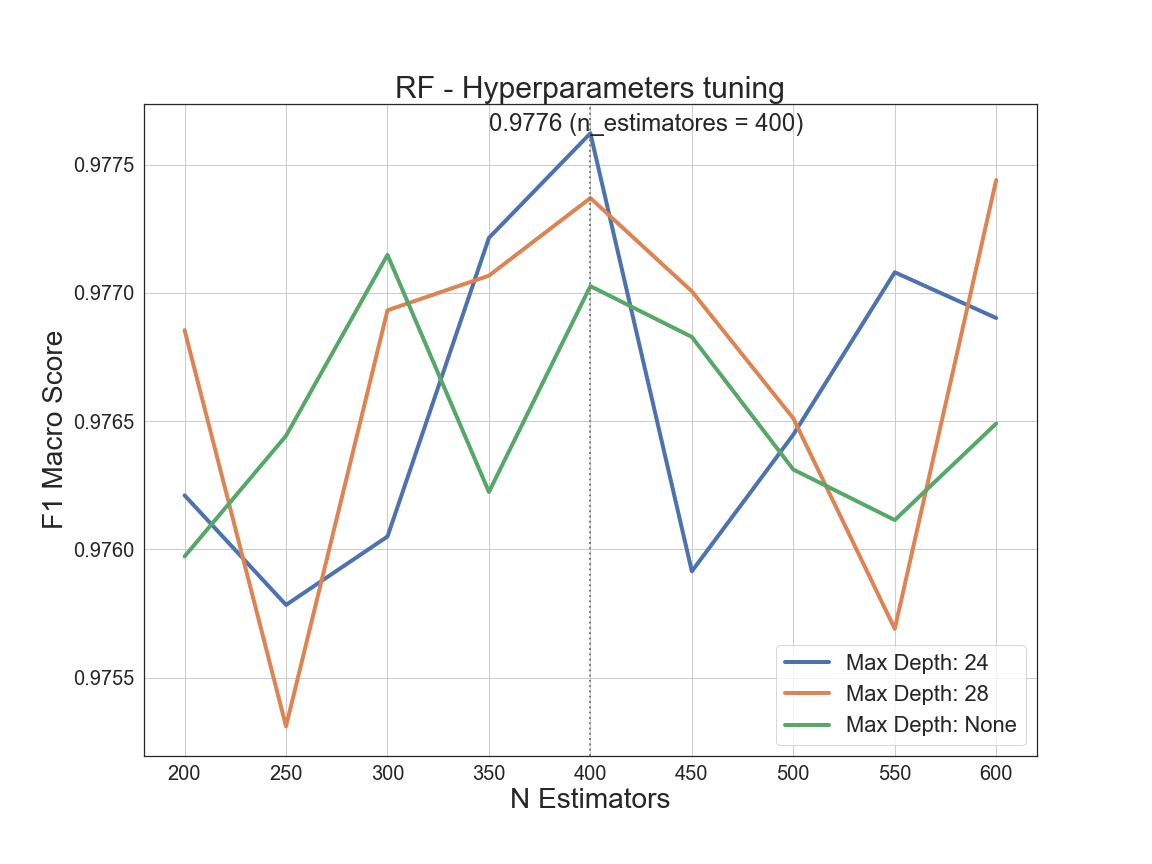
\includegraphics[width=\columnwidth]{chapter5/figure/multiclass_rf_tuning_gini.png}
	\caption{F1 scores with ``Gini`` criterion - close-up view}
	\label{fig:rf_tuning_gini}
\end{figure}
\begin{figure}[htp!]
	\centering
	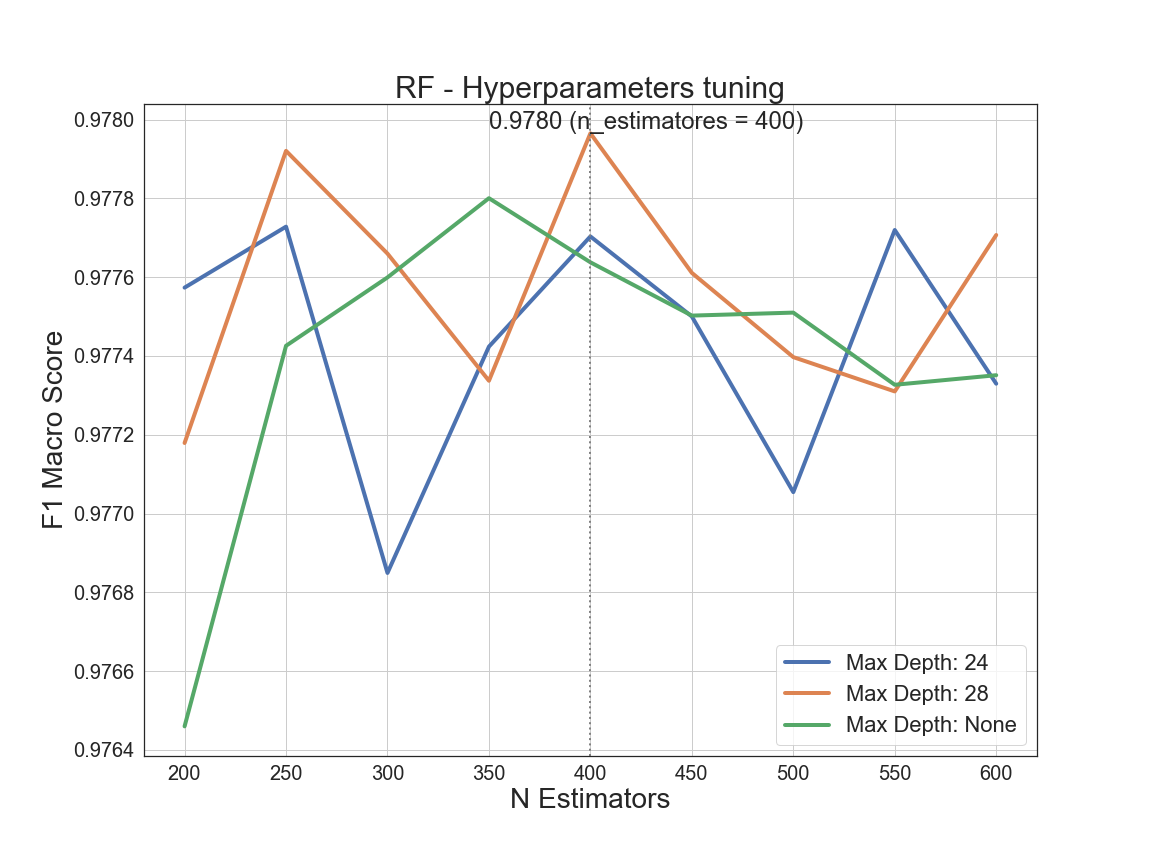
\includegraphics[width=\columnwidth]{chapter5/figure/multiclass_rf_tuning.png}
	\caption{F1 scores with ``Entropy`` criterion - close-up view}
	\label{fig:rf_tuning_entropy}
\end{figure}

The Figures \ref{fig:rf_tuning_gini}, \ref{fig:rf_tuning_entropy} show how the average F1 score, measured on 10-fold crossvalidation, changes with the increasing of the number of estimators in the forest.
The different coloured lines represent the \textit{max\_depth} hyperparameter.
The first Figure (\ref{fig:rf_tuning_gini}) shows the Grid Search results, with the \textit{gini} splitting criterion.
The second one (\ref{fig:rf_tuning_entropy}) represent the situation having \textit{entropy} as a splitting choice.
We combined nine numbers of estimators (200, 250, 300, 350, 400, 450, 500, 550, 600), together with three different maximum depths for the trees (26, 28, None) and the two above-mentioned splitting criteria.

We could observe a peak, for both criteria, in correspondence with 400 estimators.
Although the Gini-based forest's score didn't seem a bad point, we went with the Information Gain splitting criterion, which si also the same we used to rank the features of our data.

The final configuration involves 400 trees, the Information Gain criterion and the maximum reachable depth (for each of the 400 estimators) equal to 28 levels, yielding the following scores in 10-fold-crossvalidation:
\begin{itemize}
	\item[\PencilRight] \textit{Precision}: \textbf{0.979}
	\item[\PencilRight] \textit{Recall}: \textbf{0.977}
	\item[\PencilRight] \textit{F1 score}: \textbf{0.978}
\end{itemize}

Figure (\ref{fig:tree}) shows an example of one of the estimators of the final model, plotted with Matplotlib library for Python. It has been represented with the first two levels of depth, for visualizations reasons.

\begin{figure}[htp!]
	\centering
	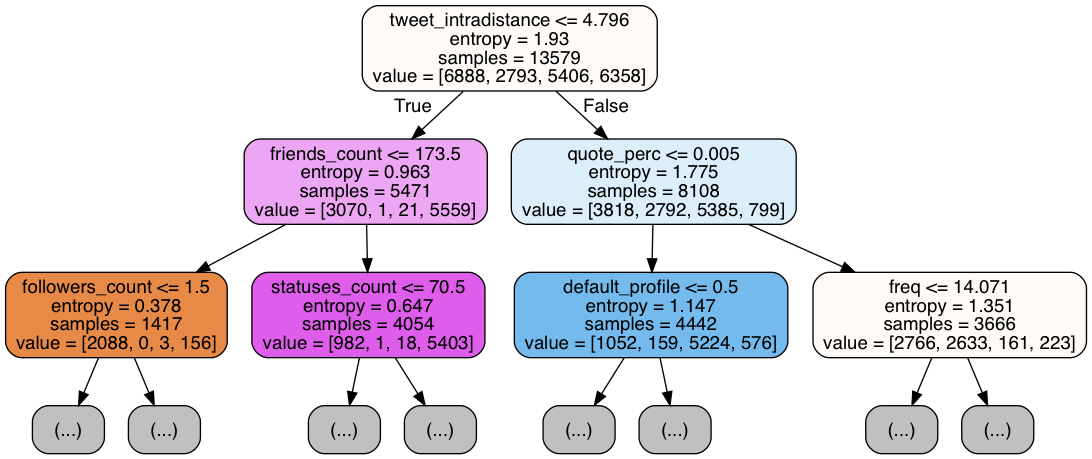
\includegraphics[width=\columnwidth]{chapter5/figure/tree.png}
	\caption{Tree estimator of the Random Forest model}
	\label{fig:tree}
\end{figure}

As the picture shows, this tree used the \textit{tweet\_intradistance} feature as root, in order to perform its first split on that attribute.

The first algorithm of the multi-class ensemble was completed and ready to be combined with the following models.

\subsection{User-based KNN classifier}
The Random Forest model represents somehow the core of the ensemble, as it was trained on the entire feature vector, with all the data we had for the purpose. A massive attention for parameters and features were given for that classifier. 
However, we wanted to put it into an ensemble, not to improve its already strong stability over outliers, but to support it with different perspectives.

We noticed, as shown in the previous Figure \ref{fig:feature_clusters}, that the user features were a good group to build a classifier on. Thus, we started thinking how to implement such support, and we basically looked at our baselines.

The model that had the best performance, not considering the Random Forest, was the K-Nearest Neighbors algorithm.

We didn't want this model to work the entire feature vector, because we knew that it would had been overlooked by the Random Forest. Instead, we wanted it to concentrate on the features that describe the users, without the information driven by their tweets. Therefore, we relied on the user features, with the extension of the image feature that assesses the NSFW score to the profile picture. This extension wa due to the fact that such feature doesn't need the user's tweets to be computed; it can be seen as one of the user features as the others of that group.

We hoped that treating the data before, or during, the training phase, would had brought to a good sustain for the first multi-class model, where needed.

\subsubsection{Dataset}
The dataset is composed of the same number (21,445) of samples of the first multitarget Random Forest, but preserving only the twelve features belonging to the user group, plus the NSFW\_profile attribute coming from the image features group.

\small
\begin{center}
	\begin{tabular}{ll}
		\\Feature vector\\
		\hline\hline
		default\_profile, favourites\_count, followers\_count\\
		friends\_count, listed\_count, screen\_name\_len\\
		statuses\_count, url, description\_len, NSFW\_profile\\
		name\_len, profile\_use\_background\_image, age\\\hline\\
	\end{tabular}
\end{center}
\normalsize

\subsubsection{Model}

This model is quite simple and doesn't require much effort in interpolating several hyperparameters. But this doesn't mean that it is a closed box algorithm. It can be improved by paying attentions to some details. In particular there had been done three considerations, and they were regarding

\begin{itemize}
	\item[\PencilRight]\textbf{Hyperparameters}\\
	The main hyperparameters that can be combined together are the number \textit{k} of neighbours ti consider, when performing a prediction, and the distance metric used by the calculations of the distances.
	The Scikit-learn implementation of the algorithm uses the \textit{Minkowski} metric, which describes the \textbf{L}\textsubscript{p} norm: 
	\[ \mathit{L_{p}} = (\sum\limits_{i = 1}^{n}|x_{i} - y_{i}|^{p})^{1/p} \]
	This metric is a generalization of the \textbf{L}\textsubscript{2} norm, also known as the Euclidean distance.
	The library we used allowed us to tune the \textit{p} hyperparameter, which indicates the metric used: \textit{p} = 1 means L\textsubscript{1} norm, the Manhattan Distance, when \textit{p} = 2 stands for the Euclidean.
	Higher values of \textit{p} are available, with other metric involved.
	
	We tried several values for both \textit{p} and \textit{k}, obtaining different results.
	However, the overall decision had to take in consideration also other two factors, the features weighting and the kernel function.
	
	\item[\PencilRight]\textbf{Features Weighting}\\
	The KNN algorithm aims to map the samples into a space and then it looks for the distances among them. In order to have best mapped space, it is reasonable to perform a weighting over the data. With this approach, the mapping would change and some points could result both as closer or more distant from each others.
	
	We performed some tests on four configurations. The first one didn't involve a weighting vector, while the second one was a standard normalization of the features.
	This last option provided weak results, with the same configurations of parameters, and thus were discarded from further analysis.

	The third option, which was the most interesting, was built by computing the Information Gain for each feature, using the inner ability of the Random Forest classifier, and then by applying the weights on the attributes, basing the coefficients on the scores provided by the ranking.
	This method emerged as the most effective, in the overall score.
	
	The last one was implemented as a Gaussian Kernel, which exploits the above-explained Radial Basis Function \ref{rbf}.
	This attempt fell shorter then the standard normalization, and it could be imputable to an overestimation of the ability to approximate the probability density of our data.
	It seemed that the Gaussian-based weighting wasn't a good fit for the problem.
\end{itemize}

We ran a Grid Search session over an increasing number of neighbours and the first four coefficients of the Minkowski distance.
All the combinations were tested with both the non-weighted data and the Entropy-based weighted data.
The results obtained are highlighted in Figure \ref{fig:knn_tuning}

\begin{figure}
	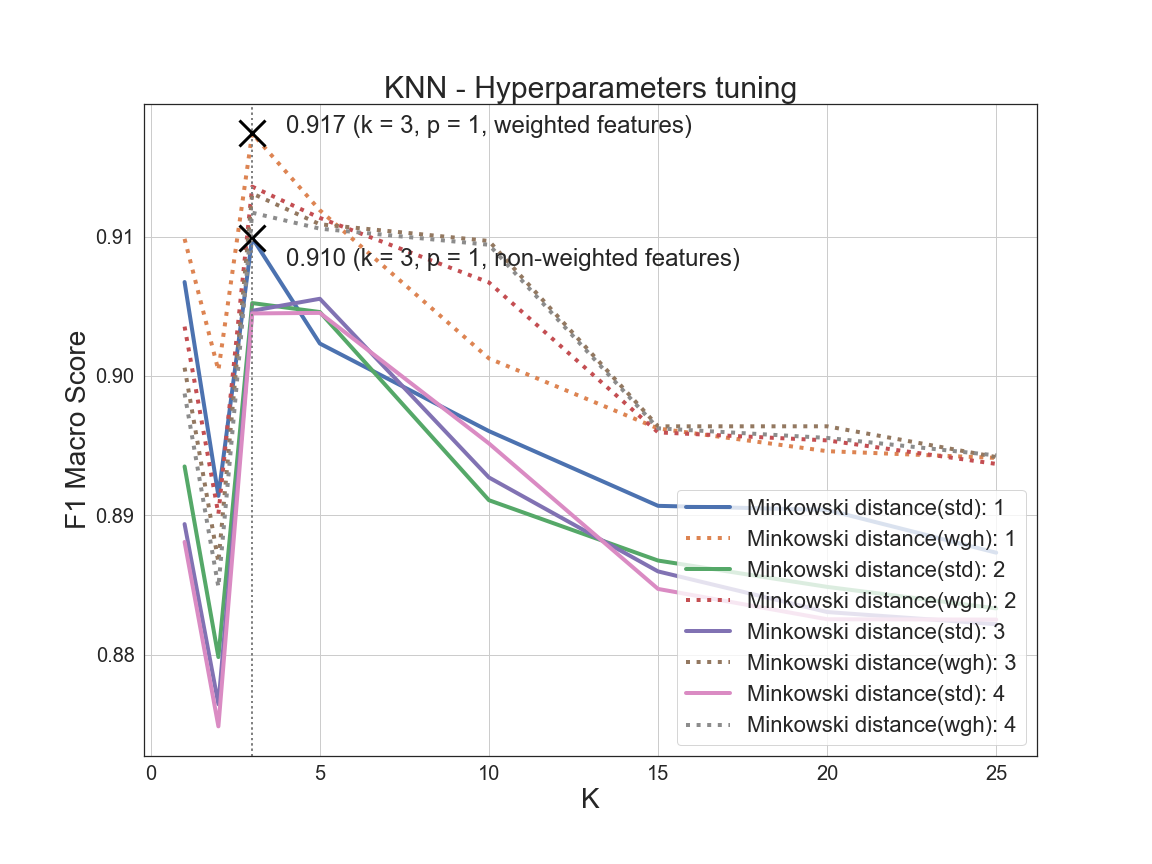
\includegraphics[width=\columnwidth]{chapter5/figure/knn_tuning.png}
	\caption{Hyperparameters p, k tuning, with different weightings}
	\label{fig:knn_tuning}
\end{figure}
The different colours represent the Minkowski distances tested, as well as the different line styles, dotted and continue, represent the weighted and the non-weighted solutions, respectively.

As visible in the picture, the best score, in the usual 10-fold crossvalidation, has been obtained with 5 neighbours, the Manhattan distance, and the weighted solution, which is averagely better than the other one.

The final model has been created with the following call: \textit{KNeighborsClassifier(p=1, n\_neighbors=5)} and it has been fitted with the weighted data, obtaining the following scores in 10-fold-crossvalidation:

\begin{itemize}
	\item[\PencilRight] \textit{Precision}: \textbf{0.924}
	\item[\PencilRight] \textit{Recall}: \textbf{0.917}
	\item[\PencilRight] \textit{F1 score}: \textbf{0.918}
\end{itemize}


\subsection{Text-based Naive Bayes classifier}
In chapter \ref{capitolo4} we created some useful features that helped the above-mentioned classifiers . Anyway we didn't consider enough the tweet texts. A first idea consisted in add a feature that describe the context of the tweets. This task was easily viable using \textit{Google Cloud Natural Language}. Unfortunately, this service only provides a few free calls, and we would not be able to tag all the tweets in our dataset. Moreover, the Context Classification is very specific, and we would have risked to have a too large domain of values. We tried to classify some tweets and we noticed that it was not possible with many of them, since they were just exclamations or contextless sentences. We therefore decided to train a proprietary text classifier. This allowed us to classify texts according to our targets, and our final classifier would have been self-sufficient, without external services.
\subsubsection{Dataset}
Since we wanted to classify texts instead of users, we needed to create a specific dataset.
It had to contain a list of tweets and all the related target. We composed it by binding the target of each tweet to the label of its author. This produced some noise; often bots tweet something different from their goal, to seem more humans. We could accept this problem, since most of the tweets are aimed to a goal.
The shape of the dataset is the following:

\begin{center}
	\begin{tabular}{lr}
		category&\# tweets\\
		\hline\hline
		NSFW&196712\\
		news\_spreaders&280300\\
		spam&453719\\
		fake\_followers&41316\\
		genuine&261233\\
		\hline\\\\
	\end{tabular}
\end{center}

It seems unbalanced, anyway it is appropriate to keep all the data. Some spambot's tweets just contain links and they will be removed in the next steps. Differently, Fake-followers usually don't tweet, or they never tweeted.

\subsubsection{Model}
In order to classify texts, we decided to use a Naive Bayes approach. This algorithm consists in a probabilistic classifier based on the Bayes' theorem. ``Numerous researchers proved that it is effective enough to classify the text in many domains \cite{svm}. Naive Bayes models allow each attribute to contribute towards the final decision equally and independently from other attributes`` \cite{nb}.

Tweets can't be processed as they are. Since this model aims to classify texts basing on its words, we had to clean the dataset from all those parts of the text that are not real or useful words. For example articles, smiles, punctuation should not be taken into consideration. Moreover it is fundamental to reduce inflected words to their word stem. Finally, we need to clean all those noisy parts of the tweets, which is important to allow the final text classifier to consider only real words, in order to identify the context.

Tweets without this pre-processing step look like this:\\

\framebox[\textwidth][l]{\parbox{\textwidth}{\textit{'RT @SteveSchmidtSES: TRUMP disgraced the Presidency and the\\United States at the G-7 summit. From his slovenly appearance to his\\unprepared... https://t.co/KiT29FvJw5'}}}\\

In order to perform this tasks, we used a \textit{sklearn Pipeline}. It is a method that allows to build a custom predictive algorithm. In our case, it contains intermediate steps of data transformation and finally the machine learning algorithm. It works like a generic model, but it perform all the included transformations before processing a data, both in training and prediction steps.

We added to the pipeline the following operations:

\begin{itemize}
	\item[\PencilRight] \textbf{Remove retweet information:}\\
	Delete the texual pattern which indicates that the current status is a retweet. It consists in a "RT @original\_author:". 
	\item[\PencilRight] \textbf{Remove punctuation:}\\
	With regular expressions we removed everythink different from characters and numbers. In this step also smiles and other symbols are removed.
	\item[\PencilRight] \textbf{Remove stopwords:}\\
	stopwords are the most common words that are always used in a language and that can not help to classify a context. Some example of words belonging to this category are articles or prepositions.
	We removed them, by using a stopwords dictionary of \textit{NLTK} libraries.
	\item[\PencilRight] \textbf{Transform uppercase characters into lowercase:}\\
	Before tokenize words, we transformed every character into lowercase, in order to be sure that every word is considered only in one form.
	\item[\PencilRight] \textbf{Apply stemming:}\\
	This is the step where words are reduce to their word stem. Since the text classifier is based on the occurrences of words in the texts, we don't need a correct grammar in our tweets. Instead, words at their basic form are more useful for the target.
	In order to perform this transformation we used \textit{SnowballStemmer} from \textit{NLTK} libraries.
	\item[\PencilRight] \textbf{Apply TF-IDF encoding:}\\
	Finally we applied to each word a TF-IDF encoding. Since we had a huge amount of tweets, without this step we would have risked to give too much importance to the overused wordsand almost nothing importance to the others. Moreover, without using TF-IDF we had a worse performance.
	\item[\PencilRight] \textbf{MultinomialNB:}\\
	This is the final classification algorithm. Thanks to the pipeline it always receives cleaned data, performing a better training and predictions.
	We selected a Naive Bayes classifier for multinomial models since we are dealing with a multi-class problem.
\end{itemize}

\subsubsection{Holdout evaluation}
The final text classifier has the following performance:
\begin{itemize}
	\item[\PencilRight] \textit{F1 score:} \textbf{0.71} with TF-IDF
	\item[\PencilRight] \textit{F1 score:} \textbf{0.64} without TF-IDF
\end{itemize}

Since the other models classify users and not single tweets, we could not use a classifier for texts only.
In order to get a prediction on users, based only on their tweets, the final classification script compute the resulted probabilities for each tweet. Then, for each user, the final prediction consists in the mean of the predictions over his tweets.
% !TEX root = ../thesis.tex
\chapter{Bot classifiers}
\label{capitolo5}
\thispagestyle{empty}

In this chapter we will show the choices and stages behind the final model.
Starting from baseline models, we enhanced the chosen classifiers with handcrafted features coming from the last chapter.\\
We saw and studied the performance improvements with validation approaches, and this phase led us to our current solution.

The result involves three models:
\begin{itemize}
	\item[\PencilRight] a first Random Forest classifier that has been used to provide an early filter on the separation between genuine accounts and bots
	\item[\PencilRight] a second Random Forest that gives a classification among the four studied categories of bots only
	\item[\PencilRight] a Naive Bayes classifier, used over the same classes of the second Random Forest, but which reads and labels the users, according on their tweets only
	\item[\PencilRight] a K-Nearest Neighbours classifier, used over the four bot classes, based on the user features only
\end{itemize}
The algorithms were used together into a pipeline work-flow, whose first step is the detection of bots from humans, thanks to the first binary Random Forest.
Then, the percentage of membership in the bot category is further split into four sub-percentages, which represent the prediction over the inner bot categories.
This last partition is performed by a stacking ensemble, whose goal is to combine the predictions of the three multi-class models.


\section{Baselines}
The choices explained in this section were made at the same time of the ones listed in the Baseline section of the last chapter.

This is, basically, the same stage of the above-mentioned, but in a model-driven perspective.
The features involved are the ones described in section \ref{baseline}, but we started from that base, to try different classifiers over it.
We chose to evaluate the performances of raw classifiers, for both the binary and the multi-class problem.
Each type of classifiers has been tested with the respective dataset, but considering only the baseline features of those data.

Furthermore, no parameters tuning has been applied, in order to minimize the results of our baselines classifier, with their standard settings.
\subsection{Random Forest}
Random forest is an ensemble learning method used in classification tasks and prediction ones as well.

The algorithm builds several \textit{decision trees} and the resulting output is provided by the mode of the predictions coming from the estimators in the forest.

Each decision tree is trained on a subset of the original data, formed by sampling with replacements the whole training set. They share the same splitting criterion, in order to build subtrees, which is the entropy:\\
Every tree computes the Information Gain of each feature, which is the difference, in terms of entropy, between the information gained on the data \textit{D}, before splitting on the attribute \textit{X}, and the one gained after the split, which provides \textit{n} subsets of \textit{D}.
\[{ \mathit{InformationGain(X)} = \mathit{Information(D)} - \mathit{Information_{X}(D)}}\]
where
\[{ \mathit{Information(D)} = - p_{1}\log p_{1} - ... - p_{n} \log p_{n}}\]
and
\[{ \mathit{Information_{X}(D)} = \frac{|D_{1}|}{|D|}Information(D_{1}) + ... + \frac{|D_{n}|}{|D|}Information(D_{n}) }\]
The attribute providing the highest InformationGain, against the others at the same level of the tree, is chosen to perform a split.

The feature set considered by each tree is a random subset of the original pool.

Due to its ability to face overfitting and to the feature importance ranking that it can provide, this tool is often preferred over other models belonging to the same category.

The advantage of preventing overfitting usually comes with a slower prediction time, because it needs enough estimators for this task.
But, for our purpose, there were enough estimators to face the variance problem without affecting the generalization speed.
\subsection{Logistic Regression}
Logistic regression is a common statistical model, that uses a sigmoid function to map the output of a linear regression on a normalized score, giving the probability, for each sample, to belong to the positive class, given its features and a weighting vector:
\[{\displaystyle P(\hat{y}_{i} = +1 | \vec{x}_{i}, \vec{w})={\frac {1}{1+e^{-\vec{w}h(\vec{x}_{i})}}}}\]

Where $ \hat{y}_{i} $ is the predicted target, over the  \textit{$i_{th}$} sample, \textit{$ \vec{x}_{i} $} is the feature vector of that sample, \textit{$ \vec{w} $} represents the weighting vector that has to be learned and \textit{h} is the activation function of the linear regression.

Logistic Regression searches for the weighting vector that matches the highest likelihood and, in order to do that, it minimizes a cross-entropy
error function, provided by the negative log of the likelihood:
\[{ \mathbf{L}(\vec{w}) = -\ln \prod\limits_{i=1}^{n} P(\hat{y}_{i} = +1 | \vec{x}_{i}, \vec{w})}\]

In multi-classes tasks, there are two possible approaches to face the problem:
\begin{itemize}
	\item[\PencilRight] a more general \textit{softmax} function to replace the logistic sigmoid, which assigns the probability, for the  \textit{$i_{th}$} sample, to belong to the class \textit{C}:
	\[{\displaystyle P(\mathbf{C}_{i} | \vec{x}_{i}, \vec{w})={\frac {e^{-\vec{w}h(\vec{x}_{i})}}{\sum\limits_{j = 1}^{n}e^{-\vec{w}h(\vec{x}_{j})}}}}\]
	\item[\PencilRight] ``One-vs-Rest`` method, which for each class builds a model that predicts the target class against all the others.
\end{itemize}
We decided to stick with the default settings of the libraries involved, so OvR was the approach used for the baseline.

\subsection{K-Nearest Neighbors}
K-Nearest Neighbors is an instance-based model used for classification, regression and pattern recognition. It is considered as a lazy learning algorithm, because all the computation is deferred until the prediction phase.
When it performs a classification over a new point, it looks for the \textit{K} nearest samples in the training set, according to a chosen metric, and it assigns, to the unseen sample, the mode of the targets of the retrieved neighbors.

The choices to make are the ones regarding the number \textit{K} of neighbors to consider, the weights to assign to them and the metric to calculate the distance with.
We used the default settings for the metric (\textit{Euclidean distance}) and for the weighting technique (\textit{uniform}), but we chose to consider 10 neighbors, because the automatic setting was \textit{K} = 5, which is the number of our possible targets.
We chose a \textit{K} that is large enough to make the model not too sensible to outliers, and restricted enough to sharpen the classes boundaries.

We first normalized the training data and then we fitted the algorithm on them, in order to simplify the distance computations.

\subsection{Support Vector Machine}
Support Vector Machine is a smart way to do instance-based learning. It can be seen as a generalization of the weighted KNN algorithm, with an arbitrary and feasible \textit{kernel function}, instead of the more generic dot product.

It can be summarised with a support vector $ \mathbf{\vec{x}} $ (a subset of the training set), a weighting vector $ \mathbf{\vec{w}} $ for them and a \textbf{kernel} \textit{K(x, x')} (a similarity function).

In order to make it work properly, three choices must be made:
\begin{itemize}
	\item[\PencilRight] a proper kernel, which is often selected according to experience and domain knowledge of the problem. We wanted to make things simple in this stage, so we used the default kernel function, which is the Radial Basis Function:\label{rbf}
	\[ K(x, x') = exp(- \frac{||x-x'||^{2}}{2\sigma^{2}}) \]
	with $ \sigma $ as a free parameter
	\item[\PencilRight] the weights $ \vec{w} $, which are obtained by maximizing the margin that splits the records belonging to different classes. Each samples are mapped into a space, thanks to what is known as the \textit{kernel trick}. The ``trick`` helps a linear classifier to work on a non-linear problem, applying the kernel function in the prediction phase.\\This process highlights the boundary that separates the points belonging to different classes.
	SVM aims to draw the boundary for the classes, in order to maximize the ``margin`` formed between the closest points that have different targets
	\item[\PencilRight] the support vector $ \vec{x} $, which comes as a consequence of choosing weights
\end{itemize}
Since we were still facing a multitarget problem, the binary nature of SVM must had been adapted to our needs. We decided, once again, to stick with the default setting for non-binary classifications, in order to have only raw baselines to compare.

The multi-target classification is handled with ``One-vs-One`` approach.
It considers all possible pairwise binary classifiers and so it leads to $\frac{N(N-1)}{2}$ individual binary classifiers, where N is the number of the classes in the problem.

In comparison with "One-vs-Rest" approach, ``One-vs-One`` is less sensitive to an imbalanced dataset, but it's more computationally expensive then the the other, which only builds N binary classifiers.
Despite our choices over methods and parameters weren't accurate in this stage as they were in the other ones, we decided to stick with this setting for SVM, because otherwise it would have led us to an irrelevant algorithm, in comparison with the above-mentioned.

\subsection{Comparison and baseline selection}
Different tasks imply different evaluation metrics. Every classifier was validated and selected according to certain indices of goodness. In particular, we followed a triple of metrics that involves Precision, Recall and F1, for the multi-class problem and we aimed to maximize AUC score for the binary case.
\subsubsection{Multi-class metric}
The selected baseline models were tested with a holdout approach at first, then with a crossvalidation method.
We built a Confusion Matrix for each model, in order to bring out goodness indices for each class, such as \textit{True Positive} (TP), \textit{False Positive} (FP) and \textit{False Negative} (FN).
The evaluation metrics considered are \textit{Precision}, \textit{Recall} and \textit{F1 score} and they work on the mentioned indices.
\begin{itemize}
	\item[\PencilRight] $ Precision = \frac{TP}{TP+FP} $\\
	It measures the proportion of positive identifications, for a given target, that was actually correct.
	\item[\PencilRight] $ Recall = \frac{TP}{TP+FN} $\\
	It measures the proportion of actual positive classifications that was identified correctly.
	\item[\PencilRight] $ F1 score = \frac{2(Precision \times Recall )}{Precision+Recall} $\\
	It calculates the harmonic mean of the previous metrics.
\end{itemize}
Every metric is adapted to fit a multi-class problem. For each class, it has been computed this set of measures, and then they were averaged without weights (macro average), in order to not take label imbalance into account.

\subsubsection{Binary metric}
Since this classifier was built for a different purpose, with respect to the multi-class models, the \textit{Area Under the Curve} score (AUC) is the metric we followed, both for baselines and the final model evaluation.
Area Under the Curve represents the goodness of a classifier, in terms of the integral of the \textit{Receiver Operating Characteristic} (ROC curve), defined over the variation of a decision treshold.

The ROC curve lies in a bi-dimensional space, which has the \textit{True Positive Ratio} ($ TPR =  \frac{TP}{TP+FN}$) on the Y-axis, and the False Positive Ratio ($ FPR =  \frac{FP}{FP+TN}$ ) on the X-axis.
In general, a classifier should accomplish more than 0.5 in AUC score, because that threshold represents a random guesser, which has the 50\% of probabilities to detect the actual class.
The more the AUC score tends to 1, the better is the ability of the classifier to distinguish among classes.

The motivation behind the adding of this new metric is that we had a balanced binary dataset, and this metric is a good fit for this kind of problem. Moreover, Botometer claims to have accomplished an AUC of 0.95, on a 10-fold crossvalidation test.
We wanted to get close to that score, using our crafted features.


\subsection{Holdout evaluation}
The holdout evaluation is performed separating the samples in the dataset into training and test subsets. The splitting process is randomized and it requires a bigger portion of the original dataset to be inserted in the training data, comparing to the amount of samples that will form the test set. A common choice is to use a third of the data to evaluate the model.

\subsection{Multi-class}
In this case, we decided to use 75\% of the data for the training set and 25\% for the test set. This choice is a little bit different from the most common one, which builds the training set with 2/3 of the whole data, because we didn't dispose of a huge amount of records, so we preferred this ratio and then trying an other validation method for comparison.
Here we list the algorithms and their parameters, as they were written according to the Scikit-learn library for Python, their confusion matrix and their scores:
\begin{itemize}
	\item[\PencilRight] \textit{RandomForestClassifier(n\_estimators = 10, criterion = 'entropy')}\\
	Confusion matrix:
	
	{
		\centering
		\begin{tabular}{@{}cc|cccc@{}}
			\multicolumn{1}{c}{} &\multicolumn{1}{c}{} &\multicolumn{4}{c}{Predicted class} \\ 
			\multicolumn{1}{c}{} & 
			\multicolumn{1}{c|}{} & 
			\multicolumn{1}{c}{NSFW} & 
			\multicolumn{1}{c}{NS} &
			\multicolumn{1}{c}{SB} & 
			\multicolumn{1}{c}{FF} \\
			\cline{2-6}
			\multirow[c]{4}{*}{\rotatebox[origin=tr]{90}{Actual class}}
			& NSFW  & 1690 & 27 & 12 & 6\\
			& NS  & 27  & 785 & 30 &  0\\
			& SB  & 14  & 39 & 1280 & 5\\
			& FF  & 12 &  7 &  18 & 1215\\
			\cline{2-6}\\
		\end{tabular}\\
	}
	
	Precision: 0.957\\
	Recall: 0.958\\
	F1 score: 0.957

	\item[\PencilRight] \textit{LogisticRegression(fit\_intercept=True, max\_iter=100, penalty='l2')}\\
	Confusion matrix:
	
	{
		\centering
		\begin{tabular}{@{}cc|cccc@{}}
			\multicolumn{1}{c}{} &\multicolumn{1}{c}{} &\multicolumn{4}{c}{Predicted class} \\ 
			\multicolumn{1}{c}{} & 
			\multicolumn{1}{c|}{} & 
			\multicolumn{1}{c}{NSFW} & 
			\multicolumn{1}{c}{NS} &
			\multicolumn{1}{c}{SB} & 
			\multicolumn{1}{c}{FF} \\
			\cline{2-6}
			\multirow[c]{4}{*}{\rotatebox[origin=tr]{90}{Actual class}}
			& NSFW  & 1274 & 213 & 197 & 51\\
			& NS  & 24 & 740 & 75 & 3\\
			& SB  & 29 & 87 & 1144 & 78\\
			& FF  & 204 &  49 &  46 & 953\\
			\cline{2-6}\\
		\end{tabular}\\
	}
	
	Precision: 0.793\\
	Recall: 0.807\\
	F1 score: 0.794
	
	\item[\PencilRight] \textit{KNeighborsClassifier(n\_neighbors=10)}\\
	Confusion matrix:
	
	{
		\centering
		\begin{tabular}{@{}cc|cccc@{}}
			\multicolumn{1}{c}{} &\multicolumn{1}{c}{} &\multicolumn{4}{c}{Predicted class} \\ 
			\multicolumn{1}{c}{} & 
			\multicolumn{1}{c|}{} & 
			\multicolumn{1}{c}{NSFW} & 
			\multicolumn{1}{c}{NS} &
			\multicolumn{1}{c}{SB} & 
			\multicolumn{1}{c}{FF} \\
			\cline{2-6}
			\multirow[c]{4}{*}{\rotatebox[origin=tr]{90}{Actual class}}
			& NSFW  & 1578 & 36 & 60 & 61\\
			& NS  & 81 & 685 & 63 & 13\\
			& SB  & 81 & 32 & 1187 & 38\\
			& FF  & 104 & 6 & 55 & 1087\\
			\cline{2-6}\\
		\end{tabular}\\
	}
	
	Precision: 0.883\\
	Recall: 0.869\\
	F1 score: 0.875
	
	\item[\PencilRight] \textit{SVC(kernel='rbf', decision\_function\_shape='ovo')}\\
	Confusion matrix:
	
	{
		\centering
		\begin{tabular}{@{}cc|ccc@{}}
			\multicolumn{1}{c}{} &\multicolumn{1}{c}{} &\multicolumn{3}{c}{Predicted class} \\ 
			\multicolumn{1}{c}{} & 
			\multicolumn{1}{c|}{} & 
			\multicolumn{1}{c}{NSFW} & 
			\multicolumn{1}{c}{SB} & 
			\multicolumn{1}{c}{FF} \\
			\cline{2-5}
			\multirow[c]{3}{*}{\rotatebox[origin=tr]{90}{Actual class}}
			& NSFW  & 1735 & 0 & 0\\
			& NS  & 842 & 0 & 0\\
			& SB  & 1114 & 223 & 1\\
			& FF  & 483 & 0 & 769\\
			\cline{2-5}\\
		\end{tabular}\\
	}
	
	Precision: 0.603\\
	Recall: 0.445\\
	F1 score: 0.408
	
\end{itemize}

From these evaluations it is possible to see how the Random Forest algorithm outperforms Logistic Regression and Support Vector Machine. This difference colud be driven by the multi-class task. Logistic Regression and SVM need to be adapted to this purpose. Another factor that can discriminate the performances is the choices of the features and their magnitude. Random Forest doesn't require attribute normalization to top its scores, additionally, every feature has been ranked and tested with the inner feature ranking provided by the algorithm. It is possible that some of these attributes need further processing to better support the other models tested.


\subsubsection{Binary}
This evaluation was made with the common splitting ration between train and test set. Since we had 31,212 samples available, well balanced, we used two thirds (20,808) for the training set and the remaining (10,404) for the test set.
We wanted a first term of comparison, so, in the beginning, we evaluated the AUC metric with the holdout technique.
\begin{itemize}
	\item[\PencilRight] \textit{RandomForestClassifier(n\_estimators = 10, criterion = 'entropy')}\\
	Confusion matrix:
	
	{
		\centering
		\begin{tabular}{@{}cc|cc@{}}
			\multicolumn{1}{c}{} &\multicolumn{1}{c}{} &\multicolumn{2}{c}{Predicted class} \\ 
			\multicolumn{1}{c}{} & 
			\multicolumn{1}{c|}{} & 
			\multicolumn{1}{c}{BOT} & 
			\multicolumn{1}{c}{GEN}  \\
			\cline{2-4}
			\multirow[c]{2}{*}{Actual class}
			& BOT  & 4314 & 336\\
			& GEN  & 554 & 4160\\
			\cline{2-4}
			\multicolumn{2}{r|}{AUC} & 
			\multicolumn{2}{l}{0.905}\\
		\end{tabular}\\
	}

	\item[\PencilRight] \textit{LogisticRegression(fit\_intercept=True, max\_iter=100, penalty='l2')}\\
	Confusion matrix:
	
	{
		\centering
		\begin{tabular}{@{}cc|cc@{}}
			\multicolumn{1}{c}{} &\multicolumn{1}{c}{} &\multicolumn{2}{c}{Predicted class} \\ 
			\multicolumn{1}{c}{} & 
			\multicolumn{1}{c|}{} & 
			\multicolumn{1}{c}{BOT} & 
			\multicolumn{1}{c}{GEN}  \\
			\cline{2-4}
			\multirow[c]{2}{*}{Actual class}
			& BOT  & 3124 & 1526\\
			& GEN  & 558 & 4156\\
			\cline{2-4}
			\multicolumn{2}{r|}{AUC} & 
			\multicolumn{2}{l}{0.776}\\
		\end{tabular}\\
	}

	
	\item[\PencilRight] \textit{KNeighborsClassifier(n\_neighbors=10)}\\
	Confusion matrix:
	
	{
		\centering
		\begin{tabular}{@{}cc|cc@{}}
			\multicolumn{1}{c}{} &\multicolumn{1}{c}{} &\multicolumn{2}{c}{Predicted class} \\ 
			\multicolumn{1}{c}{} & 
			\multicolumn{1}{c|}{} & 
			\multicolumn{1}{c}{BOT} & 
			\multicolumn{1}{c}{GEN}  \\
			\cline{2-4}
			\multirow[c]{2}{*}{Actual class}
			& BOT  & 3698 &  952\\
			& GEN  & 1129 & 3585\\
			\cline{2-4}
			\multicolumn{2}{r|}{AUC} & 
			\multicolumn{2}{l}{0.777}\\
		\end{tabular}\\
	}

	
	\item[\PencilRight] \textit{SVC(kernel='rbf')}\\
	Confusion matrix:
	
	{
		\centering
		\begin{tabular}{@{}cc|cc@{}}
			\multicolumn{1}{c}{} &\multicolumn{1}{c}{} &\multicolumn{2}{c}{Predicted class} \\ 
			\multicolumn{1}{c}{} & 
			\multicolumn{1}{c|}{} & 
			\multicolumn{1}{c}{BOT} & 
			\multicolumn{1}{c}{GEN}  \\
			\cline{2-4}
			\multirow[c]{2}{*}{Actual class}
			& BOT  & 4625 & 25\\
			& GEN  & 4676 & 38\\
			\cline{2-4}
			\multicolumn{2}{r|}{AUC} & 
			\multicolumn{2}{l}{0.501}\\
		\end{tabular}\\
	}

\end{itemize}

Once again, Random Forest has the best scores, even in the binary problem. Although, e can see a worsening in the KNN performances in this test. It can be imputable to an ``unlucky`` holdout set or to the fixed parameters tested.

\subsection{Crossvalidation}
This approach is based on repeated holdouts. It is performed by splitting the whole data in \textit{K} non-overlapping folds, leading to \textit{K} different holdout evaluations. The results for each step are stored and the final evaluation is given by the mean of the \textit{K} evaluations. For each evaluation, one fold is used for testing, the other ones for training the models. A common practice is to set \textit{K = 10} and thus averaging 10 different evaluations.
This method is also known as \textit{K-fold crossvalidation}. We used a stratified approach, which takes care about keeping the labels balanced on each fold.

Due the need of performing ten steps, it is computationally more expensive then a simple holdout validation. In our case, it was feasible, in term of speed, because of the models complexity and the data amount. This situation held for both the binary and the mutliclass tasks.

The obtained scores are also more meaningful, with regards to holdout, because they are less sensitive to ``lucky`` or ``unlucky`` splits.

Here is the results for every baseline model:
\subsubsection{Multi-class}
\begin{itemize}
	\item[\PencilRight] \textit{RandomForestClassifier(n\_estimators = 10, criterion = 'entropy')}\\
	Mean precision: 0.947\\
	Mean recall: 0.945\\
	Mean f1 score: 0.943
	\item[\PencilRight]\textit{LogisticRegression(fit\_intercept=True, max\_iter=100, penalty='l2')}\\
	Mean precision: 0.827\\
	Mean recall: 0.815\\
	Mean f1 score: 0.815
	\item[\PencilRight]\textit{KNeighborsClassifier(n\_neighbors=10)}\\
	Mean precision: 0.878\\
	Mean recall: 0.858\\
	Mean f1 score: 0.862
	\item[\PencilRight]\textit{SVC(kernel='rbf', decision\_function\_shape='ovo')}\\
	Mean precision: 0.573\\
	Mean recall: 0.456\\
	Mean f1 score: 0.413
\end{itemize}

As the results show, the Random Forest algorithm is the one that achieves the best performances, even with default settings, on both holdout and 10-fold crossvalidation. We thus decided to consider it as the main tool to build our bot categories classifier. 
\subsubsection{Binary}
\begin{itemize}
	\item[\PencilRight] \textit{RandomForestClassifier(n\_estimators = 10, criterion = 'entropy')}\\
	Mean AUC: 0.916\\
	\item[\PencilRight]\textit{LogisticRegression(fit\_intercept=True, max\_iter=100, penalty='l2')}\\
	Mean AUC: 0.792\\
	\item[\PencilRight]\textit{KNeighborsClassifier(n\_neighbors=10)}\\
	Mean AUC: 0.835\\
	Mean precision: 0.779\\
	\item[\PencilRight]\textit{SVC(kernel='rbf')}\\
	Mean AUC: 0.583\\
\end{itemize}
Even in the binary cases, the Random Forest had the best performance, and it could be imputed to the similar features involved in both problems. Moreover, we could see that the Support Vector Machine emerged as a lightly improved random guesser.


\section{Binary Classifier}
Since our dataset was pretty balanced and we couldn't retrieve many more genuine accounts, we didn't want our instrument to treat this category of users just as one the other bot kinds. It was important to perform a previous filter that was able to give importance to the separation between bots and genuine accounts.

We were inspired by the work made with Botometer \cite{Botometer}, which involved a binary labelled dataset, with bot and genuine accounts.
The researchers built their features, grouped them in six main categories, then they ran a Random Forest algorithm per group.

We already had our feature engineering done, so we decided to test it on this new task.

In order to not to build a poorer version of our multi-class model, we didn't want to use a reduced copy of our dataset, stratifying it by stripping random bots from it. We needed a balanced dataset, with about the same amount of genuines and bots. So, we started from the same dataset used by the Botometer project, in order to have a baseline comparison.
\subsection{Dataset}
The dataset we used for this classification was composed of part of our collected records and of some entries from the Caverlee-2011 dataset, which contains 22,223 content polluters and 19,276 legitimate users, both collected through a social honeypot, as described in their paper \cite{Lee11sevenmonths}.

We used the APIs to retrieve the ids for both genuines and bots, from the Caverlee list. The process provided us 15,687 legitimate user ids, and 15,525 general bot ids (without inner classifications), for a total number of 31,212 samples.
The difference from the original number of entries is due to the age of the dataset. Since 2011, the year of the creation of the list, a lot of accounts have been deleted or suspended.

The feature vector we used is the same that came out from the feature engineering process, except for the specific characterizing features, that weren't considered, because crafted for the inner separation among bots. We excluded the \textit{NSFW\_avg}) image feature, as we noticed it didn't bring much performance boosting with the multi-class models.
The extrinsic features must had been adjusted with new dictionaries, so we had two features: (\textit{bots\_words\_score} and  \textit{genuine\_words\_score}.
Both the features have been computed as for the multi-class case, with up to 1000 non overlapping words in each dictionary.

\subsection{Model}
The model chosen for the purpose was the best performer of the tested baselines: the Random Forest binary classifier.
The algorithm has had its parameters tuned during the validation phase.
We decided to stick with 10-fold crossvalidation, as it was done for the baselines.

After several Grid Search runs, the last round computed had this hyperparameters to combine together:
\begin{itemize}
	\item[\PencilRight] \textit{n\_estimators} = [150, 200, 250, 300, 350, 400, 450, 500]
	\item[\PencilRight]\textit{max\_depth} = [None, 26, 28]
	\item[\PencilRight]\textit{criterion} = 'entropy'
\end{itemize}
\begin{figure}[htp!]
	\centering
	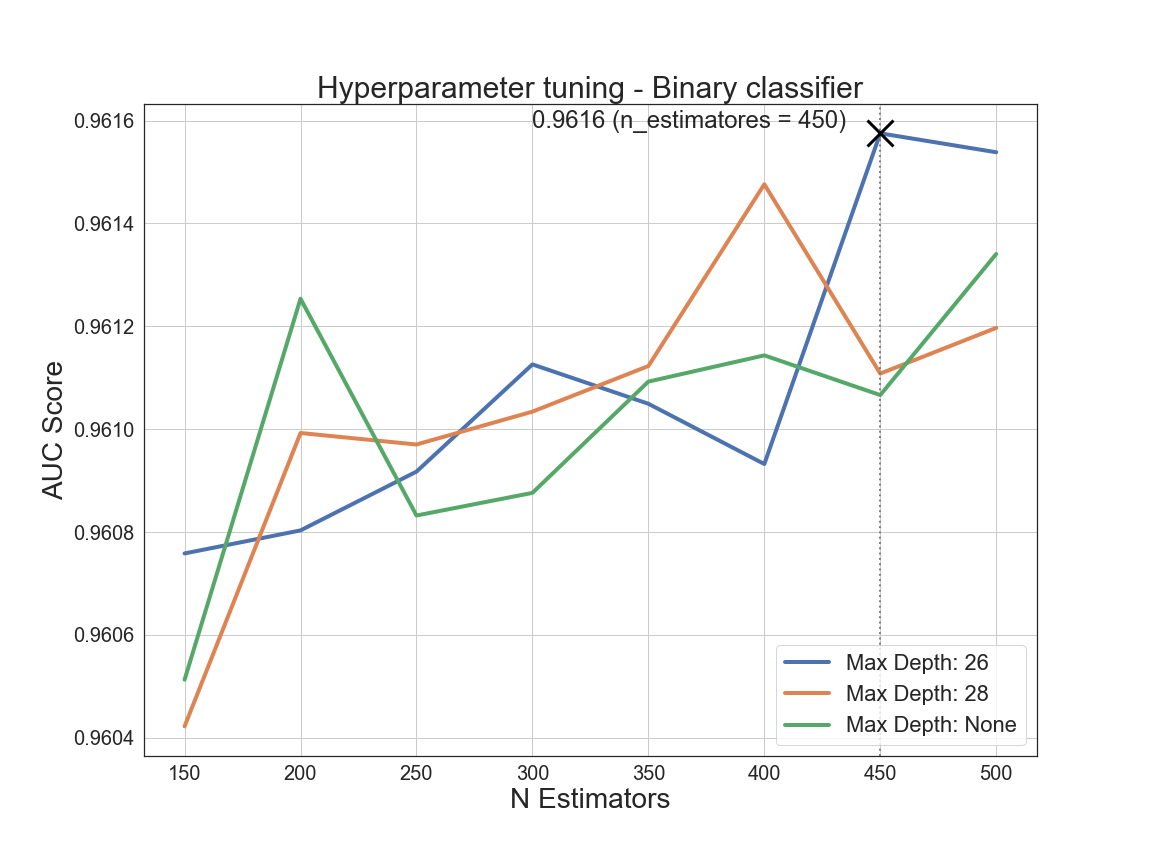
\includegraphics[width=\columnwidth]{chapter5/figure/bon_tuning.png}
	\caption{Grid search results}
	\label{fig:grid_search}
\end{figure}
\begin{figure}[htp!]
	\centering
	\includegraphics[width=\columnwidth]{chapter5/figure/auc.png}
	\caption{ROC curve}
	\label{fig:auc}
\end{figure}
As we can see in Figure \ref{fig:grid_search}, the AUC is increasing with the number of the estimators in the forest. We decided t stop at 450, which corresponds to the highest AUC score, since this phase was aimed to find a comparison term with Botometer, but it didn't represent the final model.
In their paper \cite{Varol}, the Botometer group claims to reach 0.95 in AUC score.

The AUC obtained with our arrangement is equal to 0.96, as shown in Figure \ref{fig:auc}, which is a positive accomplishment, considering that it will be used only as support for the identification of humans among bots, but we didn't crafted specific features as the ones involved in the Botometer project and we didn't have the same amount of data neither.

The model has then been fitted with the hole data, with this settings: \textit{ n\_estimators} = 450, \textit{max\_depth} = 26 and \textit{criterion} = 'entropy'.

\subsection{Validation}

We had an interesting amount of data that were not involved in this task, because of the comparison with the same Botometer's dataset. Since this unseen data had a further discrimination among bots, it was easy to sample some records randomly, replacing their multi-class targets with binary values.
We performed this job to validate the newborn model on unseen and fresher data.
We were interested in testing a model that were trained over ``old`` accounts, with consequent different attributes values and different behaviours on the platform, with younger accounts.

This validations would had given us a preview of the real performance of the model, once it would had been deployed on the internet. The account that a user would test with our application could be younger than the ones included in the Caverlee's list.

We sampled 6,000 accounts, divided in 3,000 genuine and 3,000 bot ids, randomly picked by our multi-class dataset.

The binary model were fitted with its data and it was ready to perform new predictions.

Looking at the most relevant features for the classifier, as shown in Figure \ref{fig:bon_importances}, we could find the \textbf{age} field at the top position.

\begin{figure}[htp!]
	\centering
	\includegraphics[width=\columnwidth]{chapter5/figure/bon_importances.png}
	\caption{Binary Random Forest features ranking}
	\label{fig:bon_importances}
\end{figure}

This was the first warning of a validation performance worsening.
A said before, the age of the accounts in the Caverlee's dataset were higher than the ones in our dataset. In particular, we examined the \textit{age} field of the training set, and the one coming from our validation samples, picked from the mutliclass dataset.
\begin{table}[!htb]
	\caption{Age field comparison among bot accounts}
	\begin{center}
		\begin{tabular}{@{}lr@{}}
			\multicolumn{2}{c}{\textbf{Training Bots}}\\
			\hline\hline
			\multicolumn{2}{c}{\textit{age}}\\
			\hline
			\multicolumn{1}{l}{mean}& \multicolumn{1}{r}{8}\\
			\multicolumn{1}{l}{std}& \multicolumn{1}{r}{0.66}\\
			\multicolumn{1}{l}{min}& \multicolumn{1}{r}{4}\\
			\multicolumn{1}{l}{max}& \multicolumn{1}{r}{12}\\
			\multicolumn{1}{l}{25\%}& \multicolumn{1}{r}{8}\\
			\multicolumn{1}{l}{50\%}& \multicolumn{1}{r}{9}\\
			\multicolumn{1}{l}{75\%}& \multicolumn{1}{r}{9}\\
			\hline\hline
		\end{tabular}
		\begin{tabular}{@{}lr@{}}
			\multicolumn{2}{c}{\textbf{Validation Bots}}\\
			\hline\hline
			\multicolumn{2}{c}{\textit{age}}\\
			\hline
			\multicolumn{1}{l}{mean}& \multicolumn{1}{r}{4.50}\\
			\multicolumn{1}{l}{std}& \multicolumn{1}{r}{2.69}\\
			\multicolumn{1}{l}{min}& \multicolumn{1}{r}{0}\\
			\multicolumn{1}{l}{max}& \multicolumn{1}{r}{11}\\
			\multicolumn{1}{l}{25\%}& \multicolumn{1}{r}{3}\\
			\multicolumn{1}{l}{50\%}& \multicolumn{1}{r}{4}\\
			\multicolumn{1}{l}{75\%}& \multicolumn{1}{r}{6}\\
			\hline\hline
		\end{tabular}
	\end{center}
	\label{table:bots}
\end{table}


\begin{table}[!htb]
	\caption{Age field comparison among genuine accounts}
	\begin{center}
		\begin{tabular}{@{}lr@{}}
			\multicolumn{2}{c}{\textbf{Training Genuine}}\\
			\hline\hline
			\multicolumn{2}{c}{\textit{age}}\\
			\hline
			\multicolumn{1}{l}{mean}& \multicolumn{1}{r}{9.22}\\
			\multicolumn{1}{l}{std}& \multicolumn{1}{r}{0.54}\\
			\multicolumn{1}{l}{min}& \multicolumn{1}{r}{4}\\
			\multicolumn{1}{l}{max}& \multicolumn{1}{r}{12}\\
			\multicolumn{1}{l}{25\%}& \multicolumn{1}{r}{9}\\
			\multicolumn{1}{l}{50\%}& \multicolumn{1}{r}{9}\\
			\multicolumn{1}{l}{75\%}& \multicolumn{1}{r}{9}\\
			\hline\hline
		\end{tabular}
		\begin{tabular}{@{}lr@{}}
			\multicolumn{2}{c}{\textbf{Validation Genuine}}\\
			\hline\hline
			\multicolumn{2}{c}{\textit{age}}\\
			\hline
			\multicolumn{1}{l}{mean}& \multicolumn{1}{r}{6.40}\\
			\multicolumn{1}{l}{std}& \multicolumn{1}{r}{1.94}\\
			\multicolumn{1}{l}{min}& \multicolumn{1}{r}{3}\\
			\multicolumn{1}{l}{max}& \multicolumn{1}{r}{11}\\
			\multicolumn{1}{l}{25\%}& \multicolumn{1}{r}{5}\\
			\multicolumn{1}{l}{50\%}& \multicolumn{1}{r}{6}\\
			\multicolumn{1}{l}{75\%}& \multicolumn{1}{r}{8}\\
			\hline\hline
		\end{tabular}
	\end{center}
	\label{table:genuine}
\end{table}

Like Tables \ref{table:bots} and \ref{table:genuine} show, there is a clear differences in the age attribute, between training and validation set.

We went forward to check if this diversity would had led us to a bad validation performance, or if the model would had handled the predictions in other ways.

The 10-fold crossvalidation on the validation set produced the following confusion matrix, with the correlated AUC score:\\

{
	\centering
	\begin{tabular}{@{}cc|cc@{}}
		\multicolumn{1}{c}{} &\multicolumn{1}{c}{} &\multicolumn{2}{c}{Predicted class} \\ 
		\multicolumn{1}{c}{} & 
		\multicolumn{1}{c|}{} & 
		\multicolumn{1}{c}{BOT} & 
		\multicolumn{1}{c}{GEN}  \\
		\cline{2-4}
		\multirow[c]{2}{*}{Actual class}
		& BOT  & 558 & 2442\\
		& GEN  & 158 & 2842\\
		\cline{2-4}
		\multicolumn{2}{r|}{AUC} & 
		\multicolumn{2}{l}{0.566}\\
		\multicolumn{4}{c}{}\\
	\end{tabular}\\
}
The worsening were real, and it highlighted the short-sighted training phase we performed, trying to top the Botometer performance.

We tried to mitigate this performance loss, by excluding the main suspect from the features set.
Here is the validation performance, without considering the accounts' ages.

{
\centering
\begin{tabular}{@{}cc|cc@{}}
	\multicolumn{1}{c}{} &\multicolumn{1}{c}{} &\multicolumn{2}{c}{Predicted class} \\ 
	\multicolumn{1}{c}{} & 
	\multicolumn{1}{c|}{} & 
	\multicolumn{1}{c}{BOT} & 
	\multicolumn{1}{c}{GEN}  \\
	\cline{2-4}
	\multirow[c]{2}{*}{Actual class}
	& BOT  & 2920 & 20\\
	& GEN  & 1589 & 1411\\
	\cline{2-4}
	\multicolumn{2}{r|}{AUC} & 
	\multicolumn{2}{l}{0.721}\\
	\multicolumn{4}{c}{}\\
\end{tabular}\\
}

The improvement was encouraging, but still not enough to rely on this basic solution.
Considering the bot target as the positive class, we still had too many False Positive in our confusion Matrix. The binary classifier used to tend to identify an user as a bot, with too much confidence. We had to reduce that number, in order to provide a reliable filter in the final prediction pipeline system.

\subsection{Data extension}
The idea we had was to use some data from our multi-class dataset to enrich the binary training set, in order to make the algorithm handle younger and different types of samples from the Twitter population.

In order to perform the extension, we sampled 3,000 genuine accounts and 8,000 bots (2,000 content polluters for each class), all coming from our dataset, and added them to the Caverlee's dataset.
The new training set was composed by 42,212 samples.

We performed a 10-fold-crossvalidation to see the effect of this data refill, sticking to the same hyperparameters found by the last Grid Search. The AUC score measured with these data was 0.963. We could see a slight improvement of the performances, with this data extension. However, we wanted to take a look inside the inner ranking performed by the algorithm, to check if the age field represented an important splitting point.
Figure \ref{fig:bon_importances_ext} shows that the age attribute was still the most considered when the trees had to perform the first splits.

We couldn't blindly follow the AUC score through Grid Searches, without making considerations about what will happen when we will allow people to classify data coming from outside our collected samples.
The age feature would have driven the Random Forest to misclassification over accounts with low \textit{age} values.
Even if the exclusion of that attribute would had made the overall AUC score worse, we had to strip it from the features vector, in order to better generalize on real test cases.

\begin{figure}[htp!]
	\centering
	\includegraphics[width=\columnwidth]{chapter5/figure/bon_importances_extensions.png}
	\caption{Features ranking with augmented data - Top 12 }
	\label{fig:bon_importances_ext}
\end{figure}

While cross-validating the model, we tested the complete features vector (with and without the extension from our dataset) and the one stripped by the age values. The crossvalidation was performed with the same hyperparameters settings of the model fitted with the Caverlee's dataset only.

{
	\centering
	\begin{tabular}{@{}cccc@{}}
		\multicolumn{1}{c}{} & 
		\multicolumn{3}{c}{Fitted data} \\ 
		\cline{2-4}
		\multicolumn{1}{c|}{} & 
		\multicolumn{1}{c|}{original - with \textit{age} } & 
		\multicolumn{1}{c|}{extended - with \textit{age} } & 
		\multicolumn{1}{c|}{extended - without \textit{age}} \\
		\cline{1-4}
		\multicolumn{1}{|c|}{AUC} & 
		\multicolumn{1}{c|}{\textbf{0.961}} & 
		\multicolumn{1}{c|}{\textbf{0.963}} & 
		\multicolumn{1}{c|}{\textbf{0.948}} \\
		\cline{1-4}\\
	\end{tabular}\\
}

The age filed removing made thing worse, but we decided to perform it anyway, because of the good score reached without it, and the flexibility we were giving to the Random Forest. The slight worsening could be also imputed to the biased extrinsic features of that data: those samples came from the multi-class dataset and they originally had the extrinsic features based on the four bot categories' dictionaries.
In order to refill the binary dataset with these new samples, we had to recompute the extrinsic features, applying the analogous method used for the binary purpose.
We didn't recompute the entire dictionaries, we just assigned the scores to the new samples we were introducing, basing the calculations on the already listed words. Those had been exposed in chapter \ref{capitolo4}. This approach aimed to force the algorithm to identify bots and humans, basing its comparisons on the online computations of those features, like in a real-case generalization.

This last configuration was used to performed a further tuning of the parameters.
A new Grid Search brought us the configuration for the hyperparameters shown in Figure \ref{fig:bon_tuning_refil}, leading to the new AUC score, exposed in Figure \ref{fig:bon_refil_auc}.
\begin{figure}[htp!]
	\centering
	\includegraphics[width=\columnwidth]{chapter5/figure/bon_tuning_refill.png}
	\caption{Grid Search with extended data}
	\label{fig:bon_tuning_refil}
\end{figure}
\begin{figure}[htp!]
	\centering
	\includegraphics[width=\columnwidth]{chapter5/figure/refill_auc.png}
	\caption{AUC score with extended data}
	\label{fig:bon_refil_auc}
\end{figure}
The binary classifier has then been fitted with 42,212 samples with 34 features, 600 estimators, entropy splitting criterion and 26 levels of maximum depth.

\section{Multi-class ensemble classifier}
It somehow represents the core of our thesis, it models the starting idea: go deep inside bot identification and search and classify similar behaviours among them.

In this section we will expose the model involved in the multi-class ensemble. In this process, we used a Random Forest algorithm, working on all the crafted features; a KNN model, operating on the user attributes only; a final text-based Naive Bayes classifier, which reads the tweets' texts and classifies them.

At first, this ensemble of these three models should have been blended with the prediction of the binary classifier. That means that the genuine class was part of the labels we were trying to classify, even in the multi-class models. Then, we found an issue in this approach: the binary classifier itself wasn't enough, even including it into the ensemble, to give the right importance to the genuine accounts. This problem emerged because of the others classifiers, as they were trying to classify the genuine class too. They lacked in data with that target, so, basically, they used to treat that category as one other of the bot types.

Even if the results on our validation sets were still good (we accomplished a F1 measure of 0.973), for the final ensemble method, we knew that this method would had yielded to a poor bot vs genuine detection tool. We couldn't accept that situation, because, in order to go deeper than other works, in bot behaviour classifications, we had to provide a solid previous discrimination between humans and automated accounts.

The ensemble method with all the classifiers blended together were replaced with a pipeline, and the multi-class models were trained on bot categories only.
These last classifiers had been put together inside a  ensemble, which returns the final mutliclass probability prediction, based on the opinions of those models, as shown in Figure \ref{fig:stacking_schema}

The different nature of the classifiers, and the feature subsets as well, is one of the strengths of the stacking approach: it combines different opinions about the samples, driven by different classifiers, considering different parameters and attributes; basing on those unlike classifications, it builds its own.

It differs from other ensemble methods as bagging and boosting, because of this miscellaneous schema, and it can be a robust method to exploit the different characteristics of the classifiers stacked together.

\begin{figure}[htp!]
	\centering
	\includegraphics[width=\columnwidth]{chapter5/figure/stacking.png}
	\caption{Multi-class ensemble schema}
	\label{fig:stacking_schema}
\end{figure}
In the following subsections there are the detailed explanations of the three classifier announced before.

\subsection{All-features-based Random Forest classifier}
\subsubsection{Dataset}
During this phase, we used the previously described dataset \ref{sec:dataset} with its four different labels.
The algorithm was fed with 21,445 samples and 37 features. the amount of records were light enough to consider K-fold crossvalidation, without slow the validation down too much.
\subsubsection{Model}
We found ourselves in the situation in which we had some brand new features and we didn't know how useful they were. Obviously, we could appeal to heat-maps or other tools, to highlight the correlations among variables and targets.
However, the model we wanted to develop was the Random Forest, which proved to perform well with F1 score. Since this kind of model exploits its criteria to employ the features, we needed to prove them with a direct approach.

\subsubsection{Features selection}
A useful advantage of the Random Forest algorithm is the ability to provide a feature ranking, according to its splitting criterion.
We retrieved this standing, in order to see if we would have found some of the ones coming out from feature engineering at the top positions.
The algorithm ranking ranked the features this way: 1. \textit{favourites\_count} (0.179), 2. \textit{nsfw\_profile} (0.068), 3. \textit{freq} (0.061), 4. \textit{tweet\_intradistance} (0.060), 5. \textit{news\_spreaders\_words\_score} (0.058), 6. \textit{statuses\_count} (0.053), 7. \textit{avg\_len} (0.051), 8. \textit{followers\_count} (0.051), 9. \textit{NSFW\_words\_score} (0.043), 10. \textit{ret\_perc} (0.041), 11. \textit{min\_len} (0.038), 12. \textit{spam\_bots\_words\_score} (0.035), ...  37. \textit{min\_fav} (0.0001).

\begin{figure}[htp!]
	\centering
	\includegraphics[width=\columnwidth]{chapter5/figure/top_12_features_importances.png}
	\caption{Random Forest top-12 feature ranking}
	\label{fig:feature_rank}
\end{figure}

As Figure \ref{fig:feature_rank} shows, we could find some of our crafted features inside this list: lots of tweets descriptive features (\textit{avg\_len, freq, ret\_perc}, etc...), as well as the \textit{tweet\_intradistance} attribute and three of the four extrinsic features, like \textit{news\_spreaders\_words\_score}, \textit{NSFW\_words\_score} and the \textit{spam\_bots\_words\_score}.
This picture confirmed us that the idea behind those features was useful.

Since those attributes were thought to belong to different clusters, we decided to try several combinations of those feature clusters, validating the model on them with a crossvalidation. The purpose of this stage was to see if some groups of features were enough to describe the real problem, or if some group would shown up as irrelevant.
To face this evaluation, we performed a light-weighted Grid Search, which is a method that takes desired ranges of hyperparameters and tries all the possible permutations of them, looking for the best combination, in terms of a certain metric.

We are talking about a light-weight version of this tool, because we just went through different numbers of tree estimators in the forest. The different feature groups are not considered as hyperparameters and are not handled by the Scikit-learn implementation of the Grid Search.
We had to manage the different training by our own, looking how the test score would have changed along with the increasing number of estimators and the different set of features.

Grid Search uses crossvalidation to find the better estimators for the models, and this approach was right for our situation.
Due to the multi-class nature and some imbalances with the labels, we decided to follow the F1 score metric to asses the value of our model.

The features were organized in clusters, as described in Chapter \ref{capitolo4}.
We had the user features, the descriptive features, the intrinsic features, the extrinsic and the image features. Then we tried the model with the entire set of 38 attributes.
As shown in Figure \ref{fig:feature_clusters}, the best configuration seems to involve the whole set of features, as it reaches these scores, with 100 estimators: \textit{Precision} = 0.978, \textit{Recall} = 0.976, \textbf{\textit{F1}}= 0.977.

\begin{figure}[htp!]
	\centering
	\includegraphics[width=\columnwidth]{chapter5/figure/feature_cluster_f1.png}
	\caption{Performance over different feature clusters}
	\label{fig:feature_clusters}
\end{figure}

The model has been tested with the default value for the maximum depth in the trees, which is set to 'None'. It means that the trees are expanded until every leaf is pure, or all leaves contain one sample.

In order to try all the alternatives, we setted a test involving the performance of the model, when it was working on an increasing number of features.
We had the ranking provided by the forest itself, so we started by testing only the most important attribute, adding one feature at time, until the least important was included.
We were looking for some changing in the scores, that would have pointed to a lighter model, with the exclusion of some features.
Figures \ref{fig:feat_prec}, \ref{fig:feat_rec}, \ref{fig:feat_f1} show the trends of the Precision, the Recall and the F1, respectively, along with the number of features tested.
 \begin{figure}[htp!]
 	\centering
 	\includegraphics[width=\columnwidth]{chapter5/figure/precision_along_features.png}
 	\caption{Precision trend along with number of features tested}
 	\label{fig:feat_prec}
 \end{figure}
\begin{figure}[htp!]
	\centering
	\includegraphics[width=\columnwidth]{chapter5/figure/recall_along_features.png}
	\caption{Recall trend along with number of features tested}
	\label{fig:feat_rec}
\end{figure}
\begin{figure}[htp!]
	\centering
	\includegraphics[width=\columnwidth]{chapter5/figure/f1_along_features.png}
	\caption{F1 trend along with number of features tested}
	\label{fig:feat_f1}
\end{figure}

As all the Figures show, the best solution possible, looking at both the three metrics, is the one involving all the 37 components of the feature vector.
There was the possibility to choose the second result, which wanted only the first 28 features, in terms of importance for the Random Forest. However, we weren't struggling with heavy models or long prediction times and the Random Forest algorithm handles the overfitting problem properly, even with complex models.
Thus, we moved on with the entire feature vector as support for the classification goal.

We then continued with a proper Grid Search over the whole number of features.
\subsubsection{Hyperparameters Tuning}
The algorithms rely on parameters in order to fit a problem.
Once the number of featured was picked, as well as the model, we needed to consider the possible hyperparameter ranges. 
The Grid Search method from Scikit-learn helped us, once again, during this exploration.
Since we were testing a Random Forest, we wanted to play with the number of estimators (tree) to include in the pool, as well as the maximum depth of each tree and the splitting criterion.

\begin{figure}[htp!]
	\centering
	\includegraphics[width=\columnwidth]{chapter5/figure/multiclass_rf_tuning_gini.png}
	\caption{F1 scores with ``Gini`` criterion - close-up view}
	\label{fig:rf_tuning_gini}
\end{figure}
\begin{figure}[htp!]
	\centering
	\includegraphics[width=\columnwidth]{chapter5/figure/multiclass_rf_tuning.png}
	\caption{F1 scores with ``Entropy`` criterion - close-up view}
	\label{fig:rf_tuning_entropy}
\end{figure}

The Figures \ref{fig:rf_tuning_gini}, \ref{fig:rf_tuning_entropy} show how the average F1 score, measured on 10-fold crossvalidation, changes with the increasing of the number of estimators in the forest.
The different coloured lines represent the \textit{max\_depth} hyperparameter.
The first Figure (\ref{fig:rf_tuning_gini}) shows the Grid Search results, with the \textit{gini} splitting criterion.
The second one (\ref{fig:rf_tuning_entropy}) represent the situation having \textit{entropy} as a splitting choice.
We combined nine numbers of estimators (200, 250, 300, 350, 400, 450, 500, 550, 600), together with three different maximum depths for the trees (26, 28, None) and the two above-mentioned splitting criteria.

We could observe a peak, for both criteria, in correspondence with 400 estimators.
Although the Gini-based forest's score didn't seem a bad point, we went with the Information Gain splitting criterion, which si also the same we used to rank the features of our data.

The final configuration involves 400 trees, the Information Gain criterion and the maximum reachable depth (for each of the 400 estimators) equal to 28 levels, yielding the following scores in 10-fold-crossvalidation:
\begin{itemize}
	\item[\PencilRight] \textit{Precision}: \textbf{0.979}
	\item[\PencilRight] \textit{Recall}: \textbf{0.977}
	\item[\PencilRight] \textit{F1 score}: \textbf{0.978}
\end{itemize}

Figure (\ref{fig:tree}) shows an example of one of the estimators of the final model, plotted with Matplotlib library for Python. It has been represented with the first two levels of depth, for visualizations reasons.

\begin{figure}[htp!]
	\centering
	\includegraphics[width=\columnwidth]{chapter5/figure/tree.png}
	\caption{Tree estimator of the Random Forest model}
	\label{fig:tree}
\end{figure}

As the picture shows, this tree used the \textit{tweet\_intradistance} feature as root, in order to perform its first split on that attribute.

The first algorithm of the multi-class ensemble was completed and ready to be combined with the following models.

\subsection{User-based KNN classifier}
The Random Forest model represents somehow the core of the ensemble, as it was trained on the entire feature vector, with all the data we had for the purpose. A massive attention for parameters and features were given for that classifier. 
However, we wanted to put it into an ensemble, not to improve its already strong stability over outliers, but to support it with different perspectives.

We noticed, as shown in the previous Figure \ref{fig:feature_clusters}, that the user features were a good group to build a classifier on. Thus, we started thinking how to implement such support, and we basically looked at our baselines.

The model that had the best performance, not considering the Random Forest, was the K-Nearest Neighbors algorithm.

We didn't want this model to work the entire feature vector, because we knew that it would had been overlooked by the Random Forest. Instead, we wanted it to concentrate on the features that describe the users, without the information driven by their tweets. Therefore, we relied on the user features, with the extension of the image feature that assesses the NSFW score to the profile picture. This extension wa due to the fact that such feature doesn't need the user's tweets to be computed; it can be seen as one of the user features as the others of that group.

We hoped that treating the data before, or during, the training phase, would had brought to a good sustain for the first multi-class model, where needed.

\subsubsection{Dataset}
The dataset is composed of the same number (21,445) of samples of the first multitarget Random Forest, but preserving only the twelve features belonging to the user group, plus the NSFW\_profile attribute coming from the image features group.

\small
\begin{center}
	\begin{tabular}{ll}
		\\Feature vector\\
		\hline\hline
		default\_profile, favourites\_count, followers\_count\\
		friends\_count, listed\_count, screen\_name\_len\\
		statuses\_count, url, description\_len, NSFW\_profile\\
		name\_len, profile\_use\_background\_image, age\\\hline\\
	\end{tabular}
\end{center}
\normalsize

\subsubsection{Model}

This model is quite simple and doesn't require much effort in interpolating several hyperparameters. But this doesn't mean that it is a closed box algorithm. It can be improved by paying attentions to some details. In particular there had been done three considerations, and they were regarding

\begin{itemize}
	\item[\PencilRight]\textbf{Hyperparameters}\\
	The main hyperparameters that can be combined together are the number \textit{k} of neighbours ti consider, when performing a prediction, and the distance metric used by the calculations of the distances.
	The Scikit-learn implementation of the algorithm uses the \textit{Minkowski} metric, which describes the \textbf{L}\textsubscript{p} norm: 
	\[ \mathit{L_{p}} = (\sum\limits_{i = 1}^{n}|x_{i} - y_{i}|^{p})^{1/p} \]
	This metric is a generalization of the \textbf{L}\textsubscript{2} norm, also known as the Euclidean distance.
	The library we used allowed us to tune the \textit{p} hyperparameter, which indicates the metric used: \textit{p} = 1 means L\textsubscript{1} norm, the Manhattan Distance, when \textit{p} = 2 stands for the Euclidean.
	Higher values of \textit{p} are available, with other metric involved.
	
	We tried several values for both \textit{p} and \textit{k}, obtaining different results.
	However, the overall decision had to take in consideration also other two factors, the features weighting and the kernel function.
	
	\item[\PencilRight]\textbf{Features Weighting}\\
	The KNN algorithm aims to map the samples into a space and then it looks for the distances among them. In order to have best mapped space, it is reasonable to perform a weighting over the data. With this approach, the mapping would change and some points could result both as closer or more distant from each others.
	
	We performed some tests on four configurations. The first one didn't involve a weighting vector, while the second one was a standard normalization of the features.
	This last option provided weak results, with the same configurations of parameters, and thus were discarded from further analysis.

	The third option, which was the most interesting, was built by computing the Information Gain for each feature, using the inner ability of the Random Forest classifier, and then by applying the weights on the attributes, basing the coefficients on the scores provided by the ranking.
	This method emerged as the most effective, in the overall score.
	
	The last one was implemented as a Gaussian Kernel, which exploits the above-explained Radial Basis Function \ref{rbf}.
	This attempt fell shorter then the standard normalization, and it could be imputable to an overestimation of the ability to approximate the probability density of our data.
	It seemed that the Gaussian-based weighting wasn't a good fit for the problem.
\end{itemize}

We ran a Grid Search session over an increasing number of neighbours and the first four coefficients of the Minkowski distance.
All the combinations were tested with both the non-weighted data and the Entropy-based weighted data.
The results obtained are highlighted in Figure \ref{fig:knn_tuning}

\begin{figure}
	\includegraphics[width=\columnwidth]{chapter5/figure/knn_tuning.png}
	\caption{Hyperparameters p, k tuning, with different weightings}
	\label{fig:knn_tuning}
\end{figure}
The different colours represent the Minkowski distances tested, as well as the different line styles, dotted and continue, represent the weighted and the non-weighted solutions, respectively.

As visible in the picture, the best score, in the usual 10-fold crossvalidation, has been obtained with 5 neighbours, the Manhattan distance, and the weighted solution, which is averagely better than the other one.

The final model has been created with the following call: \textit{KNeighborsClassifier(p=1, n\_neighbors=5)} and it has been fitted with the weighted data, obtaining the following scores in 10-fold-crossvalidation:

\begin{itemize}
	\item[\PencilRight] \textit{Precision}: \textbf{0.924}
	\item[\PencilRight] \textit{Recall}: \textbf{0.917}
	\item[\PencilRight] \textit{F1 score}: \textbf{0.918}
\end{itemize}


\subsection{Text-based Naive Bayes classifier}
In chapter \ref{capitolo4} we created some useful features that helped the above-mentioned classifiers . Anyway we didn't consider enough the tweet texts. A first idea consisted in add a feature that describe the context of the tweets. This task was easily viable using \textit{Google Cloud Natural Language}. Unfortunately, this service only provides a few free calls, and we would not be able to tag all the tweets in our dataset. Moreover, the Context Classification is very specific, and we would have risked to have a too large domain of values. We tried to classify some tweets and we noticed that it was not possible with many of them, since they were just exclamations or contextless sentences. We therefore decided to train a proprietary text classifier. This allowed us to classify texts according to our targets, and our final classifier would have been self-sufficient, without external services.
\subsubsection{Dataset}
Since we wanted to classify texts instead of users, we needed to create a specific dataset.
It had to contain a list of tweets and all the related target. We composed it by binding the target of each tweet to the label of its author. This produced some noise; often bots tweet something different from their goal, to seem more humans. We could accept this problem, since most of the tweets are aimed to a goal.
The shape of the dataset is the following:

\begin{center}
	\begin{tabular}{lr}
		category&\# tweets\\
		\hline\hline
		NSFW&196712\\
		news\_spreaders&280300\\
		spam&453719\\
		fake\_followers&41316\\
		genuine&261233\\
		\hline\\\\
	\end{tabular}
\end{center}

It seems unbalanced, anyway it is appropriate to keep all the data. Some spambot's tweets just contain links and they will be removed in the next steps. Differently, Fake-followers usually don't tweet, or they never tweeted.

\subsubsection{Model}
In order to classify texts, we decided to use a Naive Bayes approach. This algorithm consists in a probabilistic classifier based on the Bayes' theorem. ``Numerous researchers proved that it is effective enough to classify the text in many domains \cite{svm}. Naive Bayes models allow each attribute to contribute towards the final decision equally and independently from other attributes`` \cite{nb}.

Tweets can't be processed as they are. Since this model aims to classify texts basing on its words, we had to clean the dataset from all those parts of the text that are not real or useful words. For example articles, smiles, punctuation should not be taken into consideration. Moreover it is fundamental to reduce inflected words to their word stem. Finally, we need to clean all those noisy parts of the tweets, which is important to allow the final text classifier to consider only real words, in order to identify the context.

Tweets without this pre-processing step look like this:\\

\framebox[\textwidth][l]{\parbox{\textwidth}{\textit{'RT @SteveSchmidtSES: TRUMP disgraced the Presidency and the\\United States at the G-7 summit. From his slovenly appearance to his\\unprepared... https://t.co/KiT29FvJw5'}}}\\

In order to perform this tasks, we used a \textit{sklearn Pipeline}. It is a method that allows to build a custom predictive algorithm. In our case, it contains intermediate steps of data transformation and finally the machine learning algorithm. It works like a generic model, but it perform all the included transformations before processing a data, both in training and prediction steps.

We added to the pipeline the following operations:

\begin{itemize}
	\item[\PencilRight] \textbf{Remove retweet information:}\\
	Delete the texual pattern which indicates that the current status is a retweet. It consists in a "RT @original\_author:". 
	\item[\PencilRight] \textbf{Remove punctuation:}\\
	With regular expressions we removed everythink different from characters and numbers. In this step also smiles and other symbols are removed.
	\item[\PencilRight] \textbf{Remove stopwords:}\\
	stopwords are the most common words that are always used in a language and that can not help to classify a context. Some example of words belonging to this category are articles or prepositions.
	We removed them, by using a stopwords dictionary of \textit{NLTK} libraries.
	\item[\PencilRight] \textbf{Transform uppercase characters into lowercase:}\\
	Before tokenize words, we transformed every character into lowercase, in order to be sure that every word is considered only in one form.
	\item[\PencilRight] \textbf{Apply stemming:}\\
	This is the step where words are reduce to their word stem. Since the text classifier is based on the occurrences of words in the texts, we don't need a correct grammar in our tweets. Instead, words at their basic form are more useful for the target.
	In order to perform this transformation we used \textit{SnowballStemmer} from \textit{NLTK} libraries.
	\item[\PencilRight] \textbf{Apply TF-IDF encoding:}\\
	Finally we applied to each word a TF-IDF encoding. Since we had a huge amount of tweets, without this step we would have risked to give too much importance to the overused wordsand almost nothing importance to the others. Moreover, without using TF-IDF we had a worse performance.
	\item[\PencilRight] \textbf{MultinomialNB:}\\
	This is the final classification algorithm. Thanks to the pipeline it always receives cleaned data, performing a better training and predictions.
	We selected a Naive Bayes classifier for multinomial models since we are dealing with a multi-class problem.
\end{itemize}

\subsubsection{Holdout evaluation}
The final text classifier has the following performance:
\begin{itemize}
	\item[\PencilRight] \textit{F1 score:} \textbf{0.71} with TF-IDF
	\item[\PencilRight] \textit{F1 score:} \textbf{0.64} without TF-IDF
\end{itemize}

Since the other models classify users and not single tweets, we could not use a classifier for texts only.
In order to get a prediction on users, based only on their tweets, the final classification script compute the resulted probabilities for each tweet. Then, for each user, the final prediction consists in the mean of the predictions over his tweets.
% !TEX root = ../thesis.tex
\chapter{Bot classifiers}
\label{capitolo5}
\thispagestyle{empty}

In this chapter we will show the choices and stages behind the final model.
Starting from baseline models, we enhanced the chosen classifiers with handcrafted features coming from the last chapter.\\
We saw and studied the performance improvements with validation approaches, and this phase led us to our current solution.

The result involves three models:
\begin{itemize}
	\item[\PencilRight] a first Random Forest classifier that has been used to provide an early filter on the separation between genuine accounts and bots
	\item[\PencilRight] a second Random Forest that gives a classification among the four studied categories of bots only
	\item[\PencilRight] a Naive Bayes classifier, used over the same classes of the second Random Forest, but which reads and labels the users, according on their tweets only
	\item[\PencilRight] a K-Nearest Neighbours classifier, used over the four bot classes, based on the user features only
\end{itemize}
The algorithms were used together into a pipeline work-flow, whose first step is the detection of bots from humans, thanks to the first binary Random Forest.
Then, the percentage of membership in the bot category is further split into four sub-percentages, which represent the prediction over the inner bot categories.
This last partition is performed by a stacking ensemble, whose goal is to combine the predictions of the three multi-class models.


\section{Baselines}
The choices explained in this section were made at the same time of the ones listed in the Baseline section of the last chapter.

This is, basically, the same stage of the above-mentioned, but in a model-driven perspective.
The features involved are the ones described in section \ref{baseline}, but we started from that base, to try different classifiers over it.
We chose to evaluate the performances of raw classifiers, for both the binary and the multi-class problem.
Each type of classifiers has been tested with the respective dataset, but considering only the baseline features of those data.

Furthermore, no parameters tuning has been applied, in order to minimize the results of our baselines classifier, with their standard settings.
\subsection{Random Forest}
Random forest is an ensemble learning method used in classification tasks and prediction ones as well.

The algorithm builds several \textit{decision trees} and the resulting output is provided by the mode of the predictions coming from the estimators in the forest.

Each decision tree is trained on a subset of the original data, formed by sampling with replacements the whole training set. They share the same splitting criterion, in order to build subtrees, which is the entropy:\\
Every tree computes the Information Gain of each feature, which is the difference, in terms of entropy, between the information gained on the data \textit{D}, before splitting on the attribute \textit{X}, and the one gained after the split, which provides \textit{n} subsets of \textit{D}.
\[{ \mathit{InformationGain(X)} = \mathit{Information(D)} - \mathit{Information_{X}(D)}}\]
where
\[{ \mathit{Information(D)} = - p_{1}\log p_{1} - ... - p_{n} \log p_{n}}\]
and
\[{ \mathit{Information_{X}(D)} = \frac{|D_{1}|}{|D|}Information(D_{1}) + ... + \frac{|D_{n}|}{|D|}Information(D_{n}) }\]
The attribute providing the highest InformationGain, against the others at the same level of the tree, is chosen to perform a split.

The feature set considered by each tree is a random subset of the original pool.

Due to its ability to face overfitting and to the feature importance ranking that it can provide, this tool is often preferred over other models belonging to the same category.

The advantage of preventing overfitting usually comes with a slower prediction time, because it needs enough estimators for this task.
But, for our purpose, there were enough estimators to face the variance problem without affecting the generalization speed.
\subsection{Logistic Regression}
Logistic regression is a common statistical model, that uses a sigmoid function to map the output of a linear regression on a normalized score, giving the probability, for each sample, to belong to the positive class, given its features and a weighting vector:
\[{\displaystyle P(\hat{y}_{i} = +1 | \vec{x}_{i}, \vec{w})={\frac {1}{1+e^{-\vec{w}h(\vec{x}_{i})}}}}\]

Where $ \hat{y}_{i} $ is the predicted target, over the  \textit{$i_{th}$} sample, \textit{$ \vec{x}_{i} $} is the feature vector of that sample, \textit{$ \vec{w} $} represents the weighting vector that has to be learned and \textit{h} is the activation function of the linear regression.

Logistic Regression searches for the weighting vector that matches the highest likelihood and, in order to do that, it minimizes a cross-entropy
error function, provided by the negative log of the likelihood:
\[{ \mathbf{L}(\vec{w}) = -\ln \prod\limits_{i=1}^{n} P(\hat{y}_{i} = +1 | \vec{x}_{i}, \vec{w})}\]

In multi-classes tasks, there are two possible approaches to face the problem:
\begin{itemize}
	\item[\PencilRight] a more general \textit{softmax} function to replace the logistic sigmoid, which assigns the probability, for the  \textit{$i_{th}$} sample, to belong to the class \textit{C}:
	\[{\displaystyle P(\mathbf{C}_{i} | \vec{x}_{i}, \vec{w})={\frac {e^{-\vec{w}h(\vec{x}_{i})}}{\sum\limits_{j = 1}^{n}e^{-\vec{w}h(\vec{x}_{j})}}}}\]
	\item[\PencilRight] ``One-vs-Rest`` method, which for each class builds a model that predicts the target class against all the others.
\end{itemize}
We decided to stick with the default settings of the libraries involved, so OvR was the approach used for the baseline.

\subsection{K-Nearest Neighbors}
K-Nearest Neighbors is an instance-based model used for classification, regression and pattern recognition. It is considered as a lazy learning algorithm, because all the computation is deferred until the prediction phase.
When it performs a classification over a new point, it looks for the \textit{K} nearest samples in the training set, according to a chosen metric, and it assigns, to the unseen sample, the mode of the targets of the retrieved neighbors.

The choices to make are the ones regarding the number \textit{K} of neighbors to consider, the weights to assign to them and the metric to calculate the distance with.
We used the default settings for the metric (\textit{Euclidean distance}) and for the weighting technique (\textit{uniform}), but we chose to consider 10 neighbors, because the automatic setting was \textit{K} = 5, which is the number of our possible targets.
We chose a \textit{K} that is large enough to make the model not too sensible to outliers, and restricted enough to sharpen the classes boundaries.

We first normalized the training data and then we fitted the algorithm on them, in order to simplify the distance computations.

\subsection{Support Vector Machine}
Support Vector Machine is a smart way to do instance-based learning. It can be seen as a generalization of the weighted KNN algorithm, with an arbitrary and feasible \textit{kernel function}, instead of the more generic dot product.

It can be summarised with a support vector $ \mathbf{\vec{x}} $ (a subset of the training set), a weighting vector $ \mathbf{\vec{w}} $ for them and a \textbf{kernel} \textit{K(x, x')} (a similarity function).

In order to make it work properly, three choices must be made:
\begin{itemize}
	\item[\PencilRight] a proper kernel, which is often selected according to experience and domain knowledge of the problem. We wanted to make things simple in this stage, so we used the default kernel function, which is the Radial Basis Function:\label{rbf}
	\[ K(x, x') = exp(- \frac{||x-x'||^{2}}{2\sigma^{2}}) \]
	with $ \sigma $ as a free parameter
	\item[\PencilRight] the weights $ \vec{w} $, which are obtained by maximizing the margin that splits the records belonging to different classes. Each samples are mapped into a space, thanks to what is known as the \textit{kernel trick}. The ``trick`` helps a linear classifier to work on a non-linear problem, applying the kernel function in the prediction phase.\\This process highlights the boundary that separates the points belonging to different classes.
	SVM aims to draw the boundary for the classes, in order to maximize the ``margin`` formed between the closest points that have different targets
	\item[\PencilRight] the support vector $ \vec{x} $, which comes as a consequence of choosing weights
\end{itemize}
Since we were still facing a multitarget problem, the binary nature of SVM must had been adapted to our needs. We decided, once again, to stick with the default setting for non-binary classifications, in order to have only raw baselines to compare.

The multi-target classification is handled with ``One-vs-One`` approach.
It considers all possible pairwise binary classifiers and so it leads to $\frac{N(N-1)}{2}$ individual binary classifiers, where N is the number of the classes in the problem.

In comparison with "One-vs-Rest" approach, ``One-vs-One`` is less sensitive to an imbalanced dataset, but it's more computationally expensive then the the other, which only builds N binary classifiers.
Despite our choices over methods and parameters weren't accurate in this stage as they were in the other ones, we decided to stick with this setting for SVM, because otherwise it would have led us to an irrelevant algorithm, in comparison with the above-mentioned.

\subsection{Comparison and baseline selection}
Different tasks imply different evaluation metrics. Every classifier was validated and selected according to certain indices of goodness. In particular, we followed a triple of metrics that involves Precision, Recall and F1, for the multi-class problem and we aimed to maximize AUC score for the binary case.
\subsubsection{Multi-class metric}
The selected baseline models were tested with a holdout approach at first, then with a crossvalidation method.
We built a Confusion Matrix for each model, in order to bring out goodness indices for each class, such as \textit{True Positive} (TP), \textit{False Positive} (FP) and \textit{False Negative} (FN).
The evaluation metrics considered are \textit{Precision}, \textit{Recall} and \textit{F1 score} and they work on the mentioned indices.
\begin{itemize}
	\item[\PencilRight] $ Precision = \frac{TP}{TP+FP} $\\
	It measures the proportion of positive identifications, for a given target, that was actually correct.
	\item[\PencilRight] $ Recall = \frac{TP}{TP+FN} $\\
	It measures the proportion of actual positive classifications that was identified correctly.
	\item[\PencilRight] $ F1 score = \frac{2(Precision \times Recall )}{Precision+Recall} $\\
	It calculates the harmonic mean of the previous metrics.
\end{itemize}
Every metric is adapted to fit a multi-class problem. For each class, it has been computed this set of measures, and then they were averaged without weights (macro average), in order to not take label imbalance into account.

\subsubsection{Binary metric}
Since this classifier was built for a different purpose, with respect to the multi-class models, the \textit{Area Under the Curve} score (AUC) is the metric we followed, both for baselines and the final model evaluation.
Area Under the Curve represents the goodness of a classifier, in terms of the integral of the \textit{Receiver Operating Characteristic} (ROC curve), defined over the variation of a decision treshold.

The ROC curve lies in a bi-dimensional space, which has the \textit{True Positive Ratio} ($ TPR =  \frac{TP}{TP+FN}$) on the Y-axis, and the False Positive Ratio ($ FPR =  \frac{FP}{FP+TN}$ ) on the X-axis.
In general, a classifier should accomplish more than 0.5 in AUC score, because that threshold represents a random guesser, which has the 50\% of probabilities to detect the actual class.
The more the AUC score tends to 1, the better is the ability of the classifier to distinguish among classes.

The motivation behind the adding of this new metric is that we had a balanced binary dataset, and this metric is a good fit for this kind of problem. Moreover, Botometer claims to have accomplished an AUC of 0.95, on a 10-fold crossvalidation test.
We wanted to get close to that score, using our crafted features.


\subsection{Holdout evaluation}
The holdout evaluation is performed separating the samples in the dataset into training and test subsets. The splitting process is randomized and it requires a bigger portion of the original dataset to be inserted in the training data, comparing to the amount of samples that will form the test set. A common choice is to use a third of the data to evaluate the model.

\subsection{Multi-class}
In this case, we decided to use 75\% of the data for the training set and 25\% for the test set. This choice is a little bit different from the most common one, which builds the training set with 2/3 of the whole data, because we didn't dispose of a huge amount of records, so we preferred this ratio and then trying an other validation method for comparison.
Here we list the algorithms and their parameters, as they were written according to the Scikit-learn library for Python, their confusion matrix and their scores:
\begin{itemize}
	\item[\PencilRight] \textit{RandomForestClassifier(n\_estimators = 10, criterion = 'entropy')}\\
	Confusion matrix:
	
	{
		\centering
		\begin{tabular}{@{}cc|cccc@{}}
			\multicolumn{1}{c}{} &\multicolumn{1}{c}{} &\multicolumn{4}{c}{Predicted class} \\ 
			\multicolumn{1}{c}{} & 
			\multicolumn{1}{c|}{} & 
			\multicolumn{1}{c}{NSFW} & 
			\multicolumn{1}{c}{NS} &
			\multicolumn{1}{c}{SB} & 
			\multicolumn{1}{c}{FF} \\
			\cline{2-6}
			\multirow[c]{4}{*}{\rotatebox[origin=tr]{90}{Actual class}}
			& NSFW  & 1690 & 27 & 12 & 6\\
			& NS  & 27  & 785 & 30 &  0\\
			& SB  & 14  & 39 & 1280 & 5\\
			& FF  & 12 &  7 &  18 & 1215\\
			\cline{2-6}\\
		\end{tabular}\\
	}
	
	Precision: 0.957\\
	Recall: 0.958\\
	F1 score: 0.957

	\item[\PencilRight] \textit{LogisticRegression(fit\_intercept=True, max\_iter=100, penalty='l2')}\\
	Confusion matrix:
	
	{
		\centering
		\begin{tabular}{@{}cc|cccc@{}}
			\multicolumn{1}{c}{} &\multicolumn{1}{c}{} &\multicolumn{4}{c}{Predicted class} \\ 
			\multicolumn{1}{c}{} & 
			\multicolumn{1}{c|}{} & 
			\multicolumn{1}{c}{NSFW} & 
			\multicolumn{1}{c}{NS} &
			\multicolumn{1}{c}{SB} & 
			\multicolumn{1}{c}{FF} \\
			\cline{2-6}
			\multirow[c]{4}{*}{\rotatebox[origin=tr]{90}{Actual class}}
			& NSFW  & 1274 & 213 & 197 & 51\\
			& NS  & 24 & 740 & 75 & 3\\
			& SB  & 29 & 87 & 1144 & 78\\
			& FF  & 204 &  49 &  46 & 953\\
			\cline{2-6}\\
		\end{tabular}\\
	}
	
	Precision: 0.793\\
	Recall: 0.807\\
	F1 score: 0.794
	
	\item[\PencilRight] \textit{KNeighborsClassifier(n\_neighbors=10)}\\
	Confusion matrix:
	
	{
		\centering
		\begin{tabular}{@{}cc|cccc@{}}
			\multicolumn{1}{c}{} &\multicolumn{1}{c}{} &\multicolumn{4}{c}{Predicted class} \\ 
			\multicolumn{1}{c}{} & 
			\multicolumn{1}{c|}{} & 
			\multicolumn{1}{c}{NSFW} & 
			\multicolumn{1}{c}{NS} &
			\multicolumn{1}{c}{SB} & 
			\multicolumn{1}{c}{FF} \\
			\cline{2-6}
			\multirow[c]{4}{*}{\rotatebox[origin=tr]{90}{Actual class}}
			& NSFW  & 1578 & 36 & 60 & 61\\
			& NS  & 81 & 685 & 63 & 13\\
			& SB  & 81 & 32 & 1187 & 38\\
			& FF  & 104 & 6 & 55 & 1087\\
			\cline{2-6}\\
		\end{tabular}\\
	}
	
	Precision: 0.883\\
	Recall: 0.869\\
	F1 score: 0.875
	
	\item[\PencilRight] \textit{SVC(kernel='rbf', decision\_function\_shape='ovo')}\\
	Confusion matrix:
	
	{
		\centering
		\begin{tabular}{@{}cc|ccc@{}}
			\multicolumn{1}{c}{} &\multicolumn{1}{c}{} &\multicolumn{3}{c}{Predicted class} \\ 
			\multicolumn{1}{c}{} & 
			\multicolumn{1}{c|}{} & 
			\multicolumn{1}{c}{NSFW} & 
			\multicolumn{1}{c}{SB} & 
			\multicolumn{1}{c}{FF} \\
			\cline{2-5}
			\multirow[c]{3}{*}{\rotatebox[origin=tr]{90}{Actual class}}
			& NSFW  & 1735 & 0 & 0\\
			& NS  & 842 & 0 & 0\\
			& SB  & 1114 & 223 & 1\\
			& FF  & 483 & 0 & 769\\
			\cline{2-5}\\
		\end{tabular}\\
	}
	
	Precision: 0.603\\
	Recall: 0.445\\
	F1 score: 0.408
	
\end{itemize}

From these evaluations it is possible to see how the Random Forest algorithm outperforms Logistic Regression and Support Vector Machine. This difference colud be driven by the multi-class task. Logistic Regression and SVM need to be adapted to this purpose. Another factor that can discriminate the performances is the choices of the features and their magnitude. Random Forest doesn't require attribute normalization to top its scores, additionally, every feature has been ranked and tested with the inner feature ranking provided by the algorithm. It is possible that some of these attributes need further processing to better support the other models tested.


\subsubsection{Binary}
This evaluation was made with the common splitting ration between train and test set. Since we had 31,212 samples available, well balanced, we used two thirds (20,808) for the training set and the remaining (10,404) for the test set.
We wanted a first term of comparison, so, in the beginning, we evaluated the AUC metric with the holdout technique.
\begin{itemize}
	\item[\PencilRight] \textit{RandomForestClassifier(n\_estimators = 10, criterion = 'entropy')}\\
	Confusion matrix:
	
	{
		\centering
		\begin{tabular}{@{}cc|cc@{}}
			\multicolumn{1}{c}{} &\multicolumn{1}{c}{} &\multicolumn{2}{c}{Predicted class} \\ 
			\multicolumn{1}{c}{} & 
			\multicolumn{1}{c|}{} & 
			\multicolumn{1}{c}{BOT} & 
			\multicolumn{1}{c}{GEN}  \\
			\cline{2-4}
			\multirow[c]{2}{*}{Actual class}
			& BOT  & 4314 & 336\\
			& GEN  & 554 & 4160\\
			\cline{2-4}
			\multicolumn{2}{r|}{AUC} & 
			\multicolumn{2}{l}{0.905}\\
		\end{tabular}\\
	}

	\item[\PencilRight] \textit{LogisticRegression(fit\_intercept=True, max\_iter=100, penalty='l2')}\\
	Confusion matrix:
	
	{
		\centering
		\begin{tabular}{@{}cc|cc@{}}
			\multicolumn{1}{c}{} &\multicolumn{1}{c}{} &\multicolumn{2}{c}{Predicted class} \\ 
			\multicolumn{1}{c}{} & 
			\multicolumn{1}{c|}{} & 
			\multicolumn{1}{c}{BOT} & 
			\multicolumn{1}{c}{GEN}  \\
			\cline{2-4}
			\multirow[c]{2}{*}{Actual class}
			& BOT  & 3124 & 1526\\
			& GEN  & 558 & 4156\\
			\cline{2-4}
			\multicolumn{2}{r|}{AUC} & 
			\multicolumn{2}{l}{0.776}\\
		\end{tabular}\\
	}

	
	\item[\PencilRight] \textit{KNeighborsClassifier(n\_neighbors=10)}\\
	Confusion matrix:
	
	{
		\centering
		\begin{tabular}{@{}cc|cc@{}}
			\multicolumn{1}{c}{} &\multicolumn{1}{c}{} &\multicolumn{2}{c}{Predicted class} \\ 
			\multicolumn{1}{c}{} & 
			\multicolumn{1}{c|}{} & 
			\multicolumn{1}{c}{BOT} & 
			\multicolumn{1}{c}{GEN}  \\
			\cline{2-4}
			\multirow[c]{2}{*}{Actual class}
			& BOT  & 3698 &  952\\
			& GEN  & 1129 & 3585\\
			\cline{2-4}
			\multicolumn{2}{r|}{AUC} & 
			\multicolumn{2}{l}{0.777}\\
		\end{tabular}\\
	}

	
	\item[\PencilRight] \textit{SVC(kernel='rbf')}\\
	Confusion matrix:
	
	{
		\centering
		\begin{tabular}{@{}cc|cc@{}}
			\multicolumn{1}{c}{} &\multicolumn{1}{c}{} &\multicolumn{2}{c}{Predicted class} \\ 
			\multicolumn{1}{c}{} & 
			\multicolumn{1}{c|}{} & 
			\multicolumn{1}{c}{BOT} & 
			\multicolumn{1}{c}{GEN}  \\
			\cline{2-4}
			\multirow[c]{2}{*}{Actual class}
			& BOT  & 4625 & 25\\
			& GEN  & 4676 & 38\\
			\cline{2-4}
			\multicolumn{2}{r|}{AUC} & 
			\multicolumn{2}{l}{0.501}\\
		\end{tabular}\\
	}

\end{itemize}

Once again, Random Forest has the best scores, even in the binary problem. Although, e can see a worsening in the KNN performances in this test. It can be imputable to an ``unlucky`` holdout set or to the fixed parameters tested.

\subsection{Crossvalidation}
This approach is based on repeated holdouts. It is performed by splitting the whole data in \textit{K} non-overlapping folds, leading to \textit{K} different holdout evaluations. The results for each step are stored and the final evaluation is given by the mean of the \textit{K} evaluations. For each evaluation, one fold is used for testing, the other ones for training the models. A common practice is to set \textit{K = 10} and thus averaging 10 different evaluations.
This method is also known as \textit{K-fold crossvalidation}. We used a stratified approach, which takes care about keeping the labels balanced on each fold.

Due the need of performing ten steps, it is computationally more expensive then a simple holdout validation. In our case, it was feasible, in term of speed, because of the models complexity and the data amount. This situation held for both the binary and the mutliclass tasks.

The obtained scores are also more meaningful, with regards to holdout, because they are less sensitive to ``lucky`` or ``unlucky`` splits.

Here is the results for every baseline model:
\subsubsection{Multi-class}
\begin{itemize}
	\item[\PencilRight] \textit{RandomForestClassifier(n\_estimators = 10, criterion = 'entropy')}\\
	Mean precision: 0.947\\
	Mean recall: 0.945\\
	Mean f1 score: 0.943
	\item[\PencilRight]\textit{LogisticRegression(fit\_intercept=True, max\_iter=100, penalty='l2')}\\
	Mean precision: 0.827\\
	Mean recall: 0.815\\
	Mean f1 score: 0.815
	\item[\PencilRight]\textit{KNeighborsClassifier(n\_neighbors=10)}\\
	Mean precision: 0.878\\
	Mean recall: 0.858\\
	Mean f1 score: 0.862
	\item[\PencilRight]\textit{SVC(kernel='rbf', decision\_function\_shape='ovo')}\\
	Mean precision: 0.573\\
	Mean recall: 0.456\\
	Mean f1 score: 0.413
\end{itemize}

As the results show, the Random Forest algorithm is the one that achieves the best performances, even with default settings, on both holdout and 10-fold crossvalidation. We thus decided to consider it as the main tool to build our bot categories classifier. 
\subsubsection{Binary}
\begin{itemize}
	\item[\PencilRight] \textit{RandomForestClassifier(n\_estimators = 10, criterion = 'entropy')}\\
	Mean AUC: 0.916\\
	\item[\PencilRight]\textit{LogisticRegression(fit\_intercept=True, max\_iter=100, penalty='l2')}\\
	Mean AUC: 0.792\\
	\item[\PencilRight]\textit{KNeighborsClassifier(n\_neighbors=10)}\\
	Mean AUC: 0.835\\
	Mean precision: 0.779\\
	\item[\PencilRight]\textit{SVC(kernel='rbf')}\\
	Mean AUC: 0.583\\
\end{itemize}
Even in the binary cases, the Random Forest had the best performance, and it could be imputed to the similar features involved in both problems. Moreover, we could see that the Support Vector Machine emerged as a lightly improved random guesser.


\section{Binary Classifier}
Since our dataset was pretty balanced and we couldn't retrieve many more genuine accounts, we didn't want our instrument to treat this category of users just as one the other bot kinds. It was important to perform a previous filter that was able to give importance to the separation between bots and genuine accounts.

We were inspired by the work made with Botometer \cite{Botometer}, which involved a binary labelled dataset, with bot and genuine accounts.
The researchers built their features, grouped them in six main categories, then they ran a Random Forest algorithm per group.

We already had our feature engineering done, so we decided to test it on this new task.

In order to not to build a poorer version of our multi-class model, we didn't want to use a reduced copy of our dataset, stratifying it by stripping random bots from it. We needed a balanced dataset, with about the same amount of genuines and bots. So, we started from the same dataset used by the Botometer project, in order to have a baseline comparison.
\subsection{Dataset}
The dataset we used for this classification was composed of part of our collected records and of some entries from the Caverlee-2011 dataset, which contains 22,223 content polluters and 19,276 legitimate users, both collected through a social honeypot, as described in their paper \cite{Lee11sevenmonths}.

We used the APIs to retrieve the ids for both genuines and bots, from the Caverlee list. The process provided us 15,687 legitimate user ids, and 15,525 general bot ids (without inner classifications), for a total number of 31,212 samples.
The difference from the original number of entries is due to the age of the dataset. Since 2011, the year of the creation of the list, a lot of accounts have been deleted or suspended.

The feature vector we used is the same that came out from the feature engineering process, except for the specific characterizing features, that weren't considered, because crafted for the inner separation among bots. We excluded the \textit{NSFW\_avg}) image feature, as we noticed it didn't bring much performance boosting with the multi-class models.
The extrinsic features must had been adjusted with new dictionaries, so we had two features: (\textit{bots\_words\_score} and  \textit{genuine\_words\_score}.
Both the features have been computed as for the multi-class case, with up to 1000 non overlapping words in each dictionary.

\subsection{Model}
The model chosen for the purpose was the best performer of the tested baselines: the Random Forest binary classifier.
The algorithm has had its parameters tuned during the validation phase.
We decided to stick with 10-fold crossvalidation, as it was done for the baselines.

After several Grid Search runs, the last round computed had this hyperparameters to combine together:
\begin{itemize}
	\item[\PencilRight] \textit{n\_estimators} = [150, 200, 250, 300, 350, 400, 450, 500]
	\item[\PencilRight]\textit{max\_depth} = [None, 26, 28]
	\item[\PencilRight]\textit{criterion} = 'entropy'
\end{itemize}
\begin{figure}[htp!]
	\centering
	\includegraphics[width=\columnwidth]{chapter5/figure/bon_tuning.png}
	\caption{Grid search results}
	\label{fig:grid_search}
\end{figure}
\begin{figure}[htp!]
	\centering
	\includegraphics[width=\columnwidth]{chapter5/figure/auc.png}
	\caption{ROC curve}
	\label{fig:auc}
\end{figure}
As we can see in Figure \ref{fig:grid_search}, the AUC is increasing with the number of the estimators in the forest. We decided t stop at 450, which corresponds to the highest AUC score, since this phase was aimed to find a comparison term with Botometer, but it didn't represent the final model.
In their paper \cite{Varol}, the Botometer group claims to reach 0.95 in AUC score.

The AUC obtained with our arrangement is equal to 0.96, as shown in Figure \ref{fig:auc}, which is a positive accomplishment, considering that it will be used only as support for the identification of humans among bots, but we didn't crafted specific features as the ones involved in the Botometer project and we didn't have the same amount of data neither.

The model has then been fitted with the hole data, with this settings: \textit{ n\_estimators} = 450, \textit{max\_depth} = 26 and \textit{criterion} = 'entropy'.

\subsection{Validation}

We had an interesting amount of data that were not involved in this task, because of the comparison with the same Botometer's dataset. Since this unseen data had a further discrimination among bots, it was easy to sample some records randomly, replacing their multi-class targets with binary values.
We performed this job to validate the newborn model on unseen and fresher data.
We were interested in testing a model that were trained over ``old`` accounts, with consequent different attributes values and different behaviours on the platform, with younger accounts.

This validations would had given us a preview of the real performance of the model, once it would had been deployed on the internet. The account that a user would test with our application could be younger than the ones included in the Caverlee's list.

We sampled 6,000 accounts, divided in 3,000 genuine and 3,000 bot ids, randomly picked by our multi-class dataset.

The binary model were fitted with its data and it was ready to perform new predictions.

Looking at the most relevant features for the classifier, as shown in Figure \ref{fig:bon_importances}, we could find the \textbf{age} field at the top position.

\begin{figure}[htp!]
	\centering
	\includegraphics[width=\columnwidth]{chapter5/figure/bon_importances.png}
	\caption{Binary Random Forest features ranking}
	\label{fig:bon_importances}
\end{figure}

This was the first warning of a validation performance worsening.
A said before, the age of the accounts in the Caverlee's dataset were higher than the ones in our dataset. In particular, we examined the \textit{age} field of the training set, and the one coming from our validation samples, picked from the mutliclass dataset.
\begin{table}[!htb]
	\caption{Age field comparison among bot accounts}
	\begin{center}
		\begin{tabular}{@{}lr@{}}
			\multicolumn{2}{c}{\textbf{Training Bots}}\\
			\hline\hline
			\multicolumn{2}{c}{\textit{age}}\\
			\hline
			\multicolumn{1}{l}{mean}& \multicolumn{1}{r}{8}\\
			\multicolumn{1}{l}{std}& \multicolumn{1}{r}{0.66}\\
			\multicolumn{1}{l}{min}& \multicolumn{1}{r}{4}\\
			\multicolumn{1}{l}{max}& \multicolumn{1}{r}{12}\\
			\multicolumn{1}{l}{25\%}& \multicolumn{1}{r}{8}\\
			\multicolumn{1}{l}{50\%}& \multicolumn{1}{r}{9}\\
			\multicolumn{1}{l}{75\%}& \multicolumn{1}{r}{9}\\
			\hline\hline
		\end{tabular}
		\begin{tabular}{@{}lr@{}}
			\multicolumn{2}{c}{\textbf{Validation Bots}}\\
			\hline\hline
			\multicolumn{2}{c}{\textit{age}}\\
			\hline
			\multicolumn{1}{l}{mean}& \multicolumn{1}{r}{4.50}\\
			\multicolumn{1}{l}{std}& \multicolumn{1}{r}{2.69}\\
			\multicolumn{1}{l}{min}& \multicolumn{1}{r}{0}\\
			\multicolumn{1}{l}{max}& \multicolumn{1}{r}{11}\\
			\multicolumn{1}{l}{25\%}& \multicolumn{1}{r}{3}\\
			\multicolumn{1}{l}{50\%}& \multicolumn{1}{r}{4}\\
			\multicolumn{1}{l}{75\%}& \multicolumn{1}{r}{6}\\
			\hline\hline
		\end{tabular}
	\end{center}
	\label{table:bots}
\end{table}


\begin{table}[!htb]
	\caption{Age field comparison among genuine accounts}
	\begin{center}
		\begin{tabular}{@{}lr@{}}
			\multicolumn{2}{c}{\textbf{Training Genuine}}\\
			\hline\hline
			\multicolumn{2}{c}{\textit{age}}\\
			\hline
			\multicolumn{1}{l}{mean}& \multicolumn{1}{r}{9.22}\\
			\multicolumn{1}{l}{std}& \multicolumn{1}{r}{0.54}\\
			\multicolumn{1}{l}{min}& \multicolumn{1}{r}{4}\\
			\multicolumn{1}{l}{max}& \multicolumn{1}{r}{12}\\
			\multicolumn{1}{l}{25\%}& \multicolumn{1}{r}{9}\\
			\multicolumn{1}{l}{50\%}& \multicolumn{1}{r}{9}\\
			\multicolumn{1}{l}{75\%}& \multicolumn{1}{r}{9}\\
			\hline\hline
		\end{tabular}
		\begin{tabular}{@{}lr@{}}
			\multicolumn{2}{c}{\textbf{Validation Genuine}}\\
			\hline\hline
			\multicolumn{2}{c}{\textit{age}}\\
			\hline
			\multicolumn{1}{l}{mean}& \multicolumn{1}{r}{6.40}\\
			\multicolumn{1}{l}{std}& \multicolumn{1}{r}{1.94}\\
			\multicolumn{1}{l}{min}& \multicolumn{1}{r}{3}\\
			\multicolumn{1}{l}{max}& \multicolumn{1}{r}{11}\\
			\multicolumn{1}{l}{25\%}& \multicolumn{1}{r}{5}\\
			\multicolumn{1}{l}{50\%}& \multicolumn{1}{r}{6}\\
			\multicolumn{1}{l}{75\%}& \multicolumn{1}{r}{8}\\
			\hline\hline
		\end{tabular}
	\end{center}
	\label{table:genuine}
\end{table}

Like Tables \ref{table:bots} and \ref{table:genuine} show, there is a clear differences in the age attribute, between training and validation set.

We went forward to check if this diversity would had led us to a bad validation performance, or if the model would had handled the predictions in other ways.

The 10-fold crossvalidation on the validation set produced the following confusion matrix, with the correlated AUC score:\\

{
	\centering
	\begin{tabular}{@{}cc|cc@{}}
		\multicolumn{1}{c}{} &\multicolumn{1}{c}{} &\multicolumn{2}{c}{Predicted class} \\ 
		\multicolumn{1}{c}{} & 
		\multicolumn{1}{c|}{} & 
		\multicolumn{1}{c}{BOT} & 
		\multicolumn{1}{c}{GEN}  \\
		\cline{2-4}
		\multirow[c]{2}{*}{Actual class}
		& BOT  & 558 & 2442\\
		& GEN  & 158 & 2842\\
		\cline{2-4}
		\multicolumn{2}{r|}{AUC} & 
		\multicolumn{2}{l}{0.566}\\
		\multicolumn{4}{c}{}\\
	\end{tabular}\\
}
The worsening were real, and it highlighted the short-sighted training phase we performed, trying to top the Botometer performance.

We tried to mitigate this performance loss, by excluding the main suspect from the features set.
Here is the validation performance, without considering the accounts' ages.

{
\centering
\begin{tabular}{@{}cc|cc@{}}
	\multicolumn{1}{c}{} &\multicolumn{1}{c}{} &\multicolumn{2}{c}{Predicted class} \\ 
	\multicolumn{1}{c}{} & 
	\multicolumn{1}{c|}{} & 
	\multicolumn{1}{c}{BOT} & 
	\multicolumn{1}{c}{GEN}  \\
	\cline{2-4}
	\multirow[c]{2}{*}{Actual class}
	& BOT  & 2920 & 20\\
	& GEN  & 1589 & 1411\\
	\cline{2-4}
	\multicolumn{2}{r|}{AUC} & 
	\multicolumn{2}{l}{0.721}\\
	\multicolumn{4}{c}{}\\
\end{tabular}\\
}

The improvement was encouraging, but still not enough to rely on this basic solution.
Considering the bot target as the positive class, we still had too many False Positive in our confusion Matrix. The binary classifier used to tend to identify an user as a bot, with too much confidence. We had to reduce that number, in order to provide a reliable filter in the final prediction pipeline system.

\subsection{Data extension}
The idea we had was to use some data from our multi-class dataset to enrich the binary training set, in order to make the algorithm handle younger and different types of samples from the Twitter population.

In order to perform the extension, we sampled 3,000 genuine accounts and 8,000 bots (2,000 content polluters for each class), all coming from our dataset, and added them to the Caverlee's dataset.
The new training set was composed by 42,212 samples.

We performed a 10-fold-crossvalidation to see the effect of this data refill, sticking to the same hyperparameters found by the last Grid Search. The AUC score measured with these data was 0.963. We could see a slight improvement of the performances, with this data extension. However, we wanted to take a look inside the inner ranking performed by the algorithm, to check if the age field represented an important splitting point.
Figure \ref{fig:bon_importances_ext} shows that the age attribute was still the most considered when the trees had to perform the first splits.

We couldn't blindly follow the AUC score through Grid Searches, without making considerations about what will happen when we will allow people to classify data coming from outside our collected samples.
The age feature would have driven the Random Forest to misclassification over accounts with low \textit{age} values.
Even if the exclusion of that attribute would had made the overall AUC score worse, we had to strip it from the features vector, in order to better generalize on real test cases.

\begin{figure}[htp!]
	\centering
	\includegraphics[width=\columnwidth]{chapter5/figure/bon_importances_extensions.png}
	\caption{Features ranking with augmented data - Top 12 }
	\label{fig:bon_importances_ext}
\end{figure}

While cross-validating the model, we tested the complete features vector (with and without the extension from our dataset) and the one stripped by the age values. The crossvalidation was performed with the same hyperparameters settings of the model fitted with the Caverlee's dataset only.

{
	\centering
	\begin{tabular}{@{}cccc@{}}
		\multicolumn{1}{c}{} & 
		\multicolumn{3}{c}{Fitted data} \\ 
		\cline{2-4}
		\multicolumn{1}{c|}{} & 
		\multicolumn{1}{c|}{original - with \textit{age} } & 
		\multicolumn{1}{c|}{extended - with \textit{age} } & 
		\multicolumn{1}{c|}{extended - without \textit{age}} \\
		\cline{1-4}
		\multicolumn{1}{|c|}{AUC} & 
		\multicolumn{1}{c|}{\textbf{0.961}} & 
		\multicolumn{1}{c|}{\textbf{0.963}} & 
		\multicolumn{1}{c|}{\textbf{0.948}} \\
		\cline{1-4}\\
	\end{tabular}\\
}

The age filed removing made thing worse, but we decided to perform it anyway, because of the good score reached without it, and the flexibility we were giving to the Random Forest. The slight worsening could be also imputed to the biased extrinsic features of that data: those samples came from the multi-class dataset and they originally had the extrinsic features based on the four bot categories' dictionaries.
In order to refill the binary dataset with these new samples, we had to recompute the extrinsic features, applying the analogous method used for the binary purpose.
We didn't recompute the entire dictionaries, we just assigned the scores to the new samples we were introducing, basing the calculations on the already listed words. Those had been exposed in chapter \ref{capitolo4}. This approach aimed to force the algorithm to identify bots and humans, basing its comparisons on the online computations of those features, like in a real-case generalization.

This last configuration was used to performed a further tuning of the parameters.
A new Grid Search brought us the configuration for the hyperparameters shown in Figure \ref{fig:bon_tuning_refil}, leading to the new AUC score, exposed in Figure \ref{fig:bon_refil_auc}.
\begin{figure}[htp!]
	\centering
	\includegraphics[width=\columnwidth]{chapter5/figure/bon_tuning_refill.png}
	\caption{Grid Search with extended data}
	\label{fig:bon_tuning_refil}
\end{figure}
\begin{figure}[htp!]
	\centering
	\includegraphics[width=\columnwidth]{chapter5/figure/refill_auc.png}
	\caption{AUC score with extended data}
	\label{fig:bon_refil_auc}
\end{figure}
The binary classifier has then been fitted with 42,212 samples with 34 features, 600 estimators, entropy splitting criterion and 26 levels of maximum depth.

\section{Multi-class ensemble classifier}
It somehow represents the core of our thesis, it models the starting idea: go deep inside bot identification and search and classify similar behaviours among them.

In this section we will expose the model involved in the multi-class ensemble. In this process, we used a Random Forest algorithm, working on all the crafted features; a KNN model, operating on the user attributes only; a final text-based Naive Bayes classifier, which reads the tweets' texts and classifies them.

At first, this ensemble of these three models should have been blended with the prediction of the binary classifier. That means that the genuine class was part of the labels we were trying to classify, even in the multi-class models. Then, we found an issue in this approach: the binary classifier itself wasn't enough, even including it into the ensemble, to give the right importance to the genuine accounts. This problem emerged because of the others classifiers, as they were trying to classify the genuine class too. They lacked in data with that target, so, basically, they used to treat that category as one other of the bot types.

Even if the results on our validation sets were still good (we accomplished a F1 measure of 0.973), for the final ensemble method, we knew that this method would had yielded to a poor bot vs genuine detection tool. We couldn't accept that situation, because, in order to go deeper than other works, in bot behaviour classifications, we had to provide a solid previous discrimination between humans and automated accounts.

The ensemble method with all the classifiers blended together were replaced with a pipeline, and the multi-class models were trained on bot categories only.
These last classifiers had been put together inside a  ensemble, which returns the final mutliclass probability prediction, based on the opinions of those models, as shown in Figure \ref{fig:stacking_schema}

The different nature of the classifiers, and the feature subsets as well, is one of the strengths of the stacking approach: it combines different opinions about the samples, driven by different classifiers, considering different parameters and attributes; basing on those unlike classifications, it builds its own.

It differs from other ensemble methods as bagging and boosting, because of this miscellaneous schema, and it can be a robust method to exploit the different characteristics of the classifiers stacked together.

\begin{figure}[htp!]
	\centering
	\includegraphics[width=\columnwidth]{chapter5/figure/stacking.png}
	\caption{Multi-class ensemble schema}
	\label{fig:stacking_schema}
\end{figure}
In the following subsections there are the detailed explanations of the three classifier announced before.

\subsection{All-features-based Random Forest classifier}
\subsubsection{Dataset}
During this phase, we used the previously described dataset \ref{sec:dataset} with its four different labels.
The algorithm was fed with 21,445 samples and 37 features. the amount of records were light enough to consider K-fold crossvalidation, without slow the validation down too much.
\subsubsection{Model}
We found ourselves in the situation in which we had some brand new features and we didn't know how useful they were. Obviously, we could appeal to heat-maps or other tools, to highlight the correlations among variables and targets.
However, the model we wanted to develop was the Random Forest, which proved to perform well with F1 score. Since this kind of model exploits its criteria to employ the features, we needed to prove them with a direct approach.

\subsubsection{Features selection}
A useful advantage of the Random Forest algorithm is the ability to provide a feature ranking, according to its splitting criterion.
We retrieved this standing, in order to see if we would have found some of the ones coming out from feature engineering at the top positions.
The algorithm ranking ranked the features this way: 1. \textit{favourites\_count} (0.179), 2. \textit{nsfw\_profile} (0.068), 3. \textit{freq} (0.061), 4. \textit{tweet\_intradistance} (0.060), 5. \textit{news\_spreaders\_words\_score} (0.058), 6. \textit{statuses\_count} (0.053), 7. \textit{avg\_len} (0.051), 8. \textit{followers\_count} (0.051), 9. \textit{NSFW\_words\_score} (0.043), 10. \textit{ret\_perc} (0.041), 11. \textit{min\_len} (0.038), 12. \textit{spam\_bots\_words\_score} (0.035), ...  37. \textit{min\_fav} (0.0001).

\begin{figure}[htp!]
	\centering
	\includegraphics[width=\columnwidth]{chapter5/figure/top_12_features_importances.png}
	\caption{Random Forest top-12 feature ranking}
	\label{fig:feature_rank}
\end{figure}

As Figure \ref{fig:feature_rank} shows, we could find some of our crafted features inside this list: lots of tweets descriptive features (\textit{avg\_len, freq, ret\_perc}, etc...), as well as the \textit{tweet\_intradistance} attribute and three of the four extrinsic features, like \textit{news\_spreaders\_words\_score}, \textit{NSFW\_words\_score} and the \textit{spam\_bots\_words\_score}.
This picture confirmed us that the idea behind those features was useful.

Since those attributes were thought to belong to different clusters, we decided to try several combinations of those feature clusters, validating the model on them with a crossvalidation. The purpose of this stage was to see if some groups of features were enough to describe the real problem, or if some group would shown up as irrelevant.
To face this evaluation, we performed a light-weighted Grid Search, which is a method that takes desired ranges of hyperparameters and tries all the possible permutations of them, looking for the best combination, in terms of a certain metric.

We are talking about a light-weight version of this tool, because we just went through different numbers of tree estimators in the forest. The different feature groups are not considered as hyperparameters and are not handled by the Scikit-learn implementation of the Grid Search.
We had to manage the different training by our own, looking how the test score would have changed along with the increasing number of estimators and the different set of features.

Grid Search uses crossvalidation to find the better estimators for the models, and this approach was right for our situation.
Due to the multi-class nature and some imbalances with the labels, we decided to follow the F1 score metric to asses the value of our model.

The features were organized in clusters, as described in Chapter \ref{capitolo4}.
We had the user features, the descriptive features, the intrinsic features, the extrinsic and the image features. Then we tried the model with the entire set of 38 attributes.
As shown in Figure \ref{fig:feature_clusters}, the best configuration seems to involve the whole set of features, as it reaches these scores, with 100 estimators: \textit{Precision} = 0.978, \textit{Recall} = 0.976, \textbf{\textit{F1}}= 0.977.

\begin{figure}[htp!]
	\centering
	\includegraphics[width=\columnwidth]{chapter5/figure/feature_cluster_f1.png}
	\caption{Performance over different feature clusters}
	\label{fig:feature_clusters}
\end{figure}

The model has been tested with the default value for the maximum depth in the trees, which is set to 'None'. It means that the trees are expanded until every leaf is pure, or all leaves contain one sample.

In order to try all the alternatives, we setted a test involving the performance of the model, when it was working on an increasing number of features.
We had the ranking provided by the forest itself, so we started by testing only the most important attribute, adding one feature at time, until the least important was included.
We were looking for some changing in the scores, that would have pointed to a lighter model, with the exclusion of some features.
Figures \ref{fig:feat_prec}, \ref{fig:feat_rec}, \ref{fig:feat_f1} show the trends of the Precision, the Recall and the F1, respectively, along with the number of features tested.
 \begin{figure}[htp!]
 	\centering
 	\includegraphics[width=\columnwidth]{chapter5/figure/precision_along_features.png}
 	\caption{Precision trend along with number of features tested}
 	\label{fig:feat_prec}
 \end{figure}
\begin{figure}[htp!]
	\centering
	\includegraphics[width=\columnwidth]{chapter5/figure/recall_along_features.png}
	\caption{Recall trend along with number of features tested}
	\label{fig:feat_rec}
\end{figure}
\begin{figure}[htp!]
	\centering
	\includegraphics[width=\columnwidth]{chapter5/figure/f1_along_features.png}
	\caption{F1 trend along with number of features tested}
	\label{fig:feat_f1}
\end{figure}

As all the Figures show, the best solution possible, looking at both the three metrics, is the one involving all the 37 components of the feature vector.
There was the possibility to choose the second result, which wanted only the first 28 features, in terms of importance for the Random Forest. However, we weren't struggling with heavy models or long prediction times and the Random Forest algorithm handles the overfitting problem properly, even with complex models.
Thus, we moved on with the entire feature vector as support for the classification goal.

We then continued with a proper Grid Search over the whole number of features.
\subsubsection{Hyperparameters Tuning}
The algorithms rely on parameters in order to fit a problem.
Once the number of featured was picked, as well as the model, we needed to consider the possible hyperparameter ranges. 
The Grid Search method from Scikit-learn helped us, once again, during this exploration.
Since we were testing a Random Forest, we wanted to play with the number of estimators (tree) to include in the pool, as well as the maximum depth of each tree and the splitting criterion.

\begin{figure}[htp!]
	\centering
	\includegraphics[width=\columnwidth]{chapter5/figure/multiclass_rf_tuning_gini.png}
	\caption{F1 scores with ``Gini`` criterion - close-up view}
	\label{fig:rf_tuning_gini}
\end{figure}
\begin{figure}[htp!]
	\centering
	\includegraphics[width=\columnwidth]{chapter5/figure/multiclass_rf_tuning.png}
	\caption{F1 scores with ``Entropy`` criterion - close-up view}
	\label{fig:rf_tuning_entropy}
\end{figure}

The Figures \ref{fig:rf_tuning_gini}, \ref{fig:rf_tuning_entropy} show how the average F1 score, measured on 10-fold crossvalidation, changes with the increasing of the number of estimators in the forest.
The different coloured lines represent the \textit{max\_depth} hyperparameter.
The first Figure (\ref{fig:rf_tuning_gini}) shows the Grid Search results, with the \textit{gini} splitting criterion.
The second one (\ref{fig:rf_tuning_entropy}) represent the situation having \textit{entropy} as a splitting choice.
We combined nine numbers of estimators (200, 250, 300, 350, 400, 450, 500, 550, 600), together with three different maximum depths for the trees (26, 28, None) and the two above-mentioned splitting criteria.

We could observe a peak, for both criteria, in correspondence with 400 estimators.
Although the Gini-based forest's score didn't seem a bad point, we went with the Information Gain splitting criterion, which si also the same we used to rank the features of our data.

The final configuration involves 400 trees, the Information Gain criterion and the maximum reachable depth (for each of the 400 estimators) equal to 28 levels, yielding the following scores in 10-fold-crossvalidation:
\begin{itemize}
	\item[\PencilRight] \textit{Precision}: \textbf{0.979}
	\item[\PencilRight] \textit{Recall}: \textbf{0.977}
	\item[\PencilRight] \textit{F1 score}: \textbf{0.978}
\end{itemize}

Figure (\ref{fig:tree}) shows an example of one of the estimators of the final model, plotted with Matplotlib library for Python. It has been represented with the first two levels of depth, for visualizations reasons.

\begin{figure}[htp!]
	\centering
	\includegraphics[width=\columnwidth]{chapter5/figure/tree.png}
	\caption{Tree estimator of the Random Forest model}
	\label{fig:tree}
\end{figure}

As the picture shows, this tree used the \textit{tweet\_intradistance} feature as root, in order to perform its first split on that attribute.

The first algorithm of the multi-class ensemble was completed and ready to be combined with the following models.

\subsection{User-based KNN classifier}
The Random Forest model represents somehow the core of the ensemble, as it was trained on the entire feature vector, with all the data we had for the purpose. A massive attention for parameters and features were given for that classifier. 
However, we wanted to put it into an ensemble, not to improve its already strong stability over outliers, but to support it with different perspectives.

We noticed, as shown in the previous Figure \ref{fig:feature_clusters}, that the user features were a good group to build a classifier on. Thus, we started thinking how to implement such support, and we basically looked at our baselines.

The model that had the best performance, not considering the Random Forest, was the K-Nearest Neighbors algorithm.

We didn't want this model to work the entire feature vector, because we knew that it would had been overlooked by the Random Forest. Instead, we wanted it to concentrate on the features that describe the users, without the information driven by their tweets. Therefore, we relied on the user features, with the extension of the image feature that assesses the NSFW score to the profile picture. This extension wa due to the fact that such feature doesn't need the user's tweets to be computed; it can be seen as one of the user features as the others of that group.

We hoped that treating the data before, or during, the training phase, would had brought to a good sustain for the first multi-class model, where needed.

\subsubsection{Dataset}
The dataset is composed of the same number (21,445) of samples of the first multitarget Random Forest, but preserving only the twelve features belonging to the user group, plus the NSFW\_profile attribute coming from the image features group.

\small
\begin{center}
	\begin{tabular}{ll}
		\\Feature vector\\
		\hline\hline
		default\_profile, favourites\_count, followers\_count\\
		friends\_count, listed\_count, screen\_name\_len\\
		statuses\_count, url, description\_len, NSFW\_profile\\
		name\_len, profile\_use\_background\_image, age\\\hline\\
	\end{tabular}
\end{center}
\normalsize

\subsubsection{Model}

This model is quite simple and doesn't require much effort in interpolating several hyperparameters. But this doesn't mean that it is a closed box algorithm. It can be improved by paying attentions to some details. In particular there had been done three considerations, and they were regarding

\begin{itemize}
	\item[\PencilRight]\textbf{Hyperparameters}\\
	The main hyperparameters that can be combined together are the number \textit{k} of neighbours ti consider, when performing a prediction, and the distance metric used by the calculations of the distances.
	The Scikit-learn implementation of the algorithm uses the \textit{Minkowski} metric, which describes the \textbf{L}\textsubscript{p} norm: 
	\[ \mathit{L_{p}} = (\sum\limits_{i = 1}^{n}|x_{i} - y_{i}|^{p})^{1/p} \]
	This metric is a generalization of the \textbf{L}\textsubscript{2} norm, also known as the Euclidean distance.
	The library we used allowed us to tune the \textit{p} hyperparameter, which indicates the metric used: \textit{p} = 1 means L\textsubscript{1} norm, the Manhattan Distance, when \textit{p} = 2 stands for the Euclidean.
	Higher values of \textit{p} are available, with other metric involved.
	
	We tried several values for both \textit{p} and \textit{k}, obtaining different results.
	However, the overall decision had to take in consideration also other two factors, the features weighting and the kernel function.
	
	\item[\PencilRight]\textbf{Features Weighting}\\
	The KNN algorithm aims to map the samples into a space and then it looks for the distances among them. In order to have best mapped space, it is reasonable to perform a weighting over the data. With this approach, the mapping would change and some points could result both as closer or more distant from each others.
	
	We performed some tests on four configurations. The first one didn't involve a weighting vector, while the second one was a standard normalization of the features.
	This last option provided weak results, with the same configurations of parameters, and thus were discarded from further analysis.

	The third option, which was the most interesting, was built by computing the Information Gain for each feature, using the inner ability of the Random Forest classifier, and then by applying the weights on the attributes, basing the coefficients on the scores provided by the ranking.
	This method emerged as the most effective, in the overall score.
	
	The last one was implemented as a Gaussian Kernel, which exploits the above-explained Radial Basis Function \ref{rbf}.
	This attempt fell shorter then the standard normalization, and it could be imputable to an overestimation of the ability to approximate the probability density of our data.
	It seemed that the Gaussian-based weighting wasn't a good fit for the problem.
\end{itemize}

We ran a Grid Search session over an increasing number of neighbours and the first four coefficients of the Minkowski distance.
All the combinations were tested with both the non-weighted data and the Entropy-based weighted data.
The results obtained are highlighted in Figure \ref{fig:knn_tuning}

\begin{figure}
	\includegraphics[width=\columnwidth]{chapter5/figure/knn_tuning.png}
	\caption{Hyperparameters p, k tuning, with different weightings}
	\label{fig:knn_tuning}
\end{figure}
The different colours represent the Minkowski distances tested, as well as the different line styles, dotted and continue, represent the weighted and the non-weighted solutions, respectively.

As visible in the picture, the best score, in the usual 10-fold crossvalidation, has been obtained with 5 neighbours, the Manhattan distance, and the weighted solution, which is averagely better than the other one.

The final model has been created with the following call: \textit{KNeighborsClassifier(p=1, n\_neighbors=5)} and it has been fitted with the weighted data, obtaining the following scores in 10-fold-crossvalidation:

\begin{itemize}
	\item[\PencilRight] \textit{Precision}: \textbf{0.924}
	\item[\PencilRight] \textit{Recall}: \textbf{0.917}
	\item[\PencilRight] \textit{F1 score}: \textbf{0.918}
\end{itemize}


\subsection{Text-based Naive Bayes classifier}
In chapter \ref{capitolo4} we created some useful features that helped the above-mentioned classifiers . Anyway we didn't consider enough the tweet texts. A first idea consisted in add a feature that describe the context of the tweets. This task was easily viable using \textit{Google Cloud Natural Language}. Unfortunately, this service only provides a few free calls, and we would not be able to tag all the tweets in our dataset. Moreover, the Context Classification is very specific, and we would have risked to have a too large domain of values. We tried to classify some tweets and we noticed that it was not possible with many of them, since they were just exclamations or contextless sentences. We therefore decided to train a proprietary text classifier. This allowed us to classify texts according to our targets, and our final classifier would have been self-sufficient, without external services.
\subsubsection{Dataset}
Since we wanted to classify texts instead of users, we needed to create a specific dataset.
It had to contain a list of tweets and all the related target. We composed it by binding the target of each tweet to the label of its author. This produced some noise; often bots tweet something different from their goal, to seem more humans. We could accept this problem, since most of the tweets are aimed to a goal.
The shape of the dataset is the following:

\begin{center}
	\begin{tabular}{lr}
		category&\# tweets\\
		\hline\hline
		NSFW&196712\\
		news\_spreaders&280300\\
		spam&453719\\
		fake\_followers&41316\\
		genuine&261233\\
		\hline\\\\
	\end{tabular}
\end{center}

It seems unbalanced, anyway it is appropriate to keep all the data. Some spambot's tweets just contain links and they will be removed in the next steps. Differently, Fake-followers usually don't tweet, or they never tweeted.

\subsubsection{Model}
In order to classify texts, we decided to use a Naive Bayes approach. This algorithm consists in a probabilistic classifier based on the Bayes' theorem. ``Numerous researchers proved that it is effective enough to classify the text in many domains \cite{svm}. Naive Bayes models allow each attribute to contribute towards the final decision equally and independently from other attributes`` \cite{nb}.

Tweets can't be processed as they are. Since this model aims to classify texts basing on its words, we had to clean the dataset from all those parts of the text that are not real or useful words. For example articles, smiles, punctuation should not be taken into consideration. Moreover it is fundamental to reduce inflected words to their word stem. Finally, we need to clean all those noisy parts of the tweets, which is important to allow the final text classifier to consider only real words, in order to identify the context.

Tweets without this pre-processing step look like this:\\

\framebox[\textwidth][l]{\parbox{\textwidth}{\textit{'RT @SteveSchmidtSES: TRUMP disgraced the Presidency and the\\United States at the G-7 summit. From his slovenly appearance to his\\unprepared... https://t.co/KiT29FvJw5'}}}\\

In order to perform this tasks, we used a \textit{sklearn Pipeline}. It is a method that allows to build a custom predictive algorithm. In our case, it contains intermediate steps of data transformation and finally the machine learning algorithm. It works like a generic model, but it perform all the included transformations before processing a data, both in training and prediction steps.

We added to the pipeline the following operations:

\begin{itemize}
	\item[\PencilRight] \textbf{Remove retweet information:}\\
	Delete the texual pattern which indicates that the current status is a retweet. It consists in a "RT @original\_author:". 
	\item[\PencilRight] \textbf{Remove punctuation:}\\
	With regular expressions we removed everythink different from characters and numbers. In this step also smiles and other symbols are removed.
	\item[\PencilRight] \textbf{Remove stopwords:}\\
	stopwords are the most common words that are always used in a language and that can not help to classify a context. Some example of words belonging to this category are articles or prepositions.
	We removed them, by using a stopwords dictionary of \textit{NLTK} libraries.
	\item[\PencilRight] \textbf{Transform uppercase characters into lowercase:}\\
	Before tokenize words, we transformed every character into lowercase, in order to be sure that every word is considered only in one form.
	\item[\PencilRight] \textbf{Apply stemming:}\\
	This is the step where words are reduce to their word stem. Since the text classifier is based on the occurrences of words in the texts, we don't need a correct grammar in our tweets. Instead, words at their basic form are more useful for the target.
	In order to perform this transformation we used \textit{SnowballStemmer} from \textit{NLTK} libraries.
	\item[\PencilRight] \textbf{Apply TF-IDF encoding:}\\
	Finally we applied to each word a TF-IDF encoding. Since we had a huge amount of tweets, without this step we would have risked to give too much importance to the overused wordsand almost nothing importance to the others. Moreover, without using TF-IDF we had a worse performance.
	\item[\PencilRight] \textbf{MultinomialNB:}\\
	This is the final classification algorithm. Thanks to the pipeline it always receives cleaned data, performing a better training and predictions.
	We selected a Naive Bayes classifier for multinomial models since we are dealing with a multi-class problem.
\end{itemize}

\subsubsection{Holdout evaluation}
The final text classifier has the following performance:
\begin{itemize}
	\item[\PencilRight] \textit{F1 score:} \textbf{0.71} with TF-IDF
	\item[\PencilRight] \textit{F1 score:} \textbf{0.64} without TF-IDF
\end{itemize}

Since the other models classify users and not single tweets, we could not use a classifier for texts only.
In order to get a prediction on users, based only on their tweets, the final classification script compute the resulted probabilities for each tweet. Then, for each user, the final prediction consists in the mean of the predictions over his tweets.
% !TEX root = ../thesis.tex
\chapter{Bot classifiers}
\label{capitolo5}
\thispagestyle{empty}

In this chapter we will show the choices and stages behind the final model.
Starting from baseline models, we enhanced the chosen classifiers with handcrafted features coming from the last chapter.\\
We saw and studied the performance improvements with validation approaches, and this phase led us to our current solution.

The result involves three models:
\begin{itemize}
	\item[\PencilRight] a first Random Forest classifier that has been used to provide an early filter on the separation between genuine accounts and bots
	\item[\PencilRight] a second Random Forest that gives a classification among the four studied categories of bots only
	\item[\PencilRight] a Naive Bayes classifier, used over the same classes of the second Random Forest, but which reads and labels the users, according on their tweets only
	\item[\PencilRight] a K-Nearest Neighbours classifier, used over the four bot classes, based on the user features only
\end{itemize}
The algorithms were used together into a pipeline work-flow, whose first step is the detection of bots from humans, thanks to the first binary Random Forest.
Then, the percentage of membership in the bot category is further split into four sub-percentages, which represent the prediction over the inner bot categories.
This last partition is performed by a stacking ensemble, whose goal is to combine the predictions of the three multi-class models.


\section{Baselines}
The choices explained in this section were made at the same time of the ones listed in the Baseline section of the last chapter.

This is, basically, the same stage of the above-mentioned, but in a model-driven perspective.
The features involved are the ones described in section \ref{baseline}, but we started from that base, to try different classifiers over it.
We chose to evaluate the performances of raw classifiers, for both the binary and the multi-class problem.
Each type of classifiers has been tested with the respective dataset, but considering only the baseline features of those data.

Furthermore, no parameters tuning has been applied, in order to minimize the results of our baselines classifier, with their standard settings.
\subsection{Random Forest}
Random forest is an ensemble learning method used in classification tasks and prediction ones as well.

The algorithm builds several \textit{decision trees} and the resulting output is provided by the mode of the predictions coming from the estimators in the forest.

Each decision tree is trained on a subset of the original data, formed by sampling with replacements the whole training set. They share the same splitting criterion, in order to build subtrees, which is the entropy:\\
Every tree computes the Information Gain of each feature, which is the difference, in terms of entropy, between the information gained on the data \textit{D}, before splitting on the attribute \textit{X}, and the one gained after the split, which provides \textit{n} subsets of \textit{D}.
\[{ \mathit{InformationGain(X)} = \mathit{Information(D)} - \mathit{Information_{X}(D)}}\]
where
\[{ \mathit{Information(D)} = - p_{1}\log p_{1} - ... - p_{n} \log p_{n}}\]
and
\[{ \mathit{Information_{X}(D)} = \frac{|D_{1}|}{|D|}Information(D_{1}) + ... + \frac{|D_{n}|}{|D|}Information(D_{n}) }\]
The attribute providing the highest InformationGain, against the others at the same level of the tree, is chosen to perform a split.

The feature set considered by each tree is a random subset of the original pool.

Due to its ability to face overfitting and to the feature importance ranking that it can provide, this tool is often preferred over other models belonging to the same category.

The advantage of preventing overfitting usually comes with a slower prediction time, because it needs enough estimators for this task.
But, for our purpose, there were enough estimators to face the variance problem without affecting the generalization speed.
\subsection{Logistic Regression}
Logistic regression is a common statistical model, that uses a sigmoid function to map the output of a linear regression on a normalized score, giving the probability, for each sample, to belong to the positive class, given its features and a weighting vector:
\[{\displaystyle P(\hat{y}_{i} = +1 | \vec{x}_{i}, \vec{w})={\frac {1}{1+e^{-\vec{w}h(\vec{x}_{i})}}}}\]

Where $ \hat{y}_{i} $ is the predicted target, over the  \textit{$i_{th}$} sample, \textit{$ \vec{x}_{i} $} is the feature vector of that sample, \textit{$ \vec{w} $} represents the weighting vector that has to be learned and \textit{h} is the activation function of the linear regression.

Logistic Regression searches for the weighting vector that matches the highest likelihood and, in order to do that, it minimizes a cross-entropy
error function, provided by the negative log of the likelihood:
\[{ \mathbf{L}(\vec{w}) = -\ln \prod\limits_{i=1}^{n} P(\hat{y}_{i} = +1 | \vec{x}_{i}, \vec{w})}\]

In multi-classes tasks, there are two possible approaches to face the problem:
\begin{itemize}
	\item[\PencilRight] a more general \textit{softmax} function to replace the logistic sigmoid, which assigns the probability, for the  \textit{$i_{th}$} sample, to belong to the class \textit{C}:
	\[{\displaystyle P(\mathbf{C}_{i} | \vec{x}_{i}, \vec{w})={\frac {e^{-\vec{w}h(\vec{x}_{i})}}{\sum\limits_{j = 1}^{n}e^{-\vec{w}h(\vec{x}_{j})}}}}\]
	\item[\PencilRight] ``One-vs-Rest`` method, which for each class builds a model that predicts the target class against all the others.
\end{itemize}
We decided to stick with the default settings of the libraries involved, so OvR was the approach used for the baseline.

\subsection{K-Nearest Neighbors}
K-Nearest Neighbors is an instance-based model used for classification, regression and pattern recognition. It is considered as a lazy learning algorithm, because all the computation is deferred until the prediction phase.
When it performs a classification over a new point, it looks for the \textit{K} nearest samples in the training set, according to a chosen metric, and it assigns, to the unseen sample, the mode of the targets of the retrieved neighbors.

The choices to make are the ones regarding the number \textit{K} of neighbors to consider, the weights to assign to them and the metric to calculate the distance with.
We used the default settings for the metric (\textit{Euclidean distance}) and for the weighting technique (\textit{uniform}), but we chose to consider 10 neighbors, because the automatic setting was \textit{K} = 5, which is the number of our possible targets.
We chose a \textit{K} that is large enough to make the model not too sensible to outliers, and restricted enough to sharpen the classes boundaries.

We first normalized the training data and then we fitted the algorithm on them, in order to simplify the distance computations.

\subsection{Support Vector Machine}
Support Vector Machine is a smart way to do instance-based learning. It can be seen as a generalization of the weighted KNN algorithm, with an arbitrary and feasible \textit{kernel function}, instead of the more generic dot product.

It can be summarised with a support vector $ \mathbf{\vec{x}} $ (a subset of the training set), a weighting vector $ \mathbf{\vec{w}} $ for them and a \textbf{kernel} \textit{K(x, x')} (a similarity function).

In order to make it work properly, three choices must be made:
\begin{itemize}
	\item[\PencilRight] a proper kernel, which is often selected according to experience and domain knowledge of the problem. We wanted to make things simple in this stage, so we used the default kernel function, which is the Radial Basis Function:\label{rbf}
	\[ K(x, x') = exp(- \frac{||x-x'||^{2}}{2\sigma^{2}}) \]
	with $ \sigma $ as a free parameter
	\item[\PencilRight] the weights $ \vec{w} $, which are obtained by maximizing the margin that splits the records belonging to different classes. Each samples are mapped into a space, thanks to what is known as the \textit{kernel trick}. The ``trick`` helps a linear classifier to work on a non-linear problem, applying the kernel function in the prediction phase.\\This process highlights the boundary that separates the points belonging to different classes.
	SVM aims to draw the boundary for the classes, in order to maximize the ``margin`` formed between the closest points that have different targets
	\item[\PencilRight] the support vector $ \vec{x} $, which comes as a consequence of choosing weights
\end{itemize}
Since we were still facing a multitarget problem, the binary nature of SVM must had been adapted to our needs. We decided, once again, to stick with the default setting for non-binary classifications, in order to have only raw baselines to compare.

The multi-target classification is handled with ``One-vs-One`` approach.
It considers all possible pairwise binary classifiers and so it leads to $\frac{N(N-1)}{2}$ individual binary classifiers, where N is the number of the classes in the problem.

In comparison with "One-vs-Rest" approach, ``One-vs-One`` is less sensitive to an imbalanced dataset, but it's more computationally expensive then the the other, which only builds N binary classifiers.
Despite our choices over methods and parameters weren't accurate in this stage as they were in the other ones, we decided to stick with this setting for SVM, because otherwise it would have led us to an irrelevant algorithm, in comparison with the above-mentioned.

\subsection{Comparison and baseline selection}
Different tasks imply different evaluation metrics. Every classifier was validated and selected according to certain indices of goodness. In particular, we followed a triple of metrics that involves Precision, Recall and F1, for the multi-class problem and we aimed to maximize AUC score for the binary case.
\subsubsection{Multi-class metric}
The selected baseline models were tested with a holdout approach at first, then with a crossvalidation method.
We built a Confusion Matrix for each model, in order to bring out goodness indices for each class, such as \textit{True Positive} (TP), \textit{False Positive} (FP) and \textit{False Negative} (FN).
The evaluation metrics considered are \textit{Precision}, \textit{Recall} and \textit{F1 score} and they work on the mentioned indices.
\begin{itemize}
	\item[\PencilRight] $ Precision = \frac{TP}{TP+FP} $\\
	It measures the proportion of positive identifications, for a given target, that was actually correct.
	\item[\PencilRight] $ Recall = \frac{TP}{TP+FN} $\\
	It measures the proportion of actual positive classifications that was identified correctly.
	\item[\PencilRight] $ F1 score = \frac{2(Precision \times Recall )}{Precision+Recall} $\\
	It calculates the harmonic mean of the previous metrics.
\end{itemize}
Every metric is adapted to fit a multi-class problem. For each class, it has been computed this set of measures, and then they were averaged without weights (macro average), in order to not take label imbalance into account.

\subsubsection{Binary metric}
Since this classifier was built for a different purpose, with respect to the multi-class models, the \textit{Area Under the Curve} score (AUC) is the metric we followed, both for baselines and the final model evaluation.
Area Under the Curve represents the goodness of a classifier, in terms of the integral of the \textit{Receiver Operating Characteristic} (ROC curve), defined over the variation of a decision treshold.

The ROC curve lies in a bi-dimensional space, which has the \textit{True Positive Ratio} ($ TPR =  \frac{TP}{TP+FN}$) on the Y-axis, and the False Positive Ratio ($ FPR =  \frac{FP}{FP+TN}$ ) on the X-axis.
In general, a classifier should accomplish more than 0.5 in AUC score, because that threshold represents a random guesser, which has the 50\% of probabilities to detect the actual class.
The more the AUC score tends to 1, the better is the ability of the classifier to distinguish among classes.

The motivation behind the adding of this new metric is that we had a balanced binary dataset, and this metric is a good fit for this kind of problem. Moreover, Botometer claims to have accomplished an AUC of 0.95, on a 10-fold crossvalidation test.
We wanted to get close to that score, using our crafted features.


\subsection{Holdout evaluation}
The holdout evaluation is performed separating the samples in the dataset into training and test subsets. The splitting process is randomized and it requires a bigger portion of the original dataset to be inserted in the training data, comparing to the amount of samples that will form the test set. A common choice is to use a third of the data to evaluate the model.

\subsection{Multi-class}
In this case, we decided to use 75\% of the data for the training set and 25\% for the test set. This choice is a little bit different from the most common one, which builds the training set with 2/3 of the whole data, because we didn't dispose of a huge amount of records, so we preferred this ratio and then trying an other validation method for comparison.
Here we list the algorithms and their parameters, as they were written according to the Scikit-learn library for Python, their confusion matrix and their scores:
\begin{itemize}
	\item[\PencilRight] \textit{RandomForestClassifier(n\_estimators = 10, criterion = 'entropy')}\\
	Confusion matrix:
	
	{
		\centering
		\begin{tabular}{@{}cc|cccc@{}}
			\multicolumn{1}{c}{} &\multicolumn{1}{c}{} &\multicolumn{4}{c}{Predicted class} \\ 
			\multicolumn{1}{c}{} & 
			\multicolumn{1}{c|}{} & 
			\multicolumn{1}{c}{NSFW} & 
			\multicolumn{1}{c}{NS} &
			\multicolumn{1}{c}{SB} & 
			\multicolumn{1}{c}{FF} \\
			\cline{2-6}
			\multirow[c]{4}{*}{\rotatebox[origin=tr]{90}{Actual class}}
			& NSFW  & 1690 & 27 & 12 & 6\\
			& NS  & 27  & 785 & 30 &  0\\
			& SB  & 14  & 39 & 1280 & 5\\
			& FF  & 12 &  7 &  18 & 1215\\
			\cline{2-6}\\
		\end{tabular}\\
	}
	
	Precision: 0.957\\
	Recall: 0.958\\
	F1 score: 0.957

	\item[\PencilRight] \textit{LogisticRegression(fit\_intercept=True, max\_iter=100, penalty='l2')}\\
	Confusion matrix:
	
	{
		\centering
		\begin{tabular}{@{}cc|cccc@{}}
			\multicolumn{1}{c}{} &\multicolumn{1}{c}{} &\multicolumn{4}{c}{Predicted class} \\ 
			\multicolumn{1}{c}{} & 
			\multicolumn{1}{c|}{} & 
			\multicolumn{1}{c}{NSFW} & 
			\multicolumn{1}{c}{NS} &
			\multicolumn{1}{c}{SB} & 
			\multicolumn{1}{c}{FF} \\
			\cline{2-6}
			\multirow[c]{4}{*}{\rotatebox[origin=tr]{90}{Actual class}}
			& NSFW  & 1274 & 213 & 197 & 51\\
			& NS  & 24 & 740 & 75 & 3\\
			& SB  & 29 & 87 & 1144 & 78\\
			& FF  & 204 &  49 &  46 & 953\\
			\cline{2-6}\\
		\end{tabular}\\
	}
	
	Precision: 0.793\\
	Recall: 0.807\\
	F1 score: 0.794
	
	\item[\PencilRight] \textit{KNeighborsClassifier(n\_neighbors=10)}\\
	Confusion matrix:
	
	{
		\centering
		\begin{tabular}{@{}cc|cccc@{}}
			\multicolumn{1}{c}{} &\multicolumn{1}{c}{} &\multicolumn{4}{c}{Predicted class} \\ 
			\multicolumn{1}{c}{} & 
			\multicolumn{1}{c|}{} & 
			\multicolumn{1}{c}{NSFW} & 
			\multicolumn{1}{c}{NS} &
			\multicolumn{1}{c}{SB} & 
			\multicolumn{1}{c}{FF} \\
			\cline{2-6}
			\multirow[c]{4}{*}{\rotatebox[origin=tr]{90}{Actual class}}
			& NSFW  & 1578 & 36 & 60 & 61\\
			& NS  & 81 & 685 & 63 & 13\\
			& SB  & 81 & 32 & 1187 & 38\\
			& FF  & 104 & 6 & 55 & 1087\\
			\cline{2-6}\\
		\end{tabular}\\
	}
	
	Precision: 0.883\\
	Recall: 0.869\\
	F1 score: 0.875
	
	\item[\PencilRight] \textit{SVC(kernel='rbf', decision\_function\_shape='ovo')}\\
	Confusion matrix:
	
	{
		\centering
		\begin{tabular}{@{}cc|ccc@{}}
			\multicolumn{1}{c}{} &\multicolumn{1}{c}{} &\multicolumn{3}{c}{Predicted class} \\ 
			\multicolumn{1}{c}{} & 
			\multicolumn{1}{c|}{} & 
			\multicolumn{1}{c}{NSFW} & 
			\multicolumn{1}{c}{SB} & 
			\multicolumn{1}{c}{FF} \\
			\cline{2-5}
			\multirow[c]{3}{*}{\rotatebox[origin=tr]{90}{Actual class}}
			& NSFW  & 1735 & 0 & 0\\
			& NS  & 842 & 0 & 0\\
			& SB  & 1114 & 223 & 1\\
			& FF  & 483 & 0 & 769\\
			\cline{2-5}\\
		\end{tabular}\\
	}
	
	Precision: 0.603\\
	Recall: 0.445\\
	F1 score: 0.408
	
\end{itemize}

From these evaluations it is possible to see how the Random Forest algorithm outperforms Logistic Regression and Support Vector Machine. This difference colud be driven by the multi-class task. Logistic Regression and SVM need to be adapted to this purpose. Another factor that can discriminate the performances is the choices of the features and their magnitude. Random Forest doesn't require attribute normalization to top its scores, additionally, every feature has been ranked and tested with the inner feature ranking provided by the algorithm. It is possible that some of these attributes need further processing to better support the other models tested.


\subsubsection{Binary}
This evaluation was made with the common splitting ration between train and test set. Since we had 31,212 samples available, well balanced, we used two thirds (20,808) for the training set and the remaining (10,404) for the test set.
We wanted a first term of comparison, so, in the beginning, we evaluated the AUC metric with the holdout technique.
\begin{itemize}
	\item[\PencilRight] \textit{RandomForestClassifier(n\_estimators = 10, criterion = 'entropy')}\\
	Confusion matrix:
	
	{
		\centering
		\begin{tabular}{@{}cc|cc@{}}
			\multicolumn{1}{c}{} &\multicolumn{1}{c}{} &\multicolumn{2}{c}{Predicted class} \\ 
			\multicolumn{1}{c}{} & 
			\multicolumn{1}{c|}{} & 
			\multicolumn{1}{c}{BOT} & 
			\multicolumn{1}{c}{GEN}  \\
			\cline{2-4}
			\multirow[c]{2}{*}{Actual class}
			& BOT  & 4314 & 336\\
			& GEN  & 554 & 4160\\
			\cline{2-4}
			\multicolumn{2}{r|}{AUC} & 
			\multicolumn{2}{l}{0.905}\\
		\end{tabular}\\
	}

	\item[\PencilRight] \textit{LogisticRegression(fit\_intercept=True, max\_iter=100, penalty='l2')}\\
	Confusion matrix:
	
	{
		\centering
		\begin{tabular}{@{}cc|cc@{}}
			\multicolumn{1}{c}{} &\multicolumn{1}{c}{} &\multicolumn{2}{c}{Predicted class} \\ 
			\multicolumn{1}{c}{} & 
			\multicolumn{1}{c|}{} & 
			\multicolumn{1}{c}{BOT} & 
			\multicolumn{1}{c}{GEN}  \\
			\cline{2-4}
			\multirow[c]{2}{*}{Actual class}
			& BOT  & 3124 & 1526\\
			& GEN  & 558 & 4156\\
			\cline{2-4}
			\multicolumn{2}{r|}{AUC} & 
			\multicolumn{2}{l}{0.776}\\
		\end{tabular}\\
	}

	
	\item[\PencilRight] \textit{KNeighborsClassifier(n\_neighbors=10)}\\
	Confusion matrix:
	
	{
		\centering
		\begin{tabular}{@{}cc|cc@{}}
			\multicolumn{1}{c}{} &\multicolumn{1}{c}{} &\multicolumn{2}{c}{Predicted class} \\ 
			\multicolumn{1}{c}{} & 
			\multicolumn{1}{c|}{} & 
			\multicolumn{1}{c}{BOT} & 
			\multicolumn{1}{c}{GEN}  \\
			\cline{2-4}
			\multirow[c]{2}{*}{Actual class}
			& BOT  & 3698 &  952\\
			& GEN  & 1129 & 3585\\
			\cline{2-4}
			\multicolumn{2}{r|}{AUC} & 
			\multicolumn{2}{l}{0.777}\\
		\end{tabular}\\
	}

	
	\item[\PencilRight] \textit{SVC(kernel='rbf')}\\
	Confusion matrix:
	
	{
		\centering
		\begin{tabular}{@{}cc|cc@{}}
			\multicolumn{1}{c}{} &\multicolumn{1}{c}{} &\multicolumn{2}{c}{Predicted class} \\ 
			\multicolumn{1}{c}{} & 
			\multicolumn{1}{c|}{} & 
			\multicolumn{1}{c}{BOT} & 
			\multicolumn{1}{c}{GEN}  \\
			\cline{2-4}
			\multirow[c]{2}{*}{Actual class}
			& BOT  & 4625 & 25\\
			& GEN  & 4676 & 38\\
			\cline{2-4}
			\multicolumn{2}{r|}{AUC} & 
			\multicolumn{2}{l}{0.501}\\
		\end{tabular}\\
	}

\end{itemize}

Once again, Random Forest has the best scores, even in the binary problem. Although, e can see a worsening in the KNN performances in this test. It can be imputable to an ``unlucky`` holdout set or to the fixed parameters tested.

\subsection{Crossvalidation}
This approach is based on repeated holdouts. It is performed by splitting the whole data in \textit{K} non-overlapping folds, leading to \textit{K} different holdout evaluations. The results for each step are stored and the final evaluation is given by the mean of the \textit{K} evaluations. For each evaluation, one fold is used for testing, the other ones for training the models. A common practice is to set \textit{K = 10} and thus averaging 10 different evaluations.
This method is also known as \textit{K-fold crossvalidation}. We used a stratified approach, which takes care about keeping the labels balanced on each fold.

Due the need of performing ten steps, it is computationally more expensive then a simple holdout validation. In our case, it was feasible, in term of speed, because of the models complexity and the data amount. This situation held for both the binary and the mutliclass tasks.

The obtained scores are also more meaningful, with regards to holdout, because they are less sensitive to ``lucky`` or ``unlucky`` splits.

Here is the results for every baseline model:
\subsubsection{Multi-class}
\begin{itemize}
	\item[\PencilRight] \textit{RandomForestClassifier(n\_estimators = 10, criterion = 'entropy')}\\
	Mean precision: 0.947\\
	Mean recall: 0.945\\
	Mean f1 score: 0.943
	\item[\PencilRight]\textit{LogisticRegression(fit\_intercept=True, max\_iter=100, penalty='l2')}\\
	Mean precision: 0.827\\
	Mean recall: 0.815\\
	Mean f1 score: 0.815
	\item[\PencilRight]\textit{KNeighborsClassifier(n\_neighbors=10)}\\
	Mean precision: 0.878\\
	Mean recall: 0.858\\
	Mean f1 score: 0.862
	\item[\PencilRight]\textit{SVC(kernel='rbf', decision\_function\_shape='ovo')}\\
	Mean precision: 0.573\\
	Mean recall: 0.456\\
	Mean f1 score: 0.413
\end{itemize}

As the results show, the Random Forest algorithm is the one that achieves the best performances, even with default settings, on both holdout and 10-fold crossvalidation. We thus decided to consider it as the main tool to build our bot categories classifier. 
\subsubsection{Binary}
\begin{itemize}
	\item[\PencilRight] \textit{RandomForestClassifier(n\_estimators = 10, criterion = 'entropy')}\\
	Mean AUC: 0.916\\
	\item[\PencilRight]\textit{LogisticRegression(fit\_intercept=True, max\_iter=100, penalty='l2')}\\
	Mean AUC: 0.792\\
	\item[\PencilRight]\textit{KNeighborsClassifier(n\_neighbors=10)}\\
	Mean AUC: 0.835\\
	Mean precision: 0.779\\
	\item[\PencilRight]\textit{SVC(kernel='rbf')}\\
	Mean AUC: 0.583\\
\end{itemize}
Even in the binary cases, the Random Forest had the best performance, and it could be imputed to the similar features involved in both problems. Moreover, we could see that the Support Vector Machine emerged as a lightly improved random guesser.


\section{Binary Classifier}
Since our dataset was pretty balanced and we couldn't retrieve many more genuine accounts, we didn't want our instrument to treat this category of users just as one the other bot kinds. It was important to perform a previous filter that was able to give importance to the separation between bots and genuine accounts.

We were inspired by the work made with Botometer \cite{Botometer}, which involved a binary labelled dataset, with bot and genuine accounts.
The researchers built their features, grouped them in six main categories, then they ran a Random Forest algorithm per group.

We already had our feature engineering done, so we decided to test it on this new task.

In order to not to build a poorer version of our multi-class model, we didn't want to use a reduced copy of our dataset, stratifying it by stripping random bots from it. We needed a balanced dataset, with about the same amount of genuines and bots. So, we started from the same dataset used by the Botometer project, in order to have a baseline comparison.
\subsection{Dataset}
The dataset we used for this classification was composed of part of our collected records and of some entries from the Caverlee-2011 dataset, which contains 22,223 content polluters and 19,276 legitimate users, both collected through a social honeypot, as described in their paper \cite{Lee11sevenmonths}.

We used the APIs to retrieve the ids for both genuines and bots, from the Caverlee list. The process provided us 15,687 legitimate user ids, and 15,525 general bot ids (without inner classifications), for a total number of 31,212 samples.
The difference from the original number of entries is due to the age of the dataset. Since 2011, the year of the creation of the list, a lot of accounts have been deleted or suspended.

The feature vector we used is the same that came out from the feature engineering process, except for the specific characterizing features, that weren't considered, because crafted for the inner separation among bots. We excluded the \textit{NSFW\_avg}) image feature, as we noticed it didn't bring much performance boosting with the multi-class models.
The extrinsic features must had been adjusted with new dictionaries, so we had two features: (\textit{bots\_words\_score} and  \textit{genuine\_words\_score}.
Both the features have been computed as for the multi-class case, with up to 1000 non overlapping words in each dictionary.

\subsection{Model}
The model chosen for the purpose was the best performer of the tested baselines: the Random Forest binary classifier.
The algorithm has had its parameters tuned during the validation phase.
We decided to stick with 10-fold crossvalidation, as it was done for the baselines.

After several Grid Search runs, the last round computed had this hyperparameters to combine together:
\begin{itemize}
	\item[\PencilRight] \textit{n\_estimators} = [150, 200, 250, 300, 350, 400, 450, 500]
	\item[\PencilRight]\textit{max\_depth} = [None, 26, 28]
	\item[\PencilRight]\textit{criterion} = 'entropy'
\end{itemize}
\begin{figure}[htp!]
	\centering
	\includegraphics[width=\columnwidth]{chapter5/figure/bon_tuning.png}
	\caption{Grid search results}
	\label{fig:grid_search}
\end{figure}
\begin{figure}[htp!]
	\centering
	\includegraphics[width=\columnwidth]{chapter5/figure/auc.png}
	\caption{ROC curve}
	\label{fig:auc}
\end{figure}
As we can see in Figure \ref{fig:grid_search}, the AUC is increasing with the number of the estimators in the forest. We decided t stop at 450, which corresponds to the highest AUC score, since this phase was aimed to find a comparison term with Botometer, but it didn't represent the final model.
In their paper \cite{Varol}, the Botometer group claims to reach 0.95 in AUC score.

The AUC obtained with our arrangement is equal to 0.96, as shown in Figure \ref{fig:auc}, which is a positive accomplishment, considering that it will be used only as support for the identification of humans among bots, but we didn't crafted specific features as the ones involved in the Botometer project and we didn't have the same amount of data neither.

The model has then been fitted with the hole data, with this settings: \textit{ n\_estimators} = 450, \textit{max\_depth} = 26 and \textit{criterion} = 'entropy'.

\subsection{Validation}

We had an interesting amount of data that were not involved in this task, because of the comparison with the same Botometer's dataset. Since this unseen data had a further discrimination among bots, it was easy to sample some records randomly, replacing their multi-class targets with binary values.
We performed this job to validate the newborn model on unseen and fresher data.
We were interested in testing a model that were trained over ``old`` accounts, with consequent different attributes values and different behaviours on the platform, with younger accounts.

This validations would had given us a preview of the real performance of the model, once it would had been deployed on the internet. The account that a user would test with our application could be younger than the ones included in the Caverlee's list.

We sampled 6,000 accounts, divided in 3,000 genuine and 3,000 bot ids, randomly picked by our multi-class dataset.

The binary model were fitted with its data and it was ready to perform new predictions.

Looking at the most relevant features for the classifier, as shown in Figure \ref{fig:bon_importances}, we could find the \textbf{age} field at the top position.

\begin{figure}[htp!]
	\centering
	\includegraphics[width=\columnwidth]{chapter5/figure/bon_importances.png}
	\caption{Binary Random Forest features ranking}
	\label{fig:bon_importances}
\end{figure}

This was the first warning of a validation performance worsening.
A said before, the age of the accounts in the Caverlee's dataset were higher than the ones in our dataset. In particular, we examined the \textit{age} field of the training set, and the one coming from our validation samples, picked from the mutliclass dataset.
\begin{table}[!htb]
	\caption{Age field comparison among bot accounts}
	\begin{center}
		\begin{tabular}{@{}lr@{}}
			\multicolumn{2}{c}{\textbf{Training Bots}}\\
			\hline\hline
			\multicolumn{2}{c}{\textit{age}}\\
			\hline
			\multicolumn{1}{l}{mean}& \multicolumn{1}{r}{8}\\
			\multicolumn{1}{l}{std}& \multicolumn{1}{r}{0.66}\\
			\multicolumn{1}{l}{min}& \multicolumn{1}{r}{4}\\
			\multicolumn{1}{l}{max}& \multicolumn{1}{r}{12}\\
			\multicolumn{1}{l}{25\%}& \multicolumn{1}{r}{8}\\
			\multicolumn{1}{l}{50\%}& \multicolumn{1}{r}{9}\\
			\multicolumn{1}{l}{75\%}& \multicolumn{1}{r}{9}\\
			\hline\hline
		\end{tabular}
		\begin{tabular}{@{}lr@{}}
			\multicolumn{2}{c}{\textbf{Validation Bots}}\\
			\hline\hline
			\multicolumn{2}{c}{\textit{age}}\\
			\hline
			\multicolumn{1}{l}{mean}& \multicolumn{1}{r}{4.50}\\
			\multicolumn{1}{l}{std}& \multicolumn{1}{r}{2.69}\\
			\multicolumn{1}{l}{min}& \multicolumn{1}{r}{0}\\
			\multicolumn{1}{l}{max}& \multicolumn{1}{r}{11}\\
			\multicolumn{1}{l}{25\%}& \multicolumn{1}{r}{3}\\
			\multicolumn{1}{l}{50\%}& \multicolumn{1}{r}{4}\\
			\multicolumn{1}{l}{75\%}& \multicolumn{1}{r}{6}\\
			\hline\hline
		\end{tabular}
	\end{center}
	\label{table:bots}
\end{table}


\begin{table}[!htb]
	\caption{Age field comparison among genuine accounts}
	\begin{center}
		\begin{tabular}{@{}lr@{}}
			\multicolumn{2}{c}{\textbf{Training Genuine}}\\
			\hline\hline
			\multicolumn{2}{c}{\textit{age}}\\
			\hline
			\multicolumn{1}{l}{mean}& \multicolumn{1}{r}{9.22}\\
			\multicolumn{1}{l}{std}& \multicolumn{1}{r}{0.54}\\
			\multicolumn{1}{l}{min}& \multicolumn{1}{r}{4}\\
			\multicolumn{1}{l}{max}& \multicolumn{1}{r}{12}\\
			\multicolumn{1}{l}{25\%}& \multicolumn{1}{r}{9}\\
			\multicolumn{1}{l}{50\%}& \multicolumn{1}{r}{9}\\
			\multicolumn{1}{l}{75\%}& \multicolumn{1}{r}{9}\\
			\hline\hline
		\end{tabular}
		\begin{tabular}{@{}lr@{}}
			\multicolumn{2}{c}{\textbf{Validation Genuine}}\\
			\hline\hline
			\multicolumn{2}{c}{\textit{age}}\\
			\hline
			\multicolumn{1}{l}{mean}& \multicolumn{1}{r}{6.40}\\
			\multicolumn{1}{l}{std}& \multicolumn{1}{r}{1.94}\\
			\multicolumn{1}{l}{min}& \multicolumn{1}{r}{3}\\
			\multicolumn{1}{l}{max}& \multicolumn{1}{r}{11}\\
			\multicolumn{1}{l}{25\%}& \multicolumn{1}{r}{5}\\
			\multicolumn{1}{l}{50\%}& \multicolumn{1}{r}{6}\\
			\multicolumn{1}{l}{75\%}& \multicolumn{1}{r}{8}\\
			\hline\hline
		\end{tabular}
	\end{center}
	\label{table:genuine}
\end{table}

Like Tables \ref{table:bots} and \ref{table:genuine} show, there is a clear differences in the age attribute, between training and validation set.

We went forward to check if this diversity would had led us to a bad validation performance, or if the model would had handled the predictions in other ways.

The 10-fold crossvalidation on the validation set produced the following confusion matrix, with the correlated AUC score:\\

{
	\centering
	\begin{tabular}{@{}cc|cc@{}}
		\multicolumn{1}{c}{} &\multicolumn{1}{c}{} &\multicolumn{2}{c}{Predicted class} \\ 
		\multicolumn{1}{c}{} & 
		\multicolumn{1}{c|}{} & 
		\multicolumn{1}{c}{BOT} & 
		\multicolumn{1}{c}{GEN}  \\
		\cline{2-4}
		\multirow[c]{2}{*}{Actual class}
		& BOT  & 558 & 2442\\
		& GEN  & 158 & 2842\\
		\cline{2-4}
		\multicolumn{2}{r|}{AUC} & 
		\multicolumn{2}{l}{0.566}\\
		\multicolumn{4}{c}{}\\
	\end{tabular}\\
}
The worsening were real, and it highlighted the short-sighted training phase we performed, trying to top the Botometer performance.

We tried to mitigate this performance loss, by excluding the main suspect from the features set.
Here is the validation performance, without considering the accounts' ages.

{
\centering
\begin{tabular}{@{}cc|cc@{}}
	\multicolumn{1}{c}{} &\multicolumn{1}{c}{} &\multicolumn{2}{c}{Predicted class} \\ 
	\multicolumn{1}{c}{} & 
	\multicolumn{1}{c|}{} & 
	\multicolumn{1}{c}{BOT} & 
	\multicolumn{1}{c}{GEN}  \\
	\cline{2-4}
	\multirow[c]{2}{*}{Actual class}
	& BOT  & 2920 & 20\\
	& GEN  & 1589 & 1411\\
	\cline{2-4}
	\multicolumn{2}{r|}{AUC} & 
	\multicolumn{2}{l}{0.721}\\
	\multicolumn{4}{c}{}\\
\end{tabular}\\
}

The improvement was encouraging, but still not enough to rely on this basic solution.
Considering the bot target as the positive class, we still had too many False Positive in our confusion Matrix. The binary classifier used to tend to identify an user as a bot, with too much confidence. We had to reduce that number, in order to provide a reliable filter in the final prediction pipeline system.

\subsection{Data extension}
The idea we had was to use some data from our multi-class dataset to enrich the binary training set, in order to make the algorithm handle younger and different types of samples from the Twitter population.

In order to perform the extension, we sampled 3,000 genuine accounts and 8,000 bots (2,000 content polluters for each class), all coming from our dataset, and added them to the Caverlee's dataset.
The new training set was composed by 42,212 samples.

We performed a 10-fold-crossvalidation to see the effect of this data refill, sticking to the same hyperparameters found by the last Grid Search. The AUC score measured with these data was 0.963. We could see a slight improvement of the performances, with this data extension. However, we wanted to take a look inside the inner ranking performed by the algorithm, to check if the age field represented an important splitting point.
Figure \ref{fig:bon_importances_ext} shows that the age attribute was still the most considered when the trees had to perform the first splits.

We couldn't blindly follow the AUC score through Grid Searches, without making considerations about what will happen when we will allow people to classify data coming from outside our collected samples.
The age feature would have driven the Random Forest to misclassification over accounts with low \textit{age} values.
Even if the exclusion of that attribute would had made the overall AUC score worse, we had to strip it from the features vector, in order to better generalize on real test cases.

\begin{figure}[htp!]
	\centering
	\includegraphics[width=\columnwidth]{chapter5/figure/bon_importances_extensions.png}
	\caption{Features ranking with augmented data - Top 12 }
	\label{fig:bon_importances_ext}
\end{figure}

While cross-validating the model, we tested the complete features vector (with and without the extension from our dataset) and the one stripped by the age values. The crossvalidation was performed with the same hyperparameters settings of the model fitted with the Caverlee's dataset only.

{
	\centering
	\begin{tabular}{@{}cccc@{}}
		\multicolumn{1}{c}{} & 
		\multicolumn{3}{c}{Fitted data} \\ 
		\cline{2-4}
		\multicolumn{1}{c|}{} & 
		\multicolumn{1}{c|}{original - with \textit{age} } & 
		\multicolumn{1}{c|}{extended - with \textit{age} } & 
		\multicolumn{1}{c|}{extended - without \textit{age}} \\
		\cline{1-4}
		\multicolumn{1}{|c|}{AUC} & 
		\multicolumn{1}{c|}{\textbf{0.961}} & 
		\multicolumn{1}{c|}{\textbf{0.963}} & 
		\multicolumn{1}{c|}{\textbf{0.948}} \\
		\cline{1-4}\\
	\end{tabular}\\
}

The age filed removing made thing worse, but we decided to perform it anyway, because of the good score reached without it, and the flexibility we were giving to the Random Forest. The slight worsening could be also imputed to the biased extrinsic features of that data: those samples came from the multi-class dataset and they originally had the extrinsic features based on the four bot categories' dictionaries.
In order to refill the binary dataset with these new samples, we had to recompute the extrinsic features, applying the analogous method used for the binary purpose.
We didn't recompute the entire dictionaries, we just assigned the scores to the new samples we were introducing, basing the calculations on the already listed words. Those had been exposed in chapter \ref{capitolo4}. This approach aimed to force the algorithm to identify bots and humans, basing its comparisons on the online computations of those features, like in a real-case generalization.

This last configuration was used to performed a further tuning of the parameters.
A new Grid Search brought us the configuration for the hyperparameters shown in Figure \ref{fig:bon_tuning_refil}, leading to the new AUC score, exposed in Figure \ref{fig:bon_refil_auc}.
\begin{figure}[htp!]
	\centering
	\includegraphics[width=\columnwidth]{chapter5/figure/bon_tuning_refill.png}
	\caption{Grid Search with extended data}
	\label{fig:bon_tuning_refil}
\end{figure}
\begin{figure}[htp!]
	\centering
	\includegraphics[width=\columnwidth]{chapter5/figure/refill_auc.png}
	\caption{AUC score with extended data}
	\label{fig:bon_refil_auc}
\end{figure}
The binary classifier has then been fitted with 42,212 samples with 34 features, 600 estimators, entropy splitting criterion and 26 levels of maximum depth.

\section{Multi-class ensemble classifier}
It somehow represents the core of our thesis, it models the starting idea: go deep inside bot identification and search and classify similar behaviours among them.

In this section we will expose the model involved in the multi-class ensemble. In this process, we used a Random Forest algorithm, working on all the crafted features; a KNN model, operating on the user attributes only; a final text-based Naive Bayes classifier, which reads the tweets' texts and classifies them.

At first, this ensemble of these three models should have been blended with the prediction of the binary classifier. That means that the genuine class was part of the labels we were trying to classify, even in the multi-class models. Then, we found an issue in this approach: the binary classifier itself wasn't enough, even including it into the ensemble, to give the right importance to the genuine accounts. This problem emerged because of the others classifiers, as they were trying to classify the genuine class too. They lacked in data with that target, so, basically, they used to treat that category as one other of the bot types.

Even if the results on our validation sets were still good (we accomplished a F1 measure of 0.973), for the final ensemble method, we knew that this method would had yielded to a poor bot vs genuine detection tool. We couldn't accept that situation, because, in order to go deeper than other works, in bot behaviour classifications, we had to provide a solid previous discrimination between humans and automated accounts.

The ensemble method with all the classifiers blended together were replaced with a pipeline, and the multi-class models were trained on bot categories only.
These last classifiers had been put together inside a  ensemble, which returns the final mutliclass probability prediction, based on the opinions of those models, as shown in Figure \ref{fig:stacking_schema}

The different nature of the classifiers, and the feature subsets as well, is one of the strengths of the stacking approach: it combines different opinions about the samples, driven by different classifiers, considering different parameters and attributes; basing on those unlike classifications, it builds its own.

It differs from other ensemble methods as bagging and boosting, because of this miscellaneous schema, and it can be a robust method to exploit the different characteristics of the classifiers stacked together.

\begin{figure}[htp!]
	\centering
	\includegraphics[width=\columnwidth]{chapter5/figure/stacking.png}
	\caption{Multi-class ensemble schema}
	\label{fig:stacking_schema}
\end{figure}
In the following subsections there are the detailed explanations of the three classifier announced before.

\subsection{All-features-based Random Forest classifier}
\subsubsection{Dataset}
During this phase, we used the previously described dataset \ref{sec:dataset} with its four different labels.
The algorithm was fed with 21,445 samples and 37 features. the amount of records were light enough to consider K-fold crossvalidation, without slow the validation down too much.
\subsubsection{Model}
We found ourselves in the situation in which we had some brand new features and we didn't know how useful they were. Obviously, we could appeal to heat-maps or other tools, to highlight the correlations among variables and targets.
However, the model we wanted to develop was the Random Forest, which proved to perform well with F1 score. Since this kind of model exploits its criteria to employ the features, we needed to prove them with a direct approach.

\subsubsection{Features selection}
A useful advantage of the Random Forest algorithm is the ability to provide a feature ranking, according to its splitting criterion.
We retrieved this standing, in order to see if we would have found some of the ones coming out from feature engineering at the top positions.
The algorithm ranking ranked the features this way: 1. \textit{favourites\_count} (0.179), 2. \textit{nsfw\_profile} (0.068), 3. \textit{freq} (0.061), 4. \textit{tweet\_intradistance} (0.060), 5. \textit{news\_spreaders\_words\_score} (0.058), 6. \textit{statuses\_count} (0.053), 7. \textit{avg\_len} (0.051), 8. \textit{followers\_count} (0.051), 9. \textit{NSFW\_words\_score} (0.043), 10. \textit{ret\_perc} (0.041), 11. \textit{min\_len} (0.038), 12. \textit{spam\_bots\_words\_score} (0.035), ...  37. \textit{min\_fav} (0.0001).

\begin{figure}[htp!]
	\centering
	\includegraphics[width=\columnwidth]{chapter5/figure/top_12_features_importances.png}
	\caption{Random Forest top-12 feature ranking}
	\label{fig:feature_rank}
\end{figure}

As Figure \ref{fig:feature_rank} shows, we could find some of our crafted features inside this list: lots of tweets descriptive features (\textit{avg\_len, freq, ret\_perc}, etc...), as well as the \textit{tweet\_intradistance} attribute and three of the four extrinsic features, like \textit{news\_spreaders\_words\_score}, \textit{NSFW\_words\_score} and the \textit{spam\_bots\_words\_score}.
This picture confirmed us that the idea behind those features was useful.

Since those attributes were thought to belong to different clusters, we decided to try several combinations of those feature clusters, validating the model on them with a crossvalidation. The purpose of this stage was to see if some groups of features were enough to describe the real problem, or if some group would shown up as irrelevant.
To face this evaluation, we performed a light-weighted Grid Search, which is a method that takes desired ranges of hyperparameters and tries all the possible permutations of them, looking for the best combination, in terms of a certain metric.

We are talking about a light-weight version of this tool, because we just went through different numbers of tree estimators in the forest. The different feature groups are not considered as hyperparameters and are not handled by the Scikit-learn implementation of the Grid Search.
We had to manage the different training by our own, looking how the test score would have changed along with the increasing number of estimators and the different set of features.

Grid Search uses crossvalidation to find the better estimators for the models, and this approach was right for our situation.
Due to the multi-class nature and some imbalances with the labels, we decided to follow the F1 score metric to asses the value of our model.

The features were organized in clusters, as described in Chapter \ref{capitolo4}.
We had the user features, the descriptive features, the intrinsic features, the extrinsic and the image features. Then we tried the model with the entire set of 38 attributes.
As shown in Figure \ref{fig:feature_clusters}, the best configuration seems to involve the whole set of features, as it reaches these scores, with 100 estimators: \textit{Precision} = 0.978, \textit{Recall} = 0.976, \textbf{\textit{F1}}= 0.977.

\begin{figure}[htp!]
	\centering
	\includegraphics[width=\columnwidth]{chapter5/figure/feature_cluster_f1.png}
	\caption{Performance over different feature clusters}
	\label{fig:feature_clusters}
\end{figure}

The model has been tested with the default value for the maximum depth in the trees, which is set to 'None'. It means that the trees are expanded until every leaf is pure, or all leaves contain one sample.

In order to try all the alternatives, we setted a test involving the performance of the model, when it was working on an increasing number of features.
We had the ranking provided by the forest itself, so we started by testing only the most important attribute, adding one feature at time, until the least important was included.
We were looking for some changing in the scores, that would have pointed to a lighter model, with the exclusion of some features.
Figures \ref{fig:feat_prec}, \ref{fig:feat_rec}, \ref{fig:feat_f1} show the trends of the Precision, the Recall and the F1, respectively, along with the number of features tested.
 \begin{figure}[htp!]
 	\centering
 	\includegraphics[width=\columnwidth]{chapter5/figure/precision_along_features.png}
 	\caption{Precision trend along with number of features tested}
 	\label{fig:feat_prec}
 \end{figure}
\begin{figure}[htp!]
	\centering
	\includegraphics[width=\columnwidth]{chapter5/figure/recall_along_features.png}
	\caption{Recall trend along with number of features tested}
	\label{fig:feat_rec}
\end{figure}
\begin{figure}[htp!]
	\centering
	\includegraphics[width=\columnwidth]{chapter5/figure/f1_along_features.png}
	\caption{F1 trend along with number of features tested}
	\label{fig:feat_f1}
\end{figure}

As all the Figures show, the best solution possible, looking at both the three metrics, is the one involving all the 37 components of the feature vector.
There was the possibility to choose the second result, which wanted only the first 28 features, in terms of importance for the Random Forest. However, we weren't struggling with heavy models or long prediction times and the Random Forest algorithm handles the overfitting problem properly, even with complex models.
Thus, we moved on with the entire feature vector as support for the classification goal.

We then continued with a proper Grid Search over the whole number of features.
\subsubsection{Hyperparameters Tuning}
The algorithms rely on parameters in order to fit a problem.
Once the number of featured was picked, as well as the model, we needed to consider the possible hyperparameter ranges. 
The Grid Search method from Scikit-learn helped us, once again, during this exploration.
Since we were testing a Random Forest, we wanted to play with the number of estimators (tree) to include in the pool, as well as the maximum depth of each tree and the splitting criterion.

\begin{figure}[htp!]
	\centering
	\includegraphics[width=\columnwidth]{chapter5/figure/multiclass_rf_tuning_gini.png}
	\caption{F1 scores with ``Gini`` criterion - close-up view}
	\label{fig:rf_tuning_gini}
\end{figure}
\begin{figure}[htp!]
	\centering
	\includegraphics[width=\columnwidth]{chapter5/figure/multiclass_rf_tuning.png}
	\caption{F1 scores with ``Entropy`` criterion - close-up view}
	\label{fig:rf_tuning_entropy}
\end{figure}

The Figures \ref{fig:rf_tuning_gini}, \ref{fig:rf_tuning_entropy} show how the average F1 score, measured on 10-fold crossvalidation, changes with the increasing of the number of estimators in the forest.
The different coloured lines represent the \textit{max\_depth} hyperparameter.
The first Figure (\ref{fig:rf_tuning_gini}) shows the Grid Search results, with the \textit{gini} splitting criterion.
The second one (\ref{fig:rf_tuning_entropy}) represent the situation having \textit{entropy} as a splitting choice.
We combined nine numbers of estimators (200, 250, 300, 350, 400, 450, 500, 550, 600), together with three different maximum depths for the trees (26, 28, None) and the two above-mentioned splitting criteria.

We could observe a peak, for both criteria, in correspondence with 400 estimators.
Although the Gini-based forest's score didn't seem a bad point, we went with the Information Gain splitting criterion, which si also the same we used to rank the features of our data.

The final configuration involves 400 trees, the Information Gain criterion and the maximum reachable depth (for each of the 400 estimators) equal to 28 levels, yielding the following scores in 10-fold-crossvalidation:
\begin{itemize}
	\item[\PencilRight] \textit{Precision}: \textbf{0.979}
	\item[\PencilRight] \textit{Recall}: \textbf{0.977}
	\item[\PencilRight] \textit{F1 score}: \textbf{0.978}
\end{itemize}

Figure (\ref{fig:tree}) shows an example of one of the estimators of the final model, plotted with Matplotlib library for Python. It has been represented with the first two levels of depth, for visualizations reasons.

\begin{figure}[htp!]
	\centering
	\includegraphics[width=\columnwidth]{chapter5/figure/tree.png}
	\caption{Tree estimator of the Random Forest model}
	\label{fig:tree}
\end{figure}

As the picture shows, this tree used the \textit{tweet\_intradistance} feature as root, in order to perform its first split on that attribute.

The first algorithm of the multi-class ensemble was completed and ready to be combined with the following models.

\subsection{User-based KNN classifier}
The Random Forest model represents somehow the core of the ensemble, as it was trained on the entire feature vector, with all the data we had for the purpose. A massive attention for parameters and features were given for that classifier. 
However, we wanted to put it into an ensemble, not to improve its already strong stability over outliers, but to support it with different perspectives.

We noticed, as shown in the previous Figure \ref{fig:feature_clusters}, that the user features were a good group to build a classifier on. Thus, we started thinking how to implement such support, and we basically looked at our baselines.

The model that had the best performance, not considering the Random Forest, was the K-Nearest Neighbors algorithm.

We didn't want this model to work the entire feature vector, because we knew that it would had been overlooked by the Random Forest. Instead, we wanted it to concentrate on the features that describe the users, without the information driven by their tweets. Therefore, we relied on the user features, with the extension of the image feature that assesses the NSFW score to the profile picture. This extension wa due to the fact that such feature doesn't need the user's tweets to be computed; it can be seen as one of the user features as the others of that group.

We hoped that treating the data before, or during, the training phase, would had brought to a good sustain for the first multi-class model, where needed.

\subsubsection{Dataset}
The dataset is composed of the same number (21,445) of samples of the first multitarget Random Forest, but preserving only the twelve features belonging to the user group, plus the NSFW\_profile attribute coming from the image features group.

\small
\begin{center}
	\begin{tabular}{ll}
		\\Feature vector\\
		\hline\hline
		default\_profile, favourites\_count, followers\_count\\
		friends\_count, listed\_count, screen\_name\_len\\
		statuses\_count, url, description\_len, NSFW\_profile\\
		name\_len, profile\_use\_background\_image, age\\\hline\\
	\end{tabular}
\end{center}
\normalsize

\subsubsection{Model}

This model is quite simple and doesn't require much effort in interpolating several hyperparameters. But this doesn't mean that it is a closed box algorithm. It can be improved by paying attentions to some details. In particular there had been done three considerations, and they were regarding

\begin{itemize}
	\item[\PencilRight]\textbf{Hyperparameters}\\
	The main hyperparameters that can be combined together are the number \textit{k} of neighbours ti consider, when performing a prediction, and the distance metric used by the calculations of the distances.
	The Scikit-learn implementation of the algorithm uses the \textit{Minkowski} metric, which describes the \textbf{L}\textsubscript{p} norm: 
	\[ \mathit{L_{p}} = (\sum\limits_{i = 1}^{n}|x_{i} - y_{i}|^{p})^{1/p} \]
	This metric is a generalization of the \textbf{L}\textsubscript{2} norm, also known as the Euclidean distance.
	The library we used allowed us to tune the \textit{p} hyperparameter, which indicates the metric used: \textit{p} = 1 means L\textsubscript{1} norm, the Manhattan Distance, when \textit{p} = 2 stands for the Euclidean.
	Higher values of \textit{p} are available, with other metric involved.
	
	We tried several values for both \textit{p} and \textit{k}, obtaining different results.
	However, the overall decision had to take in consideration also other two factors, the features weighting and the kernel function.
	
	\item[\PencilRight]\textbf{Features Weighting}\\
	The KNN algorithm aims to map the samples into a space and then it looks for the distances among them. In order to have best mapped space, it is reasonable to perform a weighting over the data. With this approach, the mapping would change and some points could result both as closer or more distant from each others.
	
	We performed some tests on four configurations. The first one didn't involve a weighting vector, while the second one was a standard normalization of the features.
	This last option provided weak results, with the same configurations of parameters, and thus were discarded from further analysis.

	The third option, which was the most interesting, was built by computing the Information Gain for each feature, using the inner ability of the Random Forest classifier, and then by applying the weights on the attributes, basing the coefficients on the scores provided by the ranking.
	This method emerged as the most effective, in the overall score.
	
	The last one was implemented as a Gaussian Kernel, which exploits the above-explained Radial Basis Function \ref{rbf}.
	This attempt fell shorter then the standard normalization, and it could be imputable to an overestimation of the ability to approximate the probability density of our data.
	It seemed that the Gaussian-based weighting wasn't a good fit for the problem.
\end{itemize}

We ran a Grid Search session over an increasing number of neighbours and the first four coefficients of the Minkowski distance.
All the combinations were tested with both the non-weighted data and the Entropy-based weighted data.
The results obtained are highlighted in Figure \ref{fig:knn_tuning}

\begin{figure}
	\includegraphics[width=\columnwidth]{chapter5/figure/knn_tuning.png}
	\caption{Hyperparameters p, k tuning, with different weightings}
	\label{fig:knn_tuning}
\end{figure}
The different colours represent the Minkowski distances tested, as well as the different line styles, dotted and continue, represent the weighted and the non-weighted solutions, respectively.

As visible in the picture, the best score, in the usual 10-fold crossvalidation, has been obtained with 5 neighbours, the Manhattan distance, and the weighted solution, which is averagely better than the other one.

The final model has been created with the following call: \textit{KNeighborsClassifier(p=1, n\_neighbors=5)} and it has been fitted with the weighted data, obtaining the following scores in 10-fold-crossvalidation:

\begin{itemize}
	\item[\PencilRight] \textit{Precision}: \textbf{0.924}
	\item[\PencilRight] \textit{Recall}: \textbf{0.917}
	\item[\PencilRight] \textit{F1 score}: \textbf{0.918}
\end{itemize}


\subsection{Text-based Naive Bayes classifier}
In chapter \ref{capitolo4} we created some useful features that helped the above-mentioned classifiers . Anyway we didn't consider enough the tweet texts. A first idea consisted in add a feature that describe the context of the tweets. This task was easily viable using \textit{Google Cloud Natural Language}. Unfortunately, this service only provides a few free calls, and we would not be able to tag all the tweets in our dataset. Moreover, the Context Classification is very specific, and we would have risked to have a too large domain of values. We tried to classify some tweets and we noticed that it was not possible with many of them, since they were just exclamations or contextless sentences. We therefore decided to train a proprietary text classifier. This allowed us to classify texts according to our targets, and our final classifier would have been self-sufficient, without external services.
\subsubsection{Dataset}
Since we wanted to classify texts instead of users, we needed to create a specific dataset.
It had to contain a list of tweets and all the related target. We composed it by binding the target of each tweet to the label of its author. This produced some noise; often bots tweet something different from their goal, to seem more humans. We could accept this problem, since most of the tweets are aimed to a goal.
The shape of the dataset is the following:

\begin{center}
	\begin{tabular}{lr}
		category&\# tweets\\
		\hline\hline
		NSFW&196712\\
		news\_spreaders&280300\\
		spam&453719\\
		fake\_followers&41316\\
		genuine&261233\\
		\hline\\\\
	\end{tabular}
\end{center}

It seems unbalanced, anyway it is appropriate to keep all the data. Some spambot's tweets just contain links and they will be removed in the next steps. Differently, Fake-followers usually don't tweet, or they never tweeted.

\subsubsection{Model}
In order to classify texts, we decided to use a Naive Bayes approach. This algorithm consists in a probabilistic classifier based on the Bayes' theorem. ``Numerous researchers proved that it is effective enough to classify the text in many domains \cite{svm}. Naive Bayes models allow each attribute to contribute towards the final decision equally and independently from other attributes`` \cite{nb}.

Tweets can't be processed as they are. Since this model aims to classify texts basing on its words, we had to clean the dataset from all those parts of the text that are not real or useful words. For example articles, smiles, punctuation should not be taken into consideration. Moreover it is fundamental to reduce inflected words to their word stem. Finally, we need to clean all those noisy parts of the tweets, which is important to allow the final text classifier to consider only real words, in order to identify the context.

Tweets without this pre-processing step look like this:\\

\framebox[\textwidth][l]{\parbox{\textwidth}{\textit{'RT @SteveSchmidtSES: TRUMP disgraced the Presidency and the\\United States at the G-7 summit. From his slovenly appearance to his\\unprepared... https://t.co/KiT29FvJw5'}}}\\

In order to perform this tasks, we used a \textit{sklearn Pipeline}. It is a method that allows to build a custom predictive algorithm. In our case, it contains intermediate steps of data transformation and finally the machine learning algorithm. It works like a generic model, but it perform all the included transformations before processing a data, both in training and prediction steps.

We added to the pipeline the following operations:

\begin{itemize}
	\item[\PencilRight] \textbf{Remove retweet information:}\\
	Delete the texual pattern which indicates that the current status is a retweet. It consists in a "RT @original\_author:". 
	\item[\PencilRight] \textbf{Remove punctuation:}\\
	With regular expressions we removed everythink different from characters and numbers. In this step also smiles and other symbols are removed.
	\item[\PencilRight] \textbf{Remove stopwords:}\\
	stopwords are the most common words that are always used in a language and that can not help to classify a context. Some example of words belonging to this category are articles or prepositions.
	We removed them, by using a stopwords dictionary of \textit{NLTK} libraries.
	\item[\PencilRight] \textbf{Transform uppercase characters into lowercase:}\\
	Before tokenize words, we transformed every character into lowercase, in order to be sure that every word is considered only in one form.
	\item[\PencilRight] \textbf{Apply stemming:}\\
	This is the step where words are reduce to their word stem. Since the text classifier is based on the occurrences of words in the texts, we don't need a correct grammar in our tweets. Instead, words at their basic form are more useful for the target.
	In order to perform this transformation we used \textit{SnowballStemmer} from \textit{NLTK} libraries.
	\item[\PencilRight] \textbf{Apply TF-IDF encoding:}\\
	Finally we applied to each word a TF-IDF encoding. Since we had a huge amount of tweets, without this step we would have risked to give too much importance to the overused wordsand almost nothing importance to the others. Moreover, without using TF-IDF we had a worse performance.
	\item[\PencilRight] \textbf{MultinomialNB:}\\
	This is the final classification algorithm. Thanks to the pipeline it always receives cleaned data, performing a better training and predictions.
	We selected a Naive Bayes classifier for multinomial models since we are dealing with a multi-class problem.
\end{itemize}

\subsubsection{Holdout evaluation}
The final text classifier has the following performance:
\begin{itemize}
	\item[\PencilRight] \textit{F1 score:} \textbf{0.71} with TF-IDF
	\item[\PencilRight] \textit{F1 score:} \textbf{0.64} without TF-IDF
\end{itemize}

Since the other models classify users and not single tweets, we could not use a classifier for texts only.
In order to get a prediction on users, based only on their tweets, the final classification script compute the resulted probabilities for each tweet. Then, for each user, the final prediction consists in the mean of the predictions over his tweets.
% !TEX root = ../thesis.tex
\chapter{Bot classifiers}
\label{capitolo5}
\thispagestyle{empty}

In this chapter we will show the choices and stages behind the final model.
Starting from baseline models, we enhanced the chosen classifiers with handcrafted features coming from the last chapter.\\
We saw and studied the performance improvements with validation approaches, and this phase led us to our current solution.

The result involves three models:
\begin{itemize}
	\item[\PencilRight] a first Random Forest classifier that has been used to provide an early filter on the separation between genuine accounts and bots
	\item[\PencilRight] a second Random Forest that gives a classification among the four studied categories of bots only
	\item[\PencilRight] a Naive Bayes classifier, used over the same classes of the second Random Forest, but which reads and labels the users, according on their tweets only
	\item[\PencilRight] a K-Nearest Neighbours classifier, used over the four bot classes, based on the user features only
\end{itemize}
The algorithms were used together into a pipeline work-flow, whose first step is the detection of bots from humans, thanks to the first binary Random Forest.
Then, the percentage of membership in the bot category is further split into four sub-percentages, which represent the prediction over the inner bot categories.
This last partition is performed by a stacking ensemble, whose goal is to combine the predictions of the three multi-class models.


\section{Baselines}
The choices explained in this section were made at the same time of the ones listed in the Baseline section of the last chapter.

This is, basically, the same stage of the above-mentioned, but in a model-driven perspective.
The features involved are the ones described in section \ref{baseline}, but we started from that base, to try different classifiers over it.
We chose to evaluate the performances of raw classifiers, for both the binary and the multi-class problem.
Each type of classifiers has been tested with the respective dataset, but considering only the baseline features of those data.

Furthermore, no parameters tuning has been applied, in order to minimize the results of our baselines classifier, with their standard settings.
\subsection{Random Forest}
Random forest is an ensemble learning method used in classification tasks and prediction ones as well.

The algorithm builds several \textit{decision trees} and the resulting output is provided by the mode of the predictions coming from the estimators in the forest.

Each decision tree is trained on a subset of the original data, formed by sampling with replacements the whole training set. They share the same splitting criterion, in order to build subtrees, which is the entropy:\\
Every tree computes the Information Gain of each feature, which is the difference, in terms of entropy, between the information gained on the data \textit{D}, before splitting on the attribute \textit{X}, and the one gained after the split, which provides \textit{n} subsets of \textit{D}.
\[{ \mathit{InformationGain(X)} = \mathit{Information(D)} - \mathit{Information_{X}(D)}}\]
where
\[{ \mathit{Information(D)} = - p_{1}\log p_{1} - ... - p_{n} \log p_{n}}\]
and
\[{ \mathit{Information_{X}(D)} = \frac{|D_{1}|}{|D|}Information(D_{1}) + ... + \frac{|D_{n}|}{|D|}Information(D_{n}) }\]
The attribute providing the highest InformationGain, against the others at the same level of the tree, is chosen to perform a split.

The feature set considered by each tree is a random subset of the original pool.

Due to its ability to face overfitting and to the feature importance ranking that it can provide, this tool is often preferred over other models belonging to the same category.

The advantage of preventing overfitting usually comes with a slower prediction time, because it needs enough estimators for this task.
But, for our purpose, there were enough estimators to face the variance problem without affecting the generalization speed.
\subsection{Logistic Regression}
Logistic regression is a common statistical model, that uses a sigmoid function to map the output of a linear regression on a normalized score, giving the probability, for each sample, to belong to the positive class, given its features and a weighting vector:
\[{\displaystyle P(\hat{y}_{i} = +1 | \vec{x}_{i}, \vec{w})={\frac {1}{1+e^{-\vec{w}h(\vec{x}_{i})}}}}\]

Where $ \hat{y}_{i} $ is the predicted target, over the  \textit{$i_{th}$} sample, \textit{$ \vec{x}_{i} $} is the feature vector of that sample, \textit{$ \vec{w} $} represents the weighting vector that has to be learned and \textit{h} is the activation function of the linear regression.

Logistic Regression searches for the weighting vector that matches the highest likelihood and, in order to do that, it minimizes a cross-entropy
error function, provided by the negative log of the likelihood:
\[{ \mathbf{L}(\vec{w}) = -\ln \prod\limits_{i=1}^{n} P(\hat{y}_{i} = +1 | \vec{x}_{i}, \vec{w})}\]

In multi-classes tasks, there are two possible approaches to face the problem:
\begin{itemize}
	\item[\PencilRight] a more general \textit{softmax} function to replace the logistic sigmoid, which assigns the probability, for the  \textit{$i_{th}$} sample, to belong to the class \textit{C}:
	\[{\displaystyle P(\mathbf{C}_{i} | \vec{x}_{i}, \vec{w})={\frac {e^{-\vec{w}h(\vec{x}_{i})}}{\sum\limits_{j = 1}^{n}e^{-\vec{w}h(\vec{x}_{j})}}}}\]
	\item[\PencilRight] ``One-vs-Rest`` method, which for each class builds a model that predicts the target class against all the others.
\end{itemize}
We decided to stick with the default settings of the libraries involved, so OvR was the approach used for the baseline.

\subsection{K-Nearest Neighbors}
K-Nearest Neighbors is an instance-based model used for classification, regression and pattern recognition. It is considered as a lazy learning algorithm, because all the computation is deferred until the prediction phase.
When it performs a classification over a new point, it looks for the \textit{K} nearest samples in the training set, according to a chosen metric, and it assigns, to the unseen sample, the mode of the targets of the retrieved neighbors.

The choices to make are the ones regarding the number \textit{K} of neighbors to consider, the weights to assign to them and the metric to calculate the distance with.
We used the default settings for the metric (\textit{Euclidean distance}) and for the weighting technique (\textit{uniform}), but we chose to consider 10 neighbors, because the automatic setting was \textit{K} = 5, which is the number of our possible targets.
We chose a \textit{K} that is large enough to make the model not too sensible to outliers, and restricted enough to sharpen the classes boundaries.

We first normalized the training data and then we fitted the algorithm on them, in order to simplify the distance computations.

\subsection{Support Vector Machine}
Support Vector Machine is a smart way to do instance-based learning. It can be seen as a generalization of the weighted KNN algorithm, with an arbitrary and feasible \textit{kernel function}, instead of the more generic dot product.

It can be summarised with a support vector $ \mathbf{\vec{x}} $ (a subset of the training set), a weighting vector $ \mathbf{\vec{w}} $ for them and a \textbf{kernel} \textit{K(x, x')} (a similarity function).

In order to make it work properly, three choices must be made:
\begin{itemize}
	\item[\PencilRight] a proper kernel, which is often selected according to experience and domain knowledge of the problem. We wanted to make things simple in this stage, so we used the default kernel function, which is the Radial Basis Function:\label{rbf}
	\[ K(x, x') = exp(- \frac{||x-x'||^{2}}{2\sigma^{2}}) \]
	with $ \sigma $ as a free parameter
	\item[\PencilRight] the weights $ \vec{w} $, which are obtained by maximizing the margin that splits the records belonging to different classes. Each samples are mapped into a space, thanks to what is known as the \textit{kernel trick}. The ``trick`` helps a linear classifier to work on a non-linear problem, applying the kernel function in the prediction phase.\\This process highlights the boundary that separates the points belonging to different classes.
	SVM aims to draw the boundary for the classes, in order to maximize the ``margin`` formed between the closest points that have different targets
	\item[\PencilRight] the support vector $ \vec{x} $, which comes as a consequence of choosing weights
\end{itemize}
Since we were still facing a multitarget problem, the binary nature of SVM must had been adapted to our needs. We decided, once again, to stick with the default setting for non-binary classifications, in order to have only raw baselines to compare.

The multi-target classification is handled with ``One-vs-One`` approach.
It considers all possible pairwise binary classifiers and so it leads to $\frac{N(N-1)}{2}$ individual binary classifiers, where N is the number of the classes in the problem.

In comparison with "One-vs-Rest" approach, ``One-vs-One`` is less sensitive to an imbalanced dataset, but it's more computationally expensive then the the other, which only builds N binary classifiers.
Despite our choices over methods and parameters weren't accurate in this stage as they were in the other ones, we decided to stick with this setting for SVM, because otherwise it would have led us to an irrelevant algorithm, in comparison with the above-mentioned.

\subsection{Comparison and baseline selection}
Different tasks imply different evaluation metrics. Every classifier was validated and selected according to certain indices of goodness. In particular, we followed a triple of metrics that involves Precision, Recall and F1, for the multi-class problem and we aimed to maximize AUC score for the binary case.
\subsubsection{Multi-class metric}
The selected baseline models were tested with a holdout approach at first, then with a crossvalidation method.
We built a Confusion Matrix for each model, in order to bring out goodness indices for each class, such as \textit{True Positive} (TP), \textit{False Positive} (FP) and \textit{False Negative} (FN).
The evaluation metrics considered are \textit{Precision}, \textit{Recall} and \textit{F1 score} and they work on the mentioned indices.
\begin{itemize}
	\item[\PencilRight] $ Precision = \frac{TP}{TP+FP} $\\
	It measures the proportion of positive identifications, for a given target, that was actually correct.
	\item[\PencilRight] $ Recall = \frac{TP}{TP+FN} $\\
	It measures the proportion of actual positive classifications that was identified correctly.
	\item[\PencilRight] $ F1 score = \frac{2(Precision \times Recall )}{Precision+Recall} $\\
	It calculates the harmonic mean of the previous metrics.
\end{itemize}
Every metric is adapted to fit a multi-class problem. For each class, it has been computed this set of measures, and then they were averaged without weights (macro average), in order to not take label imbalance into account.

\subsubsection{Binary metric}
Since this classifier was built for a different purpose, with respect to the multi-class models, the \textit{Area Under the Curve} score (AUC) is the metric we followed, both for baselines and the final model evaluation.
Area Under the Curve represents the goodness of a classifier, in terms of the integral of the \textit{Receiver Operating Characteristic} (ROC curve), defined over the variation of a decision treshold.

The ROC curve lies in a bi-dimensional space, which has the \textit{True Positive Ratio} ($ TPR =  \frac{TP}{TP+FN}$) on the Y-axis, and the False Positive Ratio ($ FPR =  \frac{FP}{FP+TN}$ ) on the X-axis.
In general, a classifier should accomplish more than 0.5 in AUC score, because that threshold represents a random guesser, which has the 50\% of probabilities to detect the actual class.
The more the AUC score tends to 1, the better is the ability of the classifier to distinguish among classes.

The motivation behind the adding of this new metric is that we had a balanced binary dataset, and this metric is a good fit for this kind of problem. Moreover, Botometer claims to have accomplished an AUC of 0.95, on a 10-fold crossvalidation test.
We wanted to get close to that score, using our crafted features.


\subsection{Holdout evaluation}
The holdout evaluation is performed separating the samples in the dataset into training and test subsets. The splitting process is randomized and it requires a bigger portion of the original dataset to be inserted in the training data, comparing to the amount of samples that will form the test set. A common choice is to use a third of the data to evaluate the model.

\subsection{Multi-class}
In this case, we decided to use 75\% of the data for the training set and 25\% for the test set. This choice is a little bit different from the most common one, which builds the training set with 2/3 of the whole data, because we didn't dispose of a huge amount of records, so we preferred this ratio and then trying an other validation method for comparison.
Here we list the algorithms and their parameters, as they were written according to the Scikit-learn library for Python, their confusion matrix and their scores:
\begin{itemize}
	\item[\PencilRight] \textit{RandomForestClassifier(n\_estimators = 10, criterion = 'entropy')}\\
	Confusion matrix:
	
	{
		\centering
		\begin{tabular}{@{}cc|cccc@{}}
			\multicolumn{1}{c}{} &\multicolumn{1}{c}{} &\multicolumn{4}{c}{Predicted class} \\ 
			\multicolumn{1}{c}{} & 
			\multicolumn{1}{c|}{} & 
			\multicolumn{1}{c}{NSFW} & 
			\multicolumn{1}{c}{NS} &
			\multicolumn{1}{c}{SB} & 
			\multicolumn{1}{c}{FF} \\
			\cline{2-6}
			\multirow[c]{4}{*}{\rotatebox[origin=tr]{90}{Actual class}}
			& NSFW  & 1690 & 27 & 12 & 6\\
			& NS  & 27  & 785 & 30 &  0\\
			& SB  & 14  & 39 & 1280 & 5\\
			& FF  & 12 &  7 &  18 & 1215\\
			\cline{2-6}\\
		\end{tabular}\\
	}
	
	Precision: 0.957\\
	Recall: 0.958\\
	F1 score: 0.957

	\item[\PencilRight] \textit{LogisticRegression(fit\_intercept=True, max\_iter=100, penalty='l2')}\\
	Confusion matrix:
	
	{
		\centering
		\begin{tabular}{@{}cc|cccc@{}}
			\multicolumn{1}{c}{} &\multicolumn{1}{c}{} &\multicolumn{4}{c}{Predicted class} \\ 
			\multicolumn{1}{c}{} & 
			\multicolumn{1}{c|}{} & 
			\multicolumn{1}{c}{NSFW} & 
			\multicolumn{1}{c}{NS} &
			\multicolumn{1}{c}{SB} & 
			\multicolumn{1}{c}{FF} \\
			\cline{2-6}
			\multirow[c]{4}{*}{\rotatebox[origin=tr]{90}{Actual class}}
			& NSFW  & 1274 & 213 & 197 & 51\\
			& NS  & 24 & 740 & 75 & 3\\
			& SB  & 29 & 87 & 1144 & 78\\
			& FF  & 204 &  49 &  46 & 953\\
			\cline{2-6}\\
		\end{tabular}\\
	}
	
	Precision: 0.793\\
	Recall: 0.807\\
	F1 score: 0.794
	
	\item[\PencilRight] \textit{KNeighborsClassifier(n\_neighbors=10)}\\
	Confusion matrix:
	
	{
		\centering
		\begin{tabular}{@{}cc|cccc@{}}
			\multicolumn{1}{c}{} &\multicolumn{1}{c}{} &\multicolumn{4}{c}{Predicted class} \\ 
			\multicolumn{1}{c}{} & 
			\multicolumn{1}{c|}{} & 
			\multicolumn{1}{c}{NSFW} & 
			\multicolumn{1}{c}{NS} &
			\multicolumn{1}{c}{SB} & 
			\multicolumn{1}{c}{FF} \\
			\cline{2-6}
			\multirow[c]{4}{*}{\rotatebox[origin=tr]{90}{Actual class}}
			& NSFW  & 1578 & 36 & 60 & 61\\
			& NS  & 81 & 685 & 63 & 13\\
			& SB  & 81 & 32 & 1187 & 38\\
			& FF  & 104 & 6 & 55 & 1087\\
			\cline{2-6}\\
		\end{tabular}\\
	}
	
	Precision: 0.883\\
	Recall: 0.869\\
	F1 score: 0.875
	
	\item[\PencilRight] \textit{SVC(kernel='rbf', decision\_function\_shape='ovo')}\\
	Confusion matrix:
	
	{
		\centering
		\begin{tabular}{@{}cc|ccc@{}}
			\multicolumn{1}{c}{} &\multicolumn{1}{c}{} &\multicolumn{3}{c}{Predicted class} \\ 
			\multicolumn{1}{c}{} & 
			\multicolumn{1}{c|}{} & 
			\multicolumn{1}{c}{NSFW} & 
			\multicolumn{1}{c}{SB} & 
			\multicolumn{1}{c}{FF} \\
			\cline{2-5}
			\multirow[c]{3}{*}{\rotatebox[origin=tr]{90}{Actual class}}
			& NSFW  & 1735 & 0 & 0\\
			& NS  & 842 & 0 & 0\\
			& SB  & 1114 & 223 & 1\\
			& FF  & 483 & 0 & 769\\
			\cline{2-5}\\
		\end{tabular}\\
	}
	
	Precision: 0.603\\
	Recall: 0.445\\
	F1 score: 0.408
	
\end{itemize}

From these evaluations it is possible to see how the Random Forest algorithm outperforms Logistic Regression and Support Vector Machine. This difference colud be driven by the multi-class task. Logistic Regression and SVM need to be adapted to this purpose. Another factor that can discriminate the performances is the choices of the features and their magnitude. Random Forest doesn't require attribute normalization to top its scores, additionally, every feature has been ranked and tested with the inner feature ranking provided by the algorithm. It is possible that some of these attributes need further processing to better support the other models tested.


\subsubsection{Binary}
This evaluation was made with the common splitting ration between train and test set. Since we had 31,212 samples available, well balanced, we used two thirds (20,808) for the training set and the remaining (10,404) for the test set.
We wanted a first term of comparison, so, in the beginning, we evaluated the AUC metric with the holdout technique.
\begin{itemize}
	\item[\PencilRight] \textit{RandomForestClassifier(n\_estimators = 10, criterion = 'entropy')}\\
	Confusion matrix:
	
	{
		\centering
		\begin{tabular}{@{}cc|cc@{}}
			\multicolumn{1}{c}{} &\multicolumn{1}{c}{} &\multicolumn{2}{c}{Predicted class} \\ 
			\multicolumn{1}{c}{} & 
			\multicolumn{1}{c|}{} & 
			\multicolumn{1}{c}{BOT} & 
			\multicolumn{1}{c}{GEN}  \\
			\cline{2-4}
			\multirow[c]{2}{*}{Actual class}
			& BOT  & 4314 & 336\\
			& GEN  & 554 & 4160\\
			\cline{2-4}
			\multicolumn{2}{r|}{AUC} & 
			\multicolumn{2}{l}{0.905}\\
		\end{tabular}\\
	}

	\item[\PencilRight] \textit{LogisticRegression(fit\_intercept=True, max\_iter=100, penalty='l2')}\\
	Confusion matrix:
	
	{
		\centering
		\begin{tabular}{@{}cc|cc@{}}
			\multicolumn{1}{c}{} &\multicolumn{1}{c}{} &\multicolumn{2}{c}{Predicted class} \\ 
			\multicolumn{1}{c}{} & 
			\multicolumn{1}{c|}{} & 
			\multicolumn{1}{c}{BOT} & 
			\multicolumn{1}{c}{GEN}  \\
			\cline{2-4}
			\multirow[c]{2}{*}{Actual class}
			& BOT  & 3124 & 1526\\
			& GEN  & 558 & 4156\\
			\cline{2-4}
			\multicolumn{2}{r|}{AUC} & 
			\multicolumn{2}{l}{0.776}\\
		\end{tabular}\\
	}

	
	\item[\PencilRight] \textit{KNeighborsClassifier(n\_neighbors=10)}\\
	Confusion matrix:
	
	{
		\centering
		\begin{tabular}{@{}cc|cc@{}}
			\multicolumn{1}{c}{} &\multicolumn{1}{c}{} &\multicolumn{2}{c}{Predicted class} \\ 
			\multicolumn{1}{c}{} & 
			\multicolumn{1}{c|}{} & 
			\multicolumn{1}{c}{BOT} & 
			\multicolumn{1}{c}{GEN}  \\
			\cline{2-4}
			\multirow[c]{2}{*}{Actual class}
			& BOT  & 3698 &  952\\
			& GEN  & 1129 & 3585\\
			\cline{2-4}
			\multicolumn{2}{r|}{AUC} & 
			\multicolumn{2}{l}{0.777}\\
		\end{tabular}\\
	}

	
	\item[\PencilRight] \textit{SVC(kernel='rbf')}\\
	Confusion matrix:
	
	{
		\centering
		\begin{tabular}{@{}cc|cc@{}}
			\multicolumn{1}{c}{} &\multicolumn{1}{c}{} &\multicolumn{2}{c}{Predicted class} \\ 
			\multicolumn{1}{c}{} & 
			\multicolumn{1}{c|}{} & 
			\multicolumn{1}{c}{BOT} & 
			\multicolumn{1}{c}{GEN}  \\
			\cline{2-4}
			\multirow[c]{2}{*}{Actual class}
			& BOT  & 4625 & 25\\
			& GEN  & 4676 & 38\\
			\cline{2-4}
			\multicolumn{2}{r|}{AUC} & 
			\multicolumn{2}{l}{0.501}\\
		\end{tabular}\\
	}

\end{itemize}

Once again, Random Forest has the best scores, even in the binary problem. Although, e can see a worsening in the KNN performances in this test. It can be imputable to an ``unlucky`` holdout set or to the fixed parameters tested.

\subsection{Crossvalidation}
This approach is based on repeated holdouts. It is performed by splitting the whole data in \textit{K} non-overlapping folds, leading to \textit{K} different holdout evaluations. The results for each step are stored and the final evaluation is given by the mean of the \textit{K} evaluations. For each evaluation, one fold is used for testing, the other ones for training the models. A common practice is to set \textit{K = 10} and thus averaging 10 different evaluations.
This method is also known as \textit{K-fold crossvalidation}. We used a stratified approach, which takes care about keeping the labels balanced on each fold.

Due the need of performing ten steps, it is computationally more expensive then a simple holdout validation. In our case, it was feasible, in term of speed, because of the models complexity and the data amount. This situation held for both the binary and the mutliclass tasks.

The obtained scores are also more meaningful, with regards to holdout, because they are less sensitive to ``lucky`` or ``unlucky`` splits.

Here is the results for every baseline model:
\subsubsection{Multi-class}
\begin{itemize}
	\item[\PencilRight] \textit{RandomForestClassifier(n\_estimators = 10, criterion = 'entropy')}\\
	Mean precision: 0.947\\
	Mean recall: 0.945\\
	Mean f1 score: 0.943
	\item[\PencilRight]\textit{LogisticRegression(fit\_intercept=True, max\_iter=100, penalty='l2')}\\
	Mean precision: 0.827\\
	Mean recall: 0.815\\
	Mean f1 score: 0.815
	\item[\PencilRight]\textit{KNeighborsClassifier(n\_neighbors=10)}\\
	Mean precision: 0.878\\
	Mean recall: 0.858\\
	Mean f1 score: 0.862
	\item[\PencilRight]\textit{SVC(kernel='rbf', decision\_function\_shape='ovo')}\\
	Mean precision: 0.573\\
	Mean recall: 0.456\\
	Mean f1 score: 0.413
\end{itemize}

As the results show, the Random Forest algorithm is the one that achieves the best performances, even with default settings, on both holdout and 10-fold crossvalidation. We thus decided to consider it as the main tool to build our bot categories classifier. 
\subsubsection{Binary}
\begin{itemize}
	\item[\PencilRight] \textit{RandomForestClassifier(n\_estimators = 10, criterion = 'entropy')}\\
	Mean AUC: 0.916\\
	\item[\PencilRight]\textit{LogisticRegression(fit\_intercept=True, max\_iter=100, penalty='l2')}\\
	Mean AUC: 0.792\\
	\item[\PencilRight]\textit{KNeighborsClassifier(n\_neighbors=10)}\\
	Mean AUC: 0.835\\
	Mean precision: 0.779\\
	\item[\PencilRight]\textit{SVC(kernel='rbf')}\\
	Mean AUC: 0.583\\
\end{itemize}
Even in the binary cases, the Random Forest had the best performance, and it could be imputed to the similar features involved in both problems. Moreover, we could see that the Support Vector Machine emerged as a lightly improved random guesser.


\section{Binary Classifier}
Since our dataset was pretty balanced and we couldn't retrieve many more genuine accounts, we didn't want our instrument to treat this category of users just as one the other bot kinds. It was important to perform a previous filter that was able to give importance to the separation between bots and genuine accounts.

We were inspired by the work made with Botometer \cite{Botometer}, which involved a binary labelled dataset, with bot and genuine accounts.
The researchers built their features, grouped them in six main categories, then they ran a Random Forest algorithm per group.

We already had our feature engineering done, so we decided to test it on this new task.

In order to not to build a poorer version of our multi-class model, we didn't want to use a reduced copy of our dataset, stratifying it by stripping random bots from it. We needed a balanced dataset, with about the same amount of genuines and bots. So, we started from the same dataset used by the Botometer project, in order to have a baseline comparison.
\subsection{Dataset}
The dataset we used for this classification was composed of part of our collected records and of some entries from the Caverlee-2011 dataset, which contains 22,223 content polluters and 19,276 legitimate users, both collected through a social honeypot, as described in their paper \cite{Lee11sevenmonths}.

We used the APIs to retrieve the ids for both genuines and bots, from the Caverlee list. The process provided us 15,687 legitimate user ids, and 15,525 general bot ids (without inner classifications), for a total number of 31,212 samples.
The difference from the original number of entries is due to the age of the dataset. Since 2011, the year of the creation of the list, a lot of accounts have been deleted or suspended.

The feature vector we used is the same that came out from the feature engineering process, except for the specific characterizing features, that weren't considered, because crafted for the inner separation among bots. We excluded the \textit{NSFW\_avg}) image feature, as we noticed it didn't bring much performance boosting with the multi-class models.
The extrinsic features must had been adjusted with new dictionaries, so we had two features: (\textit{bots\_words\_score} and  \textit{genuine\_words\_score}.
Both the features have been computed as for the multi-class case, with up to 1000 non overlapping words in each dictionary.

\subsection{Model}
The model chosen for the purpose was the best performer of the tested baselines: the Random Forest binary classifier.
The algorithm has had its parameters tuned during the validation phase.
We decided to stick with 10-fold crossvalidation, as it was done for the baselines.

After several Grid Search runs, the last round computed had this hyperparameters to combine together:
\begin{itemize}
	\item[\PencilRight] \textit{n\_estimators} = [150, 200, 250, 300, 350, 400, 450, 500]
	\item[\PencilRight]\textit{max\_depth} = [None, 26, 28]
	\item[\PencilRight]\textit{criterion} = 'entropy'
\end{itemize}
\begin{figure}[htp!]
	\centering
	\includegraphics[width=\columnwidth]{chapter5/figure/bon_tuning.png}
	\caption{Grid search results}
	\label{fig:grid_search}
\end{figure}
\begin{figure}[htp!]
	\centering
	\includegraphics[width=\columnwidth]{chapter5/figure/auc.png}
	\caption{ROC curve}
	\label{fig:auc}
\end{figure}
As we can see in Figure \ref{fig:grid_search}, the AUC is increasing with the number of the estimators in the forest. We decided t stop at 450, which corresponds to the highest AUC score, since this phase was aimed to find a comparison term with Botometer, but it didn't represent the final model.
In their paper \cite{Varol}, the Botometer group claims to reach 0.95 in AUC score.

The AUC obtained with our arrangement is equal to 0.96, as shown in Figure \ref{fig:auc}, which is a positive accomplishment, considering that it will be used only as support for the identification of humans among bots, but we didn't crafted specific features as the ones involved in the Botometer project and we didn't have the same amount of data neither.

The model has then been fitted with the hole data, with this settings: \textit{ n\_estimators} = 450, \textit{max\_depth} = 26 and \textit{criterion} = 'entropy'.

\subsection{Validation}

We had an interesting amount of data that were not involved in this task, because of the comparison with the same Botometer's dataset. Since this unseen data had a further discrimination among bots, it was easy to sample some records randomly, replacing their multi-class targets with binary values.
We performed this job to validate the newborn model on unseen and fresher data.
We were interested in testing a model that were trained over ``old`` accounts, with consequent different attributes values and different behaviours on the platform, with younger accounts.

This validations would had given us a preview of the real performance of the model, once it would had been deployed on the internet. The account that a user would test with our application could be younger than the ones included in the Caverlee's list.

We sampled 6,000 accounts, divided in 3,000 genuine and 3,000 bot ids, randomly picked by our multi-class dataset.

The binary model were fitted with its data and it was ready to perform new predictions.

Looking at the most relevant features for the classifier, as shown in Figure \ref{fig:bon_importances}, we could find the \textbf{age} field at the top position.

\begin{figure}[htp!]
	\centering
	\includegraphics[width=\columnwidth]{chapter5/figure/bon_importances.png}
	\caption{Binary Random Forest features ranking}
	\label{fig:bon_importances}
\end{figure}

This was the first warning of a validation performance worsening.
A said before, the age of the accounts in the Caverlee's dataset were higher than the ones in our dataset. In particular, we examined the \textit{age} field of the training set, and the one coming from our validation samples, picked from the mutliclass dataset.
\begin{table}[!htb]
	\caption{Age field comparison among bot accounts}
	\begin{center}
		\begin{tabular}{@{}lr@{}}
			\multicolumn{2}{c}{\textbf{Training Bots}}\\
			\hline\hline
			\multicolumn{2}{c}{\textit{age}}\\
			\hline
			\multicolumn{1}{l}{mean}& \multicolumn{1}{r}{8}\\
			\multicolumn{1}{l}{std}& \multicolumn{1}{r}{0.66}\\
			\multicolumn{1}{l}{min}& \multicolumn{1}{r}{4}\\
			\multicolumn{1}{l}{max}& \multicolumn{1}{r}{12}\\
			\multicolumn{1}{l}{25\%}& \multicolumn{1}{r}{8}\\
			\multicolumn{1}{l}{50\%}& \multicolumn{1}{r}{9}\\
			\multicolumn{1}{l}{75\%}& \multicolumn{1}{r}{9}\\
			\hline\hline
		\end{tabular}
		\begin{tabular}{@{}lr@{}}
			\multicolumn{2}{c}{\textbf{Validation Bots}}\\
			\hline\hline
			\multicolumn{2}{c}{\textit{age}}\\
			\hline
			\multicolumn{1}{l}{mean}& \multicolumn{1}{r}{4.50}\\
			\multicolumn{1}{l}{std}& \multicolumn{1}{r}{2.69}\\
			\multicolumn{1}{l}{min}& \multicolumn{1}{r}{0}\\
			\multicolumn{1}{l}{max}& \multicolumn{1}{r}{11}\\
			\multicolumn{1}{l}{25\%}& \multicolumn{1}{r}{3}\\
			\multicolumn{1}{l}{50\%}& \multicolumn{1}{r}{4}\\
			\multicolumn{1}{l}{75\%}& \multicolumn{1}{r}{6}\\
			\hline\hline
		\end{tabular}
	\end{center}
	\label{table:bots}
\end{table}


\begin{table}[!htb]
	\caption{Age field comparison among genuine accounts}
	\begin{center}
		\begin{tabular}{@{}lr@{}}
			\multicolumn{2}{c}{\textbf{Training Genuine}}\\
			\hline\hline
			\multicolumn{2}{c}{\textit{age}}\\
			\hline
			\multicolumn{1}{l}{mean}& \multicolumn{1}{r}{9.22}\\
			\multicolumn{1}{l}{std}& \multicolumn{1}{r}{0.54}\\
			\multicolumn{1}{l}{min}& \multicolumn{1}{r}{4}\\
			\multicolumn{1}{l}{max}& \multicolumn{1}{r}{12}\\
			\multicolumn{1}{l}{25\%}& \multicolumn{1}{r}{9}\\
			\multicolumn{1}{l}{50\%}& \multicolumn{1}{r}{9}\\
			\multicolumn{1}{l}{75\%}& \multicolumn{1}{r}{9}\\
			\hline\hline
		\end{tabular}
		\begin{tabular}{@{}lr@{}}
			\multicolumn{2}{c}{\textbf{Validation Genuine}}\\
			\hline\hline
			\multicolumn{2}{c}{\textit{age}}\\
			\hline
			\multicolumn{1}{l}{mean}& \multicolumn{1}{r}{6.40}\\
			\multicolumn{1}{l}{std}& \multicolumn{1}{r}{1.94}\\
			\multicolumn{1}{l}{min}& \multicolumn{1}{r}{3}\\
			\multicolumn{1}{l}{max}& \multicolumn{1}{r}{11}\\
			\multicolumn{1}{l}{25\%}& \multicolumn{1}{r}{5}\\
			\multicolumn{1}{l}{50\%}& \multicolumn{1}{r}{6}\\
			\multicolumn{1}{l}{75\%}& \multicolumn{1}{r}{8}\\
			\hline\hline
		\end{tabular}
	\end{center}
	\label{table:genuine}
\end{table}

Like Tables \ref{table:bots} and \ref{table:genuine} show, there is a clear differences in the age attribute, between training and validation set.

We went forward to check if this diversity would had led us to a bad validation performance, or if the model would had handled the predictions in other ways.

The 10-fold crossvalidation on the validation set produced the following confusion matrix, with the correlated AUC score:\\

{
	\centering
	\begin{tabular}{@{}cc|cc@{}}
		\multicolumn{1}{c}{} &\multicolumn{1}{c}{} &\multicolumn{2}{c}{Predicted class} \\ 
		\multicolumn{1}{c}{} & 
		\multicolumn{1}{c|}{} & 
		\multicolumn{1}{c}{BOT} & 
		\multicolumn{1}{c}{GEN}  \\
		\cline{2-4}
		\multirow[c]{2}{*}{Actual class}
		& BOT  & 558 & 2442\\
		& GEN  & 158 & 2842\\
		\cline{2-4}
		\multicolumn{2}{r|}{AUC} & 
		\multicolumn{2}{l}{0.566}\\
		\multicolumn{4}{c}{}\\
	\end{tabular}\\
}
The worsening were real, and it highlighted the short-sighted training phase we performed, trying to top the Botometer performance.

We tried to mitigate this performance loss, by excluding the main suspect from the features set.
Here is the validation performance, without considering the accounts' ages.

{
\centering
\begin{tabular}{@{}cc|cc@{}}
	\multicolumn{1}{c}{} &\multicolumn{1}{c}{} &\multicolumn{2}{c}{Predicted class} \\ 
	\multicolumn{1}{c}{} & 
	\multicolumn{1}{c|}{} & 
	\multicolumn{1}{c}{BOT} & 
	\multicolumn{1}{c}{GEN}  \\
	\cline{2-4}
	\multirow[c]{2}{*}{Actual class}
	& BOT  & 2920 & 20\\
	& GEN  & 1589 & 1411\\
	\cline{2-4}
	\multicolumn{2}{r|}{AUC} & 
	\multicolumn{2}{l}{0.721}\\
	\multicolumn{4}{c}{}\\
\end{tabular}\\
}

The improvement was encouraging, but still not enough to rely on this basic solution.
Considering the bot target as the positive class, we still had too many False Positive in our confusion Matrix. The binary classifier used to tend to identify an user as a bot, with too much confidence. We had to reduce that number, in order to provide a reliable filter in the final prediction pipeline system.

\subsection{Data extension}
The idea we had was to use some data from our multi-class dataset to enrich the binary training set, in order to make the algorithm handle younger and different types of samples from the Twitter population.

In order to perform the extension, we sampled 3,000 genuine accounts and 8,000 bots (2,000 content polluters for each class), all coming from our dataset, and added them to the Caverlee's dataset.
The new training set was composed by 42,212 samples.

We performed a 10-fold-crossvalidation to see the effect of this data refill, sticking to the same hyperparameters found by the last Grid Search. The AUC score measured with these data was 0.963. We could see a slight improvement of the performances, with this data extension. However, we wanted to take a look inside the inner ranking performed by the algorithm, to check if the age field represented an important splitting point.
Figure \ref{fig:bon_importances_ext} shows that the age attribute was still the most considered when the trees had to perform the first splits.

We couldn't blindly follow the AUC score through Grid Searches, without making considerations about what will happen when we will allow people to classify data coming from outside our collected samples.
The age feature would have driven the Random Forest to misclassification over accounts with low \textit{age} values.
Even if the exclusion of that attribute would had made the overall AUC score worse, we had to strip it from the features vector, in order to better generalize on real test cases.

\begin{figure}[htp!]
	\centering
	\includegraphics[width=\columnwidth]{chapter5/figure/bon_importances_extensions.png}
	\caption{Features ranking with augmented data - Top 12 }
	\label{fig:bon_importances_ext}
\end{figure}

While cross-validating the model, we tested the complete features vector (with and without the extension from our dataset) and the one stripped by the age values. The crossvalidation was performed with the same hyperparameters settings of the model fitted with the Caverlee's dataset only.

{
	\centering
	\begin{tabular}{@{}cccc@{}}
		\multicolumn{1}{c}{} & 
		\multicolumn{3}{c}{Fitted data} \\ 
		\cline{2-4}
		\multicolumn{1}{c|}{} & 
		\multicolumn{1}{c|}{original - with \textit{age} } & 
		\multicolumn{1}{c|}{extended - with \textit{age} } & 
		\multicolumn{1}{c|}{extended - without \textit{age}} \\
		\cline{1-4}
		\multicolumn{1}{|c|}{AUC} & 
		\multicolumn{1}{c|}{\textbf{0.961}} & 
		\multicolumn{1}{c|}{\textbf{0.963}} & 
		\multicolumn{1}{c|}{\textbf{0.948}} \\
		\cline{1-4}\\
	\end{tabular}\\
}

The age filed removing made thing worse, but we decided to perform it anyway, because of the good score reached without it, and the flexibility we were giving to the Random Forest. The slight worsening could be also imputed to the biased extrinsic features of that data: those samples came from the multi-class dataset and they originally had the extrinsic features based on the four bot categories' dictionaries.
In order to refill the binary dataset with these new samples, we had to recompute the extrinsic features, applying the analogous method used for the binary purpose.
We didn't recompute the entire dictionaries, we just assigned the scores to the new samples we were introducing, basing the calculations on the already listed words. Those had been exposed in chapter \ref{capitolo4}. This approach aimed to force the algorithm to identify bots and humans, basing its comparisons on the online computations of those features, like in a real-case generalization.

This last configuration was used to performed a further tuning of the parameters.
A new Grid Search brought us the configuration for the hyperparameters shown in Figure \ref{fig:bon_tuning_refil}, leading to the new AUC score, exposed in Figure \ref{fig:bon_refil_auc}.
\begin{figure}[htp!]
	\centering
	\includegraphics[width=\columnwidth]{chapter5/figure/bon_tuning_refill.png}
	\caption{Grid Search with extended data}
	\label{fig:bon_tuning_refil}
\end{figure}
\begin{figure}[htp!]
	\centering
	\includegraphics[width=\columnwidth]{chapter5/figure/refill_auc.png}
	\caption{AUC score with extended data}
	\label{fig:bon_refil_auc}
\end{figure}
The binary classifier has then been fitted with 42,212 samples with 34 features, 600 estimators, entropy splitting criterion and 26 levels of maximum depth.

\section{Multi-class ensemble classifier}
It somehow represents the core of our thesis, it models the starting idea: go deep inside bot identification and search and classify similar behaviours among them.

In this section we will expose the model involved in the multi-class ensemble. In this process, we used a Random Forest algorithm, working on all the crafted features; a KNN model, operating on the user attributes only; a final text-based Naive Bayes classifier, which reads the tweets' texts and classifies them.

At first, this ensemble of these three models should have been blended with the prediction of the binary classifier. That means that the genuine class was part of the labels we were trying to classify, even in the multi-class models. Then, we found an issue in this approach: the binary classifier itself wasn't enough, even including it into the ensemble, to give the right importance to the genuine accounts. This problem emerged because of the others classifiers, as they were trying to classify the genuine class too. They lacked in data with that target, so, basically, they used to treat that category as one other of the bot types.

Even if the results on our validation sets were still good (we accomplished a F1 measure of 0.973), for the final ensemble method, we knew that this method would had yielded to a poor bot vs genuine detection tool. We couldn't accept that situation, because, in order to go deeper than other works, in bot behaviour classifications, we had to provide a solid previous discrimination between humans and automated accounts.

The ensemble method with all the classifiers blended together were replaced with a pipeline, and the multi-class models were trained on bot categories only.
These last classifiers had been put together inside a  ensemble, which returns the final mutliclass probability prediction, based on the opinions of those models, as shown in Figure \ref{fig:stacking_schema}

The different nature of the classifiers, and the feature subsets as well, is one of the strengths of the stacking approach: it combines different opinions about the samples, driven by different classifiers, considering different parameters and attributes; basing on those unlike classifications, it builds its own.

It differs from other ensemble methods as bagging and boosting, because of this miscellaneous schema, and it can be a robust method to exploit the different characteristics of the classifiers stacked together.

\begin{figure}[htp!]
	\centering
	\includegraphics[width=\columnwidth]{chapter5/figure/stacking.png}
	\caption{Multi-class ensemble schema}
	\label{fig:stacking_schema}
\end{figure}
In the following subsections there are the detailed explanations of the three classifier announced before.

\subsection{All-features-based Random Forest classifier}
\subsubsection{Dataset}
During this phase, we used the previously described dataset \ref{sec:dataset} with its four different labels.
The algorithm was fed with 21,445 samples and 37 features. the amount of records were light enough to consider K-fold crossvalidation, without slow the validation down too much.
\subsubsection{Model}
We found ourselves in the situation in which we had some brand new features and we didn't know how useful they were. Obviously, we could appeal to heat-maps or other tools, to highlight the correlations among variables and targets.
However, the model we wanted to develop was the Random Forest, which proved to perform well with F1 score. Since this kind of model exploits its criteria to employ the features, we needed to prove them with a direct approach.

\subsubsection{Features selection}
A useful advantage of the Random Forest algorithm is the ability to provide a feature ranking, according to its splitting criterion.
We retrieved this standing, in order to see if we would have found some of the ones coming out from feature engineering at the top positions.
The algorithm ranking ranked the features this way: 1. \textit{favourites\_count} (0.179), 2. \textit{nsfw\_profile} (0.068), 3. \textit{freq} (0.061), 4. \textit{tweet\_intradistance} (0.060), 5. \textit{news\_spreaders\_words\_score} (0.058), 6. \textit{statuses\_count} (0.053), 7. \textit{avg\_len} (0.051), 8. \textit{followers\_count} (0.051), 9. \textit{NSFW\_words\_score} (0.043), 10. \textit{ret\_perc} (0.041), 11. \textit{min\_len} (0.038), 12. \textit{spam\_bots\_words\_score} (0.035), ...  37. \textit{min\_fav} (0.0001).

\begin{figure}[htp!]
	\centering
	\includegraphics[width=\columnwidth]{chapter5/figure/top_12_features_importances.png}
	\caption{Random Forest top-12 feature ranking}
	\label{fig:feature_rank}
\end{figure}

As Figure \ref{fig:feature_rank} shows, we could find some of our crafted features inside this list: lots of tweets descriptive features (\textit{avg\_len, freq, ret\_perc}, etc...), as well as the \textit{tweet\_intradistance} attribute and three of the four extrinsic features, like \textit{news\_spreaders\_words\_score}, \textit{NSFW\_words\_score} and the \textit{spam\_bots\_words\_score}.
This picture confirmed us that the idea behind those features was useful.

Since those attributes were thought to belong to different clusters, we decided to try several combinations of those feature clusters, validating the model on them with a crossvalidation. The purpose of this stage was to see if some groups of features were enough to describe the real problem, or if some group would shown up as irrelevant.
To face this evaluation, we performed a light-weighted Grid Search, which is a method that takes desired ranges of hyperparameters and tries all the possible permutations of them, looking for the best combination, in terms of a certain metric.

We are talking about a light-weight version of this tool, because we just went through different numbers of tree estimators in the forest. The different feature groups are not considered as hyperparameters and are not handled by the Scikit-learn implementation of the Grid Search.
We had to manage the different training by our own, looking how the test score would have changed along with the increasing number of estimators and the different set of features.

Grid Search uses crossvalidation to find the better estimators for the models, and this approach was right for our situation.
Due to the multi-class nature and some imbalances with the labels, we decided to follow the F1 score metric to asses the value of our model.

The features were organized in clusters, as described in Chapter \ref{capitolo4}.
We had the user features, the descriptive features, the intrinsic features, the extrinsic and the image features. Then we tried the model with the entire set of 38 attributes.
As shown in Figure \ref{fig:feature_clusters}, the best configuration seems to involve the whole set of features, as it reaches these scores, with 100 estimators: \textit{Precision} = 0.978, \textit{Recall} = 0.976, \textbf{\textit{F1}}= 0.977.

\begin{figure}[htp!]
	\centering
	\includegraphics[width=\columnwidth]{chapter5/figure/feature_cluster_f1.png}
	\caption{Performance over different feature clusters}
	\label{fig:feature_clusters}
\end{figure}

The model has been tested with the default value for the maximum depth in the trees, which is set to 'None'. It means that the trees are expanded until every leaf is pure, or all leaves contain one sample.

In order to try all the alternatives, we setted a test involving the performance of the model, when it was working on an increasing number of features.
We had the ranking provided by the forest itself, so we started by testing only the most important attribute, adding one feature at time, until the least important was included.
We were looking for some changing in the scores, that would have pointed to a lighter model, with the exclusion of some features.
Figures \ref{fig:feat_prec}, \ref{fig:feat_rec}, \ref{fig:feat_f1} show the trends of the Precision, the Recall and the F1, respectively, along with the number of features tested.
 \begin{figure}[htp!]
 	\centering
 	\includegraphics[width=\columnwidth]{chapter5/figure/precision_along_features.png}
 	\caption{Precision trend along with number of features tested}
 	\label{fig:feat_prec}
 \end{figure}
\begin{figure}[htp!]
	\centering
	\includegraphics[width=\columnwidth]{chapter5/figure/recall_along_features.png}
	\caption{Recall trend along with number of features tested}
	\label{fig:feat_rec}
\end{figure}
\begin{figure}[htp!]
	\centering
	\includegraphics[width=\columnwidth]{chapter5/figure/f1_along_features.png}
	\caption{F1 trend along with number of features tested}
	\label{fig:feat_f1}
\end{figure}

As all the Figures show, the best solution possible, looking at both the three metrics, is the one involving all the 37 components of the feature vector.
There was the possibility to choose the second result, which wanted only the first 28 features, in terms of importance for the Random Forest. However, we weren't struggling with heavy models or long prediction times and the Random Forest algorithm handles the overfitting problem properly, even with complex models.
Thus, we moved on with the entire feature vector as support for the classification goal.

We then continued with a proper Grid Search over the whole number of features.
\subsubsection{Hyperparameters Tuning}
The algorithms rely on parameters in order to fit a problem.
Once the number of featured was picked, as well as the model, we needed to consider the possible hyperparameter ranges. 
The Grid Search method from Scikit-learn helped us, once again, during this exploration.
Since we were testing a Random Forest, we wanted to play with the number of estimators (tree) to include in the pool, as well as the maximum depth of each tree and the splitting criterion.

\begin{figure}[htp!]
	\centering
	\includegraphics[width=\columnwidth]{chapter5/figure/multiclass_rf_tuning_gini.png}
	\caption{F1 scores with ``Gini`` criterion - close-up view}
	\label{fig:rf_tuning_gini}
\end{figure}
\begin{figure}[htp!]
	\centering
	\includegraphics[width=\columnwidth]{chapter5/figure/multiclass_rf_tuning.png}
	\caption{F1 scores with ``Entropy`` criterion - close-up view}
	\label{fig:rf_tuning_entropy}
\end{figure}

The Figures \ref{fig:rf_tuning_gini}, \ref{fig:rf_tuning_entropy} show how the average F1 score, measured on 10-fold crossvalidation, changes with the increasing of the number of estimators in the forest.
The different coloured lines represent the \textit{max\_depth} hyperparameter.
The first Figure (\ref{fig:rf_tuning_gini}) shows the Grid Search results, with the \textit{gini} splitting criterion.
The second one (\ref{fig:rf_tuning_entropy}) represent the situation having \textit{entropy} as a splitting choice.
We combined nine numbers of estimators (200, 250, 300, 350, 400, 450, 500, 550, 600), together with three different maximum depths for the trees (26, 28, None) and the two above-mentioned splitting criteria.

We could observe a peak, for both criteria, in correspondence with 400 estimators.
Although the Gini-based forest's score didn't seem a bad point, we went with the Information Gain splitting criterion, which si also the same we used to rank the features of our data.

The final configuration involves 400 trees, the Information Gain criterion and the maximum reachable depth (for each of the 400 estimators) equal to 28 levels, yielding the following scores in 10-fold-crossvalidation:
\begin{itemize}
	\item[\PencilRight] \textit{Precision}: \textbf{0.979}
	\item[\PencilRight] \textit{Recall}: \textbf{0.977}
	\item[\PencilRight] \textit{F1 score}: \textbf{0.978}
\end{itemize}

Figure (\ref{fig:tree}) shows an example of one of the estimators of the final model, plotted with Matplotlib library for Python. It has been represented with the first two levels of depth, for visualizations reasons.

\begin{figure}[htp!]
	\centering
	\includegraphics[width=\columnwidth]{chapter5/figure/tree.png}
	\caption{Tree estimator of the Random Forest model}
	\label{fig:tree}
\end{figure}

As the picture shows, this tree used the \textit{tweet\_intradistance} feature as root, in order to perform its first split on that attribute.

The first algorithm of the multi-class ensemble was completed and ready to be combined with the following models.

\subsection{User-based KNN classifier}
The Random Forest model represents somehow the core of the ensemble, as it was trained on the entire feature vector, with all the data we had for the purpose. A massive attention for parameters and features were given for that classifier. 
However, we wanted to put it into an ensemble, not to improve its already strong stability over outliers, but to support it with different perspectives.

We noticed, as shown in the previous Figure \ref{fig:feature_clusters}, that the user features were a good group to build a classifier on. Thus, we started thinking how to implement such support, and we basically looked at our baselines.

The model that had the best performance, not considering the Random Forest, was the K-Nearest Neighbors algorithm.

We didn't want this model to work the entire feature vector, because we knew that it would had been overlooked by the Random Forest. Instead, we wanted it to concentrate on the features that describe the users, without the information driven by their tweets. Therefore, we relied on the user features, with the extension of the image feature that assesses the NSFW score to the profile picture. This extension wa due to the fact that such feature doesn't need the user's tweets to be computed; it can be seen as one of the user features as the others of that group.

We hoped that treating the data before, or during, the training phase, would had brought to a good sustain for the first multi-class model, where needed.

\subsubsection{Dataset}
The dataset is composed of the same number (21,445) of samples of the first multitarget Random Forest, but preserving only the twelve features belonging to the user group, plus the NSFW\_profile attribute coming from the image features group.

\small
\begin{center}
	\begin{tabular}{ll}
		\\Feature vector\\
		\hline\hline
		default\_profile, favourites\_count, followers\_count\\
		friends\_count, listed\_count, screen\_name\_len\\
		statuses\_count, url, description\_len, NSFW\_profile\\
		name\_len, profile\_use\_background\_image, age\\\hline\\
	\end{tabular}
\end{center}
\normalsize

\subsubsection{Model}

This model is quite simple and doesn't require much effort in interpolating several hyperparameters. But this doesn't mean that it is a closed box algorithm. It can be improved by paying attentions to some details. In particular there had been done three considerations, and they were regarding

\begin{itemize}
	\item[\PencilRight]\textbf{Hyperparameters}\\
	The main hyperparameters that can be combined together are the number \textit{k} of neighbours ti consider, when performing a prediction, and the distance metric used by the calculations of the distances.
	The Scikit-learn implementation of the algorithm uses the \textit{Minkowski} metric, which describes the \textbf{L}\textsubscript{p} norm: 
	\[ \mathit{L_{p}} = (\sum\limits_{i = 1}^{n}|x_{i} - y_{i}|^{p})^{1/p} \]
	This metric is a generalization of the \textbf{L}\textsubscript{2} norm, also known as the Euclidean distance.
	The library we used allowed us to tune the \textit{p} hyperparameter, which indicates the metric used: \textit{p} = 1 means L\textsubscript{1} norm, the Manhattan Distance, when \textit{p} = 2 stands for the Euclidean.
	Higher values of \textit{p} are available, with other metric involved.
	
	We tried several values for both \textit{p} and \textit{k}, obtaining different results.
	However, the overall decision had to take in consideration also other two factors, the features weighting and the kernel function.
	
	\item[\PencilRight]\textbf{Features Weighting}\\
	The KNN algorithm aims to map the samples into a space and then it looks for the distances among them. In order to have best mapped space, it is reasonable to perform a weighting over the data. With this approach, the mapping would change and some points could result both as closer or more distant from each others.
	
	We performed some tests on four configurations. The first one didn't involve a weighting vector, while the second one was a standard normalization of the features.
	This last option provided weak results, with the same configurations of parameters, and thus were discarded from further analysis.

	The third option, which was the most interesting, was built by computing the Information Gain for each feature, using the inner ability of the Random Forest classifier, and then by applying the weights on the attributes, basing the coefficients on the scores provided by the ranking.
	This method emerged as the most effective, in the overall score.
	
	The last one was implemented as a Gaussian Kernel, which exploits the above-explained Radial Basis Function \ref{rbf}.
	This attempt fell shorter then the standard normalization, and it could be imputable to an overestimation of the ability to approximate the probability density of our data.
	It seemed that the Gaussian-based weighting wasn't a good fit for the problem.
\end{itemize}

We ran a Grid Search session over an increasing number of neighbours and the first four coefficients of the Minkowski distance.
All the combinations were tested with both the non-weighted data and the Entropy-based weighted data.
The results obtained are highlighted in Figure \ref{fig:knn_tuning}

\begin{figure}
	\includegraphics[width=\columnwidth]{chapter5/figure/knn_tuning.png}
	\caption{Hyperparameters p, k tuning, with different weightings}
	\label{fig:knn_tuning}
\end{figure}
The different colours represent the Minkowski distances tested, as well as the different line styles, dotted and continue, represent the weighted and the non-weighted solutions, respectively.

As visible in the picture, the best score, in the usual 10-fold crossvalidation, has been obtained with 5 neighbours, the Manhattan distance, and the weighted solution, which is averagely better than the other one.

The final model has been created with the following call: \textit{KNeighborsClassifier(p=1, n\_neighbors=5)} and it has been fitted with the weighted data, obtaining the following scores in 10-fold-crossvalidation:

\begin{itemize}
	\item[\PencilRight] \textit{Precision}: \textbf{0.924}
	\item[\PencilRight] \textit{Recall}: \textbf{0.917}
	\item[\PencilRight] \textit{F1 score}: \textbf{0.918}
\end{itemize}


\subsection{Text-based Naive Bayes classifier}
In chapter \ref{capitolo4} we created some useful features that helped the above-mentioned classifiers . Anyway we didn't consider enough the tweet texts. A first idea consisted in add a feature that describe the context of the tweets. This task was easily viable using \textit{Google Cloud Natural Language}. Unfortunately, this service only provides a few free calls, and we would not be able to tag all the tweets in our dataset. Moreover, the Context Classification is very specific, and we would have risked to have a too large domain of values. We tried to classify some tweets and we noticed that it was not possible with many of them, since they were just exclamations or contextless sentences. We therefore decided to train a proprietary text classifier. This allowed us to classify texts according to our targets, and our final classifier would have been self-sufficient, without external services.
\subsubsection{Dataset}
Since we wanted to classify texts instead of users, we needed to create a specific dataset.
It had to contain a list of tweets and all the related target. We composed it by binding the target of each tweet to the label of its author. This produced some noise; often bots tweet something different from their goal, to seem more humans. We could accept this problem, since most of the tweets are aimed to a goal.
The shape of the dataset is the following:

\begin{center}
	\begin{tabular}{lr}
		category&\# tweets\\
		\hline\hline
		NSFW&196712\\
		news\_spreaders&280300\\
		spam&453719\\
		fake\_followers&41316\\
		genuine&261233\\
		\hline\\\\
	\end{tabular}
\end{center}

It seems unbalanced, anyway it is appropriate to keep all the data. Some spambot's tweets just contain links and they will be removed in the next steps. Differently, Fake-followers usually don't tweet, or they never tweeted.

\subsubsection{Model}
In order to classify texts, we decided to use a Naive Bayes approach. This algorithm consists in a probabilistic classifier based on the Bayes' theorem. ``Numerous researchers proved that it is effective enough to classify the text in many domains \cite{svm}. Naive Bayes models allow each attribute to contribute towards the final decision equally and independently from other attributes`` \cite{nb}.

Tweets can't be processed as they are. Since this model aims to classify texts basing on its words, we had to clean the dataset from all those parts of the text that are not real or useful words. For example articles, smiles, punctuation should not be taken into consideration. Moreover it is fundamental to reduce inflected words to their word stem. Finally, we need to clean all those noisy parts of the tweets, which is important to allow the final text classifier to consider only real words, in order to identify the context.

Tweets without this pre-processing step look like this:\\

\framebox[\textwidth][l]{\parbox{\textwidth}{\textit{'RT @SteveSchmidtSES: TRUMP disgraced the Presidency and the\\United States at the G-7 summit. From his slovenly appearance to his\\unprepared... https://t.co/KiT29FvJw5'}}}\\

In order to perform this tasks, we used a \textit{sklearn Pipeline}. It is a method that allows to build a custom predictive algorithm. In our case, it contains intermediate steps of data transformation and finally the machine learning algorithm. It works like a generic model, but it perform all the included transformations before processing a data, both in training and prediction steps.

We added to the pipeline the following operations:

\begin{itemize}
	\item[\PencilRight] \textbf{Remove retweet information:}\\
	Delete the texual pattern which indicates that the current status is a retweet. It consists in a "RT @original\_author:". 
	\item[\PencilRight] \textbf{Remove punctuation:}\\
	With regular expressions we removed everythink different from characters and numbers. In this step also smiles and other symbols are removed.
	\item[\PencilRight] \textbf{Remove stopwords:}\\
	stopwords are the most common words that are always used in a language and that can not help to classify a context. Some example of words belonging to this category are articles or prepositions.
	We removed them, by using a stopwords dictionary of \textit{NLTK} libraries.
	\item[\PencilRight] \textbf{Transform uppercase characters into lowercase:}\\
	Before tokenize words, we transformed every character into lowercase, in order to be sure that every word is considered only in one form.
	\item[\PencilRight] \textbf{Apply stemming:}\\
	This is the step where words are reduce to their word stem. Since the text classifier is based on the occurrences of words in the texts, we don't need a correct grammar in our tweets. Instead, words at their basic form are more useful for the target.
	In order to perform this transformation we used \textit{SnowballStemmer} from \textit{NLTK} libraries.
	\item[\PencilRight] \textbf{Apply TF-IDF encoding:}\\
	Finally we applied to each word a TF-IDF encoding. Since we had a huge amount of tweets, without this step we would have risked to give too much importance to the overused wordsand almost nothing importance to the others. Moreover, without using TF-IDF we had a worse performance.
	\item[\PencilRight] \textbf{MultinomialNB:}\\
	This is the final classification algorithm. Thanks to the pipeline it always receives cleaned data, performing a better training and predictions.
	We selected a Naive Bayes classifier for multinomial models since we are dealing with a multi-class problem.
\end{itemize}

\subsubsection{Holdout evaluation}
The final text classifier has the following performance:
\begin{itemize}
	\item[\PencilRight] \textit{F1 score:} \textbf{0.71} with TF-IDF
	\item[\PencilRight] \textit{F1 score:} \textbf{0.64} without TF-IDF
\end{itemize}

Since the other models classify users and not single tweets, we could not use a classifier for texts only.
In order to get a prediction on users, based only on their tweets, the final classification script compute the resulted probabilities for each tweet. Then, for each user, the final prediction consists in the mean of the predictions over his tweets.
% !TEX root = ../thesis.tex
\chapter{Bot classifiers}
\label{capitolo5}
\thispagestyle{empty}

In this chapter we will show the choices and stages behind the final model.
Starting from baseline models, we enhanced the chosen classifiers with handcrafted features coming from the last chapter.\\
We saw and studied the performance improvements with validation approaches, and this phase led us to our current solution.

The result involves three models:
\begin{itemize}
	\item[\PencilRight] a first Random Forest classifier that has been used to provide an early filter on the separation between genuine accounts and bots
	\item[\PencilRight] a second Random Forest that gives a classification among the four studied categories of bots only
	\item[\PencilRight] a Naive Bayes classifier, used over the same classes of the second Random Forest, but which reads and labels the users, according on their tweets only
	\item[\PencilRight] a K-Nearest Neighbours classifier, used over the four bot classes, based on the user features only
\end{itemize}
The algorithms were used together into a pipeline work-flow, whose first step is the detection of bots from humans, thanks to the first binary Random Forest.
Then, the percentage of membership in the bot category is further split into four sub-percentages, which represent the prediction over the inner bot categories.
This last partition is performed by a stacking ensemble, whose goal is to combine the predictions of the three multi-class models.


\section{Baselines}
The choices explained in this section were made at the same time of the ones listed in the Baseline section of the last chapter.

This is, basically, the same stage of the above-mentioned, but in a model-driven perspective.
The features involved are the ones described in section \ref{baseline}, but we started from that base, to try different classifiers over it.
We chose to evaluate the performances of raw classifiers, for both the binary and the multi-class problem.
Each type of classifiers has been tested with the respective dataset, but considering only the baseline features of those data.

Furthermore, no parameters tuning has been applied, in order to minimize the results of our baselines classifier, with their standard settings.
\subsection{Random Forest}
Random forest is an ensemble learning method used in classification tasks and prediction ones as well.

The algorithm builds several \textit{decision trees} and the resulting output is provided by the mode of the predictions coming from the estimators in the forest.

Each decision tree is trained on a subset of the original data, formed by sampling with replacements the whole training set. They share the same splitting criterion, in order to build subtrees, which is the entropy:\\
Every tree computes the Information Gain of each feature, which is the difference, in terms of entropy, between the information gained on the data \textit{D}, before splitting on the attribute \textit{X}, and the one gained after the split, which provides \textit{n} subsets of \textit{D}.
\[{ \mathit{InformationGain(X)} = \mathit{Information(D)} - \mathit{Information_{X}(D)}}\]
where
\[{ \mathit{Information(D)} = - p_{1}\log p_{1} - ... - p_{n} \log p_{n}}\]
and
\[{ \mathit{Information_{X}(D)} = \frac{|D_{1}|}{|D|}Information(D_{1}) + ... + \frac{|D_{n}|}{|D|}Information(D_{n}) }\]
The attribute providing the highest InformationGain, against the others at the same level of the tree, is chosen to perform a split.

The feature set considered by each tree is a random subset of the original pool.

Due to its ability to face overfitting and to the feature importance ranking that it can provide, this tool is often preferred over other models belonging to the same category.

The advantage of preventing overfitting usually comes with a slower prediction time, because it needs enough estimators for this task.
But, for our purpose, there were enough estimators to face the variance problem without affecting the generalization speed.
\subsection{Logistic Regression}
Logistic regression is a common statistical model, that uses a sigmoid function to map the output of a linear regression on a normalized score, giving the probability, for each sample, to belong to the positive class, given its features and a weighting vector:
\[{\displaystyle P(\hat{y}_{i} = +1 | \vec{x}_{i}, \vec{w})={\frac {1}{1+e^{-\vec{w}h(\vec{x}_{i})}}}}\]

Where $ \hat{y}_{i} $ is the predicted target, over the  \textit{$i_{th}$} sample, \textit{$ \vec{x}_{i} $} is the feature vector of that sample, \textit{$ \vec{w} $} represents the weighting vector that has to be learned and \textit{h} is the activation function of the linear regression.

Logistic Regression searches for the weighting vector that matches the highest likelihood and, in order to do that, it minimizes a cross-entropy
error function, provided by the negative log of the likelihood:
\[{ \mathbf{L}(\vec{w}) = -\ln \prod\limits_{i=1}^{n} P(\hat{y}_{i} = +1 | \vec{x}_{i}, \vec{w})}\]

In multi-classes tasks, there are two possible approaches to face the problem:
\begin{itemize}
	\item[\PencilRight] a more general \textit{softmax} function to replace the logistic sigmoid, which assigns the probability, for the  \textit{$i_{th}$} sample, to belong to the class \textit{C}:
	\[{\displaystyle P(\mathbf{C}_{i} | \vec{x}_{i}, \vec{w})={\frac {e^{-\vec{w}h(\vec{x}_{i})}}{\sum\limits_{j = 1}^{n}e^{-\vec{w}h(\vec{x}_{j})}}}}\]
	\item[\PencilRight] ``One-vs-Rest`` method, which for each class builds a model that predicts the target class against all the others.
\end{itemize}
We decided to stick with the default settings of the libraries involved, so OvR was the approach used for the baseline.

\subsection{K-Nearest Neighbors}
K-Nearest Neighbors is an instance-based model used for classification, regression and pattern recognition. It is considered as a lazy learning algorithm, because all the computation is deferred until the prediction phase.
When it performs a classification over a new point, it looks for the \textit{K} nearest samples in the training set, according to a chosen metric, and it assigns, to the unseen sample, the mode of the targets of the retrieved neighbors.

The choices to make are the ones regarding the number \textit{K} of neighbors to consider, the weights to assign to them and the metric to calculate the distance with.
We used the default settings for the metric (\textit{Euclidean distance}) and for the weighting technique (\textit{uniform}), but we chose to consider 10 neighbors, because the automatic setting was \textit{K} = 5, which is the number of our possible targets.
We chose a \textit{K} that is large enough to make the model not too sensible to outliers, and restricted enough to sharpen the classes boundaries.

We first normalized the training data and then we fitted the algorithm on them, in order to simplify the distance computations.

\subsection{Support Vector Machine}
Support Vector Machine is a smart way to do instance-based learning. It can be seen as a generalization of the weighted KNN algorithm, with an arbitrary and feasible \textit{kernel function}, instead of the more generic dot product.

It can be summarised with a support vector $ \mathbf{\vec{x}} $ (a subset of the training set), a weighting vector $ \mathbf{\vec{w}} $ for them and a \textbf{kernel} \textit{K(x, x')} (a similarity function).

In order to make it work properly, three choices must be made:
\begin{itemize}
	\item[\PencilRight] a proper kernel, which is often selected according to experience and domain knowledge of the problem. We wanted to make things simple in this stage, so we used the default kernel function, which is the Radial Basis Function:\label{rbf}
	\[ K(x, x') = exp(- \frac{||x-x'||^{2}}{2\sigma^{2}}) \]
	with $ \sigma $ as a free parameter
	\item[\PencilRight] the weights $ \vec{w} $, which are obtained by maximizing the margin that splits the records belonging to different classes. Each samples are mapped into a space, thanks to what is known as the \textit{kernel trick}. The ``trick`` helps a linear classifier to work on a non-linear problem, applying the kernel function in the prediction phase.\\This process highlights the boundary that separates the points belonging to different classes.
	SVM aims to draw the boundary for the classes, in order to maximize the ``margin`` formed between the closest points that have different targets
	\item[\PencilRight] the support vector $ \vec{x} $, which comes as a consequence of choosing weights
\end{itemize}
Since we were still facing a multitarget problem, the binary nature of SVM must had been adapted to our needs. We decided, once again, to stick with the default setting for non-binary classifications, in order to have only raw baselines to compare.

The multi-target classification is handled with ``One-vs-One`` approach.
It considers all possible pairwise binary classifiers and so it leads to $\frac{N(N-1)}{2}$ individual binary classifiers, where N is the number of the classes in the problem.

In comparison with "One-vs-Rest" approach, ``One-vs-One`` is less sensitive to an imbalanced dataset, but it's more computationally expensive then the the other, which only builds N binary classifiers.
Despite our choices over methods and parameters weren't accurate in this stage as they were in the other ones, we decided to stick with this setting for SVM, because otherwise it would have led us to an irrelevant algorithm, in comparison with the above-mentioned.

\subsection{Comparison and baseline selection}
Different tasks imply different evaluation metrics. Every classifier was validated and selected according to certain indices of goodness. In particular, we followed a triple of metrics that involves Precision, Recall and F1, for the multi-class problem and we aimed to maximize AUC score for the binary case.
\subsubsection{Multi-class metric}
The selected baseline models were tested with a holdout approach at first, then with a crossvalidation method.
We built a Confusion Matrix for each model, in order to bring out goodness indices for each class, such as \textit{True Positive} (TP), \textit{False Positive} (FP) and \textit{False Negative} (FN).
The evaluation metrics considered are \textit{Precision}, \textit{Recall} and \textit{F1 score} and they work on the mentioned indices.
\begin{itemize}
	\item[\PencilRight] $ Precision = \frac{TP}{TP+FP} $\\
	It measures the proportion of positive identifications, for a given target, that was actually correct.
	\item[\PencilRight] $ Recall = \frac{TP}{TP+FN} $\\
	It measures the proportion of actual positive classifications that was identified correctly.
	\item[\PencilRight] $ F1 score = \frac{2(Precision \times Recall )}{Precision+Recall} $\\
	It calculates the harmonic mean of the previous metrics.
\end{itemize}
Every metric is adapted to fit a multi-class problem. For each class, it has been computed this set of measures, and then they were averaged without weights (macro average), in order to not take label imbalance into account.

\subsubsection{Binary metric}
Since this classifier was built for a different purpose, with respect to the multi-class models, the \textit{Area Under the Curve} score (AUC) is the metric we followed, both for baselines and the final model evaluation.
Area Under the Curve represents the goodness of a classifier, in terms of the integral of the \textit{Receiver Operating Characteristic} (ROC curve), defined over the variation of a decision treshold.

The ROC curve lies in a bi-dimensional space, which has the \textit{True Positive Ratio} ($ TPR =  \frac{TP}{TP+FN}$) on the Y-axis, and the False Positive Ratio ($ FPR =  \frac{FP}{FP+TN}$ ) on the X-axis.
In general, a classifier should accomplish more than 0.5 in AUC score, because that threshold represents a random guesser, which has the 50\% of probabilities to detect the actual class.
The more the AUC score tends to 1, the better is the ability of the classifier to distinguish among classes.

The motivation behind the adding of this new metric is that we had a balanced binary dataset, and this metric is a good fit for this kind of problem. Moreover, Botometer claims to have accomplished an AUC of 0.95, on a 10-fold crossvalidation test.
We wanted to get close to that score, using our crafted features.


\subsection{Holdout evaluation}
The holdout evaluation is performed separating the samples in the dataset into training and test subsets. The splitting process is randomized and it requires a bigger portion of the original dataset to be inserted in the training data, comparing to the amount of samples that will form the test set. A common choice is to use a third of the data to evaluate the model.

\subsection{Multi-class}
In this case, we decided to use 75\% of the data for the training set and 25\% for the test set. This choice is a little bit different from the most common one, which builds the training set with 2/3 of the whole data, because we didn't dispose of a huge amount of records, so we preferred this ratio and then trying an other validation method for comparison.
Here we list the algorithms and their parameters, as they were written according to the Scikit-learn library for Python, their confusion matrix and their scores:
\begin{itemize}
	\item[\PencilRight] \textit{RandomForestClassifier(n\_estimators = 10, criterion = 'entropy')}\\
	Confusion matrix:
	
	{
		\centering
		\begin{tabular}{@{}cc|cccc@{}}
			\multicolumn{1}{c}{} &\multicolumn{1}{c}{} &\multicolumn{4}{c}{Predicted class} \\ 
			\multicolumn{1}{c}{} & 
			\multicolumn{1}{c|}{} & 
			\multicolumn{1}{c}{NSFW} & 
			\multicolumn{1}{c}{NS} &
			\multicolumn{1}{c}{SB} & 
			\multicolumn{1}{c}{FF} \\
			\cline{2-6}
			\multirow[c]{4}{*}{\rotatebox[origin=tr]{90}{Actual class}}
			& NSFW  & 1690 & 27 & 12 & 6\\
			& NS  & 27  & 785 & 30 &  0\\
			& SB  & 14  & 39 & 1280 & 5\\
			& FF  & 12 &  7 &  18 & 1215\\
			\cline{2-6}\\
		\end{tabular}\\
	}
	
	Precision: 0.957\\
	Recall: 0.958\\
	F1 score: 0.957

	\item[\PencilRight] \textit{LogisticRegression(fit\_intercept=True, max\_iter=100, penalty='l2')}\\
	Confusion matrix:
	
	{
		\centering
		\begin{tabular}{@{}cc|cccc@{}}
			\multicolumn{1}{c}{} &\multicolumn{1}{c}{} &\multicolumn{4}{c}{Predicted class} \\ 
			\multicolumn{1}{c}{} & 
			\multicolumn{1}{c|}{} & 
			\multicolumn{1}{c}{NSFW} & 
			\multicolumn{1}{c}{NS} &
			\multicolumn{1}{c}{SB} & 
			\multicolumn{1}{c}{FF} \\
			\cline{2-6}
			\multirow[c]{4}{*}{\rotatebox[origin=tr]{90}{Actual class}}
			& NSFW  & 1274 & 213 & 197 & 51\\
			& NS  & 24 & 740 & 75 & 3\\
			& SB  & 29 & 87 & 1144 & 78\\
			& FF  & 204 &  49 &  46 & 953\\
			\cline{2-6}\\
		\end{tabular}\\
	}
	
	Precision: 0.793\\
	Recall: 0.807\\
	F1 score: 0.794
	
	\item[\PencilRight] \textit{KNeighborsClassifier(n\_neighbors=10)}\\
	Confusion matrix:
	
	{
		\centering
		\begin{tabular}{@{}cc|cccc@{}}
			\multicolumn{1}{c}{} &\multicolumn{1}{c}{} &\multicolumn{4}{c}{Predicted class} \\ 
			\multicolumn{1}{c}{} & 
			\multicolumn{1}{c|}{} & 
			\multicolumn{1}{c}{NSFW} & 
			\multicolumn{1}{c}{NS} &
			\multicolumn{1}{c}{SB} & 
			\multicolumn{1}{c}{FF} \\
			\cline{2-6}
			\multirow[c]{4}{*}{\rotatebox[origin=tr]{90}{Actual class}}
			& NSFW  & 1578 & 36 & 60 & 61\\
			& NS  & 81 & 685 & 63 & 13\\
			& SB  & 81 & 32 & 1187 & 38\\
			& FF  & 104 & 6 & 55 & 1087\\
			\cline{2-6}\\
		\end{tabular}\\
	}
	
	Precision: 0.883\\
	Recall: 0.869\\
	F1 score: 0.875
	
	\item[\PencilRight] \textit{SVC(kernel='rbf', decision\_function\_shape='ovo')}\\
	Confusion matrix:
	
	{
		\centering
		\begin{tabular}{@{}cc|ccc@{}}
			\multicolumn{1}{c}{} &\multicolumn{1}{c}{} &\multicolumn{3}{c}{Predicted class} \\ 
			\multicolumn{1}{c}{} & 
			\multicolumn{1}{c|}{} & 
			\multicolumn{1}{c}{NSFW} & 
			\multicolumn{1}{c}{SB} & 
			\multicolumn{1}{c}{FF} \\
			\cline{2-5}
			\multirow[c]{3}{*}{\rotatebox[origin=tr]{90}{Actual class}}
			& NSFW  & 1735 & 0 & 0\\
			& NS  & 842 & 0 & 0\\
			& SB  & 1114 & 223 & 1\\
			& FF  & 483 & 0 & 769\\
			\cline{2-5}\\
		\end{tabular}\\
	}
	
	Precision: 0.603\\
	Recall: 0.445\\
	F1 score: 0.408
	
\end{itemize}

From these evaluations it is possible to see how the Random Forest algorithm outperforms Logistic Regression and Support Vector Machine. This difference colud be driven by the multi-class task. Logistic Regression and SVM need to be adapted to this purpose. Another factor that can discriminate the performances is the choices of the features and their magnitude. Random Forest doesn't require attribute normalization to top its scores, additionally, every feature has been ranked and tested with the inner feature ranking provided by the algorithm. It is possible that some of these attributes need further processing to better support the other models tested.


\subsubsection{Binary}
This evaluation was made with the common splitting ration between train and test set. Since we had 31,212 samples available, well balanced, we used two thirds (20,808) for the training set and the remaining (10,404) for the test set.
We wanted a first term of comparison, so, in the beginning, we evaluated the AUC metric with the holdout technique.
\begin{itemize}
	\item[\PencilRight] \textit{RandomForestClassifier(n\_estimators = 10, criterion = 'entropy')}\\
	Confusion matrix:
	
	{
		\centering
		\begin{tabular}{@{}cc|cc@{}}
			\multicolumn{1}{c}{} &\multicolumn{1}{c}{} &\multicolumn{2}{c}{Predicted class} \\ 
			\multicolumn{1}{c}{} & 
			\multicolumn{1}{c|}{} & 
			\multicolumn{1}{c}{BOT} & 
			\multicolumn{1}{c}{GEN}  \\
			\cline{2-4}
			\multirow[c]{2}{*}{Actual class}
			& BOT  & 4314 & 336\\
			& GEN  & 554 & 4160\\
			\cline{2-4}
			\multicolumn{2}{r|}{AUC} & 
			\multicolumn{2}{l}{0.905}\\
		\end{tabular}\\
	}

	\item[\PencilRight] \textit{LogisticRegression(fit\_intercept=True, max\_iter=100, penalty='l2')}\\
	Confusion matrix:
	
	{
		\centering
		\begin{tabular}{@{}cc|cc@{}}
			\multicolumn{1}{c}{} &\multicolumn{1}{c}{} &\multicolumn{2}{c}{Predicted class} \\ 
			\multicolumn{1}{c}{} & 
			\multicolumn{1}{c|}{} & 
			\multicolumn{1}{c}{BOT} & 
			\multicolumn{1}{c}{GEN}  \\
			\cline{2-4}
			\multirow[c]{2}{*}{Actual class}
			& BOT  & 3124 & 1526\\
			& GEN  & 558 & 4156\\
			\cline{2-4}
			\multicolumn{2}{r|}{AUC} & 
			\multicolumn{2}{l}{0.776}\\
		\end{tabular}\\
	}

	
	\item[\PencilRight] \textit{KNeighborsClassifier(n\_neighbors=10)}\\
	Confusion matrix:
	
	{
		\centering
		\begin{tabular}{@{}cc|cc@{}}
			\multicolumn{1}{c}{} &\multicolumn{1}{c}{} &\multicolumn{2}{c}{Predicted class} \\ 
			\multicolumn{1}{c}{} & 
			\multicolumn{1}{c|}{} & 
			\multicolumn{1}{c}{BOT} & 
			\multicolumn{1}{c}{GEN}  \\
			\cline{2-4}
			\multirow[c]{2}{*}{Actual class}
			& BOT  & 3698 &  952\\
			& GEN  & 1129 & 3585\\
			\cline{2-4}
			\multicolumn{2}{r|}{AUC} & 
			\multicolumn{2}{l}{0.777}\\
		\end{tabular}\\
	}

	
	\item[\PencilRight] \textit{SVC(kernel='rbf')}\\
	Confusion matrix:
	
	{
		\centering
		\begin{tabular}{@{}cc|cc@{}}
			\multicolumn{1}{c}{} &\multicolumn{1}{c}{} &\multicolumn{2}{c}{Predicted class} \\ 
			\multicolumn{1}{c}{} & 
			\multicolumn{1}{c|}{} & 
			\multicolumn{1}{c}{BOT} & 
			\multicolumn{1}{c}{GEN}  \\
			\cline{2-4}
			\multirow[c]{2}{*}{Actual class}
			& BOT  & 4625 & 25\\
			& GEN  & 4676 & 38\\
			\cline{2-4}
			\multicolumn{2}{r|}{AUC} & 
			\multicolumn{2}{l}{0.501}\\
		\end{tabular}\\
	}

\end{itemize}

Once again, Random Forest has the best scores, even in the binary problem. Although, e can see a worsening in the KNN performances in this test. It can be imputable to an ``unlucky`` holdout set or to the fixed parameters tested.

\subsection{Crossvalidation}
This approach is based on repeated holdouts. It is performed by splitting the whole data in \textit{K} non-overlapping folds, leading to \textit{K} different holdout evaluations. The results for each step are stored and the final evaluation is given by the mean of the \textit{K} evaluations. For each evaluation, one fold is used for testing, the other ones for training the models. A common practice is to set \textit{K = 10} and thus averaging 10 different evaluations.
This method is also known as \textit{K-fold crossvalidation}. We used a stratified approach, which takes care about keeping the labels balanced on each fold.

Due the need of performing ten steps, it is computationally more expensive then a simple holdout validation. In our case, it was feasible, in term of speed, because of the models complexity and the data amount. This situation held for both the binary and the mutliclass tasks.

The obtained scores are also more meaningful, with regards to holdout, because they are less sensitive to ``lucky`` or ``unlucky`` splits.

Here is the results for every baseline model:
\subsubsection{Multi-class}
\begin{itemize}
	\item[\PencilRight] \textit{RandomForestClassifier(n\_estimators = 10, criterion = 'entropy')}\\
	Mean precision: 0.947\\
	Mean recall: 0.945\\
	Mean f1 score: 0.943
	\item[\PencilRight]\textit{LogisticRegression(fit\_intercept=True, max\_iter=100, penalty='l2')}\\
	Mean precision: 0.827\\
	Mean recall: 0.815\\
	Mean f1 score: 0.815
	\item[\PencilRight]\textit{KNeighborsClassifier(n\_neighbors=10)}\\
	Mean precision: 0.878\\
	Mean recall: 0.858\\
	Mean f1 score: 0.862
	\item[\PencilRight]\textit{SVC(kernel='rbf', decision\_function\_shape='ovo')}\\
	Mean precision: 0.573\\
	Mean recall: 0.456\\
	Mean f1 score: 0.413
\end{itemize}

As the results show, the Random Forest algorithm is the one that achieves the best performances, even with default settings, on both holdout and 10-fold crossvalidation. We thus decided to consider it as the main tool to build our bot categories classifier. 
\subsubsection{Binary}
\begin{itemize}
	\item[\PencilRight] \textit{RandomForestClassifier(n\_estimators = 10, criterion = 'entropy')}\\
	Mean AUC: 0.916\\
	\item[\PencilRight]\textit{LogisticRegression(fit\_intercept=True, max\_iter=100, penalty='l2')}\\
	Mean AUC: 0.792\\
	\item[\PencilRight]\textit{KNeighborsClassifier(n\_neighbors=10)}\\
	Mean AUC: 0.835\\
	Mean precision: 0.779\\
	\item[\PencilRight]\textit{SVC(kernel='rbf')}\\
	Mean AUC: 0.583\\
\end{itemize}
Even in the binary cases, the Random Forest had the best performance, and it could be imputed to the similar features involved in both problems. Moreover, we could see that the Support Vector Machine emerged as a lightly improved random guesser.


\section{Binary Classifier}
Since our dataset was pretty balanced and we couldn't retrieve many more genuine accounts, we didn't want our instrument to treat this category of users just as one the other bot kinds. It was important to perform a previous filter that was able to give importance to the separation between bots and genuine accounts.

We were inspired by the work made with Botometer \cite{Botometer}, which involved a binary labelled dataset, with bot and genuine accounts.
The researchers built their features, grouped them in six main categories, then they ran a Random Forest algorithm per group.

We already had our feature engineering done, so we decided to test it on this new task.

In order to not to build a poorer version of our multi-class model, we didn't want to use a reduced copy of our dataset, stratifying it by stripping random bots from it. We needed a balanced dataset, with about the same amount of genuines and bots. So, we started from the same dataset used by the Botometer project, in order to have a baseline comparison.
\subsection{Dataset}
The dataset we used for this classification was composed of part of our collected records and of some entries from the Caverlee-2011 dataset, which contains 22,223 content polluters and 19,276 legitimate users, both collected through a social honeypot, as described in their paper \cite{Lee11sevenmonths}.

We used the APIs to retrieve the ids for both genuines and bots, from the Caverlee list. The process provided us 15,687 legitimate user ids, and 15,525 general bot ids (without inner classifications), for a total number of 31,212 samples.
The difference from the original number of entries is due to the age of the dataset. Since 2011, the year of the creation of the list, a lot of accounts have been deleted or suspended.

The feature vector we used is the same that came out from the feature engineering process, except for the specific characterizing features, that weren't considered, because crafted for the inner separation among bots. We excluded the \textit{NSFW\_avg}) image feature, as we noticed it didn't bring much performance boosting with the multi-class models.
The extrinsic features must had been adjusted with new dictionaries, so we had two features: (\textit{bots\_words\_score} and  \textit{genuine\_words\_score}.
Both the features have been computed as for the multi-class case, with up to 1000 non overlapping words in each dictionary.

\subsection{Model}
The model chosen for the purpose was the best performer of the tested baselines: the Random Forest binary classifier.
The algorithm has had its parameters tuned during the validation phase.
We decided to stick with 10-fold crossvalidation, as it was done for the baselines.

After several Grid Search runs, the last round computed had this hyperparameters to combine together:
\begin{itemize}
	\item[\PencilRight] \textit{n\_estimators} = [150, 200, 250, 300, 350, 400, 450, 500]
	\item[\PencilRight]\textit{max\_depth} = [None, 26, 28]
	\item[\PencilRight]\textit{criterion} = 'entropy'
\end{itemize}
\begin{figure}[htp!]
	\centering
	\includegraphics[width=\columnwidth]{chapter5/figure/bon_tuning.png}
	\caption{Grid search results}
	\label{fig:grid_search}
\end{figure}
\begin{figure}[htp!]
	\centering
	\includegraphics[width=\columnwidth]{chapter5/figure/auc.png}
	\caption{ROC curve}
	\label{fig:auc}
\end{figure}
As we can see in Figure \ref{fig:grid_search}, the AUC is increasing with the number of the estimators in the forest. We decided t stop at 450, which corresponds to the highest AUC score, since this phase was aimed to find a comparison term with Botometer, but it didn't represent the final model.
In their paper \cite{Varol}, the Botometer group claims to reach 0.95 in AUC score.

The AUC obtained with our arrangement is equal to 0.96, as shown in Figure \ref{fig:auc}, which is a positive accomplishment, considering that it will be used only as support for the identification of humans among bots, but we didn't crafted specific features as the ones involved in the Botometer project and we didn't have the same amount of data neither.

The model has then been fitted with the hole data, with this settings: \textit{ n\_estimators} = 450, \textit{max\_depth} = 26 and \textit{criterion} = 'entropy'.

\subsection{Validation}

We had an interesting amount of data that were not involved in this task, because of the comparison with the same Botometer's dataset. Since this unseen data had a further discrimination among bots, it was easy to sample some records randomly, replacing their multi-class targets with binary values.
We performed this job to validate the newborn model on unseen and fresher data.
We were interested in testing a model that were trained over ``old`` accounts, with consequent different attributes values and different behaviours on the platform, with younger accounts.

This validations would had given us a preview of the real performance of the model, once it would had been deployed on the internet. The account that a user would test with our application could be younger than the ones included in the Caverlee's list.

We sampled 6,000 accounts, divided in 3,000 genuine and 3,000 bot ids, randomly picked by our multi-class dataset.

The binary model were fitted with its data and it was ready to perform new predictions.

Looking at the most relevant features for the classifier, as shown in Figure \ref{fig:bon_importances}, we could find the \textbf{age} field at the top position.

\begin{figure}[htp!]
	\centering
	\includegraphics[width=\columnwidth]{chapter5/figure/bon_importances.png}
	\caption{Binary Random Forest features ranking}
	\label{fig:bon_importances}
\end{figure}

This was the first warning of a validation performance worsening.
A said before, the age of the accounts in the Caverlee's dataset were higher than the ones in our dataset. In particular, we examined the \textit{age} field of the training set, and the one coming from our validation samples, picked from the mutliclass dataset.
\begin{table}[!htb]
	\caption{Age field comparison among bot accounts}
	\begin{center}
		\begin{tabular}{@{}lr@{}}
			\multicolumn{2}{c}{\textbf{Training Bots}}\\
			\hline\hline
			\multicolumn{2}{c}{\textit{age}}\\
			\hline
			\multicolumn{1}{l}{mean}& \multicolumn{1}{r}{8}\\
			\multicolumn{1}{l}{std}& \multicolumn{1}{r}{0.66}\\
			\multicolumn{1}{l}{min}& \multicolumn{1}{r}{4}\\
			\multicolumn{1}{l}{max}& \multicolumn{1}{r}{12}\\
			\multicolumn{1}{l}{25\%}& \multicolumn{1}{r}{8}\\
			\multicolumn{1}{l}{50\%}& \multicolumn{1}{r}{9}\\
			\multicolumn{1}{l}{75\%}& \multicolumn{1}{r}{9}\\
			\hline\hline
		\end{tabular}
		\begin{tabular}{@{}lr@{}}
			\multicolumn{2}{c}{\textbf{Validation Bots}}\\
			\hline\hline
			\multicolumn{2}{c}{\textit{age}}\\
			\hline
			\multicolumn{1}{l}{mean}& \multicolumn{1}{r}{4.50}\\
			\multicolumn{1}{l}{std}& \multicolumn{1}{r}{2.69}\\
			\multicolumn{1}{l}{min}& \multicolumn{1}{r}{0}\\
			\multicolumn{1}{l}{max}& \multicolumn{1}{r}{11}\\
			\multicolumn{1}{l}{25\%}& \multicolumn{1}{r}{3}\\
			\multicolumn{1}{l}{50\%}& \multicolumn{1}{r}{4}\\
			\multicolumn{1}{l}{75\%}& \multicolumn{1}{r}{6}\\
			\hline\hline
		\end{tabular}
	\end{center}
	\label{table:bots}
\end{table}


\begin{table}[!htb]
	\caption{Age field comparison among genuine accounts}
	\begin{center}
		\begin{tabular}{@{}lr@{}}
			\multicolumn{2}{c}{\textbf{Training Genuine}}\\
			\hline\hline
			\multicolumn{2}{c}{\textit{age}}\\
			\hline
			\multicolumn{1}{l}{mean}& \multicolumn{1}{r}{9.22}\\
			\multicolumn{1}{l}{std}& \multicolumn{1}{r}{0.54}\\
			\multicolumn{1}{l}{min}& \multicolumn{1}{r}{4}\\
			\multicolumn{1}{l}{max}& \multicolumn{1}{r}{12}\\
			\multicolumn{1}{l}{25\%}& \multicolumn{1}{r}{9}\\
			\multicolumn{1}{l}{50\%}& \multicolumn{1}{r}{9}\\
			\multicolumn{1}{l}{75\%}& \multicolumn{1}{r}{9}\\
			\hline\hline
		\end{tabular}
		\begin{tabular}{@{}lr@{}}
			\multicolumn{2}{c}{\textbf{Validation Genuine}}\\
			\hline\hline
			\multicolumn{2}{c}{\textit{age}}\\
			\hline
			\multicolumn{1}{l}{mean}& \multicolumn{1}{r}{6.40}\\
			\multicolumn{1}{l}{std}& \multicolumn{1}{r}{1.94}\\
			\multicolumn{1}{l}{min}& \multicolumn{1}{r}{3}\\
			\multicolumn{1}{l}{max}& \multicolumn{1}{r}{11}\\
			\multicolumn{1}{l}{25\%}& \multicolumn{1}{r}{5}\\
			\multicolumn{1}{l}{50\%}& \multicolumn{1}{r}{6}\\
			\multicolumn{1}{l}{75\%}& \multicolumn{1}{r}{8}\\
			\hline\hline
		\end{tabular}
	\end{center}
	\label{table:genuine}
\end{table}

Like Tables \ref{table:bots} and \ref{table:genuine} show, there is a clear differences in the age attribute, between training and validation set.

We went forward to check if this diversity would had led us to a bad validation performance, or if the model would had handled the predictions in other ways.

The 10-fold crossvalidation on the validation set produced the following confusion matrix, with the correlated AUC score:\\

{
	\centering
	\begin{tabular}{@{}cc|cc@{}}
		\multicolumn{1}{c}{} &\multicolumn{1}{c}{} &\multicolumn{2}{c}{Predicted class} \\ 
		\multicolumn{1}{c}{} & 
		\multicolumn{1}{c|}{} & 
		\multicolumn{1}{c}{BOT} & 
		\multicolumn{1}{c}{GEN}  \\
		\cline{2-4}
		\multirow[c]{2}{*}{Actual class}
		& BOT  & 558 & 2442\\
		& GEN  & 158 & 2842\\
		\cline{2-4}
		\multicolumn{2}{r|}{AUC} & 
		\multicolumn{2}{l}{0.566}\\
		\multicolumn{4}{c}{}\\
	\end{tabular}\\
}
The worsening were real, and it highlighted the short-sighted training phase we performed, trying to top the Botometer performance.

We tried to mitigate this performance loss, by excluding the main suspect from the features set.
Here is the validation performance, without considering the accounts' ages.

{
\centering
\begin{tabular}{@{}cc|cc@{}}
	\multicolumn{1}{c}{} &\multicolumn{1}{c}{} &\multicolumn{2}{c}{Predicted class} \\ 
	\multicolumn{1}{c}{} & 
	\multicolumn{1}{c|}{} & 
	\multicolumn{1}{c}{BOT} & 
	\multicolumn{1}{c}{GEN}  \\
	\cline{2-4}
	\multirow[c]{2}{*}{Actual class}
	& BOT  & 2920 & 20\\
	& GEN  & 1589 & 1411\\
	\cline{2-4}
	\multicolumn{2}{r|}{AUC} & 
	\multicolumn{2}{l}{0.721}\\
	\multicolumn{4}{c}{}\\
\end{tabular}\\
}

The improvement was encouraging, but still not enough to rely on this basic solution.
Considering the bot target as the positive class, we still had too many False Positive in our confusion Matrix. The binary classifier used to tend to identify an user as a bot, with too much confidence. We had to reduce that number, in order to provide a reliable filter in the final prediction pipeline system.

\subsection{Data extension}
The idea we had was to use some data from our multi-class dataset to enrich the binary training set, in order to make the algorithm handle younger and different types of samples from the Twitter population.

In order to perform the extension, we sampled 3,000 genuine accounts and 8,000 bots (2,000 content polluters for each class), all coming from our dataset, and added them to the Caverlee's dataset.
The new training set was composed by 42,212 samples.

We performed a 10-fold-crossvalidation to see the effect of this data refill, sticking to the same hyperparameters found by the last Grid Search. The AUC score measured with these data was 0.963. We could see a slight improvement of the performances, with this data extension. However, we wanted to take a look inside the inner ranking performed by the algorithm, to check if the age field represented an important splitting point.
Figure \ref{fig:bon_importances_ext} shows that the age attribute was still the most considered when the trees had to perform the first splits.

We couldn't blindly follow the AUC score through Grid Searches, without making considerations about what will happen when we will allow people to classify data coming from outside our collected samples.
The age feature would have driven the Random Forest to misclassification over accounts with low \textit{age} values.
Even if the exclusion of that attribute would had made the overall AUC score worse, we had to strip it from the features vector, in order to better generalize on real test cases.

\begin{figure}[htp!]
	\centering
	\includegraphics[width=\columnwidth]{chapter5/figure/bon_importances_extensions.png}
	\caption{Features ranking with augmented data - Top 12 }
	\label{fig:bon_importances_ext}
\end{figure}

While cross-validating the model, we tested the complete features vector (with and without the extension from our dataset) and the one stripped by the age values. The crossvalidation was performed with the same hyperparameters settings of the model fitted with the Caverlee's dataset only.

{
	\centering
	\begin{tabular}{@{}cccc@{}}
		\multicolumn{1}{c}{} & 
		\multicolumn{3}{c}{Fitted data} \\ 
		\cline{2-4}
		\multicolumn{1}{c|}{} & 
		\multicolumn{1}{c|}{original - with \textit{age} } & 
		\multicolumn{1}{c|}{extended - with \textit{age} } & 
		\multicolumn{1}{c|}{extended - without \textit{age}} \\
		\cline{1-4}
		\multicolumn{1}{|c|}{AUC} & 
		\multicolumn{1}{c|}{\textbf{0.961}} & 
		\multicolumn{1}{c|}{\textbf{0.963}} & 
		\multicolumn{1}{c|}{\textbf{0.948}} \\
		\cline{1-4}\\
	\end{tabular}\\
}

The age filed removing made thing worse, but we decided to perform it anyway, because of the good score reached without it, and the flexibility we were giving to the Random Forest. The slight worsening could be also imputed to the biased extrinsic features of that data: those samples came from the multi-class dataset and they originally had the extrinsic features based on the four bot categories' dictionaries.
In order to refill the binary dataset with these new samples, we had to recompute the extrinsic features, applying the analogous method used for the binary purpose.
We didn't recompute the entire dictionaries, we just assigned the scores to the new samples we were introducing, basing the calculations on the already listed words. Those had been exposed in chapter \ref{capitolo4}. This approach aimed to force the algorithm to identify bots and humans, basing its comparisons on the online computations of those features, like in a real-case generalization.

This last configuration was used to performed a further tuning of the parameters.
A new Grid Search brought us the configuration for the hyperparameters shown in Figure \ref{fig:bon_tuning_refil}, leading to the new AUC score, exposed in Figure \ref{fig:bon_refil_auc}.
\begin{figure}[htp!]
	\centering
	\includegraphics[width=\columnwidth]{chapter5/figure/bon_tuning_refill.png}
	\caption{Grid Search with extended data}
	\label{fig:bon_tuning_refil}
\end{figure}
\begin{figure}[htp!]
	\centering
	\includegraphics[width=\columnwidth]{chapter5/figure/refill_auc.png}
	\caption{AUC score with extended data}
	\label{fig:bon_refil_auc}
\end{figure}
The binary classifier has then been fitted with 42,212 samples with 34 features, 600 estimators, entropy splitting criterion and 26 levels of maximum depth.

\section{Multi-class ensemble classifier}
It somehow represents the core of our thesis, it models the starting idea: go deep inside bot identification and search and classify similar behaviours among them.

In this section we will expose the model involved in the multi-class ensemble. In this process, we used a Random Forest algorithm, working on all the crafted features; a KNN model, operating on the user attributes only; a final text-based Naive Bayes classifier, which reads the tweets' texts and classifies them.

At first, this ensemble of these three models should have been blended with the prediction of the binary classifier. That means that the genuine class was part of the labels we were trying to classify, even in the multi-class models. Then, we found an issue in this approach: the binary classifier itself wasn't enough, even including it into the ensemble, to give the right importance to the genuine accounts. This problem emerged because of the others classifiers, as they were trying to classify the genuine class too. They lacked in data with that target, so, basically, they used to treat that category as one other of the bot types.

Even if the results on our validation sets were still good (we accomplished a F1 measure of 0.973), for the final ensemble method, we knew that this method would had yielded to a poor bot vs genuine detection tool. We couldn't accept that situation, because, in order to go deeper than other works, in bot behaviour classifications, we had to provide a solid previous discrimination between humans and automated accounts.

The ensemble method with all the classifiers blended together were replaced with a pipeline, and the multi-class models were trained on bot categories only.
These last classifiers had been put together inside a  ensemble, which returns the final mutliclass probability prediction, based on the opinions of those models, as shown in Figure \ref{fig:stacking_schema}

The different nature of the classifiers, and the feature subsets as well, is one of the strengths of the stacking approach: it combines different opinions about the samples, driven by different classifiers, considering different parameters and attributes; basing on those unlike classifications, it builds its own.

It differs from other ensemble methods as bagging and boosting, because of this miscellaneous schema, and it can be a robust method to exploit the different characteristics of the classifiers stacked together.

\begin{figure}[htp!]
	\centering
	\includegraphics[width=\columnwidth]{chapter5/figure/stacking.png}
	\caption{Multi-class ensemble schema}
	\label{fig:stacking_schema}
\end{figure}
In the following subsections there are the detailed explanations of the three classifier announced before.

\subsection{All-features-based Random Forest classifier}
\subsubsection{Dataset}
During this phase, we used the previously described dataset \ref{sec:dataset} with its four different labels.
The algorithm was fed with 21,445 samples and 37 features. the amount of records were light enough to consider K-fold crossvalidation, without slow the validation down too much.
\subsubsection{Model}
We found ourselves in the situation in which we had some brand new features and we didn't know how useful they were. Obviously, we could appeal to heat-maps or other tools, to highlight the correlations among variables and targets.
However, the model we wanted to develop was the Random Forest, which proved to perform well with F1 score. Since this kind of model exploits its criteria to employ the features, we needed to prove them with a direct approach.

\subsubsection{Features selection}
A useful advantage of the Random Forest algorithm is the ability to provide a feature ranking, according to its splitting criterion.
We retrieved this standing, in order to see if we would have found some of the ones coming out from feature engineering at the top positions.
The algorithm ranking ranked the features this way: 1. \textit{favourites\_count} (0.179), 2. \textit{nsfw\_profile} (0.068), 3. \textit{freq} (0.061), 4. \textit{tweet\_intradistance} (0.060), 5. \textit{news\_spreaders\_words\_score} (0.058), 6. \textit{statuses\_count} (0.053), 7. \textit{avg\_len} (0.051), 8. \textit{followers\_count} (0.051), 9. \textit{NSFW\_words\_score} (0.043), 10. \textit{ret\_perc} (0.041), 11. \textit{min\_len} (0.038), 12. \textit{spam\_bots\_words\_score} (0.035), ...  37. \textit{min\_fav} (0.0001).

\begin{figure}[htp!]
	\centering
	\includegraphics[width=\columnwidth]{chapter5/figure/top_12_features_importances.png}
	\caption{Random Forest top-12 feature ranking}
	\label{fig:feature_rank}
\end{figure}

As Figure \ref{fig:feature_rank} shows, we could find some of our crafted features inside this list: lots of tweets descriptive features (\textit{avg\_len, freq, ret\_perc}, etc...), as well as the \textit{tweet\_intradistance} attribute and three of the four extrinsic features, like \textit{news\_spreaders\_words\_score}, \textit{NSFW\_words\_score} and the \textit{spam\_bots\_words\_score}.
This picture confirmed us that the idea behind those features was useful.

Since those attributes were thought to belong to different clusters, we decided to try several combinations of those feature clusters, validating the model on them with a crossvalidation. The purpose of this stage was to see if some groups of features were enough to describe the real problem, or if some group would shown up as irrelevant.
To face this evaluation, we performed a light-weighted Grid Search, which is a method that takes desired ranges of hyperparameters and tries all the possible permutations of them, looking for the best combination, in terms of a certain metric.

We are talking about a light-weight version of this tool, because we just went through different numbers of tree estimators in the forest. The different feature groups are not considered as hyperparameters and are not handled by the Scikit-learn implementation of the Grid Search.
We had to manage the different training by our own, looking how the test score would have changed along with the increasing number of estimators and the different set of features.

Grid Search uses crossvalidation to find the better estimators for the models, and this approach was right for our situation.
Due to the multi-class nature and some imbalances with the labels, we decided to follow the F1 score metric to asses the value of our model.

The features were organized in clusters, as described in Chapter \ref{capitolo4}.
We had the user features, the descriptive features, the intrinsic features, the extrinsic and the image features. Then we tried the model with the entire set of 38 attributes.
As shown in Figure \ref{fig:feature_clusters}, the best configuration seems to involve the whole set of features, as it reaches these scores, with 100 estimators: \textit{Precision} = 0.978, \textit{Recall} = 0.976, \textbf{\textit{F1}}= 0.977.

\begin{figure}[htp!]
	\centering
	\includegraphics[width=\columnwidth]{chapter5/figure/feature_cluster_f1.png}
	\caption{Performance over different feature clusters}
	\label{fig:feature_clusters}
\end{figure}

The model has been tested with the default value for the maximum depth in the trees, which is set to 'None'. It means that the trees are expanded until every leaf is pure, or all leaves contain one sample.

In order to try all the alternatives, we setted a test involving the performance of the model, when it was working on an increasing number of features.
We had the ranking provided by the forest itself, so we started by testing only the most important attribute, adding one feature at time, until the least important was included.
We were looking for some changing in the scores, that would have pointed to a lighter model, with the exclusion of some features.
Figures \ref{fig:feat_prec}, \ref{fig:feat_rec}, \ref{fig:feat_f1} show the trends of the Precision, the Recall and the F1, respectively, along with the number of features tested.
 \begin{figure}[htp!]
 	\centering
 	\includegraphics[width=\columnwidth]{chapter5/figure/precision_along_features.png}
 	\caption{Precision trend along with number of features tested}
 	\label{fig:feat_prec}
 \end{figure}
\begin{figure}[htp!]
	\centering
	\includegraphics[width=\columnwidth]{chapter5/figure/recall_along_features.png}
	\caption{Recall trend along with number of features tested}
	\label{fig:feat_rec}
\end{figure}
\begin{figure}[htp!]
	\centering
	\includegraphics[width=\columnwidth]{chapter5/figure/f1_along_features.png}
	\caption{F1 trend along with number of features tested}
	\label{fig:feat_f1}
\end{figure}

As all the Figures show, the best solution possible, looking at both the three metrics, is the one involving all the 37 components of the feature vector.
There was the possibility to choose the second result, which wanted only the first 28 features, in terms of importance for the Random Forest. However, we weren't struggling with heavy models or long prediction times and the Random Forest algorithm handles the overfitting problem properly, even with complex models.
Thus, we moved on with the entire feature vector as support for the classification goal.

We then continued with a proper Grid Search over the whole number of features.
\subsubsection{Hyperparameters Tuning}
The algorithms rely on parameters in order to fit a problem.
Once the number of featured was picked, as well as the model, we needed to consider the possible hyperparameter ranges. 
The Grid Search method from Scikit-learn helped us, once again, during this exploration.
Since we were testing a Random Forest, we wanted to play with the number of estimators (tree) to include in the pool, as well as the maximum depth of each tree and the splitting criterion.

\begin{figure}[htp!]
	\centering
	\includegraphics[width=\columnwidth]{chapter5/figure/multiclass_rf_tuning_gini.png}
	\caption{F1 scores with ``Gini`` criterion - close-up view}
	\label{fig:rf_tuning_gini}
\end{figure}
\begin{figure}[htp!]
	\centering
	\includegraphics[width=\columnwidth]{chapter5/figure/multiclass_rf_tuning.png}
	\caption{F1 scores with ``Entropy`` criterion - close-up view}
	\label{fig:rf_tuning_entropy}
\end{figure}

The Figures \ref{fig:rf_tuning_gini}, \ref{fig:rf_tuning_entropy} show how the average F1 score, measured on 10-fold crossvalidation, changes with the increasing of the number of estimators in the forest.
The different coloured lines represent the \textit{max\_depth} hyperparameter.
The first Figure (\ref{fig:rf_tuning_gini}) shows the Grid Search results, with the \textit{gini} splitting criterion.
The second one (\ref{fig:rf_tuning_entropy}) represent the situation having \textit{entropy} as a splitting choice.
We combined nine numbers of estimators (200, 250, 300, 350, 400, 450, 500, 550, 600), together with three different maximum depths for the trees (26, 28, None) and the two above-mentioned splitting criteria.

We could observe a peak, for both criteria, in correspondence with 400 estimators.
Although the Gini-based forest's score didn't seem a bad point, we went with the Information Gain splitting criterion, which si also the same we used to rank the features of our data.

The final configuration involves 400 trees, the Information Gain criterion and the maximum reachable depth (for each of the 400 estimators) equal to 28 levels, yielding the following scores in 10-fold-crossvalidation:
\begin{itemize}
	\item[\PencilRight] \textit{Precision}: \textbf{0.979}
	\item[\PencilRight] \textit{Recall}: \textbf{0.977}
	\item[\PencilRight] \textit{F1 score}: \textbf{0.978}
\end{itemize}

Figure (\ref{fig:tree}) shows an example of one of the estimators of the final model, plotted with Matplotlib library for Python. It has been represented with the first two levels of depth, for visualizations reasons.

\begin{figure}[htp!]
	\centering
	\includegraphics[width=\columnwidth]{chapter5/figure/tree.png}
	\caption{Tree estimator of the Random Forest model}
	\label{fig:tree}
\end{figure}

As the picture shows, this tree used the \textit{tweet\_intradistance} feature as root, in order to perform its first split on that attribute.

The first algorithm of the multi-class ensemble was completed and ready to be combined with the following models.

\subsection{User-based KNN classifier}
The Random Forest model represents somehow the core of the ensemble, as it was trained on the entire feature vector, with all the data we had for the purpose. A massive attention for parameters and features were given for that classifier. 
However, we wanted to put it into an ensemble, not to improve its already strong stability over outliers, but to support it with different perspectives.

We noticed, as shown in the previous Figure \ref{fig:feature_clusters}, that the user features were a good group to build a classifier on. Thus, we started thinking how to implement such support, and we basically looked at our baselines.

The model that had the best performance, not considering the Random Forest, was the K-Nearest Neighbors algorithm.

We didn't want this model to work the entire feature vector, because we knew that it would had been overlooked by the Random Forest. Instead, we wanted it to concentrate on the features that describe the users, without the information driven by their tweets. Therefore, we relied on the user features, with the extension of the image feature that assesses the NSFW score to the profile picture. This extension wa due to the fact that such feature doesn't need the user's tweets to be computed; it can be seen as one of the user features as the others of that group.

We hoped that treating the data before, or during, the training phase, would had brought to a good sustain for the first multi-class model, where needed.

\subsubsection{Dataset}
The dataset is composed of the same number (21,445) of samples of the first multitarget Random Forest, but preserving only the twelve features belonging to the user group, plus the NSFW\_profile attribute coming from the image features group.

\small
\begin{center}
	\begin{tabular}{ll}
		\\Feature vector\\
		\hline\hline
		default\_profile, favourites\_count, followers\_count\\
		friends\_count, listed\_count, screen\_name\_len\\
		statuses\_count, url, description\_len, NSFW\_profile\\
		name\_len, profile\_use\_background\_image, age\\\hline\\
	\end{tabular}
\end{center}
\normalsize

\subsubsection{Model}

This model is quite simple and doesn't require much effort in interpolating several hyperparameters. But this doesn't mean that it is a closed box algorithm. It can be improved by paying attentions to some details. In particular there had been done three considerations, and they were regarding

\begin{itemize}
	\item[\PencilRight]\textbf{Hyperparameters}\\
	The main hyperparameters that can be combined together are the number \textit{k} of neighbours ti consider, when performing a prediction, and the distance metric used by the calculations of the distances.
	The Scikit-learn implementation of the algorithm uses the \textit{Minkowski} metric, which describes the \textbf{L}\textsubscript{p} norm: 
	\[ \mathit{L_{p}} = (\sum\limits_{i = 1}^{n}|x_{i} - y_{i}|^{p})^{1/p} \]
	This metric is a generalization of the \textbf{L}\textsubscript{2} norm, also known as the Euclidean distance.
	The library we used allowed us to tune the \textit{p} hyperparameter, which indicates the metric used: \textit{p} = 1 means L\textsubscript{1} norm, the Manhattan Distance, when \textit{p} = 2 stands for the Euclidean.
	Higher values of \textit{p} are available, with other metric involved.
	
	We tried several values for both \textit{p} and \textit{k}, obtaining different results.
	However, the overall decision had to take in consideration also other two factors, the features weighting and the kernel function.
	
	\item[\PencilRight]\textbf{Features Weighting}\\
	The KNN algorithm aims to map the samples into a space and then it looks for the distances among them. In order to have best mapped space, it is reasonable to perform a weighting over the data. With this approach, the mapping would change and some points could result both as closer or more distant from each others.
	
	We performed some tests on four configurations. The first one didn't involve a weighting vector, while the second one was a standard normalization of the features.
	This last option provided weak results, with the same configurations of parameters, and thus were discarded from further analysis.

	The third option, which was the most interesting, was built by computing the Information Gain for each feature, using the inner ability of the Random Forest classifier, and then by applying the weights on the attributes, basing the coefficients on the scores provided by the ranking.
	This method emerged as the most effective, in the overall score.
	
	The last one was implemented as a Gaussian Kernel, which exploits the above-explained Radial Basis Function \ref{rbf}.
	This attempt fell shorter then the standard normalization, and it could be imputable to an overestimation of the ability to approximate the probability density of our data.
	It seemed that the Gaussian-based weighting wasn't a good fit for the problem.
\end{itemize}

We ran a Grid Search session over an increasing number of neighbours and the first four coefficients of the Minkowski distance.
All the combinations were tested with both the non-weighted data and the Entropy-based weighted data.
The results obtained are highlighted in Figure \ref{fig:knn_tuning}

\begin{figure}
	\includegraphics[width=\columnwidth]{chapter5/figure/knn_tuning.png}
	\caption{Hyperparameters p, k tuning, with different weightings}
	\label{fig:knn_tuning}
\end{figure}
The different colours represent the Minkowski distances tested, as well as the different line styles, dotted and continue, represent the weighted and the non-weighted solutions, respectively.

As visible in the picture, the best score, in the usual 10-fold crossvalidation, has been obtained with 5 neighbours, the Manhattan distance, and the weighted solution, which is averagely better than the other one.

The final model has been created with the following call: \textit{KNeighborsClassifier(p=1, n\_neighbors=5)} and it has been fitted with the weighted data, obtaining the following scores in 10-fold-crossvalidation:

\begin{itemize}
	\item[\PencilRight] \textit{Precision}: \textbf{0.924}
	\item[\PencilRight] \textit{Recall}: \textbf{0.917}
	\item[\PencilRight] \textit{F1 score}: \textbf{0.918}
\end{itemize}


\subsection{Text-based Naive Bayes classifier}
In chapter \ref{capitolo4} we created some useful features that helped the above-mentioned classifiers . Anyway we didn't consider enough the tweet texts. A first idea consisted in add a feature that describe the context of the tweets. This task was easily viable using \textit{Google Cloud Natural Language}. Unfortunately, this service only provides a few free calls, and we would not be able to tag all the tweets in our dataset. Moreover, the Context Classification is very specific, and we would have risked to have a too large domain of values. We tried to classify some tweets and we noticed that it was not possible with many of them, since they were just exclamations or contextless sentences. We therefore decided to train a proprietary text classifier. This allowed us to classify texts according to our targets, and our final classifier would have been self-sufficient, without external services.
\subsubsection{Dataset}
Since we wanted to classify texts instead of users, we needed to create a specific dataset.
It had to contain a list of tweets and all the related target. We composed it by binding the target of each tweet to the label of its author. This produced some noise; often bots tweet something different from their goal, to seem more humans. We could accept this problem, since most of the tweets are aimed to a goal.
The shape of the dataset is the following:

\begin{center}
	\begin{tabular}{lr}
		category&\# tweets\\
		\hline\hline
		NSFW&196712\\
		news\_spreaders&280300\\
		spam&453719\\
		fake\_followers&41316\\
		genuine&261233\\
		\hline\\\\
	\end{tabular}
\end{center}

It seems unbalanced, anyway it is appropriate to keep all the data. Some spambot's tweets just contain links and they will be removed in the next steps. Differently, Fake-followers usually don't tweet, or they never tweeted.

\subsubsection{Model}
In order to classify texts, we decided to use a Naive Bayes approach. This algorithm consists in a probabilistic classifier based on the Bayes' theorem. ``Numerous researchers proved that it is effective enough to classify the text in many domains \cite{svm}. Naive Bayes models allow each attribute to contribute towards the final decision equally and independently from other attributes`` \cite{nb}.

Tweets can't be processed as they are. Since this model aims to classify texts basing on its words, we had to clean the dataset from all those parts of the text that are not real or useful words. For example articles, smiles, punctuation should not be taken into consideration. Moreover it is fundamental to reduce inflected words to their word stem. Finally, we need to clean all those noisy parts of the tweets, which is important to allow the final text classifier to consider only real words, in order to identify the context.

Tweets without this pre-processing step look like this:\\

\framebox[\textwidth][l]{\parbox{\textwidth}{\textit{'RT @SteveSchmidtSES: TRUMP disgraced the Presidency and the\\United States at the G-7 summit. From his slovenly appearance to his\\unprepared... https://t.co/KiT29FvJw5'}}}\\

In order to perform this tasks, we used a \textit{sklearn Pipeline}. It is a method that allows to build a custom predictive algorithm. In our case, it contains intermediate steps of data transformation and finally the machine learning algorithm. It works like a generic model, but it perform all the included transformations before processing a data, both in training and prediction steps.

We added to the pipeline the following operations:

\begin{itemize}
	\item[\PencilRight] \textbf{Remove retweet information:}\\
	Delete the texual pattern which indicates that the current status is a retweet. It consists in a "RT @original\_author:". 
	\item[\PencilRight] \textbf{Remove punctuation:}\\
	With regular expressions we removed everythink different from characters and numbers. In this step also smiles and other symbols are removed.
	\item[\PencilRight] \textbf{Remove stopwords:}\\
	stopwords are the most common words that are always used in a language and that can not help to classify a context. Some example of words belonging to this category are articles or prepositions.
	We removed them, by using a stopwords dictionary of \textit{NLTK} libraries.
	\item[\PencilRight] \textbf{Transform uppercase characters into lowercase:}\\
	Before tokenize words, we transformed every character into lowercase, in order to be sure that every word is considered only in one form.
	\item[\PencilRight] \textbf{Apply stemming:}\\
	This is the step where words are reduce to their word stem. Since the text classifier is based on the occurrences of words in the texts, we don't need a correct grammar in our tweets. Instead, words at their basic form are more useful for the target.
	In order to perform this transformation we used \textit{SnowballStemmer} from \textit{NLTK} libraries.
	\item[\PencilRight] \textbf{Apply TF-IDF encoding:}\\
	Finally we applied to each word a TF-IDF encoding. Since we had a huge amount of tweets, without this step we would have risked to give too much importance to the overused wordsand almost nothing importance to the others. Moreover, without using TF-IDF we had a worse performance.
	\item[\PencilRight] \textbf{MultinomialNB:}\\
	This is the final classification algorithm. Thanks to the pipeline it always receives cleaned data, performing a better training and predictions.
	We selected a Naive Bayes classifier for multinomial models since we are dealing with a multi-class problem.
\end{itemize}

\subsubsection{Holdout evaluation}
The final text classifier has the following performance:
\begin{itemize}
	\item[\PencilRight] \textit{F1 score:} \textbf{0.71} with TF-IDF
	\item[\PencilRight] \textit{F1 score:} \textbf{0.64} without TF-IDF
\end{itemize}

Since the other models classify users and not single tweets, we could not use a classifier for texts only.
In order to get a prediction on users, based only on their tweets, the final classification script compute the resulted probabilities for each tweet. Then, for each user, the final prediction consists in the mean of the predictions over his tweets.


\cleardoublepage
% ---- Bibliography ----
\addcontentsline{toc}{chapter}{References}
\bibliographystyle{plain}
\bibliography{references}
%\nocite{*}

\appendix

\pagestyle{fancy} 
\fancyfoot{}                                               
\renewcommand{\chaptermark}[1]{\markboth{\appendixname\ \thechapter.\ #1}{}} 
\renewcommand{\sectionmark}[1]{\markright{\thesection.\ #1}}         
\fancyhead[LE,RO]{\bfseries\thepage}    
                                        
\fancyhead[RE]{\bfseries\leftmark}    
\fancyhead[LO]{\bfseries\rightmark}     
\renewcommand{\headrulewidth}{0.3pt} 

% % Use as many appendixes as you need
% !TEX root = ../thesis.tex
\chapter{User Manual}
\label{appendiceA}
\thispagestyle{empty}

If you implemented a piece of software that is meant to be used by somebody else than you, then here you can provide a brief user manual that tells the target user how to use it. Part of this is the possible installation of the software and its operation and trouble shooting.
% !TEX root = ../thesis.tex
\chapter{User Manual}
\label{appendiceA}
\thispagestyle{empty}

If you implemented a piece of software that is meant to be used by somebody else than you, then here you can provide a brief user manual that tells the target user how to use it. Part of this is the possible installation of the software and its operation and trouble shooting.

\end{document}





